\documentclass{beamer}
\usepackage[utf8]{inputenc}
\usepackage[UKenglish]{babel}
\usepackage[UKenglish]{isodate}
\usepackage{booktabs}
% \usepackage{amsmath}
\usepackage{mathtools}
\usepackage{tikz}
% \usepackage{complexity}
\usepackage{empheq}
\usepackage{spot}

% \usetikzlibrary{arrows}
% \usetikzlibrary{positioning}
\usetikzlibrary{overlay-beamer-styles}
\usetikzlibrary{arrows.meta}
\usetikzlibrary{shapes}
\usetikzlibrary{decorations.pathreplacing}

\tikzstyle{every picture}+=[remember picture]

\beamertemplatenavigationsymbolsempty

\definecolor{predicate}{HTML}{1b9e77}
\definecolor{probability}{HTML}{e7298a}
\definecolor{variable}{HTML}{d95f02}
\definecolor{constant}{HTML}{7570b3}
\definecolor{color5}{HTML}{66a61e}
\definecolor{color6}{HTML}{e6ab02}

\DeclareMathOperator{\ifff}{:-}
\DeclareMathOperator{\prob}{::}
\DeclareMathOperator{\negg}{\backslash+}

\author{Paulius Dilkas}
\title{Generalising Weighted Model Counting}
\institute{University of Edinburgh, UK}
\date{Viva Voce}

\begin{document}
%\addtobeamertemplate{block begin}{\setlength\abovedisplayskip{0pt}}

\begin{frame}[noframenumbering,plain]
  \tikz[remember picture,overlay]{
    \node at ([yshift=25pt,xshift=30pt]current page.south)
    {
\includegraphics[height=40pt]{inf.png}};
    \node at ([yshift=25pt,xshift=75pt]current page.south)
    {
\includegraphics[height=40pt]{ecr.jpg}};
    \node at ([yshift=20pt,xshift=140pt]current page.south)
    {
\includegraphics[height=20pt]{epsrc.png}};
  }
  \titlepage
\end{frame}

\begin{frame}{Weighted Model Counting}
  \begin{example}
    We have a biased coin that has a probability \structure{$p \in [0, 1]$} of
    landing heads. What is the probability that it lands heads \alert{at least
      once} if we toss it \alert{three times}?
  \end{example}
  \begin{block}{In Propositional Logic\ldots}
    \begin{itemize}
      \item Formula: \structure{$x_{1} \lor x_{2} \lor x_{3}$}
      \item Weights: \structure{$w(x_{i}) = p$}, \structure{$w(\neg x_{i}) = 1-p$} for \structure{$i = 1, 2, 3$}
      \item Models: \structure{$\mathcal{P}(\{\, x_{1}, x_{2}, x_{3} \,\}) \setminus \{\, \emptyset \,\}$}
    \end{itemize}
  \end{block}
  \begin{block}{In First-Order Logic\ldots}
    \begin{itemize}
      \item Formula: \structure{$\exists x \in \{\,1, 2, 3\,\}\text{. }P(x)$}
      \item Weights: \structure{$w(P) = p$}, \structure{$w(\neg P) = 1 - p$}
      \item Models: \structure{$\mathcal{P}(\{\, P(1), P(2), P(3) \,\}) \setminus \{\, \emptyset \,\}$}
    \end{itemize}
  \end{block}
\end{frame}

\begin{frame}{Significance}
  \begin{block}{Applications}
  \begin{itemize}
    \item Probabilistic inference: graphical models, statistical relational models, probabilistic programming
    \item Neural-symbolic artificial intelligence
    \item Bioinformatics
    \item Robotics
    \item Natural language processing
    \item Enumerative combinatorics
  \end{itemize}
  \end{block}
  \begin{block}{Impact}
    \begin{columns}
      \begin{column}{0.50\textwidth}
        \begin{itemize}
          \item Suitable WMC algorithm
          \item Appropriate input format
          \item Lifted reasoning
          \item Expressive data structures
        \end{itemize}
      \end{column}
      \begin{column}{0.1\textwidth}
        \centering
        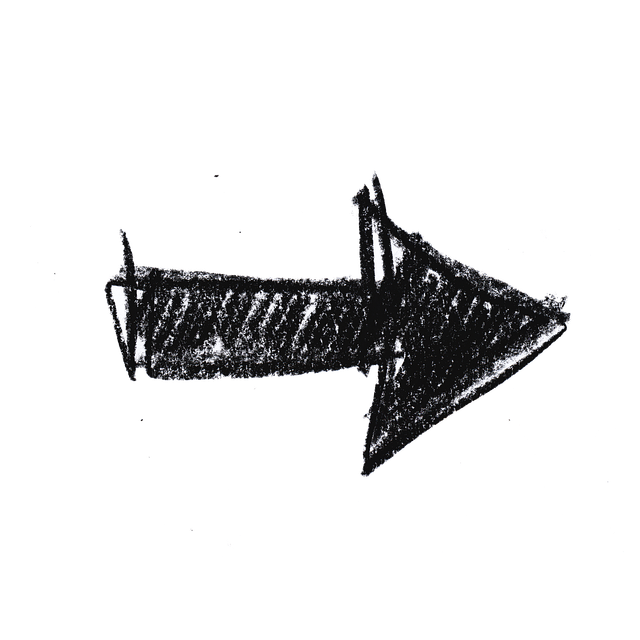
\includegraphics[width=\textwidth]{arrow.png}
      \end{column}
      \begin{column}{0.40\textwidth}
        \begin{itemize}
          \item \structure{$>100 \times$} speedup
          \item provable tractability
        \end{itemize}
      \end{column}
    \end{columns}
  \end{block}
\end{frame}

\begin{frame}{Contributions}
  \begin{columns}[t]
    \begin{column}{0.46\textwidth}
      \centering
      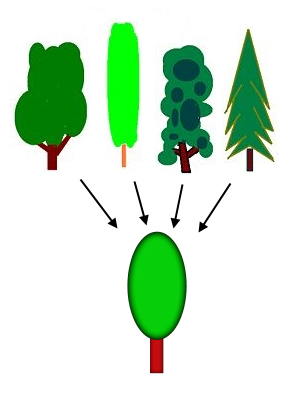
\includegraphics[width=0.5\textwidth]{trees.png}
      \begin{block}{Generalising Representations}
        \begin{itemize}
          \item Beyond weights on literals
          \item Circuits for recursion
        \end{itemize}
      \end{block}
    \end{column}
    \begin{column}{0.54\textwidth}
      \centering
      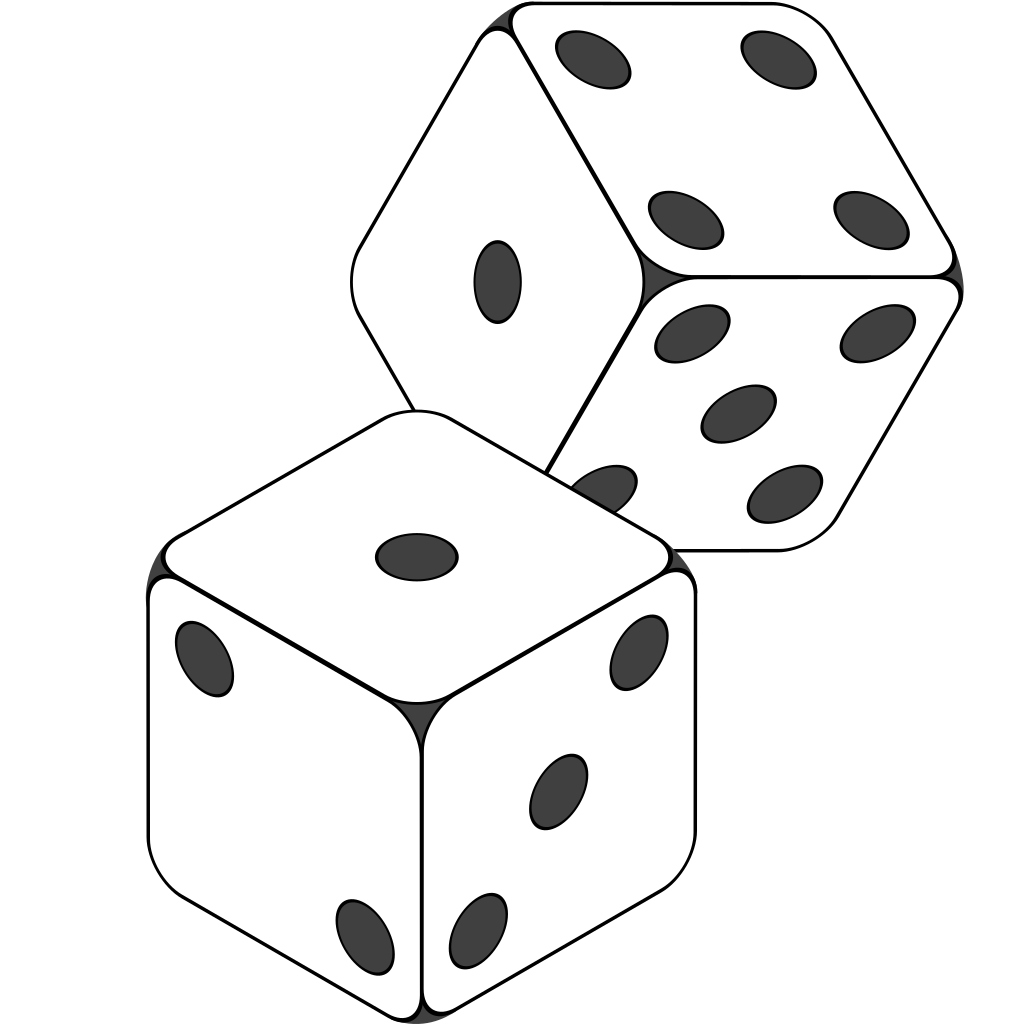
\includegraphics[width=0.5\textwidth]{dice}
      \begin{block}{Random-Instance Experiments}
        \begin{itemize}
          \item Application-specific parameters%
          \begin{itemize}
            \item \textsc{ProbLog} predicates, arities
          \end{itemize}
          \item Parameters of hardness
          \begin{itemize}
            \item density, primal treewidth
          \end{itemize}
        \end{itemize}
      \end{block}
    \end{column}
  \end{columns}
\end{frame}

\begin{frame}
  \vfill
  \centering
  \begin{beamercolorbox}[sep=8pt,center,shadow=true,rounded=true]{title}
    \usebeamerfont{title}Generalising Representations\par%
  \end{beamercolorbox}
  \vfill
\end{frame}

\begin{frame}{WMC and Measures on Boolean Algebras}
  \begin{definition}
    A \alert{measure} is a function
    \structure{$\mu\colon \mathcal{P}(\mathcal{P}(X)) \to \mathbb{R}_{\ge 0}$}
    such that:
    \begin{itemize}
      \item \structure{$\mu(\bot) = 0$};
      \item \structure{$\mu(x \lor y) = \mu(x) + \mu(y)$} whenever
            \structure{$x \land y = \bot$}.
    \end{itemize}
  \end{definition}
  \begin{block}{Observation}
    WMC corresponds to the process of calculating the value of
    \structure{$\mu(x)$} for some
    \structure{$x \in \mathcal{P}(\mathcal{P}(X))$}.
  \end{block}
  \begin{block}{Observation}
    Classical WMC is only able to evaluate \alert{factorable} measures (c.f., a
    collection of mutually independent random variables).
  \end{block}
  \begin{theorem}[Informal Version]
    It is always possible to add more variables to turn a non-factorable measure
    into a factorable measure.
  \end{theorem}
  However, that is not necessarily a good idea!
\end{frame}

\begin{frame}{Experiments with Bayesian Networks}
    \hspace*{-0.5cm}% Created by tikzDevice version 0.12.3.1 on 2021-06-01 14:27:09
% !TEX encoding = UTF-8 Unicode
\begin{tikzpicture}[x=1pt,y=1pt]
\definecolor{fillColor}{RGB}{255,255,255}
\path[use as bounding box,fill=fillColor,fill opacity=0.00] (0,0) rectangle (343.28,231.26);
\begin{scope}
\path[clip] (  0.00,  0.09) rectangle (343.28,231.18);
\definecolor{drawColor}{RGB}{255,255,255}
\definecolor{fillColor}{RGB}{255,255,255}

\path[draw=drawColor,line width= 0.6pt,line join=round,line cap=round,fill=fillColor] (  0.00,  0.09) rectangle (343.28,231.18);
\end{scope}
\begin{scope}
\path[clip] ( 40.51, 30.77) rectangle (235.42,225.68);
\definecolor{fillColor}{RGB}{255,255,255}

\path[fill=fillColor] ( 40.51, 30.77) rectangle (235.42,225.68);
\definecolor{drawColor}{gray}{0.87}

\path[draw=drawColor,line width= 0.1pt,line join=round] ( 40.51, 39.63) --
	(235.42, 39.63);

\path[draw=drawColor,line width= 0.1pt,line join=round] ( 40.51,106.48) --
	(235.42,106.48);

\path[draw=drawColor,line width= 0.1pt,line join=round] ( 40.51,173.33) --
	(235.42,173.33);

\path[draw=drawColor,line width= 0.1pt,line join=round] ( 49.37, 30.77) --
	( 49.37,225.68);

\path[draw=drawColor,line width= 0.1pt,line join=round] (116.22, 30.77) --
	(116.22,225.68);

\path[draw=drawColor,line width= 0.1pt,line join=round] (183.07, 30.77) --
	(183.07,225.68);

\path[draw=drawColor,line width= 0.3pt,line join=round] ( 40.51, 73.06) --
	(235.42, 73.06);

\path[draw=drawColor,line width= 0.3pt,line join=round] ( 40.51,139.91) --
	(235.42,139.91);

\path[draw=drawColor,line width= 0.3pt,line join=round] ( 40.51,206.76) --
	(235.42,206.76);

\path[draw=drawColor,line width= 0.3pt,line join=round] ( 82.79, 30.77) --
	( 82.79,225.68);

\path[draw=drawColor,line width= 0.3pt,line join=round] (149.64, 30.77) --
	(149.64,225.68);

\path[draw=drawColor,line width= 0.3pt,line join=round] (216.49, 30.77) --
	(216.49,225.68);
\definecolor{drawColor}{RGB}{230,171,2}

\path[draw=drawColor,draw opacity=0.50,line width= 0.4pt,line join=round,line cap=round] (133.18,215.39) -- (136.04,218.25);

\path[draw=drawColor,draw opacity=0.50,line width= 0.4pt,line join=round,line cap=round] (133.18,218.25) -- (136.04,215.39);

\path[draw=drawColor,draw opacity=0.50,line width= 0.4pt,line join=round,line cap=round] (132.59,216.82) -- (136.63,216.82);

\path[draw=drawColor,draw opacity=0.50,line width= 0.4pt,line join=round,line cap=round] (134.61,214.80) -- (134.61,218.84);

\path[draw=drawColor,draw opacity=0.50,line width= 0.4pt,line join=round,line cap=round] (134.21,215.39) -- (137.06,218.25);

\path[draw=drawColor,draw opacity=0.50,line width= 0.4pt,line join=round,line cap=round] (134.21,218.25) -- (137.06,215.39);

\path[draw=drawColor,draw opacity=0.50,line width= 0.4pt,line join=round,line cap=round] (133.62,216.82) -- (137.65,216.82);

\path[draw=drawColor,draw opacity=0.50,line width= 0.4pt,line join=round,line cap=round] (135.64,214.80) -- (135.64,218.84);

\path[draw=drawColor,draw opacity=0.50,line width= 0.4pt,line join=round,line cap=round] (134.25,215.39) -- (137.10,218.25);

\path[draw=drawColor,draw opacity=0.50,line width= 0.4pt,line join=round,line cap=round] (134.25,218.25) -- (137.10,215.39);

\path[draw=drawColor,draw opacity=0.50,line width= 0.4pt,line join=round,line cap=round] (133.66,216.82) -- (137.69,216.82);

\path[draw=drawColor,draw opacity=0.50,line width= 0.4pt,line join=round,line cap=round] (135.68,214.80) -- (135.68,218.84);

\path[draw=drawColor,draw opacity=0.50,line width= 0.4pt,line join=round,line cap=round] (137.53,215.39) -- (140.39,218.25);

\path[draw=drawColor,draw opacity=0.50,line width= 0.4pt,line join=round,line cap=round] (137.53,218.25) -- (140.39,215.39);

\path[draw=drawColor,draw opacity=0.50,line width= 0.4pt,line join=round,line cap=round] (136.94,216.82) -- (140.98,216.82);

\path[draw=drawColor,draw opacity=0.50,line width= 0.4pt,line join=round,line cap=round] (138.96,214.80) -- (138.96,218.84);

\path[draw=drawColor,draw opacity=0.50,line width= 0.4pt,line join=round,line cap=round] (133.55,215.39) -- (136.40,218.25);

\path[draw=drawColor,draw opacity=0.50,line width= 0.4pt,line join=round,line cap=round] (133.55,218.25) -- (136.40,215.39);

\path[draw=drawColor,draw opacity=0.50,line width= 0.4pt,line join=round,line cap=round] (132.96,216.82) -- (136.99,216.82);

\path[draw=drawColor,draw opacity=0.50,line width= 0.4pt,line join=round,line cap=round] (134.97,214.80) -- (134.97,218.84);

\path[draw=drawColor,draw opacity=0.50,line width= 0.4pt,line join=round,line cap=round] (134.29,215.39) -- (137.14,218.25);

\path[draw=drawColor,draw opacity=0.50,line width= 0.4pt,line join=round,line cap=round] (134.29,218.25) -- (137.14,215.39);

\path[draw=drawColor,draw opacity=0.50,line width= 0.4pt,line join=round,line cap=round] (133.70,216.82) -- (137.73,216.82);

\path[draw=drawColor,draw opacity=0.50,line width= 0.4pt,line join=round,line cap=round] (135.71,214.80) -- (135.71,218.84);

\path[draw=drawColor,draw opacity=0.50,line width= 0.4pt,line join=round,line cap=round] (135.13,101.07) -- (137.99,103.92);

\path[draw=drawColor,draw opacity=0.50,line width= 0.4pt,line join=round,line cap=round] (135.13,103.92) -- (137.99,101.07);

\path[draw=drawColor,draw opacity=0.50,line width= 0.4pt,line join=round,line cap=round] (134.54,102.50) -- (138.58,102.50);

\path[draw=drawColor,draw opacity=0.50,line width= 0.4pt,line join=round,line cap=round] (136.56,100.48) -- (136.56,104.52);

\path[draw=drawColor,draw opacity=0.50,line width= 0.4pt,line join=round,line cap=round] (133.94,101.26) -- (136.79,104.11);

\path[draw=drawColor,draw opacity=0.50,line width= 0.4pt,line join=round,line cap=round] (133.94,104.11) -- (136.79,101.26);

\path[draw=drawColor,draw opacity=0.50,line width= 0.4pt,line join=round,line cap=round] (133.35,102.69) -- (137.39,102.69);

\path[draw=drawColor,draw opacity=0.50,line width= 0.4pt,line join=round,line cap=round] (135.37,100.67) -- (135.37,104.70);

\path[draw=drawColor,draw opacity=0.50,line width= 0.4pt,line join=round,line cap=round] (135.93,101.45) -- (138.79,104.30);

\path[draw=drawColor,draw opacity=0.50,line width= 0.4pt,line join=round,line cap=round] (135.93,104.30) -- (138.79,101.45);

\path[draw=drawColor,draw opacity=0.50,line width= 0.4pt,line join=round,line cap=round] (135.34,102.87) -- (139.38,102.87);

\path[draw=drawColor,draw opacity=0.50,line width= 0.4pt,line join=round,line cap=round] (137.36,100.86) -- (137.36,104.89);

\path[draw=drawColor,draw opacity=0.50,line width= 0.4pt,line join=round,line cap=round] (130.84, 97.15) -- (133.69,100.00);

\path[draw=drawColor,draw opacity=0.50,line width= 0.4pt,line join=round,line cap=round] (130.84,100.00) -- (133.69, 97.15);

\path[draw=drawColor,draw opacity=0.50,line width= 0.4pt,line join=round,line cap=round] (130.25, 98.57) -- (134.28, 98.57);

\path[draw=drawColor,draw opacity=0.50,line width= 0.4pt,line join=round,line cap=round] (132.26, 96.56) -- (132.26,100.59);

\path[draw=drawColor,draw opacity=0.50,line width= 0.4pt,line join=round,line cap=round] (133.59, 98.35) -- (136.44,101.20);

\path[draw=drawColor,draw opacity=0.50,line width= 0.4pt,line join=round,line cap=round] (133.59,101.20) -- (136.44, 98.35);

\path[draw=drawColor,draw opacity=0.50,line width= 0.4pt,line join=round,line cap=round] (133.00, 99.77) -- (137.03, 99.77);

\path[draw=drawColor,draw opacity=0.50,line width= 0.4pt,line join=round,line cap=round] (135.01, 97.76) -- (135.01,101.79);

\path[draw=drawColor,draw opacity=0.50,line width= 0.4pt,line join=round,line cap=round] (133.67,215.39) -- (136.52,218.25);

\path[draw=drawColor,draw opacity=0.50,line width= 0.4pt,line join=round,line cap=round] (133.67,218.25) -- (136.52,215.39);

\path[draw=drawColor,draw opacity=0.50,line width= 0.4pt,line join=round,line cap=round] (133.08,216.82) -- (137.11,216.82);

\path[draw=drawColor,draw opacity=0.50,line width= 0.4pt,line join=round,line cap=round] (135.09,214.80) -- (135.09,218.84);

\path[draw=drawColor,draw opacity=0.50,line width= 0.4pt,line join=round,line cap=round] (137.20,215.39) -- (140.05,218.25);

\path[draw=drawColor,draw opacity=0.50,line width= 0.4pt,line join=round,line cap=round] (137.20,218.25) -- (140.05,215.39);

\path[draw=drawColor,draw opacity=0.50,line width= 0.4pt,line join=round,line cap=round] (136.61,216.82) -- (140.64,216.82);

\path[draw=drawColor,draw opacity=0.50,line width= 0.4pt,line join=round,line cap=round] (138.62,214.80) -- (138.62,218.84);

\path[draw=drawColor,draw opacity=0.50,line width= 0.4pt,line join=round,line cap=round] (133.51,215.39) -- (136.36,218.25);

\path[draw=drawColor,draw opacity=0.50,line width= 0.4pt,line join=round,line cap=round] (133.51,218.25) -- (136.36,215.39);

\path[draw=drawColor,draw opacity=0.50,line width= 0.4pt,line join=round,line cap=round] (132.92,216.82) -- (136.95,216.82);

\path[draw=drawColor,draw opacity=0.50,line width= 0.4pt,line join=round,line cap=round] (134.93,214.80) -- (134.93,218.84);

\path[draw=drawColor,draw opacity=0.50,line width= 0.4pt,line join=round,line cap=round] (134.36,215.39) -- (137.22,218.25);

\path[draw=drawColor,draw opacity=0.50,line width= 0.4pt,line join=round,line cap=round] (134.36,218.25) -- (137.22,215.39);

\path[draw=drawColor,draw opacity=0.50,line width= 0.4pt,line join=round,line cap=round] (133.77,216.82) -- (137.81,216.82);

\path[draw=drawColor,draw opacity=0.50,line width= 0.4pt,line join=round,line cap=round] (135.79,214.80) -- (135.79,218.84);

\path[draw=drawColor,draw opacity=0.50,line width= 0.4pt,line join=round,line cap=round] (133.27,215.39) -- (136.12,218.25);

\path[draw=drawColor,draw opacity=0.50,line width= 0.4pt,line join=round,line cap=round] (133.27,218.25) -- (136.12,215.39);

\path[draw=drawColor,draw opacity=0.50,line width= 0.4pt,line join=round,line cap=round] (132.68,216.82) -- (136.71,216.82);

\path[draw=drawColor,draw opacity=0.50,line width= 0.4pt,line join=round,line cap=round] (134.69,214.80) -- (134.69,218.84);

\path[draw=drawColor,draw opacity=0.50,line width= 0.4pt,line join=round,line cap=round] (137.10,112.67) -- (139.96,115.53);

\path[draw=drawColor,draw opacity=0.50,line width= 0.4pt,line join=round,line cap=round] (137.10,115.53) -- (139.96,112.67);

\path[draw=drawColor,draw opacity=0.50,line width= 0.4pt,line join=round,line cap=round] (136.51,114.10) -- (140.55,114.10);

\path[draw=drawColor,draw opacity=0.50,line width= 0.4pt,line join=round,line cap=round] (138.53,112.08) -- (138.53,116.12);

\path[draw=drawColor,draw opacity=0.50,line width= 0.4pt,line join=round,line cap=round] (135.49,106.70) -- (138.34,109.55);

\path[draw=drawColor,draw opacity=0.50,line width= 0.4pt,line join=round,line cap=round] (135.49,109.55) -- (138.34,106.70);

\path[draw=drawColor,draw opacity=0.50,line width= 0.4pt,line join=round,line cap=round] (134.90,108.13) -- (138.93,108.13);

\path[draw=drawColor,draw opacity=0.50,line width= 0.4pt,line join=round,line cap=round] (136.91,106.11) -- (136.91,110.14);

\path[draw=drawColor,draw opacity=0.50,line width= 0.4pt,line join=round,line cap=round] (135.90,106.57) -- (138.75,109.42);

\path[draw=drawColor,draw opacity=0.50,line width= 0.4pt,line join=round,line cap=round] (135.90,109.42) -- (138.75,106.57);

\path[draw=drawColor,draw opacity=0.50,line width= 0.4pt,line join=round,line cap=round] (135.31,108.00) -- (139.34,108.00);

\path[draw=drawColor,draw opacity=0.50,line width= 0.4pt,line join=round,line cap=round] (137.33,105.98) -- (137.33,110.01);

\path[draw=drawColor,draw opacity=0.50,line width= 0.4pt,line join=round,line cap=round] (135.10,105.90) -- (137.95,108.75);

\path[draw=drawColor,draw opacity=0.50,line width= 0.4pt,line join=round,line cap=round] (135.10,108.75) -- (137.95,105.90);

\path[draw=drawColor,draw opacity=0.50,line width= 0.4pt,line join=round,line cap=round] (134.51,107.33) -- (138.54,107.33);

\path[draw=drawColor,draw opacity=0.50,line width= 0.4pt,line join=round,line cap=round] (136.52,105.31) -- (136.52,109.34);

\path[draw=drawColor,draw opacity=0.50,line width= 0.4pt,line join=round,line cap=round] (137.50,107.33) -- (140.36,110.19);

\path[draw=drawColor,draw opacity=0.50,line width= 0.4pt,line join=round,line cap=round] (137.50,110.19) -- (140.36,107.33);

\path[draw=drawColor,draw opacity=0.50,line width= 0.4pt,line join=round,line cap=round] (136.91,108.76) -- (140.95,108.76);

\path[draw=drawColor,draw opacity=0.50,line width= 0.4pt,line join=round,line cap=round] (138.93,106.74) -- (138.93,110.78);

\path[draw=drawColor,draw opacity=0.50,line width= 0.4pt,line join=round,line cap=round] (136.69,106.57) -- (139.54,109.42);

\path[draw=drawColor,draw opacity=0.50,line width= 0.4pt,line join=round,line cap=round] (136.69,109.42) -- (139.54,106.57);

\path[draw=drawColor,draw opacity=0.50,line width= 0.4pt,line join=round,line cap=round] (136.10,108.00) -- (140.14,108.00);

\path[draw=drawColor,draw opacity=0.50,line width= 0.4pt,line join=round,line cap=round] (138.12,105.98) -- (138.12,110.01);

\path[draw=drawColor,draw opacity=0.50,line width= 0.4pt,line join=round,line cap=round] (134.66,100.08) -- (137.51,102.94);

\path[draw=drawColor,draw opacity=0.50,line width= 0.4pt,line join=round,line cap=round] (134.66,102.94) -- (137.51,100.08);

\path[draw=drawColor,draw opacity=0.50,line width= 0.4pt,line join=round,line cap=round] (134.07,101.51) -- (138.10,101.51);

\path[draw=drawColor,draw opacity=0.50,line width= 0.4pt,line join=round,line cap=round] (136.09, 99.49) -- (136.09,103.53);

\path[draw=drawColor,draw opacity=0.50,line width= 0.4pt,line join=round,line cap=round] (134.92,101.07) -- (137.77,103.92);

\path[draw=drawColor,draw opacity=0.50,line width= 0.4pt,line join=round,line cap=round] (134.92,103.92) -- (137.77,101.07);

\path[draw=drawColor,draw opacity=0.50,line width= 0.4pt,line join=round,line cap=round] (134.33,102.50) -- (138.36,102.50);

\path[draw=drawColor,draw opacity=0.50,line width= 0.4pt,line join=round,line cap=round] (136.34,100.48) -- (136.34,104.52);

\path[draw=drawColor,draw opacity=0.50,line width= 0.4pt,line join=round,line cap=round] (132.94,101.07) -- (135.79,103.92);

\path[draw=drawColor,draw opacity=0.50,line width= 0.4pt,line join=round,line cap=round] (132.94,103.92) -- (135.79,101.07);

\path[draw=drawColor,draw opacity=0.50,line width= 0.4pt,line join=round,line cap=round] (132.35,102.50) -- (136.38,102.50);

\path[draw=drawColor,draw opacity=0.50,line width= 0.4pt,line join=round,line cap=round] (134.36,100.48) -- (134.36,104.52);

\path[draw=drawColor,draw opacity=0.50,line width= 0.4pt,line join=round,line cap=round] (136.23,104.46) -- (139.09,107.32);

\path[draw=drawColor,draw opacity=0.50,line width= 0.4pt,line join=round,line cap=round] (136.23,107.32) -- (139.09,104.46);

\path[draw=drawColor,draw opacity=0.50,line width= 0.4pt,line join=round,line cap=round] (135.64,105.89) -- (139.68,105.89);

\path[draw=drawColor,draw opacity=0.50,line width= 0.4pt,line join=round,line cap=round] (137.66,103.87) -- (137.66,107.91);

\path[draw=drawColor,draw opacity=0.50,line width= 0.4pt,line join=round,line cap=round] (133.31,102.17) -- (136.16,105.03);

\path[draw=drawColor,draw opacity=0.50,line width= 0.4pt,line join=round,line cap=round] (133.31,105.03) -- (136.16,102.17);

\path[draw=drawColor,draw opacity=0.50,line width= 0.4pt,line join=round,line cap=round] (132.72,103.60) -- (136.75,103.60);

\path[draw=drawColor,draw opacity=0.50,line width= 0.4pt,line join=round,line cap=round] (134.73,101.58) -- (134.73,105.62);

\path[draw=drawColor,draw opacity=0.50,line width= 0.4pt,line join=round,line cap=round] (134.44,106.17) -- (137.29,109.03);

\path[draw=drawColor,draw opacity=0.50,line width= 0.4pt,line join=round,line cap=round] (134.44,109.03) -- (137.29,106.17);

\path[draw=drawColor,draw opacity=0.50,line width= 0.4pt,line join=round,line cap=round] (133.85,107.60) -- (137.88,107.60);

\path[draw=drawColor,draw opacity=0.50,line width= 0.4pt,line join=round,line cap=round] (135.86,105.58) -- (135.86,109.62);

\path[draw=drawColor,draw opacity=0.50,line width= 0.4pt,line join=round,line cap=round] (136.07,106.44) -- (138.92,109.29);

\path[draw=drawColor,draw opacity=0.50,line width= 0.4pt,line join=round,line cap=round] (136.07,109.29) -- (138.92,106.44);

\path[draw=drawColor,draw opacity=0.50,line width= 0.4pt,line join=round,line cap=round] (135.48,107.86) -- (139.51,107.86);

\path[draw=drawColor,draw opacity=0.50,line width= 0.4pt,line join=round,line cap=round] (137.49,105.85) -- (137.49,109.88);

\path[draw=drawColor,draw opacity=0.50,line width= 0.4pt,line join=round,line cap=round] (137.29,107.94) -- (140.14,110.79);

\path[draw=drawColor,draw opacity=0.50,line width= 0.4pt,line join=round,line cap=round] (137.29,110.79) -- (140.14,107.94);

\path[draw=drawColor,draw opacity=0.50,line width= 0.4pt,line join=round,line cap=round] (136.70,109.37) -- (140.73,109.37);

\path[draw=drawColor,draw opacity=0.50,line width= 0.4pt,line join=round,line cap=round] (138.72,107.35) -- (138.72,111.39);

\path[draw=drawColor,draw opacity=0.50,line width= 0.4pt,line join=round,line cap=round] (137.83,107.58) -- (140.69,110.43);

\path[draw=drawColor,draw opacity=0.50,line width= 0.4pt,line join=round,line cap=round] (137.83,110.43) -- (140.69,107.58);

\path[draw=drawColor,draw opacity=0.50,line width= 0.4pt,line join=round,line cap=round] (137.24,109.01) -- (141.28,109.01);

\path[draw=drawColor,draw opacity=0.50,line width= 0.4pt,line join=round,line cap=round] (139.26,106.99) -- (139.26,111.02);

\path[draw=drawColor,draw opacity=0.50,line width= 0.4pt,line join=round,line cap=round] (136.85,107.33) -- (139.70,110.19);

\path[draw=drawColor,draw opacity=0.50,line width= 0.4pt,line join=round,line cap=round] (136.85,110.19) -- (139.70,107.33);

\path[draw=drawColor,draw opacity=0.50,line width= 0.4pt,line join=round,line cap=round] (136.26,108.76) -- (140.29,108.76);

\path[draw=drawColor,draw opacity=0.50,line width= 0.4pt,line join=round,line cap=round] (138.28,106.74) -- (138.28,110.78);

\path[draw=drawColor,draw opacity=0.50,line width= 0.4pt,line join=round,line cap=round] (136.69,112.24) -- (139.54,115.09);

\path[draw=drawColor,draw opacity=0.50,line width= 0.4pt,line join=round,line cap=round] (136.69,115.09) -- (139.54,112.24);

\path[draw=drawColor,draw opacity=0.50,line width= 0.4pt,line join=round,line cap=round] (136.10,113.66) -- (140.14,113.66);

\path[draw=drawColor,draw opacity=0.50,line width= 0.4pt,line join=round,line cap=round] (138.12,111.64) -- (138.12,115.68);

\path[draw=drawColor,draw opacity=0.50,line width= 0.4pt,line join=round,line cap=round] (137.17,111.04) -- (140.02,113.89);

\path[draw=drawColor,draw opacity=0.50,line width= 0.4pt,line join=round,line cap=round] (137.17,113.89) -- (140.02,111.04);

\path[draw=drawColor,draw opacity=0.50,line width= 0.4pt,line join=round,line cap=round] (136.57,112.46) -- (140.61,112.46);

\path[draw=drawColor,draw opacity=0.50,line width= 0.4pt,line join=round,line cap=round] (138.59,110.45) -- (138.59,114.48);

\path[draw=drawColor,draw opacity=0.50,line width= 0.4pt,line join=round,line cap=round] (135.97,114.75) -- (138.82,117.60);

\path[draw=drawColor,draw opacity=0.50,line width= 0.4pt,line join=round,line cap=round] (135.97,117.60) -- (138.82,114.75);

\path[draw=drawColor,draw opacity=0.50,line width= 0.4pt,line join=round,line cap=round] (135.38,116.18) -- (139.41,116.18);

\path[draw=drawColor,draw opacity=0.50,line width= 0.4pt,line join=round,line cap=round] (137.39,114.16) -- (137.39,118.19);

\path[draw=drawColor,draw opacity=0.50,line width= 0.4pt,line join=round,line cap=round] (136.50,112.67) -- (139.35,115.53);

\path[draw=drawColor,draw opacity=0.50,line width= 0.4pt,line join=round,line cap=round] (136.50,115.53) -- (139.35,112.67);

\path[draw=drawColor,draw opacity=0.50,line width= 0.4pt,line join=round,line cap=round] (135.91,114.10) -- (139.94,114.10);

\path[draw=drawColor,draw opacity=0.50,line width= 0.4pt,line join=round,line cap=round] (137.92,112.08) -- (137.92,116.12);

\path[draw=drawColor,draw opacity=0.50,line width= 0.4pt,line join=round,line cap=round] (137.95,116.50) -- (140.80,119.35);

\path[draw=drawColor,draw opacity=0.50,line width= 0.4pt,line join=round,line cap=round] (137.95,119.35) -- (140.80,116.50);

\path[draw=drawColor,draw opacity=0.50,line width= 0.4pt,line join=round,line cap=round] (137.36,117.93) -- (141.40,117.93);

\path[draw=drawColor,draw opacity=0.50,line width= 0.4pt,line join=round,line cap=round] (139.38,115.91) -- (139.38,119.94);

\path[draw=drawColor,draw opacity=0.50,line width= 0.4pt,line join=round,line cap=round] (138.19,111.42) -- (141.04,114.27);

\path[draw=drawColor,draw opacity=0.50,line width= 0.4pt,line join=round,line cap=round] (138.19,114.27) -- (141.04,111.42);

\path[draw=drawColor,draw opacity=0.50,line width= 0.4pt,line join=round,line cap=round] (137.59,112.84) -- (141.63,112.84);

\path[draw=drawColor,draw opacity=0.50,line width= 0.4pt,line join=round,line cap=round] (139.61,110.83) -- (139.61,114.86);

\path[draw=drawColor,draw opacity=0.50,line width= 0.4pt,line join=round,line cap=round] (138.10,111.60) -- (140.95,114.46);

\path[draw=drawColor,draw opacity=0.50,line width= 0.4pt,line join=round,line cap=round] (138.10,114.46) -- (140.95,111.60);

\path[draw=drawColor,draw opacity=0.50,line width= 0.4pt,line join=round,line cap=round] (137.51,113.03) -- (141.54,113.03);

\path[draw=drawColor,draw opacity=0.50,line width= 0.4pt,line join=round,line cap=round] (139.52,111.01) -- (139.52,115.05);

\path[draw=drawColor,draw opacity=0.50,line width= 0.4pt,line join=round,line cap=round] (135.35,105.05) -- (138.20,107.91);

\path[draw=drawColor,draw opacity=0.50,line width= 0.4pt,line join=round,line cap=round] (135.35,107.91) -- (138.20,105.05);

\path[draw=drawColor,draw opacity=0.50,line width= 0.4pt,line join=round,line cap=round] (134.76,106.48) -- (138.79,106.48);

\path[draw=drawColor,draw opacity=0.50,line width= 0.4pt,line join=round,line cap=round] (136.77,104.46) -- (136.77,108.50);

\path[draw=drawColor,draw opacity=0.50,line width= 0.4pt,line join=round,line cap=round] (137.17,107.70) -- (140.02,110.55);

\path[draw=drawColor,draw opacity=0.50,line width= 0.4pt,line join=round,line cap=round] (137.17,110.55) -- (140.02,107.70);

\path[draw=drawColor,draw opacity=0.50,line width= 0.4pt,line join=round,line cap=round] (136.57,109.13) -- (140.61,109.13);

\path[draw=drawColor,draw opacity=0.50,line width= 0.4pt,line join=round,line cap=round] (138.59,107.11) -- (138.59,111.15);

\path[draw=drawColor,draw opacity=0.50,line width= 0.4pt,line join=round,line cap=round] (137.35,112.59) -- (140.20,115.44);

\path[draw=drawColor,draw opacity=0.50,line width= 0.4pt,line join=round,line cap=round] (137.35,115.44) -- (140.20,112.59);

\path[draw=drawColor,draw opacity=0.50,line width= 0.4pt,line join=round,line cap=round] (136.76,114.01) -- (140.79,114.01);

\path[draw=drawColor,draw opacity=0.50,line width= 0.4pt,line join=round,line cap=round] (138.78,111.99) -- (138.78,116.03);

\path[draw=drawColor,draw opacity=0.50,line width= 0.4pt,line join=round,line cap=round] (136.63,105.48) -- (139.48,108.34);

\path[draw=drawColor,draw opacity=0.50,line width= 0.4pt,line join=round,line cap=round] (136.63,108.34) -- (139.48,105.48);

\path[draw=drawColor,draw opacity=0.50,line width= 0.4pt,line join=round,line cap=round] (136.04,106.91) -- (140.07,106.91);

\path[draw=drawColor,draw opacity=0.50,line width= 0.4pt,line join=round,line cap=round] (138.05,104.89) -- (138.05,108.93);

\path[draw=drawColor,draw opacity=0.50,line width= 0.4pt,line join=round,line cap=round] (138.81,121.10) -- (141.66,123.95);

\path[draw=drawColor,draw opacity=0.50,line width= 0.4pt,line join=round,line cap=round] (138.81,123.95) -- (141.66,121.10);

\path[draw=drawColor,draw opacity=0.50,line width= 0.4pt,line join=round,line cap=round] (138.22,122.53) -- (142.25,122.53);

\path[draw=drawColor,draw opacity=0.50,line width= 0.4pt,line join=round,line cap=round] (140.24,120.51) -- (140.24,124.54);

\path[draw=drawColor,draw opacity=0.50,line width= 0.4pt,line join=round,line cap=round] (136.37,116.43) -- (139.22,119.29);

\path[draw=drawColor,draw opacity=0.50,line width= 0.4pt,line join=round,line cap=round] (136.37,119.29) -- (139.22,116.43);

\path[draw=drawColor,draw opacity=0.50,line width= 0.4pt,line join=round,line cap=round] (135.78,117.86) -- (139.81,117.86);

\path[draw=drawColor,draw opacity=0.50,line width= 0.4pt,line join=round,line cap=round] (137.79,115.84) -- (137.79,119.88);

\path[draw=drawColor,draw opacity=0.50,line width= 0.4pt,line join=round,line cap=round] (135.35,109.84) -- (138.20,112.69);

\path[draw=drawColor,draw opacity=0.50,line width= 0.4pt,line join=round,line cap=round] (135.35,112.69) -- (138.20,109.84);

\path[draw=drawColor,draw opacity=0.50,line width= 0.4pt,line join=round,line cap=round] (134.76,111.26) -- (138.79,111.26);

\path[draw=drawColor,draw opacity=0.50,line width= 0.4pt,line join=round,line cap=round] (136.77,109.24) -- (136.77,113.28);

\path[draw=drawColor,draw opacity=0.50,line width= 0.4pt,line join=round,line cap=round] (136.69,109.19) -- (139.54,112.05);

\path[draw=drawColor,draw opacity=0.50,line width= 0.4pt,line join=round,line cap=round] (136.69,112.05) -- (139.54,109.19);

\path[draw=drawColor,draw opacity=0.50,line width= 0.4pt,line join=round,line cap=round] (136.10,110.62) -- (140.14,110.62);

\path[draw=drawColor,draw opacity=0.50,line width= 0.4pt,line join=round,line cap=round] (138.12,108.60) -- (138.12,112.64);

\path[draw=drawColor,draw opacity=0.50,line width= 0.4pt,line join=round,line cap=round] (135.24,111.23) -- (138.09,114.08);

\path[draw=drawColor,draw opacity=0.50,line width= 0.4pt,line join=round,line cap=round] (135.24,114.08) -- (138.09,111.23);

\path[draw=drawColor,draw opacity=0.50,line width= 0.4pt,line join=round,line cap=round] (134.65,112.65) -- (138.68,112.65);

\path[draw=drawColor,draw opacity=0.50,line width= 0.4pt,line join=round,line cap=round] (136.67,110.64) -- (136.67,114.67);

\path[draw=drawColor,draw opacity=0.50,line width= 0.4pt,line join=round,line cap=round] (150.80,215.39) -- (153.66,218.25);

\path[draw=drawColor,draw opacity=0.50,line width= 0.4pt,line join=round,line cap=round] (150.80,218.25) -- (153.66,215.39);

\path[draw=drawColor,draw opacity=0.50,line width= 0.4pt,line join=round,line cap=round] (150.21,216.82) -- (154.25,216.82);

\path[draw=drawColor,draw opacity=0.50,line width= 0.4pt,line join=round,line cap=round] (152.23,214.80) -- (152.23,218.84);

\path[draw=drawColor,draw opacity=0.50,line width= 0.4pt,line join=round,line cap=round] (145.64,215.39) -- (148.49,218.25);

\path[draw=drawColor,draw opacity=0.50,line width= 0.4pt,line join=round,line cap=round] (145.64,218.25) -- (148.49,215.39);

\path[draw=drawColor,draw opacity=0.50,line width= 0.4pt,line join=round,line cap=round] (145.04,216.82) -- (149.08,216.82);

\path[draw=drawColor,draw opacity=0.50,line width= 0.4pt,line join=round,line cap=round] (147.06,214.80) -- (147.06,218.84);

\path[draw=drawColor,draw opacity=0.50,line width= 0.4pt,line join=round,line cap=round] (147.10,215.39) -- (149.96,218.25);

\path[draw=drawColor,draw opacity=0.50,line width= 0.4pt,line join=round,line cap=round] (147.10,218.25) -- (149.96,215.39);

\path[draw=drawColor,draw opacity=0.50,line width= 0.4pt,line join=round,line cap=round] (146.51,216.82) -- (150.55,216.82);

\path[draw=drawColor,draw opacity=0.50,line width= 0.4pt,line join=round,line cap=round] (148.53,214.80) -- (148.53,218.84);

\path[draw=drawColor,draw opacity=0.50,line width= 0.4pt,line join=round,line cap=round] (154.45,215.39) -- (157.30,218.25);

\path[draw=drawColor,draw opacity=0.50,line width= 0.4pt,line join=round,line cap=round] (154.45,218.25) -- (157.30,215.39);

\path[draw=drawColor,draw opacity=0.50,line width= 0.4pt,line join=round,line cap=round] (153.86,216.82) -- (157.89,216.82);

\path[draw=drawColor,draw opacity=0.50,line width= 0.4pt,line join=round,line cap=round] (155.87,214.80) -- (155.87,218.84);

\path[draw=drawColor,draw opacity=0.50,line width= 0.4pt,line join=round,line cap=round] (147.66,215.39) -- (150.51,218.25);

\path[draw=drawColor,draw opacity=0.50,line width= 0.4pt,line join=round,line cap=round] (147.66,218.25) -- (150.51,215.39);

\path[draw=drawColor,draw opacity=0.50,line width= 0.4pt,line join=round,line cap=round] (147.06,216.82) -- (151.10,216.82);

\path[draw=drawColor,draw opacity=0.50,line width= 0.4pt,line join=round,line cap=round] (149.08,214.80) -- (149.08,218.84);

\path[draw=drawColor,draw opacity=0.50,line width= 0.4pt,line join=round,line cap=round] (152.72,215.39) -- (155.58,218.25);

\path[draw=drawColor,draw opacity=0.50,line width= 0.4pt,line join=round,line cap=round] (152.72,218.25) -- (155.58,215.39);

\path[draw=drawColor,draw opacity=0.50,line width= 0.4pt,line join=round,line cap=round] (152.13,216.82) -- (156.17,216.82);

\path[draw=drawColor,draw opacity=0.50,line width= 0.4pt,line join=round,line cap=round] (154.15,214.80) -- (154.15,218.84);

\path[draw=drawColor,draw opacity=0.50,line width= 0.4pt,line join=round,line cap=round] (146.93,187.58) -- (149.78,190.43);

\path[draw=drawColor,draw opacity=0.50,line width= 0.4pt,line join=round,line cap=round] (146.93,190.43) -- (149.78,187.58);

\path[draw=drawColor,draw opacity=0.50,line width= 0.4pt,line join=round,line cap=round] (146.34,189.01) -- (150.37,189.01);

\path[draw=drawColor,draw opacity=0.50,line width= 0.4pt,line join=round,line cap=round] (148.36,186.99) -- (148.36,191.02);

\path[draw=drawColor,draw opacity=0.50,line width= 0.4pt,line join=round,line cap=round] (147.84,155.90) -- (150.69,158.76);

\path[draw=drawColor,draw opacity=0.50,line width= 0.4pt,line join=round,line cap=round] (147.84,158.76) -- (150.69,155.90);

\path[draw=drawColor,draw opacity=0.50,line width= 0.4pt,line join=round,line cap=round] (147.24,157.33) -- (151.28,157.33);

\path[draw=drawColor,draw opacity=0.50,line width= 0.4pt,line join=round,line cap=round] (149.26,155.31) -- (149.26,159.35);

\path[draw=drawColor,draw opacity=0.50,line width= 0.4pt,line join=round,line cap=round] (145.32,152.68) -- (148.17,155.53);

\path[draw=drawColor,draw opacity=0.50,line width= 0.4pt,line join=round,line cap=round] (145.32,155.53) -- (148.17,152.68);

\path[draw=drawColor,draw opacity=0.50,line width= 0.4pt,line join=round,line cap=round] (144.73,154.11) -- (148.76,154.11);

\path[draw=drawColor,draw opacity=0.50,line width= 0.4pt,line join=round,line cap=round] (146.75,152.09) -- (146.75,156.13);

\path[draw=drawColor,draw opacity=0.50,line width= 0.4pt,line join=round,line cap=round] (147.91,156.31) -- (150.76,159.16);

\path[draw=drawColor,draw opacity=0.50,line width= 0.4pt,line join=round,line cap=round] (147.91,159.16) -- (150.76,156.31);

\path[draw=drawColor,draw opacity=0.50,line width= 0.4pt,line join=round,line cap=round] (147.32,157.74) -- (151.35,157.74);

\path[draw=drawColor,draw opacity=0.50,line width= 0.4pt,line join=round,line cap=round] (149.34,155.72) -- (149.34,159.75);

\path[draw=drawColor,draw opacity=0.50,line width= 0.4pt,line join=round,line cap=round] (146.40,153.70) -- (149.25,156.55);

\path[draw=drawColor,draw opacity=0.50,line width= 0.4pt,line join=round,line cap=round] (146.40,156.55) -- (149.25,153.70);

\path[draw=drawColor,draw opacity=0.50,line width= 0.4pt,line join=round,line cap=round] (145.80,155.12) -- (149.84,155.12);

\path[draw=drawColor,draw opacity=0.50,line width= 0.4pt,line join=round,line cap=round] (147.82,153.11) -- (147.82,157.14);

\path[draw=drawColor,draw opacity=0.50,line width= 0.4pt,line join=round,line cap=round] (151.31,215.39) -- (154.16,218.25);

\path[draw=drawColor,draw opacity=0.50,line width= 0.4pt,line join=round,line cap=round] (151.31,218.25) -- (154.16,215.39);

\path[draw=drawColor,draw opacity=0.50,line width= 0.4pt,line join=round,line cap=round] (150.71,216.82) -- (154.75,216.82);

\path[draw=drawColor,draw opacity=0.50,line width= 0.4pt,line join=round,line cap=round] (152.73,214.80) -- (152.73,218.84);

\path[draw=drawColor,draw opacity=0.50,line width= 0.4pt,line join=round,line cap=round] (151.07,215.39) -- (153.92,218.25);

\path[draw=drawColor,draw opacity=0.50,line width= 0.4pt,line join=round,line cap=round] (151.07,218.25) -- (153.92,215.39);

\path[draw=drawColor,draw opacity=0.50,line width= 0.4pt,line join=round,line cap=round] (150.48,216.82) -- (154.51,216.82);

\path[draw=drawColor,draw opacity=0.50,line width= 0.4pt,line join=round,line cap=round] (152.50,214.80) -- (152.50,218.84);

\path[draw=drawColor,draw opacity=0.50,line width= 0.4pt,line join=round,line cap=round] (151.33,215.39) -- (154.18,218.25);

\path[draw=drawColor,draw opacity=0.50,line width= 0.4pt,line join=round,line cap=round] (151.33,218.25) -- (154.18,215.39);

\path[draw=drawColor,draw opacity=0.50,line width= 0.4pt,line join=round,line cap=round] (150.74,216.82) -- (154.77,216.82);

\path[draw=drawColor,draw opacity=0.50,line width= 0.4pt,line join=round,line cap=round] (152.76,214.80) -- (152.76,218.84);

\path[draw=drawColor,draw opacity=0.50,line width= 0.4pt,line join=round,line cap=round] (151.18,215.39) -- (154.03,218.25);

\path[draw=drawColor,draw opacity=0.50,line width= 0.4pt,line join=round,line cap=round] (151.18,218.25) -- (154.03,215.39);

\path[draw=drawColor,draw opacity=0.50,line width= 0.4pt,line join=round,line cap=round] (150.58,216.82) -- (154.62,216.82);

\path[draw=drawColor,draw opacity=0.50,line width= 0.4pt,line join=round,line cap=round] (152.60,214.80) -- (152.60,218.84);

\path[draw=drawColor,draw opacity=0.50,line width= 0.4pt,line join=round,line cap=round] (151.62,215.39) -- (154.47,218.25);

\path[draw=drawColor,draw opacity=0.50,line width= 0.4pt,line join=round,line cap=round] (151.62,218.25) -- (154.47,215.39);

\path[draw=drawColor,draw opacity=0.50,line width= 0.4pt,line join=round,line cap=round] (151.03,216.82) -- (155.06,216.82);

\path[draw=drawColor,draw opacity=0.50,line width= 0.4pt,line join=round,line cap=round] (153.05,214.80) -- (153.05,218.84);

\path[draw=drawColor,draw opacity=0.50,line width= 0.4pt,line join=round,line cap=round] (151.58,215.39) -- (154.44,218.25);

\path[draw=drawColor,draw opacity=0.50,line width= 0.4pt,line join=round,line cap=round] (151.58,218.25) -- (154.44,215.39);

\path[draw=drawColor,draw opacity=0.50,line width= 0.4pt,line join=round,line cap=round] (150.99,216.82) -- (155.03,216.82);

\path[draw=drawColor,draw opacity=0.50,line width= 0.4pt,line join=round,line cap=round] (153.01,214.80) -- (153.01,218.84);

\path[draw=drawColor,draw opacity=0.50,line width= 0.4pt,line join=round,line cap=round] (147.61,215.39) -- (150.46,218.25);

\path[draw=drawColor,draw opacity=0.50,line width= 0.4pt,line join=round,line cap=round] (147.61,218.25) -- (150.46,215.39);

\path[draw=drawColor,draw opacity=0.50,line width= 0.4pt,line join=round,line cap=round] (147.02,216.82) -- (151.05,216.82);

\path[draw=drawColor,draw opacity=0.50,line width= 0.4pt,line join=round,line cap=round] (149.04,214.80) -- (149.04,218.84);

\path[draw=drawColor,draw opacity=0.50,line width= 0.4pt,line join=round,line cap=round] (148.95,215.39) -- (151.81,218.25);

\path[draw=drawColor,draw opacity=0.50,line width= 0.4pt,line join=round,line cap=round] (148.95,218.25) -- (151.81,215.39);

\path[draw=drawColor,draw opacity=0.50,line width= 0.4pt,line join=round,line cap=round] (148.36,216.82) -- (152.40,216.82);

\path[draw=drawColor,draw opacity=0.50,line width= 0.4pt,line join=round,line cap=round] (150.38,214.80) -- (150.38,218.84);

\path[draw=drawColor,draw opacity=0.50,line width= 0.4pt,line join=round,line cap=round] (153.60,215.39) -- (156.46,218.25);

\path[draw=drawColor,draw opacity=0.50,line width= 0.4pt,line join=round,line cap=round] (153.60,218.25) -- (156.46,215.39);

\path[draw=drawColor,draw opacity=0.50,line width= 0.4pt,line join=round,line cap=round] (153.01,216.82) -- (157.05,216.82);

\path[draw=drawColor,draw opacity=0.50,line width= 0.4pt,line join=round,line cap=round] (155.03,214.80) -- (155.03,218.84);

\path[draw=drawColor,draw opacity=0.50,line width= 0.4pt,line join=round,line cap=round] (151.19,215.39) -- (154.04,218.25);

\path[draw=drawColor,draw opacity=0.50,line width= 0.4pt,line join=round,line cap=round] (151.19,218.25) -- (154.04,215.39);

\path[draw=drawColor,draw opacity=0.50,line width= 0.4pt,line join=round,line cap=round] (150.60,216.82) -- (154.63,216.82);

\path[draw=drawColor,draw opacity=0.50,line width= 0.4pt,line join=round,line cap=round] (152.61,214.80) -- (152.61,218.84);

\path[draw=drawColor,draw opacity=0.50,line width= 0.4pt,line join=round,line cap=round] (151.03,215.39) -- (153.89,218.25);

\path[draw=drawColor,draw opacity=0.50,line width= 0.4pt,line join=round,line cap=round] (151.03,218.25) -- (153.89,215.39);

\path[draw=drawColor,draw opacity=0.50,line width= 0.4pt,line join=round,line cap=round] (150.44,216.82) -- (154.48,216.82);

\path[draw=drawColor,draw opacity=0.50,line width= 0.4pt,line join=round,line cap=round] (152.46,214.80) -- (152.46,218.84);

\path[draw=drawColor,draw opacity=0.50,line width= 0.4pt,line join=round,line cap=round] (146.82,155.61) -- (149.67,158.47);

\path[draw=drawColor,draw opacity=0.50,line width= 0.4pt,line join=round,line cap=round] (146.82,158.47) -- (149.67,155.61);

\path[draw=drawColor,draw opacity=0.50,line width= 0.4pt,line join=round,line cap=round] (146.23,157.04) -- (150.26,157.04);

\path[draw=drawColor,draw opacity=0.50,line width= 0.4pt,line join=round,line cap=round] (148.24,155.02) -- (148.24,159.06);

\path[draw=drawColor,draw opacity=0.50,line width= 0.4pt,line join=round,line cap=round] (148.88,158.55) -- (151.74,161.41);

\path[draw=drawColor,draw opacity=0.50,line width= 0.4pt,line join=round,line cap=round] (148.88,161.41) -- (151.74,158.55);

\path[draw=drawColor,draw opacity=0.50,line width= 0.4pt,line join=round,line cap=round] (148.29,159.98) -- (152.33,159.98);

\path[draw=drawColor,draw opacity=0.50,line width= 0.4pt,line join=round,line cap=round] (150.31,157.96) -- (150.31,162.00);

\path[draw=drawColor,draw opacity=0.50,line width= 0.4pt,line join=round,line cap=round] (147.56,154.94) -- (150.42,157.79);

\path[draw=drawColor,draw opacity=0.50,line width= 0.4pt,line join=round,line cap=round] (147.56,157.79) -- (150.42,154.94);

\path[draw=drawColor,draw opacity=0.50,line width= 0.4pt,line join=round,line cap=round] (146.97,156.37) -- (151.01,156.37);

\path[draw=drawColor,draw opacity=0.50,line width= 0.4pt,line join=round,line cap=round] (148.99,154.35) -- (148.99,158.39);

\path[draw=drawColor,draw opacity=0.50,line width= 0.4pt,line join=round,line cap=round] (146.40,156.62) -- (149.25,159.47);

\path[draw=drawColor,draw opacity=0.50,line width= 0.4pt,line join=round,line cap=round] (146.40,159.47) -- (149.25,156.62);

\path[draw=drawColor,draw opacity=0.50,line width= 0.4pt,line join=round,line cap=round] (145.80,158.04) -- (149.84,158.04);

\path[draw=drawColor,draw opacity=0.50,line width= 0.4pt,line join=round,line cap=round] (147.82,156.02) -- (147.82,160.06);

\path[draw=drawColor,draw opacity=0.50,line width= 0.4pt,line join=round,line cap=round] (146.90,155.64) -- (149.75,158.49);

\path[draw=drawColor,draw opacity=0.50,line width= 0.4pt,line join=round,line cap=round] (146.90,158.49) -- (149.75,155.64);

\path[draw=drawColor,draw opacity=0.50,line width= 0.4pt,line join=round,line cap=round] (146.31,157.07) -- (150.34,157.07);

\path[draw=drawColor,draw opacity=0.50,line width= 0.4pt,line join=round,line cap=round] (148.32,155.05) -- (148.32,159.08);

\path[draw=drawColor,draw opacity=0.50,line width= 0.4pt,line join=round,line cap=round] (151.74,215.39) -- (154.60,218.25);

\path[draw=drawColor,draw opacity=0.50,line width= 0.4pt,line join=round,line cap=round] (151.74,218.25) -- (154.60,215.39);

\path[draw=drawColor,draw opacity=0.50,line width= 0.4pt,line join=round,line cap=round] (151.15,216.82) -- (155.19,216.82);

\path[draw=drawColor,draw opacity=0.50,line width= 0.4pt,line join=round,line cap=round] (153.17,214.80) -- (153.17,218.84);

\path[draw=drawColor,draw opacity=0.50,line width= 0.4pt,line join=round,line cap=round] (152.20,215.39) -- (155.06,218.25);

\path[draw=drawColor,draw opacity=0.50,line width= 0.4pt,line join=round,line cap=round] (152.20,218.25) -- (155.06,215.39);

\path[draw=drawColor,draw opacity=0.50,line width= 0.4pt,line join=round,line cap=round] (151.61,216.82) -- (155.65,216.82);

\path[draw=drawColor,draw opacity=0.50,line width= 0.4pt,line join=round,line cap=round] (153.63,214.80) -- (153.63,218.84);

\path[draw=drawColor,draw opacity=0.50,line width= 0.4pt,line join=round,line cap=round] (152.07,215.39) -- (154.92,218.25);

\path[draw=drawColor,draw opacity=0.50,line width= 0.4pt,line join=round,line cap=round] (152.07,218.25) -- (154.92,215.39);

\path[draw=drawColor,draw opacity=0.50,line width= 0.4pt,line join=round,line cap=round] (151.48,216.82) -- (155.52,216.82);

\path[draw=drawColor,draw opacity=0.50,line width= 0.4pt,line join=round,line cap=round] (153.50,214.80) -- (153.50,218.84);

\path[draw=drawColor,draw opacity=0.50,line width= 0.4pt,line join=round,line cap=round] (150.91,215.39) -- (153.77,218.25);

\path[draw=drawColor,draw opacity=0.50,line width= 0.4pt,line join=round,line cap=round] (150.91,218.25) -- (153.77,215.39);

\path[draw=drawColor,draw opacity=0.50,line width= 0.4pt,line join=round,line cap=round] (150.32,216.82) -- (154.36,216.82);

\path[draw=drawColor,draw opacity=0.50,line width= 0.4pt,line join=round,line cap=round] (152.34,214.80) -- (152.34,218.84);

\path[draw=drawColor,draw opacity=0.50,line width= 0.4pt,line join=round,line cap=round] (151.91,215.39) -- (154.77,218.25);

\path[draw=drawColor,draw opacity=0.50,line width= 0.4pt,line join=round,line cap=round] (151.91,218.25) -- (154.77,215.39);

\path[draw=drawColor,draw opacity=0.50,line width= 0.4pt,line join=round,line cap=round] (151.32,216.82) -- (155.36,216.82);

\path[draw=drawColor,draw opacity=0.50,line width= 0.4pt,line join=round,line cap=round] (153.34,214.80) -- (153.34,218.84);

\path[draw=drawColor,draw opacity=0.50,line width= 0.4pt,line join=round,line cap=round] (152.52,215.39) -- (155.37,218.25);

\path[draw=drawColor,draw opacity=0.50,line width= 0.4pt,line join=round,line cap=round] (152.52,218.25) -- (155.37,215.39);

\path[draw=drawColor,draw opacity=0.50,line width= 0.4pt,line join=round,line cap=round] (151.93,216.82) -- (155.96,216.82);

\path[draw=drawColor,draw opacity=0.50,line width= 0.4pt,line join=round,line cap=round] (153.95,214.80) -- (153.95,218.84);

\path[draw=drawColor,draw opacity=0.50,line width= 0.4pt,line join=round,line cap=round] (155.80,215.39) -- (158.65,218.25);

\path[draw=drawColor,draw opacity=0.50,line width= 0.4pt,line join=round,line cap=round] (155.80,218.25) -- (158.65,215.39);

\path[draw=drawColor,draw opacity=0.50,line width= 0.4pt,line join=round,line cap=round] (155.21,216.82) -- (159.25,216.82);

\path[draw=drawColor,draw opacity=0.50,line width= 0.4pt,line join=round,line cap=round] (157.23,214.80) -- (157.23,218.84);

\path[draw=drawColor,draw opacity=0.50,line width= 0.4pt,line join=round,line cap=round] (155.39,215.39) -- (158.24,218.25);

\path[draw=drawColor,draw opacity=0.50,line width= 0.4pt,line join=round,line cap=round] (155.39,218.25) -- (158.24,215.39);

\path[draw=drawColor,draw opacity=0.50,line width= 0.4pt,line join=round,line cap=round] (154.80,216.82) -- (158.83,216.82);

\path[draw=drawColor,draw opacity=0.50,line width= 0.4pt,line join=round,line cap=round] (156.82,214.80) -- (156.82,218.84);

\path[draw=drawColor,draw opacity=0.50,line width= 0.4pt,line join=round,line cap=round] (152.52,215.39) -- (155.37,218.25);

\path[draw=drawColor,draw opacity=0.50,line width= 0.4pt,line join=round,line cap=round] (152.52,218.25) -- (155.37,215.39);

\path[draw=drawColor,draw opacity=0.50,line width= 0.4pt,line join=round,line cap=round] (151.93,216.82) -- (155.96,216.82);

\path[draw=drawColor,draw opacity=0.50,line width= 0.4pt,line join=round,line cap=round] (153.95,214.80) -- (153.95,218.84);

\path[draw=drawColor,draw opacity=0.50,line width= 0.4pt,line join=round,line cap=round] (153.41,215.39) -- (156.26,218.25);

\path[draw=drawColor,draw opacity=0.50,line width= 0.4pt,line join=round,line cap=round] (153.41,218.25) -- (156.26,215.39);

\path[draw=drawColor,draw opacity=0.50,line width= 0.4pt,line join=round,line cap=round] (152.82,216.82) -- (156.85,216.82);

\path[draw=drawColor,draw opacity=0.50,line width= 0.4pt,line join=round,line cap=round] (154.84,214.80) -- (154.84,218.84);

\path[draw=drawColor,draw opacity=0.50,line width= 0.4pt,line join=round,line cap=round] (155.91,215.39) -- (158.77,218.25);

\path[draw=drawColor,draw opacity=0.50,line width= 0.4pt,line join=round,line cap=round] (155.91,218.25) -- (158.77,215.39);

\path[draw=drawColor,draw opacity=0.50,line width= 0.4pt,line join=round,line cap=round] (155.32,216.82) -- (159.36,216.82);

\path[draw=drawColor,draw opacity=0.50,line width= 0.4pt,line join=round,line cap=round] (157.34,214.80) -- (157.34,218.84);

\path[draw=drawColor,draw opacity=0.50,line width= 0.4pt,line join=round,line cap=round] (152.28,215.39) -- (155.13,218.25);

\path[draw=drawColor,draw opacity=0.50,line width= 0.4pt,line join=round,line cap=round] (152.28,218.25) -- (155.13,215.39);

\path[draw=drawColor,draw opacity=0.50,line width= 0.4pt,line join=round,line cap=round] (151.69,216.82) -- (155.73,216.82);

\path[draw=drawColor,draw opacity=0.50,line width= 0.4pt,line join=round,line cap=round] (153.71,214.80) -- (153.71,218.84);

\path[draw=drawColor,draw opacity=0.50,line width= 0.4pt,line join=round,line cap=round] (149.76,160.28) -- (152.61,163.14);

\path[draw=drawColor,draw opacity=0.50,line width= 0.4pt,line join=round,line cap=round] (149.76,163.14) -- (152.61,160.28);

\path[draw=drawColor,draw opacity=0.50,line width= 0.4pt,line join=round,line cap=round] (149.17,161.71) -- (153.20,161.71);

\path[draw=drawColor,draw opacity=0.50,line width= 0.4pt,line join=round,line cap=round] (151.19,159.69) -- (151.19,163.73);

\path[draw=drawColor,draw opacity=0.50,line width= 0.4pt,line join=round,line cap=round] (149.52,165.91) -- (152.38,168.77);

\path[draw=drawColor,draw opacity=0.50,line width= 0.4pt,line join=round,line cap=round] (149.52,168.77) -- (152.38,165.91);

\path[draw=drawColor,draw opacity=0.50,line width= 0.4pt,line join=round,line cap=round] (148.93,167.34) -- (152.97,167.34);

\path[draw=drawColor,draw opacity=0.50,line width= 0.4pt,line join=round,line cap=round] (150.95,165.32) -- (150.95,169.36);

\path[draw=drawColor,draw opacity=0.50,line width= 0.4pt,line join=round,line cap=round] (147.90,159.28) -- (150.75,162.13);

\path[draw=drawColor,draw opacity=0.50,line width= 0.4pt,line join=round,line cap=round] (147.90,162.13) -- (150.75,159.28);

\path[draw=drawColor,draw opacity=0.50,line width= 0.4pt,line join=round,line cap=round] (147.30,160.71) -- (151.34,160.71);

\path[draw=drawColor,draw opacity=0.50,line width= 0.4pt,line join=round,line cap=round] (149.32,158.69) -- (149.32,162.73);

\path[draw=drawColor,draw opacity=0.50,line width= 0.4pt,line join=round,line cap=round] (147.85,157.91) -- (150.70,160.77);

\path[draw=drawColor,draw opacity=0.50,line width= 0.4pt,line join=round,line cap=round] (147.85,160.77) -- (150.70,157.91);

\path[draw=drawColor,draw opacity=0.50,line width= 0.4pt,line join=round,line cap=round] (147.26,159.34) -- (151.29,159.34);

\path[draw=drawColor,draw opacity=0.50,line width= 0.4pt,line join=round,line cap=round] (149.28,157.32) -- (149.28,161.36);

\path[draw=drawColor,draw opacity=0.50,line width= 0.4pt,line join=round,line cap=round] (151.88,215.39) -- (154.73,218.25);

\path[draw=drawColor,draw opacity=0.50,line width= 0.4pt,line join=round,line cap=round] (151.88,218.25) -- (154.73,215.39);

\path[draw=drawColor,draw opacity=0.50,line width= 0.4pt,line join=round,line cap=round] (151.29,216.82) -- (155.33,216.82);

\path[draw=drawColor,draw opacity=0.50,line width= 0.4pt,line join=round,line cap=round] (153.31,214.80) -- (153.31,218.84);

\path[draw=drawColor,draw opacity=0.50,line width= 0.4pt,line join=round,line cap=round] (153.32,215.39) -- (156.17,218.25);

\path[draw=drawColor,draw opacity=0.50,line width= 0.4pt,line join=round,line cap=round] (153.32,218.25) -- (156.17,215.39);

\path[draw=drawColor,draw opacity=0.50,line width= 0.4pt,line join=round,line cap=round] (152.73,216.82) -- (156.76,216.82);

\path[draw=drawColor,draw opacity=0.50,line width= 0.4pt,line join=round,line cap=round] (154.75,214.80) -- (154.75,218.84);

\path[draw=drawColor,draw opacity=0.50,line width= 0.4pt,line join=round,line cap=round] (154.05,215.39) -- (156.90,218.25);

\path[draw=drawColor,draw opacity=0.50,line width= 0.4pt,line join=round,line cap=round] (154.05,218.25) -- (156.90,215.39);

\path[draw=drawColor,draw opacity=0.50,line width= 0.4pt,line join=round,line cap=round] (153.45,216.82) -- (157.49,216.82);

\path[draw=drawColor,draw opacity=0.50,line width= 0.4pt,line join=round,line cap=round] (155.47,214.80) -- (155.47,218.84);

\path[draw=drawColor,draw opacity=0.50,line width= 0.4pt,line join=round,line cap=round] (152.23,215.39) -- (155.08,218.25);

\path[draw=drawColor,draw opacity=0.50,line width= 0.4pt,line join=round,line cap=round] (152.23,218.25) -- (155.08,215.39);

\path[draw=drawColor,draw opacity=0.50,line width= 0.4pt,line join=round,line cap=round] (151.64,216.82) -- (155.67,216.82);

\path[draw=drawColor,draw opacity=0.50,line width= 0.4pt,line join=round,line cap=round] (153.65,214.80) -- (153.65,218.84);

\path[draw=drawColor,draw opacity=0.50,line width= 0.4pt,line join=round,line cap=round] (154.10,215.39) -- (156.96,218.25);

\path[draw=drawColor,draw opacity=0.50,line width= 0.4pt,line join=round,line cap=round] (154.10,218.25) -- (156.96,215.39);

\path[draw=drawColor,draw opacity=0.50,line width= 0.4pt,line join=round,line cap=round] (153.51,216.82) -- (157.55,216.82);

\path[draw=drawColor,draw opacity=0.50,line width= 0.4pt,line join=round,line cap=round] (155.53,214.80) -- (155.53,218.84);

\path[draw=drawColor,draw opacity=0.50,line width= 0.4pt,line join=round,line cap=round] (162.96,215.39) -- (165.81,218.25);

\path[draw=drawColor,draw opacity=0.50,line width= 0.4pt,line join=round,line cap=round] (162.96,218.25) -- (165.81,215.39);

\path[draw=drawColor,draw opacity=0.50,line width= 0.4pt,line join=round,line cap=round] (162.36,216.82) -- (166.40,216.82);

\path[draw=drawColor,draw opacity=0.50,line width= 0.4pt,line join=round,line cap=round] (164.38,214.80) -- (164.38,218.84);

\path[draw=drawColor,draw opacity=0.50,line width= 0.4pt,line join=round,line cap=round] (161.86,215.39) -- (164.71,218.25);

\path[draw=drawColor,draw opacity=0.50,line width= 0.4pt,line join=round,line cap=round] (161.86,218.25) -- (164.71,215.39);

\path[draw=drawColor,draw opacity=0.50,line width= 0.4pt,line join=round,line cap=round] (161.27,216.82) -- (165.30,216.82);

\path[draw=drawColor,draw opacity=0.50,line width= 0.4pt,line join=round,line cap=round] (163.28,214.80) -- (163.28,218.84);

\path[draw=drawColor,draw opacity=0.50,line width= 0.4pt,line join=round,line cap=round] (162.38,215.39) -- (165.23,218.25);

\path[draw=drawColor,draw opacity=0.50,line width= 0.4pt,line join=round,line cap=round] (162.38,218.25) -- (165.23,215.39);

\path[draw=drawColor,draw opacity=0.50,line width= 0.4pt,line join=round,line cap=round] (161.79,216.82) -- (165.83,216.82);

\path[draw=drawColor,draw opacity=0.50,line width= 0.4pt,line join=round,line cap=round] (163.81,214.80) -- (163.81,218.84);

\path[draw=drawColor,draw opacity=0.50,line width= 0.4pt,line join=round,line cap=round] (162.04,215.39) -- (164.90,218.25);

\path[draw=drawColor,draw opacity=0.50,line width= 0.4pt,line join=round,line cap=round] (162.04,218.25) -- (164.90,215.39);

\path[draw=drawColor,draw opacity=0.50,line width= 0.4pt,line join=round,line cap=round] (161.45,216.82) -- (165.49,216.82);

\path[draw=drawColor,draw opacity=0.50,line width= 0.4pt,line join=round,line cap=round] (163.47,214.80) -- (163.47,218.84);

\path[draw=drawColor,draw opacity=0.50,line width= 0.4pt,line join=round,line cap=round] (163.77,215.39) -- (166.63,218.25);

\path[draw=drawColor,draw opacity=0.50,line width= 0.4pt,line join=round,line cap=round] (163.77,218.25) -- (166.63,215.39);

\path[draw=drawColor,draw opacity=0.50,line width= 0.4pt,line join=round,line cap=round] (163.18,216.82) -- (167.22,216.82);

\path[draw=drawColor,draw opacity=0.50,line width= 0.4pt,line join=round,line cap=round] (165.20,214.80) -- (165.20,218.84);

\path[draw=drawColor,draw opacity=0.50,line width= 0.4pt,line join=round,line cap=round] (162.17,215.39) -- (165.03,218.25);

\path[draw=drawColor,draw opacity=0.50,line width= 0.4pt,line join=round,line cap=round] (162.17,218.25) -- (165.03,215.39);

\path[draw=drawColor,draw opacity=0.50,line width= 0.4pt,line join=round,line cap=round] (161.58,216.82) -- (165.62,216.82);

\path[draw=drawColor,draw opacity=0.50,line width= 0.4pt,line join=round,line cap=round] (163.60,214.80) -- (163.60,218.84);

\path[draw=drawColor,draw opacity=0.50,line width= 0.4pt,line join=round,line cap=round] (157.06,215.39) -- (159.92,218.25);

\path[draw=drawColor,draw opacity=0.50,line width= 0.4pt,line join=round,line cap=round] (157.06,218.25) -- (159.92,215.39);

\path[draw=drawColor,draw opacity=0.50,line width= 0.4pt,line join=round,line cap=round] (156.47,216.82) -- (160.51,216.82);

\path[draw=drawColor,draw opacity=0.50,line width= 0.4pt,line join=round,line cap=round] (158.49,214.80) -- (158.49,218.84);

\path[draw=drawColor,draw opacity=0.50,line width= 0.4pt,line join=round,line cap=round] (161.37,195.92) -- (164.22,198.78);

\path[draw=drawColor,draw opacity=0.50,line width= 0.4pt,line join=round,line cap=round] (161.37,198.78) -- (164.22,195.92);

\path[draw=drawColor,draw opacity=0.50,line width= 0.4pt,line join=round,line cap=round] (160.78,197.35) -- (164.81,197.35);

\path[draw=drawColor,draw opacity=0.50,line width= 0.4pt,line join=round,line cap=round] (162.79,195.33) -- (162.79,199.37);

\path[draw=drawColor,draw opacity=0.50,line width= 0.4pt,line join=round,line cap=round] (157.14,215.39) -- (159.99,218.25);

\path[draw=drawColor,draw opacity=0.50,line width= 0.4pt,line join=round,line cap=round] (157.14,218.25) -- (159.99,215.39);

\path[draw=drawColor,draw opacity=0.50,line width= 0.4pt,line join=round,line cap=round] (156.55,216.82) -- (160.58,216.82);

\path[draw=drawColor,draw opacity=0.50,line width= 0.4pt,line join=round,line cap=round] (158.57,214.80) -- (158.57,218.84);

\path[draw=drawColor,draw opacity=0.50,line width= 0.4pt,line join=round,line cap=round] (158.79,215.39) -- (161.64,218.25);

\path[draw=drawColor,draw opacity=0.50,line width= 0.4pt,line join=round,line cap=round] (158.79,218.25) -- (161.64,215.39);

\path[draw=drawColor,draw opacity=0.50,line width= 0.4pt,line join=round,line cap=round] (158.20,216.82) -- (162.23,216.82);

\path[draw=drawColor,draw opacity=0.50,line width= 0.4pt,line join=round,line cap=round] (160.21,214.80) -- (160.21,218.84);

\path[draw=drawColor,draw opacity=0.50,line width= 0.4pt,line join=round,line cap=round] (160.48,215.39) -- (163.34,218.25);

\path[draw=drawColor,draw opacity=0.50,line width= 0.4pt,line join=round,line cap=round] (160.48,218.25) -- (163.34,215.39);

\path[draw=drawColor,draw opacity=0.50,line width= 0.4pt,line join=round,line cap=round] (159.89,216.82) -- (163.93,216.82);

\path[draw=drawColor,draw opacity=0.50,line width= 0.4pt,line join=round,line cap=round] (161.91,214.80) -- (161.91,218.84);

\path[draw=drawColor,draw opacity=0.50,line width= 0.4pt,line join=round,line cap=round] (161.60,215.39) -- (164.45,218.25);

\path[draw=drawColor,draw opacity=0.50,line width= 0.4pt,line join=round,line cap=round] (161.60,218.25) -- (164.45,215.39);

\path[draw=drawColor,draw opacity=0.50,line width= 0.4pt,line join=round,line cap=round] (161.01,216.82) -- (165.04,216.82);

\path[draw=drawColor,draw opacity=0.50,line width= 0.4pt,line join=round,line cap=round] (163.03,214.80) -- (163.03,218.84);

\path[draw=drawColor,draw opacity=0.50,line width= 0.4pt,line join=round,line cap=round] (162.61,215.39) -- (165.46,218.25);

\path[draw=drawColor,draw opacity=0.50,line width= 0.4pt,line join=round,line cap=round] (162.61,218.25) -- (165.46,215.39);

\path[draw=drawColor,draw opacity=0.50,line width= 0.4pt,line join=round,line cap=round] (162.02,216.82) -- (166.05,216.82);

\path[draw=drawColor,draw opacity=0.50,line width= 0.4pt,line join=round,line cap=round] (164.04,214.80) -- (164.04,218.84);

\path[draw=drawColor,draw opacity=0.50,line width= 0.4pt,line join=round,line cap=round] (162.04,215.39) -- (164.89,218.25);

\path[draw=drawColor,draw opacity=0.50,line width= 0.4pt,line join=round,line cap=round] (162.04,218.25) -- (164.89,215.39);

\path[draw=drawColor,draw opacity=0.50,line width= 0.4pt,line join=round,line cap=round] (161.45,216.82) -- (165.48,216.82);

\path[draw=drawColor,draw opacity=0.50,line width= 0.4pt,line join=round,line cap=round] (163.46,214.80) -- (163.46,218.84);

\path[draw=drawColor,draw opacity=0.50,line width= 0.4pt,line join=round,line cap=round] (161.48,215.39) -- (164.34,218.25);

\path[draw=drawColor,draw opacity=0.50,line width= 0.4pt,line join=round,line cap=round] (161.48,218.25) -- (164.34,215.39);

\path[draw=drawColor,draw opacity=0.50,line width= 0.4pt,line join=round,line cap=round] (160.89,216.82) -- (164.93,216.82);

\path[draw=drawColor,draw opacity=0.50,line width= 0.4pt,line join=round,line cap=round] (162.91,214.80) -- (162.91,218.84);

\path[draw=drawColor,draw opacity=0.50,line width= 0.4pt,line join=round,line cap=round] (163.31,215.39) -- (166.16,218.25);

\path[draw=drawColor,draw opacity=0.50,line width= 0.4pt,line join=round,line cap=round] (163.31,218.25) -- (166.16,215.39);

\path[draw=drawColor,draw opacity=0.50,line width= 0.4pt,line join=round,line cap=round] (162.72,216.82) -- (166.75,216.82);

\path[draw=drawColor,draw opacity=0.50,line width= 0.4pt,line join=round,line cap=round] (164.74,214.80) -- (164.74,218.84);

\path[draw=drawColor,draw opacity=0.50,line width= 0.4pt,line join=round,line cap=round] (164.69,215.39) -- (167.54,218.25);

\path[draw=drawColor,draw opacity=0.50,line width= 0.4pt,line join=round,line cap=round] (164.69,218.25) -- (167.54,215.39);

\path[draw=drawColor,draw opacity=0.50,line width= 0.4pt,line join=round,line cap=round] (164.10,216.82) -- (168.13,216.82);

\path[draw=drawColor,draw opacity=0.50,line width= 0.4pt,line join=round,line cap=round] (166.12,214.80) -- (166.12,218.84);

\path[draw=drawColor,draw opacity=0.50,line width= 0.4pt,line join=round,line cap=round] (164.44,215.39) -- (167.29,218.25);

\path[draw=drawColor,draw opacity=0.50,line width= 0.4pt,line join=round,line cap=round] (164.44,218.25) -- (167.29,215.39);

\path[draw=drawColor,draw opacity=0.50,line width= 0.4pt,line join=round,line cap=round] (163.85,216.82) -- (167.88,216.82);

\path[draw=drawColor,draw opacity=0.50,line width= 0.4pt,line join=round,line cap=round] (165.87,214.80) -- (165.87,218.84);

\path[draw=drawColor,draw opacity=0.50,line width= 0.4pt,line join=round,line cap=round] (163.10,215.39) -- (165.95,218.25);

\path[draw=drawColor,draw opacity=0.50,line width= 0.4pt,line join=round,line cap=round] (163.10,218.25) -- (165.95,215.39);

\path[draw=drawColor,draw opacity=0.50,line width= 0.4pt,line join=round,line cap=round] (162.51,216.82) -- (166.54,216.82);

\path[draw=drawColor,draw opacity=0.50,line width= 0.4pt,line join=round,line cap=round] (164.52,214.80) -- (164.52,218.84);

\path[draw=drawColor,draw opacity=0.50,line width= 0.4pt,line join=round,line cap=round] (166.10,215.39) -- (168.95,218.25);

\path[draw=drawColor,draw opacity=0.50,line width= 0.4pt,line join=round,line cap=round] (166.10,218.25) -- (168.95,215.39);

\path[draw=drawColor,draw opacity=0.50,line width= 0.4pt,line join=round,line cap=round] (165.51,216.82) -- (169.54,216.82);

\path[draw=drawColor,draw opacity=0.50,line width= 0.4pt,line join=round,line cap=round] (167.52,214.80) -- (167.52,218.84);

\path[draw=drawColor,draw opacity=0.50,line width= 0.4pt,line join=round,line cap=round] (163.82,215.39) -- (166.67,218.25);

\path[draw=drawColor,draw opacity=0.50,line width= 0.4pt,line join=round,line cap=round] (163.82,218.25) -- (166.67,215.39);

\path[draw=drawColor,draw opacity=0.50,line width= 0.4pt,line join=round,line cap=round] (163.23,216.82) -- (167.26,216.82);

\path[draw=drawColor,draw opacity=0.50,line width= 0.4pt,line join=round,line cap=round] (165.24,214.80) -- (165.24,218.84);

\path[draw=drawColor,draw opacity=0.50,line width= 0.4pt,line join=round,line cap=round] (164.42,215.39) -- (167.27,218.25);

\path[draw=drawColor,draw opacity=0.50,line width= 0.4pt,line join=round,line cap=round] (164.42,218.25) -- (167.27,215.39);

\path[draw=drawColor,draw opacity=0.50,line width= 0.4pt,line join=round,line cap=round] (163.82,216.82) -- (167.86,216.82);

\path[draw=drawColor,draw opacity=0.50,line width= 0.4pt,line join=round,line cap=round] (165.84,214.80) -- (165.84,218.84);

\path[draw=drawColor,draw opacity=0.50,line width= 0.4pt,line join=round,line cap=round] (160.81,188.01) -- (163.66,190.86);

\path[draw=drawColor,draw opacity=0.50,line width= 0.4pt,line join=round,line cap=round] (160.81,190.86) -- (163.66,188.01);

\path[draw=drawColor,draw opacity=0.50,line width= 0.4pt,line join=round,line cap=round] (160.21,189.44) -- (164.25,189.44);

\path[draw=drawColor,draw opacity=0.50,line width= 0.4pt,line join=round,line cap=round] (162.23,187.42) -- (162.23,191.45);

\path[draw=drawColor,draw opacity=0.50,line width= 0.4pt,line join=round,line cap=round] (158.37,195.89) -- (161.22,198.74);

\path[draw=drawColor,draw opacity=0.50,line width= 0.4pt,line join=round,line cap=round] (158.37,198.74) -- (161.22,195.89);

\path[draw=drawColor,draw opacity=0.50,line width= 0.4pt,line join=round,line cap=round] (157.78,197.32) -- (161.81,197.32);

\path[draw=drawColor,draw opacity=0.50,line width= 0.4pt,line join=round,line cap=round] (159.79,195.30) -- (159.79,199.33);

\path[draw=drawColor,draw opacity=0.50,line width= 0.4pt,line join=round,line cap=round] (159.85,185.93) -- (162.71,188.79);

\path[draw=drawColor,draw opacity=0.50,line width= 0.4pt,line join=round,line cap=round] (159.85,188.79) -- (162.71,185.93);

\path[draw=drawColor,draw opacity=0.50,line width= 0.4pt,line join=round,line cap=round] (159.26,187.36) -- (163.30,187.36);

\path[draw=drawColor,draw opacity=0.50,line width= 0.4pt,line join=round,line cap=round] (161.28,185.34) -- (161.28,189.38);

\path[draw=drawColor,draw opacity=0.50,line width= 0.4pt,line join=round,line cap=round] (159.47,194.82) -- (162.32,197.67);

\path[draw=drawColor,draw opacity=0.50,line width= 0.4pt,line join=round,line cap=round] (159.47,197.67) -- (162.32,194.82);

\path[draw=drawColor,draw opacity=0.50,line width= 0.4pt,line join=round,line cap=round] (158.88,196.24) -- (162.92,196.24);

\path[draw=drawColor,draw opacity=0.50,line width= 0.4pt,line join=round,line cap=round] (160.90,194.23) -- (160.90,198.26);

\path[draw=drawColor,draw opacity=0.50,line width= 0.4pt,line join=round,line cap=round] (159.91,215.39) -- (162.76,218.25);

\path[draw=drawColor,draw opacity=0.50,line width= 0.4pt,line join=round,line cap=round] (159.91,218.25) -- (162.76,215.39);

\path[draw=drawColor,draw opacity=0.50,line width= 0.4pt,line join=round,line cap=round] (159.31,216.82) -- (163.35,216.82);

\path[draw=drawColor,draw opacity=0.50,line width= 0.4pt,line join=round,line cap=round] (161.33,214.80) -- (161.33,218.84);

\path[draw=drawColor,draw opacity=0.50,line width= 0.4pt,line join=round,line cap=round] (165.48,215.39) -- (168.34,218.25);

\path[draw=drawColor,draw opacity=0.50,line width= 0.4pt,line join=round,line cap=round] (165.48,218.25) -- (168.34,215.39);

\path[draw=drawColor,draw opacity=0.50,line width= 0.4pt,line join=round,line cap=round] (164.89,216.82) -- (168.93,216.82);

\path[draw=drawColor,draw opacity=0.50,line width= 0.4pt,line join=round,line cap=round] (166.91,214.80) -- (166.91,218.84);

\path[draw=drawColor,draw opacity=0.50,line width= 0.4pt,line join=round,line cap=round] (165.02,215.39) -- (167.87,218.25);

\path[draw=drawColor,draw opacity=0.50,line width= 0.4pt,line join=round,line cap=round] (165.02,218.25) -- (167.87,215.39);

\path[draw=drawColor,draw opacity=0.50,line width= 0.4pt,line join=round,line cap=round] (164.43,216.82) -- (168.47,216.82);

\path[draw=drawColor,draw opacity=0.50,line width= 0.4pt,line join=round,line cap=round] (166.45,214.80) -- (166.45,218.84);

\path[draw=drawColor,draw opacity=0.50,line width= 0.4pt,line join=round,line cap=round] (163.47,215.39) -- (166.33,218.25);

\path[draw=drawColor,draw opacity=0.50,line width= 0.4pt,line join=round,line cap=round] (163.47,218.25) -- (166.33,215.39);

\path[draw=drawColor,draw opacity=0.50,line width= 0.4pt,line join=round,line cap=round] (162.88,216.82) -- (166.92,216.82);

\path[draw=drawColor,draw opacity=0.50,line width= 0.4pt,line join=round,line cap=round] (164.90,214.80) -- (164.90,218.84);

\path[draw=drawColor,draw opacity=0.50,line width= 0.4pt,line join=round,line cap=round] (163.31,215.39) -- (166.16,218.25);

\path[draw=drawColor,draw opacity=0.50,line width= 0.4pt,line join=round,line cap=round] (163.31,218.25) -- (166.16,215.39);

\path[draw=drawColor,draw opacity=0.50,line width= 0.4pt,line join=round,line cap=round] (162.72,216.82) -- (166.75,216.82);

\path[draw=drawColor,draw opacity=0.50,line width= 0.4pt,line join=round,line cap=round] (164.74,214.80) -- (164.74,218.84);

\path[draw=drawColor,draw opacity=0.50,line width= 0.4pt,line join=round,line cap=round] (164.57,215.39) -- (167.42,218.25);

\path[draw=drawColor,draw opacity=0.50,line width= 0.4pt,line join=round,line cap=round] (164.57,218.25) -- (167.42,215.39);

\path[draw=drawColor,draw opacity=0.50,line width= 0.4pt,line join=round,line cap=round] (163.98,216.82) -- (168.01,216.82);

\path[draw=drawColor,draw opacity=0.50,line width= 0.4pt,line join=round,line cap=round] (165.99,214.80) -- (165.99,218.84);

\path[draw=drawColor,draw opacity=0.50,line width= 0.4pt,line join=round,line cap=round] (165.26,215.39) -- (168.11,218.25);

\path[draw=drawColor,draw opacity=0.50,line width= 0.4pt,line join=round,line cap=round] (165.26,218.25) -- (168.11,215.39);

\path[draw=drawColor,draw opacity=0.50,line width= 0.4pt,line join=round,line cap=round] (164.67,216.82) -- (168.70,216.82);

\path[draw=drawColor,draw opacity=0.50,line width= 0.4pt,line join=round,line cap=round] (166.68,214.80) -- (166.68,218.84);

\path[draw=drawColor,draw opacity=0.50,line width= 0.4pt,line join=round,line cap=round] (167.01,215.39) -- (169.87,218.25);

\path[draw=drawColor,draw opacity=0.50,line width= 0.4pt,line join=round,line cap=round] (167.01,218.25) -- (169.87,215.39);

\path[draw=drawColor,draw opacity=0.50,line width= 0.4pt,line join=round,line cap=round] (166.42,216.82) -- (170.46,216.82);

\path[draw=drawColor,draw opacity=0.50,line width= 0.4pt,line join=round,line cap=round] (168.44,214.80) -- (168.44,218.84);

\path[draw=drawColor,draw opacity=0.50,line width= 0.4pt,line join=round,line cap=round] (164.35,215.39) -- (167.20,218.25);

\path[draw=drawColor,draw opacity=0.50,line width= 0.4pt,line join=round,line cap=round] (164.35,218.25) -- (167.20,215.39);

\path[draw=drawColor,draw opacity=0.50,line width= 0.4pt,line join=round,line cap=round] (163.76,216.82) -- (167.79,216.82);

\path[draw=drawColor,draw opacity=0.50,line width= 0.4pt,line join=round,line cap=round] (165.78,214.80) -- (165.78,218.84);

\path[draw=drawColor,draw opacity=0.50,line width= 0.4pt,line join=round,line cap=round] (167.91,215.39) -- (170.77,218.25);

\path[draw=drawColor,draw opacity=0.50,line width= 0.4pt,line join=round,line cap=round] (167.91,218.25) -- (170.77,215.39);

\path[draw=drawColor,draw opacity=0.50,line width= 0.4pt,line join=round,line cap=round] (167.32,216.82) -- (171.36,216.82);

\path[draw=drawColor,draw opacity=0.50,line width= 0.4pt,line join=round,line cap=round] (169.34,214.80) -- (169.34,218.84);

\path[draw=drawColor,draw opacity=0.50,line width= 0.4pt,line join=round,line cap=round] (165.68,215.39) -- (168.53,218.25);

\path[draw=drawColor,draw opacity=0.50,line width= 0.4pt,line join=round,line cap=round] (165.68,218.25) -- (168.53,215.39);

\path[draw=drawColor,draw opacity=0.50,line width= 0.4pt,line join=round,line cap=round] (165.09,216.82) -- (169.13,216.82);

\path[draw=drawColor,draw opacity=0.50,line width= 0.4pt,line join=round,line cap=round] (167.11,214.80) -- (167.11,218.84);

\path[draw=drawColor,draw opacity=0.50,line width= 0.4pt,line join=round,line cap=round] (166.34,215.39) -- (169.19,218.25);

\path[draw=drawColor,draw opacity=0.50,line width= 0.4pt,line join=round,line cap=round] (166.34,218.25) -- (169.19,215.39);

\path[draw=drawColor,draw opacity=0.50,line width= 0.4pt,line join=round,line cap=round] (165.75,216.82) -- (169.78,216.82);

\path[draw=drawColor,draw opacity=0.50,line width= 0.4pt,line join=round,line cap=round] (167.76,214.80) -- (167.76,218.84);

\path[draw=drawColor,draw opacity=0.50,line width= 0.4pt,line join=round,line cap=round] (164.84,215.39) -- (167.70,218.25);

\path[draw=drawColor,draw opacity=0.50,line width= 0.4pt,line join=round,line cap=round] (164.84,218.25) -- (167.70,215.39);

\path[draw=drawColor,draw opacity=0.50,line width= 0.4pt,line join=round,line cap=round] (164.25,216.82) -- (168.29,216.82);

\path[draw=drawColor,draw opacity=0.50,line width= 0.4pt,line join=round,line cap=round] (166.27,214.80) -- (166.27,218.84);

\path[draw=drawColor,draw opacity=0.50,line width= 0.4pt,line join=round,line cap=round] (158.10,215.39) -- (160.96,218.25);

\path[draw=drawColor,draw opacity=0.50,line width= 0.4pt,line join=round,line cap=round] (158.10,218.25) -- (160.96,215.39);

\path[draw=drawColor,draw opacity=0.50,line width= 0.4pt,line join=round,line cap=round] (157.51,216.82) -- (161.55,216.82);

\path[draw=drawColor,draw opacity=0.50,line width= 0.4pt,line join=round,line cap=round] (159.53,214.80) -- (159.53,218.84);

\path[draw=drawColor,draw opacity=0.50,line width= 0.4pt,line join=round,line cap=round] (158.81,192.67) -- (161.66,195.52);

\path[draw=drawColor,draw opacity=0.50,line width= 0.4pt,line join=round,line cap=round] (158.81,195.52) -- (161.66,192.67);

\path[draw=drawColor,draw opacity=0.50,line width= 0.4pt,line join=round,line cap=round] (158.22,194.09) -- (162.25,194.09);

\path[draw=drawColor,draw opacity=0.50,line width= 0.4pt,line join=round,line cap=round] (160.23,192.07) -- (160.23,196.11);

\path[draw=drawColor,draw opacity=0.50,line width= 0.4pt,line join=round,line cap=round] (157.37,187.64) -- (160.23,190.50);

\path[draw=drawColor,draw opacity=0.50,line width= 0.4pt,line join=round,line cap=round] (157.37,190.50) -- (160.23,187.64);

\path[draw=drawColor,draw opacity=0.50,line width= 0.4pt,line join=round,line cap=round] (156.78,189.07) -- (160.82,189.07);

\path[draw=drawColor,draw opacity=0.50,line width= 0.4pt,line join=round,line cap=round] (158.80,187.05) -- (158.80,191.09);

\path[draw=drawColor,draw opacity=0.50,line width= 0.4pt,line join=round,line cap=round] (157.12,187.48) -- (159.98,190.33);

\path[draw=drawColor,draw opacity=0.50,line width= 0.4pt,line join=round,line cap=round] (157.12,190.33) -- (159.98,187.48);

\path[draw=drawColor,draw opacity=0.50,line width= 0.4pt,line join=round,line cap=round] (156.53,188.90) -- (160.57,188.90);

\path[draw=drawColor,draw opacity=0.50,line width= 0.4pt,line join=round,line cap=round] (158.55,186.88) -- (158.55,190.92);

\path[draw=drawColor,draw opacity=0.50,line width= 0.4pt,line join=round,line cap=round] (166.31,215.39) -- (169.16,218.25);

\path[draw=drawColor,draw opacity=0.50,line width= 0.4pt,line join=round,line cap=round] (166.31,218.25) -- (169.16,215.39);

\path[draw=drawColor,draw opacity=0.50,line width= 0.4pt,line join=round,line cap=round] (165.72,216.82) -- (169.75,216.82);

\path[draw=drawColor,draw opacity=0.50,line width= 0.4pt,line join=round,line cap=round] (167.73,214.80) -- (167.73,218.84);

\path[draw=drawColor,draw opacity=0.50,line width= 0.4pt,line join=round,line cap=round] (164.86,215.39) -- (167.71,218.25);

\path[draw=drawColor,draw opacity=0.50,line width= 0.4pt,line join=round,line cap=round] (164.86,218.25) -- (167.71,215.39);

\path[draw=drawColor,draw opacity=0.50,line width= 0.4pt,line join=round,line cap=round] (164.26,216.82) -- (168.30,216.82);

\path[draw=drawColor,draw opacity=0.50,line width= 0.4pt,line join=round,line cap=round] (166.28,214.80) -- (166.28,218.84);

\path[draw=drawColor,draw opacity=0.50,line width= 0.4pt,line join=round,line cap=round] (163.92,215.39) -- (166.78,218.25);

\path[draw=drawColor,draw opacity=0.50,line width= 0.4pt,line join=round,line cap=round] (163.92,218.25) -- (166.78,215.39);

\path[draw=drawColor,draw opacity=0.50,line width= 0.4pt,line join=round,line cap=round] (163.33,216.82) -- (167.37,216.82);

\path[draw=drawColor,draw opacity=0.50,line width= 0.4pt,line join=round,line cap=round] (165.35,214.80) -- (165.35,218.84);

\path[draw=drawColor,draw opacity=0.50,line width= 0.4pt,line join=round,line cap=round] (163.78,215.39) -- (166.64,218.25);

\path[draw=drawColor,draw opacity=0.50,line width= 0.4pt,line join=round,line cap=round] (163.78,218.25) -- (166.64,215.39);

\path[draw=drawColor,draw opacity=0.50,line width= 0.4pt,line join=round,line cap=round] (163.19,216.82) -- (167.23,216.82);

\path[draw=drawColor,draw opacity=0.50,line width= 0.4pt,line join=round,line cap=round] (165.21,214.80) -- (165.21,218.84);

\path[draw=drawColor,draw opacity=0.50,line width= 0.4pt,line join=round,line cap=round] (164.87,215.39) -- (167.72,218.25);

\path[draw=drawColor,draw opacity=0.50,line width= 0.4pt,line join=round,line cap=round] (164.87,218.25) -- (167.72,215.39);

\path[draw=drawColor,draw opacity=0.50,line width= 0.4pt,line join=round,line cap=round] (164.28,216.82) -- (168.31,216.82);

\path[draw=drawColor,draw opacity=0.50,line width= 0.4pt,line join=round,line cap=round] (166.30,214.80) -- (166.30,218.84);

\path[draw=drawColor,draw opacity=0.50,line width= 0.4pt,line join=round,line cap=round] (179.39,215.39) -- (182.24,218.25);

\path[draw=drawColor,draw opacity=0.50,line width= 0.4pt,line join=round,line cap=round] (179.39,218.25) -- (182.24,215.39);

\path[draw=drawColor,draw opacity=0.50,line width= 0.4pt,line join=round,line cap=round] (178.80,216.82) -- (182.83,216.82);

\path[draw=drawColor,draw opacity=0.50,line width= 0.4pt,line join=round,line cap=round] (180.81,214.80) -- (180.81,218.84);

\path[draw=drawColor,draw opacity=0.50,line width= 0.4pt,line join=round,line cap=round] (179.94,215.39) -- (182.80,218.25);

\path[draw=drawColor,draw opacity=0.50,line width= 0.4pt,line join=round,line cap=round] (179.94,218.25) -- (182.80,215.39);

\path[draw=drawColor,draw opacity=0.50,line width= 0.4pt,line join=round,line cap=round] (179.35,216.82) -- (183.39,216.82);

\path[draw=drawColor,draw opacity=0.50,line width= 0.4pt,line join=round,line cap=round] (181.37,214.80) -- (181.37,218.84);

\path[draw=drawColor,draw opacity=0.50,line width= 0.4pt,line join=round,line cap=round] (179.39,215.39) -- (182.25,218.25);

\path[draw=drawColor,draw opacity=0.50,line width= 0.4pt,line join=round,line cap=round] (179.39,218.25) -- (182.25,215.39);

\path[draw=drawColor,draw opacity=0.50,line width= 0.4pt,line join=round,line cap=round] (178.80,216.82) -- (182.84,216.82);

\path[draw=drawColor,draw opacity=0.50,line width= 0.4pt,line join=round,line cap=round] (180.82,214.80) -- (180.82,218.84);

\path[draw=drawColor,draw opacity=0.50,line width= 0.4pt,line join=round,line cap=round] (179.02,215.39) -- (181.87,218.25);

\path[draw=drawColor,draw opacity=0.50,line width= 0.4pt,line join=round,line cap=round] (179.02,218.25) -- (181.87,215.39);

\path[draw=drawColor,draw opacity=0.50,line width= 0.4pt,line join=round,line cap=round] (178.42,216.82) -- (182.46,216.82);

\path[draw=drawColor,draw opacity=0.50,line width= 0.4pt,line join=round,line cap=round] (180.44,214.80) -- (180.44,218.84);

\path[draw=drawColor,draw opacity=0.50,line width= 0.4pt,line join=round,line cap=round] (178.46,215.39) -- (181.32,218.25);

\path[draw=drawColor,draw opacity=0.50,line width= 0.4pt,line join=round,line cap=round] (178.46,218.25) -- (181.32,215.39);

\path[draw=drawColor,draw opacity=0.50,line width= 0.4pt,line join=round,line cap=round] (177.87,216.82) -- (181.91,216.82);

\path[draw=drawColor,draw opacity=0.50,line width= 0.4pt,line join=round,line cap=round] (179.89,214.80) -- (179.89,218.84);

\path[draw=drawColor,draw opacity=0.50,line width= 0.4pt,line join=round,line cap=round] (179.05,215.39) -- (181.90,218.25);

\path[draw=drawColor,draw opacity=0.50,line width= 0.4pt,line join=round,line cap=round] (179.05,218.25) -- (181.90,215.39);

\path[draw=drawColor,draw opacity=0.50,line width= 0.4pt,line join=round,line cap=round] (178.46,216.82) -- (182.49,216.82);

\path[draw=drawColor,draw opacity=0.50,line width= 0.4pt,line join=round,line cap=round] (180.47,214.80) -- (180.47,218.84);

\path[draw=drawColor,draw opacity=0.50,line width= 0.4pt,line join=round,line cap=round] (169.47,215.39) -- (172.32,218.25);

\path[draw=drawColor,draw opacity=0.50,line width= 0.4pt,line join=round,line cap=round] (169.47,218.25) -- (172.32,215.39);

\path[draw=drawColor,draw opacity=0.50,line width= 0.4pt,line join=round,line cap=round] (168.88,216.82) -- (172.91,216.82);

\path[draw=drawColor,draw opacity=0.50,line width= 0.4pt,line join=round,line cap=round] (170.90,214.80) -- (170.90,218.84);

\path[draw=drawColor,draw opacity=0.50,line width= 0.4pt,line join=round,line cap=round] (177.88,215.39) -- (180.73,218.25);

\path[draw=drawColor,draw opacity=0.50,line width= 0.4pt,line join=round,line cap=round] (177.88,218.25) -- (180.73,215.39);

\path[draw=drawColor,draw opacity=0.50,line width= 0.4pt,line join=round,line cap=round] (177.28,216.82) -- (181.32,216.82);

\path[draw=drawColor,draw opacity=0.50,line width= 0.4pt,line join=round,line cap=round] (179.30,214.80) -- (179.30,218.84);

\path[draw=drawColor,draw opacity=0.50,line width= 0.4pt,line join=round,line cap=round] (170.37,215.39) -- (173.22,218.25);

\path[draw=drawColor,draw opacity=0.50,line width= 0.4pt,line join=round,line cap=round] (170.37,218.25) -- (173.22,215.39);

\path[draw=drawColor,draw opacity=0.50,line width= 0.4pt,line join=round,line cap=round] (169.78,216.82) -- (173.82,216.82);

\path[draw=drawColor,draw opacity=0.50,line width= 0.4pt,line join=round,line cap=round] (171.80,214.80) -- (171.80,218.84);

\path[draw=drawColor,draw opacity=0.50,line width= 0.4pt,line join=round,line cap=round] (171.52,215.39) -- (174.38,218.25);

\path[draw=drawColor,draw opacity=0.50,line width= 0.4pt,line join=round,line cap=round] (171.52,218.25) -- (174.38,215.39);

\path[draw=drawColor,draw opacity=0.50,line width= 0.4pt,line join=round,line cap=round] (170.93,216.82) -- (174.97,216.82);

\path[draw=drawColor,draw opacity=0.50,line width= 0.4pt,line join=round,line cap=round] (172.95,214.80) -- (172.95,218.84);

\path[draw=drawColor,draw opacity=0.50,line width= 0.4pt,line join=round,line cap=round] (168.60,215.39) -- (171.46,218.25);

\path[draw=drawColor,draw opacity=0.50,line width= 0.4pt,line join=round,line cap=round] (168.60,218.25) -- (171.46,215.39);

\path[draw=drawColor,draw opacity=0.50,line width= 0.4pt,line join=round,line cap=round] (168.01,216.82) -- (172.05,216.82);

\path[draw=drawColor,draw opacity=0.50,line width= 0.4pt,line join=round,line cap=round] (170.03,214.80) -- (170.03,218.84);

\path[draw=drawColor,draw opacity=0.50,line width= 0.4pt,line join=round,line cap=round] (178.34,215.39) -- (181.20,218.25);

\path[draw=drawColor,draw opacity=0.50,line width= 0.4pt,line join=round,line cap=round] (178.34,218.25) -- (181.20,215.39);

\path[draw=drawColor,draw opacity=0.50,line width= 0.4pt,line join=round,line cap=round] (177.75,216.82) -- (181.79,216.82);

\path[draw=drawColor,draw opacity=0.50,line width= 0.4pt,line join=round,line cap=round] (179.77,214.80) -- (179.77,218.84);

\path[draw=drawColor,draw opacity=0.50,line width= 0.4pt,line join=round,line cap=round] (179.07,215.39) -- (181.93,218.25);

\path[draw=drawColor,draw opacity=0.50,line width= 0.4pt,line join=round,line cap=round] (179.07,218.25) -- (181.93,215.39);

\path[draw=drawColor,draw opacity=0.50,line width= 0.4pt,line join=round,line cap=round] (178.48,216.82) -- (182.52,216.82);

\path[draw=drawColor,draw opacity=0.50,line width= 0.4pt,line join=round,line cap=round] (180.50,214.80) -- (180.50,218.84);

\path[draw=drawColor,draw opacity=0.50,line width= 0.4pt,line join=round,line cap=round] (177.40,215.39) -- (180.25,218.25);

\path[draw=drawColor,draw opacity=0.50,line width= 0.4pt,line join=round,line cap=round] (177.40,218.25) -- (180.25,215.39);

\path[draw=drawColor,draw opacity=0.50,line width= 0.4pt,line join=round,line cap=round] (176.81,216.82) -- (180.85,216.82);

\path[draw=drawColor,draw opacity=0.50,line width= 0.4pt,line join=round,line cap=round] (178.83,214.80) -- (178.83,218.84);

\path[draw=drawColor,draw opacity=0.50,line width= 0.4pt,line join=round,line cap=round] (177.76,215.39) -- (180.62,218.25);

\path[draw=drawColor,draw opacity=0.50,line width= 0.4pt,line join=round,line cap=round] (177.76,218.25) -- (180.62,215.39);

\path[draw=drawColor,draw opacity=0.50,line width= 0.4pt,line join=round,line cap=round] (177.17,216.82) -- (181.21,216.82);

\path[draw=drawColor,draw opacity=0.50,line width= 0.4pt,line join=round,line cap=round] (179.19,214.80) -- (179.19,218.84);

\path[draw=drawColor,draw opacity=0.50,line width= 0.4pt,line join=round,line cap=round] (178.41,215.39) -- (181.27,218.25);

\path[draw=drawColor,draw opacity=0.50,line width= 0.4pt,line join=round,line cap=round] (178.41,218.25) -- (181.27,215.39);

\path[draw=drawColor,draw opacity=0.50,line width= 0.4pt,line join=round,line cap=round] (177.82,216.82) -- (181.86,216.82);

\path[draw=drawColor,draw opacity=0.50,line width= 0.4pt,line join=round,line cap=round] (179.84,214.80) -- (179.84,218.84);

\path[draw=drawColor,draw opacity=0.50,line width= 0.4pt,line join=round,line cap=round] (179.84,215.39) -- (182.70,218.25);

\path[draw=drawColor,draw opacity=0.50,line width= 0.4pt,line join=round,line cap=round] (179.84,218.25) -- (182.70,215.39);

\path[draw=drawColor,draw opacity=0.50,line width= 0.4pt,line join=round,line cap=round] (179.25,216.82) -- (183.29,216.82);

\path[draw=drawColor,draw opacity=0.50,line width= 0.4pt,line join=round,line cap=round] (181.27,214.80) -- (181.27,218.84);

\path[draw=drawColor,draw opacity=0.50,line width= 0.4pt,line join=round,line cap=round] (179.97,215.39) -- (182.83,218.25);

\path[draw=drawColor,draw opacity=0.50,line width= 0.4pt,line join=round,line cap=round] (179.97,218.25) -- (182.83,215.39);

\path[draw=drawColor,draw opacity=0.50,line width= 0.4pt,line join=round,line cap=round] (179.38,216.82) -- (183.42,216.82);

\path[draw=drawColor,draw opacity=0.50,line width= 0.4pt,line join=round,line cap=round] (181.40,214.80) -- (181.40,218.84);

\path[draw=drawColor,draw opacity=0.50,line width= 0.4pt,line join=round,line cap=round] (181.87,215.39) -- (184.72,218.25);

\path[draw=drawColor,draw opacity=0.50,line width= 0.4pt,line join=round,line cap=round] (181.87,218.25) -- (184.72,215.39);

\path[draw=drawColor,draw opacity=0.50,line width= 0.4pt,line join=round,line cap=round] (181.28,216.82) -- (185.31,216.82);

\path[draw=drawColor,draw opacity=0.50,line width= 0.4pt,line join=round,line cap=round] (183.30,214.80) -- (183.30,218.84);

\path[draw=drawColor,draw opacity=0.50,line width= 0.4pt,line join=round,line cap=round] (182.43,215.39) -- (185.29,218.25);

\path[draw=drawColor,draw opacity=0.50,line width= 0.4pt,line join=round,line cap=round] (182.43,218.25) -- (185.29,215.39);

\path[draw=drawColor,draw opacity=0.50,line width= 0.4pt,line join=round,line cap=round] (181.84,216.82) -- (185.88,216.82);

\path[draw=drawColor,draw opacity=0.50,line width= 0.4pt,line join=round,line cap=round] (183.86,214.80) -- (183.86,218.84);

\path[draw=drawColor,draw opacity=0.50,line width= 0.4pt,line join=round,line cap=round] (179.63,215.39) -- (182.49,218.25);

\path[draw=drawColor,draw opacity=0.50,line width= 0.4pt,line join=round,line cap=round] (179.63,218.25) -- (182.49,215.39);

\path[draw=drawColor,draw opacity=0.50,line width= 0.4pt,line join=round,line cap=round] (179.04,216.82) -- (183.08,216.82);

\path[draw=drawColor,draw opacity=0.50,line width= 0.4pt,line join=round,line cap=round] (181.06,214.80) -- (181.06,218.84);

\path[draw=drawColor,draw opacity=0.50,line width= 0.4pt,line join=round,line cap=round] (179.94,215.39) -- (182.79,218.25);

\path[draw=drawColor,draw opacity=0.50,line width= 0.4pt,line join=round,line cap=round] (179.94,218.25) -- (182.79,215.39);

\path[draw=drawColor,draw opacity=0.50,line width= 0.4pt,line join=round,line cap=round] (179.35,216.82) -- (183.38,216.82);

\path[draw=drawColor,draw opacity=0.50,line width= 0.4pt,line join=round,line cap=round] (181.37,214.80) -- (181.37,218.84);

\path[draw=drawColor,draw opacity=0.50,line width= 0.4pt,line join=round,line cap=round] (171.05,215.39) -- (173.90,218.25);

\path[draw=drawColor,draw opacity=0.50,line width= 0.4pt,line join=round,line cap=round] (171.05,218.25) -- (173.90,215.39);

\path[draw=drawColor,draw opacity=0.50,line width= 0.4pt,line join=round,line cap=round] (170.46,216.82) -- (174.49,216.82);

\path[draw=drawColor,draw opacity=0.50,line width= 0.4pt,line join=round,line cap=round] (172.47,214.80) -- (172.47,218.84);

\path[draw=drawColor,draw opacity=0.50,line width= 0.4pt,line join=round,line cap=round] (173.79,215.39) -- (176.65,218.25);

\path[draw=drawColor,draw opacity=0.50,line width= 0.4pt,line join=round,line cap=round] (173.79,218.25) -- (176.65,215.39);

\path[draw=drawColor,draw opacity=0.50,line width= 0.4pt,line join=round,line cap=round] (173.20,216.82) -- (177.24,216.82);

\path[draw=drawColor,draw opacity=0.50,line width= 0.4pt,line join=round,line cap=round] (175.22,214.80) -- (175.22,218.84);

\path[draw=drawColor,draw opacity=0.50,line width= 0.4pt,line join=round,line cap=round] (169.94,215.39) -- (172.79,218.25);

\path[draw=drawColor,draw opacity=0.50,line width= 0.4pt,line join=round,line cap=round] (169.94,218.25) -- (172.79,215.39);

\path[draw=drawColor,draw opacity=0.50,line width= 0.4pt,line join=round,line cap=round] (169.35,216.82) -- (173.38,216.82);

\path[draw=drawColor,draw opacity=0.50,line width= 0.4pt,line join=round,line cap=round] (171.37,214.80) -- (171.37,218.84);

\path[draw=drawColor,draw opacity=0.50,line width= 0.4pt,line join=round,line cap=round] (168.69,215.39) -- (171.54,218.25);

\path[draw=drawColor,draw opacity=0.50,line width= 0.4pt,line join=round,line cap=round] (168.69,218.25) -- (171.54,215.39);

\path[draw=drawColor,draw opacity=0.50,line width= 0.4pt,line join=round,line cap=round] (168.10,216.82) -- (172.13,216.82);

\path[draw=drawColor,draw opacity=0.50,line width= 0.4pt,line join=round,line cap=round] (170.11,214.80) -- (170.11,218.84);

\path[draw=drawColor,draw opacity=0.50,line width= 0.4pt,line join=round,line cap=round] (171.75,215.39) -- (174.60,218.25);

\path[draw=drawColor,draw opacity=0.50,line width= 0.4pt,line join=round,line cap=round] (171.75,218.25) -- (174.60,215.39);

\path[draw=drawColor,draw opacity=0.50,line width= 0.4pt,line join=round,line cap=round] (171.16,216.82) -- (175.19,216.82);

\path[draw=drawColor,draw opacity=0.50,line width= 0.4pt,line join=round,line cap=round] (173.18,214.80) -- (173.18,218.84);

\path[draw=drawColor,draw opacity=0.50,line width= 0.4pt,line join=round,line cap=round] (179.30,215.39) -- (182.15,218.25);

\path[draw=drawColor,draw opacity=0.50,line width= 0.4pt,line join=round,line cap=round] (179.30,218.25) -- (182.15,215.39);

\path[draw=drawColor,draw opacity=0.50,line width= 0.4pt,line join=round,line cap=round] (178.71,216.82) -- (182.74,216.82);

\path[draw=drawColor,draw opacity=0.50,line width= 0.4pt,line join=round,line cap=round] (180.72,214.80) -- (180.72,218.84);

\path[draw=drawColor,draw opacity=0.50,line width= 0.4pt,line join=round,line cap=round] (179.06,215.39) -- (181.91,218.25);

\path[draw=drawColor,draw opacity=0.50,line width= 0.4pt,line join=round,line cap=round] (179.06,218.25) -- (181.91,215.39);

\path[draw=drawColor,draw opacity=0.50,line width= 0.4pt,line join=round,line cap=round] (178.47,216.82) -- (182.50,216.82);

\path[draw=drawColor,draw opacity=0.50,line width= 0.4pt,line join=round,line cap=round] (180.48,214.80) -- (180.48,218.84);

\path[draw=drawColor,draw opacity=0.50,line width= 0.4pt,line join=round,line cap=round] (177.85,215.39) -- (180.71,218.25);

\path[draw=drawColor,draw opacity=0.50,line width= 0.4pt,line join=round,line cap=round] (177.85,218.25) -- (180.71,215.39);

\path[draw=drawColor,draw opacity=0.50,line width= 0.4pt,line join=round,line cap=round] (177.26,216.82) -- (181.30,216.82);

\path[draw=drawColor,draw opacity=0.50,line width= 0.4pt,line join=round,line cap=round] (179.28,214.80) -- (179.28,218.84);

\path[draw=drawColor,draw opacity=0.50,line width= 0.4pt,line join=round,line cap=round] (179.09,215.39) -- (181.95,218.25);

\path[draw=drawColor,draw opacity=0.50,line width= 0.4pt,line join=round,line cap=round] (179.09,218.25) -- (181.95,215.39);

\path[draw=drawColor,draw opacity=0.50,line width= 0.4pt,line join=round,line cap=round] (178.50,216.82) -- (182.54,216.82);

\path[draw=drawColor,draw opacity=0.50,line width= 0.4pt,line join=round,line cap=round] (180.52,214.80) -- (180.52,218.84);

\path[draw=drawColor,draw opacity=0.50,line width= 0.4pt,line join=round,line cap=round] (179.28,215.39) -- (182.13,218.25);

\path[draw=drawColor,draw opacity=0.50,line width= 0.4pt,line join=round,line cap=round] (179.28,218.25) -- (182.13,215.39);

\path[draw=drawColor,draw opacity=0.50,line width= 0.4pt,line join=round,line cap=round] (178.68,216.82) -- (182.72,216.82);

\path[draw=drawColor,draw opacity=0.50,line width= 0.4pt,line join=round,line cap=round] (180.70,214.80) -- (180.70,218.84);

\path[draw=drawColor,draw opacity=0.50,line width= 0.4pt,line join=round,line cap=round] (181.36,215.39) -- (184.21,218.25);

\path[draw=drawColor,draw opacity=0.50,line width= 0.4pt,line join=round,line cap=round] (181.36,218.25) -- (184.21,215.39);

\path[draw=drawColor,draw opacity=0.50,line width= 0.4pt,line join=round,line cap=round] (180.77,216.82) -- (184.80,216.82);

\path[draw=drawColor,draw opacity=0.50,line width= 0.4pt,line join=round,line cap=round] (182.79,214.80) -- (182.79,218.84);

\path[draw=drawColor,draw opacity=0.50,line width= 0.4pt,line join=round,line cap=round] (180.70,215.39) -- (183.55,218.25);

\path[draw=drawColor,draw opacity=0.50,line width= 0.4pt,line join=round,line cap=round] (180.70,218.25) -- (183.55,215.39);

\path[draw=drawColor,draw opacity=0.50,line width= 0.4pt,line join=round,line cap=round] (180.11,216.82) -- (184.14,216.82);

\path[draw=drawColor,draw opacity=0.50,line width= 0.4pt,line join=round,line cap=round] (182.12,214.80) -- (182.12,218.84);

\path[draw=drawColor,draw opacity=0.50,line width= 0.4pt,line join=round,line cap=round] (181.52,215.39) -- (184.37,218.25);

\path[draw=drawColor,draw opacity=0.50,line width= 0.4pt,line join=round,line cap=round] (181.52,218.25) -- (184.37,215.39);

\path[draw=drawColor,draw opacity=0.50,line width= 0.4pt,line join=round,line cap=round] (180.93,216.82) -- (184.96,216.82);

\path[draw=drawColor,draw opacity=0.50,line width= 0.4pt,line join=round,line cap=round] (182.94,214.80) -- (182.94,218.84);

\path[draw=drawColor,draw opacity=0.50,line width= 0.4pt,line join=round,line cap=round] (182.73,215.39) -- (185.59,218.25);

\path[draw=drawColor,draw opacity=0.50,line width= 0.4pt,line join=round,line cap=round] (182.73,218.25) -- (185.59,215.39);

\path[draw=drawColor,draw opacity=0.50,line width= 0.4pt,line join=round,line cap=round] (182.14,216.82) -- (186.18,216.82);

\path[draw=drawColor,draw opacity=0.50,line width= 0.4pt,line join=round,line cap=round] (184.16,214.80) -- (184.16,218.84);

\path[draw=drawColor,draw opacity=0.50,line width= 0.4pt,line join=round,line cap=round] (181.51,215.39) -- (184.37,218.25);

\path[draw=drawColor,draw opacity=0.50,line width= 0.4pt,line join=round,line cap=round] (181.51,218.25) -- (184.37,215.39);

\path[draw=drawColor,draw opacity=0.50,line width= 0.4pt,line join=round,line cap=round] (180.92,216.82) -- (184.96,216.82);

\path[draw=drawColor,draw opacity=0.50,line width= 0.4pt,line join=round,line cap=round] (182.94,214.80) -- (182.94,218.84);

\path[draw=drawColor,draw opacity=0.50,line width= 0.4pt,line join=round,line cap=round] (181.51,215.39) -- (184.36,218.25);

\path[draw=drawColor,draw opacity=0.50,line width= 0.4pt,line join=round,line cap=round] (181.51,218.25) -- (184.36,215.39);

\path[draw=drawColor,draw opacity=0.50,line width= 0.4pt,line join=round,line cap=round] (180.92,216.82) -- (184.95,216.82);

\path[draw=drawColor,draw opacity=0.50,line width= 0.4pt,line join=round,line cap=round] (182.94,214.80) -- (182.94,218.84);

\path[draw=drawColor,draw opacity=0.50,line width= 0.4pt,line join=round,line cap=round] (172.23,215.39) -- (175.08,218.25);

\path[draw=drawColor,draw opacity=0.50,line width= 0.4pt,line join=round,line cap=round] (172.23,218.25) -- (175.08,215.39);

\path[draw=drawColor,draw opacity=0.50,line width= 0.4pt,line join=round,line cap=round] (171.64,216.82) -- (175.67,216.82);

\path[draw=drawColor,draw opacity=0.50,line width= 0.4pt,line join=round,line cap=round] (173.66,214.80) -- (173.66,218.84);

\path[draw=drawColor,draw opacity=0.50,line width= 0.4pt,line join=round,line cap=round] (170.80,215.39) -- (173.65,218.25);

\path[draw=drawColor,draw opacity=0.50,line width= 0.4pt,line join=round,line cap=round] (170.80,218.25) -- (173.65,215.39);

\path[draw=drawColor,draw opacity=0.50,line width= 0.4pt,line join=round,line cap=round] (170.21,216.82) -- (174.24,216.82);

\path[draw=drawColor,draw opacity=0.50,line width= 0.4pt,line join=round,line cap=round] (172.22,214.80) -- (172.22,218.84);

\path[draw=drawColor,draw opacity=0.50,line width= 0.4pt,line join=round,line cap=round] (170.01,215.39) -- (172.87,218.25);

\path[draw=drawColor,draw opacity=0.50,line width= 0.4pt,line join=round,line cap=round] (170.01,218.25) -- (172.87,215.39);

\path[draw=drawColor,draw opacity=0.50,line width= 0.4pt,line join=round,line cap=round] (169.42,216.82) -- (173.46,216.82);

\path[draw=drawColor,draw opacity=0.50,line width= 0.4pt,line join=round,line cap=round] (171.44,214.80) -- (171.44,218.84);

\path[draw=drawColor,draw opacity=0.50,line width= 0.4pt,line join=round,line cap=round] (173.47,215.39) -- (176.32,218.25);

\path[draw=drawColor,draw opacity=0.50,line width= 0.4pt,line join=round,line cap=round] (173.47,218.25) -- (176.32,215.39);

\path[draw=drawColor,draw opacity=0.50,line width= 0.4pt,line join=round,line cap=round] (172.88,216.82) -- (176.91,216.82);

\path[draw=drawColor,draw opacity=0.50,line width= 0.4pt,line join=round,line cap=round] (174.90,214.80) -- (174.90,218.84);

\path[draw=drawColor,draw opacity=0.50,line width= 0.4pt,line join=round,line cap=round] (172.48,215.39) -- (175.34,218.25);

\path[draw=drawColor,draw opacity=0.50,line width= 0.4pt,line join=round,line cap=round] (172.48,218.25) -- (175.34,215.39);

\path[draw=drawColor,draw opacity=0.50,line width= 0.4pt,line join=round,line cap=round] (171.89,216.82) -- (175.93,216.82);

\path[draw=drawColor,draw opacity=0.50,line width= 0.4pt,line join=round,line cap=round] (173.91,214.80) -- (173.91,218.84);

\path[draw=drawColor,draw opacity=0.50,line width= 0.4pt,line join=round,line cap=round] (179.48,215.39) -- (182.33,218.25);

\path[draw=drawColor,draw opacity=0.50,line width= 0.4pt,line join=round,line cap=round] (179.48,218.25) -- (182.33,215.39);

\path[draw=drawColor,draw opacity=0.50,line width= 0.4pt,line join=round,line cap=round] (178.89,216.82) -- (182.92,216.82);

\path[draw=drawColor,draw opacity=0.50,line width= 0.4pt,line join=round,line cap=round] (180.91,214.80) -- (180.91,218.84);

\path[draw=drawColor,draw opacity=0.50,line width= 0.4pt,line join=round,line cap=round] (182.61,215.39) -- (185.47,218.25);

\path[draw=drawColor,draw opacity=0.50,line width= 0.4pt,line join=round,line cap=round] (182.61,218.25) -- (185.47,215.39);

\path[draw=drawColor,draw opacity=0.50,line width= 0.4pt,line join=round,line cap=round] (182.02,216.82) -- (186.06,216.82);

\path[draw=drawColor,draw opacity=0.50,line width= 0.4pt,line join=round,line cap=round] (184.04,214.80) -- (184.04,218.84);

\path[draw=drawColor,draw opacity=0.50,line width= 0.4pt,line join=round,line cap=round] (180.15,215.39) -- (183.01,218.25);

\path[draw=drawColor,draw opacity=0.50,line width= 0.4pt,line join=round,line cap=round] (180.15,218.25) -- (183.01,215.39);

\path[draw=drawColor,draw opacity=0.50,line width= 0.4pt,line join=round,line cap=round] (179.56,216.82) -- (183.60,216.82);

\path[draw=drawColor,draw opacity=0.50,line width= 0.4pt,line join=round,line cap=round] (181.58,214.80) -- (181.58,218.84);

\path[draw=drawColor,draw opacity=0.50,line width= 0.4pt,line join=round,line cap=round] (180.13,215.39) -- (182.98,218.25);

\path[draw=drawColor,draw opacity=0.50,line width= 0.4pt,line join=round,line cap=round] (180.13,218.25) -- (182.98,215.39);

\path[draw=drawColor,draw opacity=0.50,line width= 0.4pt,line join=round,line cap=round] (179.54,216.82) -- (183.58,216.82);

\path[draw=drawColor,draw opacity=0.50,line width= 0.4pt,line join=round,line cap=round] (181.56,214.80) -- (181.56,218.84);

\path[draw=drawColor,draw opacity=0.50,line width= 0.4pt,line join=round,line cap=round] (179.73,215.39) -- (182.59,218.25);

\path[draw=drawColor,draw opacity=0.50,line width= 0.4pt,line join=round,line cap=round] (179.73,218.25) -- (182.59,215.39);

\path[draw=drawColor,draw opacity=0.50,line width= 0.4pt,line join=round,line cap=round] (179.14,216.82) -- (183.18,216.82);

\path[draw=drawColor,draw opacity=0.50,line width= 0.4pt,line join=round,line cap=round] (181.16,214.80) -- (181.16,218.84);

\path[draw=drawColor,draw opacity=0.50,line width= 0.4pt,line join=round,line cap=round] (186.36,215.39) -- (189.22,218.25);

\path[draw=drawColor,draw opacity=0.50,line width= 0.4pt,line join=round,line cap=round] (186.36,218.25) -- (189.22,215.39);

\path[draw=drawColor,draw opacity=0.50,line width= 0.4pt,line join=round,line cap=round] (185.77,216.82) -- (189.81,216.82);

\path[draw=drawColor,draw opacity=0.50,line width= 0.4pt,line join=round,line cap=round] (187.79,214.80) -- (187.79,218.84);

\path[draw=drawColor,draw opacity=0.50,line width= 0.4pt,line join=round,line cap=round] (185.37,215.39) -- (188.23,218.25);

\path[draw=drawColor,draw opacity=0.50,line width= 0.4pt,line join=round,line cap=round] (185.37,218.25) -- (188.23,215.39);

\path[draw=drawColor,draw opacity=0.50,line width= 0.4pt,line join=round,line cap=round] (184.78,216.82) -- (188.82,216.82);

\path[draw=drawColor,draw opacity=0.50,line width= 0.4pt,line join=round,line cap=round] (186.80,214.80) -- (186.80,218.84);

\path[draw=drawColor,draw opacity=0.50,line width= 0.4pt,line join=round,line cap=round] (187.11,215.39) -- (189.97,218.25);

\path[draw=drawColor,draw opacity=0.50,line width= 0.4pt,line join=round,line cap=round] (187.11,218.25) -- (189.97,215.39);

\path[draw=drawColor,draw opacity=0.50,line width= 0.4pt,line join=round,line cap=round] (186.52,216.82) -- (190.56,216.82);

\path[draw=drawColor,draw opacity=0.50,line width= 0.4pt,line join=round,line cap=round] (188.54,214.80) -- (188.54,218.84);

\path[draw=drawColor,draw opacity=0.50,line width= 0.4pt,line join=round,line cap=round] (187.77,215.39) -- (190.63,218.25);

\path[draw=drawColor,draw opacity=0.50,line width= 0.4pt,line join=round,line cap=round] (187.77,218.25) -- (190.63,215.39);

\path[draw=drawColor,draw opacity=0.50,line width= 0.4pt,line join=round,line cap=round] (187.18,216.82) -- (191.22,216.82);

\path[draw=drawColor,draw opacity=0.50,line width= 0.4pt,line join=round,line cap=round] (189.20,214.80) -- (189.20,218.84);

\path[draw=drawColor,draw opacity=0.50,line width= 0.4pt,line join=round,line cap=round] (185.34,215.39) -- (188.20,218.25);

\path[draw=drawColor,draw opacity=0.50,line width= 0.4pt,line join=round,line cap=round] (185.34,218.25) -- (188.20,215.39);

\path[draw=drawColor,draw opacity=0.50,line width= 0.4pt,line join=round,line cap=round] (184.75,216.82) -- (188.79,216.82);

\path[draw=drawColor,draw opacity=0.50,line width= 0.4pt,line join=round,line cap=round] (186.77,214.80) -- (186.77,218.84);

\path[draw=drawColor,draw opacity=0.50,line width= 0.4pt,line join=round,line cap=round] (187.09,215.39) -- (189.94,218.25);

\path[draw=drawColor,draw opacity=0.50,line width= 0.4pt,line join=round,line cap=round] (187.09,218.25) -- (189.94,215.39);

\path[draw=drawColor,draw opacity=0.50,line width= 0.4pt,line join=round,line cap=round] (186.49,216.82) -- (190.53,216.82);

\path[draw=drawColor,draw opacity=0.50,line width= 0.4pt,line join=round,line cap=round] (188.51,214.80) -- (188.51,218.84);

\path[draw=drawColor,draw opacity=0.50,line width= 0.4pt,line join=round,line cap=round] (174.24,215.39) -- (177.09,218.25);

\path[draw=drawColor,draw opacity=0.50,line width= 0.4pt,line join=round,line cap=round] (174.24,218.25) -- (177.09,215.39);

\path[draw=drawColor,draw opacity=0.50,line width= 0.4pt,line join=round,line cap=round] (173.65,216.82) -- (177.68,216.82);

\path[draw=drawColor,draw opacity=0.50,line width= 0.4pt,line join=round,line cap=round] (175.67,214.80) -- (175.67,218.84);

\path[draw=drawColor,draw opacity=0.50,line width= 0.4pt,line join=round,line cap=round] (183.38,215.39) -- (186.24,218.25);

\path[draw=drawColor,draw opacity=0.50,line width= 0.4pt,line join=round,line cap=round] (183.38,218.25) -- (186.24,215.39);

\path[draw=drawColor,draw opacity=0.50,line width= 0.4pt,line join=round,line cap=round] (182.79,216.82) -- (186.83,216.82);

\path[draw=drawColor,draw opacity=0.50,line width= 0.4pt,line join=round,line cap=round] (184.81,214.80) -- (184.81,218.84);

\path[draw=drawColor,draw opacity=0.50,line width= 0.4pt,line join=round,line cap=round] (175.48,215.39) -- (178.33,218.25);

\path[draw=drawColor,draw opacity=0.50,line width= 0.4pt,line join=round,line cap=round] (175.48,218.25) -- (178.33,215.39);

\path[draw=drawColor,draw opacity=0.50,line width= 0.4pt,line join=round,line cap=round] (174.89,216.82) -- (178.93,216.82);

\path[draw=drawColor,draw opacity=0.50,line width= 0.4pt,line join=round,line cap=round] (176.91,214.80) -- (176.91,218.84);

\path[draw=drawColor,draw opacity=0.50,line width= 0.4pt,line join=round,line cap=round] (176.41,215.39) -- (179.26,218.25);

\path[draw=drawColor,draw opacity=0.50,line width= 0.4pt,line join=round,line cap=round] (176.41,218.25) -- (179.26,215.39);

\path[draw=drawColor,draw opacity=0.50,line width= 0.4pt,line join=round,line cap=round] (175.81,216.82) -- (179.85,216.82);

\path[draw=drawColor,draw opacity=0.50,line width= 0.4pt,line join=round,line cap=round] (177.83,214.80) -- (177.83,218.84);

\path[draw=drawColor,draw opacity=0.50,line width= 0.4pt,line join=round,line cap=round] (176.07,215.39) -- (178.92,218.25);

\path[draw=drawColor,draw opacity=0.50,line width= 0.4pt,line join=round,line cap=round] (176.07,218.25) -- (178.92,215.39);

\path[draw=drawColor,draw opacity=0.50,line width= 0.4pt,line join=round,line cap=round] (175.48,216.82) -- (179.51,216.82);

\path[draw=drawColor,draw opacity=0.50,line width= 0.4pt,line join=round,line cap=round] (177.49,214.80) -- (177.49,218.84);

\path[draw=drawColor,draw opacity=0.50,line width= 0.4pt,line join=round,line cap=round] (187.61,215.39) -- (190.47,218.25);

\path[draw=drawColor,draw opacity=0.50,line width= 0.4pt,line join=round,line cap=round] (187.61,218.25) -- (190.47,215.39);

\path[draw=drawColor,draw opacity=0.50,line width= 0.4pt,line join=round,line cap=round] (187.02,216.82) -- (191.06,216.82);

\path[draw=drawColor,draw opacity=0.50,line width= 0.4pt,line join=round,line cap=round] (189.04,214.80) -- (189.04,218.84);

\path[draw=drawColor,draw opacity=0.50,line width= 0.4pt,line join=round,line cap=round] (185.51,215.39) -- (188.37,218.25);

\path[draw=drawColor,draw opacity=0.50,line width= 0.4pt,line join=round,line cap=round] (185.51,218.25) -- (188.37,215.39);

\path[draw=drawColor,draw opacity=0.50,line width= 0.4pt,line join=round,line cap=round] (184.92,216.82) -- (188.96,216.82);

\path[draw=drawColor,draw opacity=0.50,line width= 0.4pt,line join=round,line cap=round] (186.94,214.80) -- (186.94,218.84);

\path[draw=drawColor,draw opacity=0.50,line width= 0.4pt,line join=round,line cap=round] (187.26,215.39) -- (190.12,218.25);

\path[draw=drawColor,draw opacity=0.50,line width= 0.4pt,line join=round,line cap=round] (187.26,218.25) -- (190.12,215.39);

\path[draw=drawColor,draw opacity=0.50,line width= 0.4pt,line join=round,line cap=round] (186.67,216.82) -- (190.71,216.82);

\path[draw=drawColor,draw opacity=0.50,line width= 0.4pt,line join=round,line cap=round] (188.69,214.80) -- (188.69,218.84);

\path[draw=drawColor,draw opacity=0.50,line width= 0.4pt,line join=round,line cap=round] (185.51,215.39) -- (188.36,218.25);

\path[draw=drawColor,draw opacity=0.50,line width= 0.4pt,line join=round,line cap=round] (185.51,218.25) -- (188.36,215.39);

\path[draw=drawColor,draw opacity=0.50,line width= 0.4pt,line join=round,line cap=round] (184.92,216.82) -- (188.95,216.82);

\path[draw=drawColor,draw opacity=0.50,line width= 0.4pt,line join=round,line cap=round] (186.93,214.80) -- (186.93,218.84);

\path[draw=drawColor,draw opacity=0.50,line width= 0.4pt,line join=round,line cap=round] (185.80,215.39) -- (188.66,218.25);

\path[draw=drawColor,draw opacity=0.50,line width= 0.4pt,line join=round,line cap=round] (185.80,218.25) -- (188.66,215.39);

\path[draw=drawColor,draw opacity=0.50,line width= 0.4pt,line join=round,line cap=round] (185.21,216.82) -- (189.25,216.82);

\path[draw=drawColor,draw opacity=0.50,line width= 0.4pt,line join=round,line cap=round] (187.23,214.80) -- (187.23,218.84);

\path[draw=drawColor,draw opacity=0.50,line width= 0.4pt,line join=round,line cap=round] (189.78,215.39) -- (192.64,218.25);

\path[draw=drawColor,draw opacity=0.50,line width= 0.4pt,line join=round,line cap=round] (189.78,218.25) -- (192.64,215.39);

\path[draw=drawColor,draw opacity=0.50,line width= 0.4pt,line join=round,line cap=round] (189.19,216.82) -- (193.23,216.82);

\path[draw=drawColor,draw opacity=0.50,line width= 0.4pt,line join=round,line cap=round] (191.21,214.80) -- (191.21,218.84);

\path[draw=drawColor,draw opacity=0.50,line width= 0.4pt,line join=round,line cap=round] (189.58,215.39) -- (192.44,218.25);

\path[draw=drawColor,draw opacity=0.50,line width= 0.4pt,line join=round,line cap=round] (189.58,218.25) -- (192.44,215.39);

\path[draw=drawColor,draw opacity=0.50,line width= 0.4pt,line join=round,line cap=round] (188.99,216.82) -- (193.03,216.82);

\path[draw=drawColor,draw opacity=0.50,line width= 0.4pt,line join=round,line cap=round] (191.01,214.80) -- (191.01,218.84);

\path[draw=drawColor,draw opacity=0.50,line width= 0.4pt,line join=round,line cap=round] (188.78,215.39) -- (191.64,218.25);

\path[draw=drawColor,draw opacity=0.50,line width= 0.4pt,line join=round,line cap=round] (188.78,218.25) -- (191.64,215.39);

\path[draw=drawColor,draw opacity=0.50,line width= 0.4pt,line join=round,line cap=round] (188.19,216.82) -- (192.23,216.82);

\path[draw=drawColor,draw opacity=0.50,line width= 0.4pt,line join=round,line cap=round] (190.21,214.80) -- (190.21,218.84);

\path[draw=drawColor,draw opacity=0.50,line width= 0.4pt,line join=round,line cap=round] (190.43,215.39) -- (193.29,218.25);

\path[draw=drawColor,draw opacity=0.50,line width= 0.4pt,line join=round,line cap=round] (190.43,218.25) -- (193.29,215.39);

\path[draw=drawColor,draw opacity=0.50,line width= 0.4pt,line join=round,line cap=round] (189.84,216.82) -- (193.88,216.82);

\path[draw=drawColor,draw opacity=0.50,line width= 0.4pt,line join=round,line cap=round] (191.86,214.80) -- (191.86,218.84);

\path[draw=drawColor,draw opacity=0.50,line width= 0.4pt,line join=round,line cap=round] (189.01,215.39) -- (191.86,218.25);

\path[draw=drawColor,draw opacity=0.50,line width= 0.4pt,line join=round,line cap=round] (189.01,218.25) -- (191.86,215.39);

\path[draw=drawColor,draw opacity=0.50,line width= 0.4pt,line join=round,line cap=round] (188.42,216.82) -- (192.45,216.82);

\path[draw=drawColor,draw opacity=0.50,line width= 0.4pt,line join=round,line cap=round] (190.44,214.80) -- (190.44,218.84);

\path[draw=drawColor,draw opacity=0.50,line width= 0.4pt,line join=round,line cap=round] (188.98,215.39) -- (191.83,218.25);

\path[draw=drawColor,draw opacity=0.50,line width= 0.4pt,line join=round,line cap=round] (188.98,218.25) -- (191.83,215.39);

\path[draw=drawColor,draw opacity=0.50,line width= 0.4pt,line join=round,line cap=round] (188.38,216.82) -- (192.42,216.82);

\path[draw=drawColor,draw opacity=0.50,line width= 0.4pt,line join=round,line cap=round] (190.40,214.80) -- (190.40,218.84);

\path[draw=drawColor,draw opacity=0.50,line width= 0.4pt,line join=round,line cap=round] (175.92,215.39) -- (178.77,218.25);

\path[draw=drawColor,draw opacity=0.50,line width= 0.4pt,line join=round,line cap=round] (175.92,218.25) -- (178.77,215.39);

\path[draw=drawColor,draw opacity=0.50,line width= 0.4pt,line join=round,line cap=round] (175.33,216.82) -- (179.36,216.82);

\path[draw=drawColor,draw opacity=0.50,line width= 0.4pt,line join=round,line cap=round] (177.34,214.80) -- (177.34,218.84);

\path[draw=drawColor,draw opacity=0.50,line width= 0.4pt,line join=round,line cap=round] (176.57,215.39) -- (179.43,218.25);

\path[draw=drawColor,draw opacity=0.50,line width= 0.4pt,line join=round,line cap=round] (176.57,218.25) -- (179.43,215.39);

\path[draw=drawColor,draw opacity=0.50,line width= 0.4pt,line join=round,line cap=round] (175.98,216.82) -- (180.02,216.82);

\path[draw=drawColor,draw opacity=0.50,line width= 0.4pt,line join=round,line cap=round] (178.00,214.80) -- (178.00,218.84);

\path[draw=drawColor,draw opacity=0.50,line width= 0.4pt,line join=round,line cap=round] (176.92,215.39) -- (179.77,218.25);

\path[draw=drawColor,draw opacity=0.50,line width= 0.4pt,line join=round,line cap=round] (176.92,218.25) -- (179.77,215.39);

\path[draw=drawColor,draw opacity=0.50,line width= 0.4pt,line join=round,line cap=round] (176.33,216.82) -- (180.36,216.82);

\path[draw=drawColor,draw opacity=0.50,line width= 0.4pt,line join=round,line cap=round] (178.35,214.80) -- (178.35,218.84);

\path[draw=drawColor,draw opacity=0.50,line width= 0.4pt,line join=round,line cap=round] (177.14,215.39) -- (179.99,218.25);

\path[draw=drawColor,draw opacity=0.50,line width= 0.4pt,line join=round,line cap=round] (177.14,218.25) -- (179.99,215.39);

\path[draw=drawColor,draw opacity=0.50,line width= 0.4pt,line join=round,line cap=round] (176.55,216.82) -- (180.58,216.82);

\path[draw=drawColor,draw opacity=0.50,line width= 0.4pt,line join=round,line cap=round] (178.56,214.80) -- (178.56,218.84);

\path[draw=drawColor,draw opacity=0.50,line width= 0.4pt,line join=round,line cap=round] (175.92,215.39) -- (178.78,218.25);

\path[draw=drawColor,draw opacity=0.50,line width= 0.4pt,line join=round,line cap=round] (175.92,218.25) -- (178.78,215.39);

\path[draw=drawColor,draw opacity=0.50,line width= 0.4pt,line join=round,line cap=round] (175.33,216.82) -- (179.37,216.82);

\path[draw=drawColor,draw opacity=0.50,line width= 0.4pt,line join=round,line cap=round] (177.35,214.80) -- (177.35,218.84);

\path[draw=drawColor,draw opacity=0.50,line width= 0.4pt,line join=round,line cap=round] (186.61,215.39) -- (189.46,218.25);

\path[draw=drawColor,draw opacity=0.50,line width= 0.4pt,line join=round,line cap=round] (186.61,218.25) -- (189.46,215.39);

\path[draw=drawColor,draw opacity=0.50,line width= 0.4pt,line join=round,line cap=round] (186.01,216.82) -- (190.05,216.82);

\path[draw=drawColor,draw opacity=0.50,line width= 0.4pt,line join=round,line cap=round] (188.03,214.80) -- (188.03,218.84);

\path[draw=drawColor,draw opacity=0.50,line width= 0.4pt,line join=round,line cap=round] (186.75,215.39) -- (189.60,218.25);

\path[draw=drawColor,draw opacity=0.50,line width= 0.4pt,line join=round,line cap=round] (186.75,218.25) -- (189.60,215.39);

\path[draw=drawColor,draw opacity=0.50,line width= 0.4pt,line join=round,line cap=round] (186.16,216.82) -- (190.20,216.82);

\path[draw=drawColor,draw opacity=0.50,line width= 0.4pt,line join=round,line cap=round] (188.18,214.80) -- (188.18,218.84);

\path[draw=drawColor,draw opacity=0.50,line width= 0.4pt,line join=round,line cap=round] (186.67,215.39) -- (189.53,218.25);

\path[draw=drawColor,draw opacity=0.50,line width= 0.4pt,line join=round,line cap=round] (186.67,218.25) -- (189.53,215.39);

\path[draw=drawColor,draw opacity=0.50,line width= 0.4pt,line join=round,line cap=round] (186.08,216.82) -- (190.12,216.82);

\path[draw=drawColor,draw opacity=0.50,line width= 0.4pt,line join=round,line cap=round] (188.10,214.80) -- (188.10,218.84);

\path[draw=drawColor,draw opacity=0.50,line width= 0.4pt,line join=round,line cap=round] (187.38,215.39) -- (190.24,218.25);

\path[draw=drawColor,draw opacity=0.50,line width= 0.4pt,line join=round,line cap=round] (187.38,218.25) -- (190.24,215.39);

\path[draw=drawColor,draw opacity=0.50,line width= 0.4pt,line join=round,line cap=round] (186.79,216.82) -- (190.83,216.82);

\path[draw=drawColor,draw opacity=0.50,line width= 0.4pt,line join=round,line cap=round] (188.81,214.80) -- (188.81,218.84);

\path[draw=drawColor,draw opacity=0.50,line width= 0.4pt,line join=round,line cap=round] (187.32,215.39) -- (190.18,218.25);

\path[draw=drawColor,draw opacity=0.50,line width= 0.4pt,line join=round,line cap=round] (187.32,218.25) -- (190.18,215.39);

\path[draw=drawColor,draw opacity=0.50,line width= 0.4pt,line join=round,line cap=round] (186.73,216.82) -- (190.77,216.82);

\path[draw=drawColor,draw opacity=0.50,line width= 0.4pt,line join=round,line cap=round] (188.75,214.80) -- (188.75,218.84);

\path[draw=drawColor,draw opacity=0.50,line width= 0.4pt,line join=round,line cap=round] (193.98,215.39) -- (196.83,218.25);

\path[draw=drawColor,draw opacity=0.50,line width= 0.4pt,line join=round,line cap=round] (193.98,218.25) -- (196.83,215.39);

\path[draw=drawColor,draw opacity=0.50,line width= 0.4pt,line join=round,line cap=round] (193.39,216.82) -- (197.42,216.82);

\path[draw=drawColor,draw opacity=0.50,line width= 0.4pt,line join=round,line cap=round] (195.40,214.80) -- (195.40,218.84);

\path[draw=drawColor,draw opacity=0.50,line width= 0.4pt,line join=round,line cap=round] (196.77,215.39) -- (199.62,218.25);

\path[draw=drawColor,draw opacity=0.50,line width= 0.4pt,line join=round,line cap=round] (196.77,218.25) -- (199.62,215.39);

\path[draw=drawColor,draw opacity=0.50,line width= 0.4pt,line join=round,line cap=round] (196.17,216.82) -- (200.21,216.82);

\path[draw=drawColor,draw opacity=0.50,line width= 0.4pt,line join=round,line cap=round] (198.19,214.80) -- (198.19,218.84);

\path[draw=drawColor,draw opacity=0.50,line width= 0.4pt,line join=round,line cap=round] (197.63,215.39) -- (200.49,218.25);

\path[draw=drawColor,draw opacity=0.50,line width= 0.4pt,line join=round,line cap=round] (197.63,218.25) -- (200.49,215.39);

\path[draw=drawColor,draw opacity=0.50,line width= 0.4pt,line join=round,line cap=round] (197.04,216.82) -- (201.08,216.82);

\path[draw=drawColor,draw opacity=0.50,line width= 0.4pt,line join=round,line cap=round] (199.06,214.80) -- (199.06,218.84);

\path[draw=drawColor,draw opacity=0.50,line width= 0.4pt,line join=round,line cap=round] (197.80,215.39) -- (200.66,218.25);

\path[draw=drawColor,draw opacity=0.50,line width= 0.4pt,line join=round,line cap=round] (197.80,218.25) -- (200.66,215.39);

\path[draw=drawColor,draw opacity=0.50,line width= 0.4pt,line join=round,line cap=round] (197.21,216.82) -- (201.25,216.82);

\path[draw=drawColor,draw opacity=0.50,line width= 0.4pt,line join=round,line cap=round] (199.23,214.80) -- (199.23,218.84);

\path[draw=drawColor,draw opacity=0.50,line width= 0.4pt,line join=round,line cap=round] (194.11,215.39) -- (196.96,218.25);

\path[draw=drawColor,draw opacity=0.50,line width= 0.4pt,line join=round,line cap=round] (194.11,218.25) -- (196.96,215.39);

\path[draw=drawColor,draw opacity=0.50,line width= 0.4pt,line join=round,line cap=round] (193.52,216.82) -- (197.55,216.82);

\path[draw=drawColor,draw opacity=0.50,line width= 0.4pt,line join=round,line cap=round] (195.53,214.80) -- (195.53,218.84);

\path[draw=drawColor,draw opacity=0.50,line width= 0.4pt,line join=round,line cap=round] (197.95,215.39) -- (200.80,218.25);

\path[draw=drawColor,draw opacity=0.50,line width= 0.4pt,line join=round,line cap=round] (197.95,218.25) -- (200.80,215.39);

\path[draw=drawColor,draw opacity=0.50,line width= 0.4pt,line join=round,line cap=round] (197.36,216.82) -- (201.39,216.82);

\path[draw=drawColor,draw opacity=0.50,line width= 0.4pt,line join=round,line cap=round] (199.37,214.80) -- (199.37,218.84);

\path[draw=drawColor,draw opacity=0.50,line width= 0.4pt,line join=round,line cap=round] (177.10,215.39) -- (179.96,218.25);

\path[draw=drawColor,draw opacity=0.50,line width= 0.4pt,line join=round,line cap=round] (177.10,218.25) -- (179.96,215.39);

\path[draw=drawColor,draw opacity=0.50,line width= 0.4pt,line join=round,line cap=round] (176.51,216.82) -- (180.55,216.82);

\path[draw=drawColor,draw opacity=0.50,line width= 0.4pt,line join=round,line cap=round] (178.53,214.80) -- (178.53,218.84);

\path[draw=drawColor,draw opacity=0.50,line width= 0.4pt,line join=round,line cap=round] (177.45,215.39) -- (180.30,218.25);

\path[draw=drawColor,draw opacity=0.50,line width= 0.4pt,line join=round,line cap=round] (177.45,218.25) -- (180.30,215.39);

\path[draw=drawColor,draw opacity=0.50,line width= 0.4pt,line join=round,line cap=round] (176.86,216.82) -- (180.90,216.82);

\path[draw=drawColor,draw opacity=0.50,line width= 0.4pt,line join=round,line cap=round] (178.88,214.80) -- (178.88,218.84);

\path[draw=drawColor,draw opacity=0.50,line width= 0.4pt,line join=round,line cap=round] (176.62,215.39) -- (179.47,218.25);

\path[draw=drawColor,draw opacity=0.50,line width= 0.4pt,line join=round,line cap=round] (176.62,218.25) -- (179.47,215.39);

\path[draw=drawColor,draw opacity=0.50,line width= 0.4pt,line join=round,line cap=round] (176.03,216.82) -- (180.06,216.82);

\path[draw=drawColor,draw opacity=0.50,line width= 0.4pt,line join=round,line cap=round] (178.04,214.80) -- (178.04,218.84);

\path[draw=drawColor,draw opacity=0.50,line width= 0.4pt,line join=round,line cap=round] (179.82,215.39) -- (182.68,218.25);

\path[draw=drawColor,draw opacity=0.50,line width= 0.4pt,line join=round,line cap=round] (179.82,218.25) -- (182.68,215.39);

\path[draw=drawColor,draw opacity=0.50,line width= 0.4pt,line join=round,line cap=round] (179.23,216.82) -- (183.27,216.82);

\path[draw=drawColor,draw opacity=0.50,line width= 0.4pt,line join=round,line cap=round] (181.25,214.80) -- (181.25,218.84);

\path[draw=drawColor,draw opacity=0.50,line width= 0.4pt,line join=round,line cap=round] (178.93,215.39) -- (181.79,218.25);

\path[draw=drawColor,draw opacity=0.50,line width= 0.4pt,line join=round,line cap=round] (178.93,218.25) -- (181.79,215.39);

\path[draw=drawColor,draw opacity=0.50,line width= 0.4pt,line join=round,line cap=round] (178.34,216.82) -- (182.38,216.82);

\path[draw=drawColor,draw opacity=0.50,line width= 0.4pt,line join=round,line cap=round] (180.36,214.80) -- (180.36,218.84);

\path[draw=drawColor,draw opacity=0.50,line width= 0.4pt,line join=round,line cap=round] (190.30,215.39) -- (193.15,218.25);

\path[draw=drawColor,draw opacity=0.50,line width= 0.4pt,line join=round,line cap=round] (190.30,218.25) -- (193.15,215.39);

\path[draw=drawColor,draw opacity=0.50,line width= 0.4pt,line join=round,line cap=round] (189.71,216.82) -- (193.74,216.82);

\path[draw=drawColor,draw opacity=0.50,line width= 0.4pt,line join=round,line cap=round] (191.73,214.80) -- (191.73,218.84);

\path[draw=drawColor,draw opacity=0.50,line width= 0.4pt,line join=round,line cap=round] (188.34,215.39) -- (191.19,218.25);

\path[draw=drawColor,draw opacity=0.50,line width= 0.4pt,line join=round,line cap=round] (188.34,218.25) -- (191.19,215.39);

\path[draw=drawColor,draw opacity=0.50,line width= 0.4pt,line join=round,line cap=round] (187.75,216.82) -- (191.78,216.82);

\path[draw=drawColor,draw opacity=0.50,line width= 0.4pt,line join=round,line cap=round] (189.77,214.80) -- (189.77,218.84);

\path[draw=drawColor,draw opacity=0.50,line width= 0.4pt,line join=round,line cap=round] (187.85,215.39) -- (190.70,218.25);

\path[draw=drawColor,draw opacity=0.50,line width= 0.4pt,line join=round,line cap=round] (187.85,218.25) -- (190.70,215.39);

\path[draw=drawColor,draw opacity=0.50,line width= 0.4pt,line join=round,line cap=round] (187.26,216.82) -- (191.29,216.82);

\path[draw=drawColor,draw opacity=0.50,line width= 0.4pt,line join=round,line cap=round] (189.28,214.80) -- (189.28,218.84);

\path[draw=drawColor,draw opacity=0.50,line width= 0.4pt,line join=round,line cap=round] (187.42,215.39) -- (190.27,218.25);

\path[draw=drawColor,draw opacity=0.50,line width= 0.4pt,line join=round,line cap=round] (187.42,218.25) -- (190.27,215.39);

\path[draw=drawColor,draw opacity=0.50,line width= 0.4pt,line join=round,line cap=round] (186.83,216.82) -- (190.87,216.82);

\path[draw=drawColor,draw opacity=0.50,line width= 0.4pt,line join=round,line cap=round] (188.85,214.80) -- (188.85,218.84);

\path[draw=drawColor,draw opacity=0.50,line width= 0.4pt,line join=round,line cap=round] (187.84,215.39) -- (190.69,218.25);

\path[draw=drawColor,draw opacity=0.50,line width= 0.4pt,line join=round,line cap=round] (187.84,218.25) -- (190.69,215.39);

\path[draw=drawColor,draw opacity=0.50,line width= 0.4pt,line join=round,line cap=round] (187.25,216.82) -- (191.28,216.82);

\path[draw=drawColor,draw opacity=0.50,line width= 0.4pt,line join=round,line cap=round] (189.26,214.80) -- (189.26,218.84);
\definecolor{fillColor}{RGB}{117,112,179}

\path[fill=fillColor,fill opacity=0.50] (139.30,215.39) --
	(142.15,215.39) --
	(142.15,218.25) --
	(139.30,218.25) --
	cycle;

\path[fill=fillColor,fill opacity=0.50] (136.30,215.39) --
	(139.15,215.39) --
	(139.15,218.25) --
	(136.30,218.25) --
	cycle;

\path[fill=fillColor,fill opacity=0.50] (136.98,215.39) --
	(139.83,215.39) --
	(139.83,218.25) --
	(136.98,218.25) --
	cycle;

\path[fill=fillColor,fill opacity=0.50] (135.93,215.39) --
	(138.79,215.39) --
	(138.79,218.25) --
	(135.93,218.25) --
	cycle;

\path[fill=fillColor,fill opacity=0.50] (137.77,215.39) --
	(140.63,215.39) --
	(140.63,218.25) --
	(137.77,218.25) --
	cycle;

\path[fill=fillColor,fill opacity=0.50] (137.65,215.39) --
	(140.51,215.39) --
	(140.51,218.25) --
	(137.65,218.25) --
	cycle;

\path[fill=fillColor,fill opacity=0.50] (139.06,215.39) --
	(141.91,215.39) --
	(141.91,218.25) --
	(139.06,218.25) --
	cycle;

\path[fill=fillColor,fill opacity=0.50] (137.41,119.58) --
	(140.26,119.58) --
	(140.26,122.43) --
	(137.41,122.43) --
	cycle;

\path[fill=fillColor,fill opacity=0.50] (138.04,215.39) --
	(140.89,215.39) --
	(140.89,218.25) --
	(138.04,218.25) --
	cycle;

\path[fill=fillColor,fill opacity=0.50] (136.50,116.37) --
	(139.35,116.37) --
	(139.35,119.22) --
	(136.50,119.22) --
	cycle;

\path[fill=fillColor,fill opacity=0.50] (137.59,156.75) --
	(140.45,156.75) --
	(140.45,159.60) --
	(137.59,159.60) --
	cycle;

\path[fill=fillColor,fill opacity=0.50] (140.66,215.39) --
	(143.51,215.39) --
	(143.51,218.25) --
	(140.66,218.25) --
	cycle;

\path[fill=fillColor,fill opacity=0.50] (137.20,215.39) --
	(140.05,215.39) --
	(140.05,218.25) --
	(137.20,218.25) --
	cycle;

\path[fill=fillColor,fill opacity=0.50] (139.59,215.39) --
	(142.45,215.39) --
	(142.45,218.25) --
	(139.59,218.25) --
	cycle;

\path[fill=fillColor,fill opacity=0.50] (138.44,215.39) --
	(141.30,215.39) --
	(141.30,218.25) --
	(138.44,218.25) --
	cycle;

\path[fill=fillColor,fill opacity=0.50] (138.44,215.39) --
	(141.30,215.39) --
	(141.30,218.25) --
	(138.44,218.25) --
	cycle;

\path[fill=fillColor,fill opacity=0.50] (154.80,215.39) --
	(157.66,215.39) --
	(157.66,218.25) --
	(154.80,218.25) --
	cycle;

\path[fill=fillColor,fill opacity=0.50] (140.34,215.39) --
	(143.19,215.39) --
	(143.19,218.25) --
	(140.34,218.25) --
	cycle;

\path[fill=fillColor,fill opacity=0.50] (140.90,215.39) --
	(143.75,215.39) --
	(143.75,218.25) --
	(140.90,218.25) --
	cycle;

\path[fill=fillColor,fill opacity=0.50] (142.05,215.39) --
	(144.91,215.39) --
	(144.91,218.25) --
	(142.05,218.25) --
	cycle;

\path[fill=fillColor,fill opacity=0.50] (139.70,215.39) --
	(142.55,215.39) --
	(142.55,218.25) --
	(139.70,218.25) --
	cycle;

\path[fill=fillColor,fill opacity=0.50] (141.28,215.39) --
	(144.13,215.39) --
	(144.13,218.25) --
	(141.28,218.25) --
	cycle;

\path[fill=fillColor,fill opacity=0.50] (141.23,132.18) --
	(144.09,132.18) --
	(144.09,135.03) --
	(141.23,135.03) --
	cycle;

\path[fill=fillColor,fill opacity=0.50] (142.32,215.39) --
	(145.17,215.39) --
	(145.17,218.25) --
	(142.32,218.25) --
	cycle;

\path[fill=fillColor,fill opacity=0.50] (141.16,215.39) --
	(144.01,215.39) --
	(144.01,218.25) --
	(141.16,218.25) --
	cycle;

\path[fill=fillColor,fill opacity=0.50] (140.16,171.06) --
	(143.01,171.06) --
	(143.01,173.91) --
	(140.16,173.91) --
	cycle;

\path[fill=fillColor,fill opacity=0.50] (143.21,215.39) --
	(146.06,215.39) --
	(146.06,218.25) --
	(143.21,218.25) --
	cycle;

\path[fill=fillColor,fill opacity=0.50] (144.61,215.39) --
	(147.46,215.39) --
	(147.46,218.25) --
	(144.61,218.25) --
	cycle;

\path[fill=fillColor,fill opacity=0.50] (146.59,215.39) --
	(149.44,215.39) --
	(149.44,218.25) --
	(146.59,218.25) --
	cycle;

\path[fill=fillColor,fill opacity=0.50] (144.69,215.39) --
	(147.54,215.39) --
	(147.54,218.25) --
	(144.69,218.25) --
	cycle;

\path[fill=fillColor,fill opacity=0.50] (146.11,215.39) --
	(148.97,215.39) --
	(148.97,218.25) --
	(146.11,218.25) --
	cycle;

\path[fill=fillColor,fill opacity=0.50] (144.22,215.39) --
	(147.07,215.39) --
	(147.07,218.25) --
	(144.22,218.25) --
	cycle;

\path[fill=fillColor,fill opacity=0.50] (180.26,215.39) --
	(183.12,215.39) --
	(183.12,218.25) --
	(180.26,218.25) --
	cycle;

\path[fill=fillColor,fill opacity=0.50] (146.53,215.39) --
	(149.38,215.39) --
	(149.38,218.25) --
	(146.53,218.25) --
	cycle;

\path[fill=fillColor,fill opacity=0.50] (145.03,215.39) --
	(147.89,215.39) --
	(147.89,218.25) --
	(145.03,218.25) --
	cycle;

\path[fill=fillColor,fill opacity=0.50] (145.48,215.39) --
	(148.33,215.39) --
	(148.33,218.25) --
	(145.48,218.25) --
	cycle;

\path[fill=fillColor,fill opacity=0.50] (145.18,215.39) --
	(148.03,215.39) --
	(148.03,218.25) --
	(145.18,218.25) --
	cycle;

\path[fill=fillColor,fill opacity=0.50] (145.28,215.39) --
	(148.14,215.39) --
	(148.14,218.25) --
	(145.28,218.25) --
	cycle;

\path[fill=fillColor,fill opacity=0.50] (143.47,139.37) --
	(146.32,139.37) --
	(146.32,142.22) --
	(143.47,142.22) --
	cycle;

\path[fill=fillColor,fill opacity=0.50] (144.29,139.66) --
	(147.14,139.66) --
	(147.14,142.52) --
	(144.29,142.52) --
	cycle;

\path[fill=fillColor,fill opacity=0.50] (145.44,215.39) --
	(148.30,215.39) --
	(148.30,218.25) --
	(145.44,218.25) --
	cycle;

\path[fill=fillColor,fill opacity=0.50] (144.48,141.86) --
	(147.33,141.86) --
	(147.33,144.71) --
	(144.48,144.71) --
	cycle;

\path[fill=fillColor,fill opacity=0.50] (144.78,199.65) --
	(147.63,199.65) --
	(147.63,202.50) --
	(144.78,202.50) --
	cycle;

\path[fill=fillColor,fill opacity=0.50] (158.04,215.39) --
	(160.89,215.39) --
	(160.89,218.25) --
	(158.04,218.25) --
	cycle;

\path[fill=fillColor,fill opacity=0.50] (163.60,215.39) --
	(166.45,215.39) --
	(166.45,218.25) --
	(163.60,218.25) --
	cycle;

\path[fill=fillColor,fill opacity=0.50] (155.73,215.39) --
	(158.59,215.39) --
	(158.59,218.25) --
	(155.73,218.25) --
	cycle;

\path[fill=fillColor,fill opacity=0.50] (161.34,215.39) --
	(164.19,215.39) --
	(164.19,218.25) --
	(161.34,218.25) --
	cycle;

\path[fill=fillColor,fill opacity=0.50] (160.80,215.39) --
	(163.65,215.39) --
	(163.65,218.25) --
	(160.80,218.25) --
	cycle;

\path[fill=fillColor,fill opacity=0.50] (144.31,215.39) --
	(147.16,215.39) --
	(147.16,218.25) --
	(144.31,218.25) --
	cycle;

\path[fill=fillColor,fill opacity=0.50] (137.23,215.39) --
	(140.08,215.39) --
	(140.08,218.25) --
	(137.23,218.25) --
	cycle;

\path[fill=fillColor,fill opacity=0.50] (137.53,215.39) --
	(140.39,215.39) --
	(140.39,218.25) --
	(137.53,218.25) --
	cycle;

\path[fill=fillColor,fill opacity=0.50] (137.44,215.39) --
	(140.30,215.39) --
	(140.30,218.25) --
	(137.44,218.25) --
	cycle;

\path[fill=fillColor,fill opacity=0.50] (138.36,215.39) --
	(141.21,215.39) --
	(141.21,218.25) --
	(138.36,218.25) --
	cycle;

\path[fill=fillColor,fill opacity=0.50] (137.47,215.39) --
	(140.33,215.39) --
	(140.33,218.25) --
	(137.47,218.25) --
	cycle;

\path[fill=fillColor,fill opacity=0.50] (138.64,215.39) --
	(141.49,215.39) --
	(141.49,218.25) --
	(138.64,218.25) --
	cycle;

\path[fill=fillColor,fill opacity=0.50] (139.03,132.34) --
	(141.88,132.34) --
	(141.88,135.19) --
	(139.03,135.19) --
	cycle;

\path[fill=fillColor,fill opacity=0.50] (136.88,136.32) --
	(139.74,136.32) --
	(139.74,139.18) --
	(136.88,139.18) --
	cycle;

\path[fill=fillColor,fill opacity=0.50] (137.35,124.28) --
	(140.20,124.28) --
	(140.20,127.13) --
	(137.35,127.13) --
	cycle;

\path[fill=fillColor,fill opacity=0.50] (138.50,119.84) --
	(141.35,119.84) --
	(141.35,122.70) --
	(138.50,122.70) --
	cycle;

\path[fill=fillColor,fill opacity=0.50] (141.33,215.39) --
	(144.18,215.39) --
	(144.18,218.25) --
	(141.33,218.25) --
	cycle;

\path[fill=fillColor,fill opacity=0.50] (141.67,215.39) --
	(144.52,215.39) --
	(144.52,218.25) --
	(141.67,218.25) --
	cycle;

\path[fill=fillColor,fill opacity=0.50] (139.93,215.39) --
	(142.78,215.39) --
	(142.78,218.25) --
	(139.93,218.25) --
	cycle;

\path[fill=fillColor,fill opacity=0.50] (141.96,215.39) --
	(144.82,215.39) --
	(144.82,218.25) --
	(141.96,218.25) --
	cycle;

\path[fill=fillColor,fill opacity=0.50] (143.25,215.39) --
	(146.10,215.39) --
	(146.10,218.25) --
	(143.25,218.25) --
	cycle;

\path[fill=fillColor,fill opacity=0.50] (170.49,215.39) --
	(173.35,215.39) --
	(173.35,218.25) --
	(170.49,218.25) --
	cycle;

\path[fill=fillColor,fill opacity=0.50] (141.53,215.39) --
	(144.39,215.39) --
	(144.39,218.25) --
	(141.53,218.25) --
	cycle;

\path[fill=fillColor,fill opacity=0.50] (144.27,215.39) --
	(147.13,215.39) --
	(147.13,218.25) --
	(144.27,218.25) --
	cycle;

\path[fill=fillColor,fill opacity=0.50] (142.64,215.39) --
	(145.49,215.39) --
	(145.49,218.25) --
	(142.64,218.25) --
	cycle;

\path[fill=fillColor,fill opacity=0.50] (145.39,215.39) --
	(148.24,215.39) --
	(148.24,218.25) --
	(145.39,218.25) --
	cycle;

\path[fill=fillColor,fill opacity=0.50] (142.21,215.39) --
	(145.06,215.39) --
	(145.06,218.25) --
	(142.21,218.25) --
	cycle;

\path[fill=fillColor,fill opacity=0.50] (142.77,215.39) --
	(145.62,215.39) --
	(145.62,218.25) --
	(142.77,218.25) --
	cycle;

\path[fill=fillColor,fill opacity=0.50] (142.21,160.09) --
	(145.06,160.09) --
	(145.06,162.94) --
	(142.21,162.94) --
	cycle;

\path[fill=fillColor,fill opacity=0.50] (142.32,215.39) --
	(145.17,215.39) --
	(145.17,218.25) --
	(142.32,218.25) --
	cycle;

\path[fill=fillColor,fill opacity=0.50] (141.76,140.76) --
	(144.62,140.76) --
	(144.62,143.61) --
	(141.76,143.61) --
	cycle;

\path[fill=fillColor,fill opacity=0.50] (141.49,215.39) --
	(144.34,215.39) --
	(144.34,218.25) --
	(141.49,218.25) --
	cycle;

\path[fill=fillColor,fill opacity=0.50] (155.36,215.39) --
	(158.22,215.39) --
	(158.22,218.25) --
	(155.36,218.25) --
	cycle;

\path[fill=fillColor,fill opacity=0.50] (149.39,215.39) --
	(152.24,215.39) --
	(152.24,218.25) --
	(149.39,218.25) --
	cycle;

\path[fill=fillColor,fill opacity=0.50] (154.29,215.39) --
	(157.14,215.39) --
	(157.14,218.25) --
	(154.29,218.25) --
	cycle;

\path[fill=fillColor,fill opacity=0.50] (153.11,215.39) --
	(155.97,215.39) --
	(155.97,218.25) --
	(153.11,218.25) --
	cycle;

\path[fill=fillColor,fill opacity=0.50] (156.51,215.39) --
	(159.36,215.39) --
	(159.36,218.25) --
	(156.51,218.25) --
	cycle;

\path[fill=fillColor,fill opacity=0.50] (148.06,215.39) --
	(150.91,215.39) --
	(150.91,218.25) --
	(148.06,218.25) --
	cycle;

\path[fill=fillColor,fill opacity=0.50] (138.92,215.39) --
	(141.77,215.39) --
	(141.77,218.25) --
	(138.92,218.25) --
	cycle;

\path[fill=fillColor,fill opacity=0.50] (140.41,215.39) --
	(143.26,215.39) --
	(143.26,218.25) --
	(140.41,218.25) --
	cycle;

\path[fill=fillColor,fill opacity=0.50] (139.22,215.39) --
	(142.07,215.39) --
	(142.07,218.25) --
	(139.22,218.25) --
	cycle;

\path[fill=fillColor,fill opacity=0.50] (140.58,215.39) --
	(143.44,215.39) --
	(143.44,218.25) --
	(140.58,218.25) --
	cycle;

\path[fill=fillColor,fill opacity=0.50] (138.47,215.39) --
	(141.33,215.39) --
	(141.33,218.25) --
	(138.47,218.25) --
	cycle;

\path[fill=fillColor,fill opacity=0.50] (138.30,117.64) --
	(141.15,117.64) --
	(141.15,120.50) --
	(138.30,120.50) --
	cycle;

\path[fill=fillColor,fill opacity=0.50] (135.97,117.94) --
	(138.82,117.94) --
	(138.82,120.80) --
	(135.97,120.80) --
	cycle;

\path[fill=fillColor,fill opacity=0.50] (138.64,181.79) --
	(141.49,181.79) --
	(141.49,184.64) --
	(138.64,184.64) --
	cycle;

\path[fill=fillColor,fill opacity=0.50] (140.97,215.39) --
	(143.82,215.39) --
	(143.82,218.25) --
	(140.97,218.25) --
	cycle;

\path[fill=fillColor,fill opacity=0.50] (138.10,116.50) --
	(140.95,116.50) --
	(140.95,119.35) --
	(138.10,119.35) --
	cycle;

\path[fill=fillColor,fill opacity=0.50] (145.50,215.39) --
	(148.35,215.39) --
	(148.35,218.25) --
	(145.50,218.25) --
	cycle;

\path[fill=fillColor,fill opacity=0.50] (143.51,215.39) --
	(146.36,215.39) --
	(146.36,218.25) --
	(143.51,218.25) --
	cycle;

\path[fill=fillColor,fill opacity=0.50] (144.08,215.39) --
	(146.93,215.39) --
	(146.93,218.25) --
	(144.08,218.25) --
	cycle;

\path[fill=fillColor,fill opacity=0.50] (145.77,215.39) --
	(148.63,215.39) --
	(148.63,218.25) --
	(145.77,218.25) --
	cycle;

\path[fill=fillColor,fill opacity=0.50] (144.41,215.39) --
	(147.26,215.39) --
	(147.26,218.25) --
	(144.41,218.25) --
	cycle;

\path[fill=fillColor,fill opacity=0.50] (154.17,215.39) --
	(157.02,215.39) --
	(157.02,218.25) --
	(154.17,218.25) --
	cycle;

\path[fill=fillColor,fill opacity=0.50] (139.78,215.39) --
	(142.63,215.39) --
	(142.63,218.25) --
	(139.78,218.25) --
	cycle;

\path[fill=fillColor,fill opacity=0.50] (141.53,215.39) --
	(144.39,215.39) --
	(144.39,218.25) --
	(141.53,218.25) --
	cycle;

\path[fill=fillColor,fill opacity=0.50] (139.90,215.39) --
	(142.76,215.39) --
	(142.76,218.25) --
	(139.90,218.25) --
	cycle;

\path[fill=fillColor,fill opacity=0.50] (140.68,215.39) --
	(143.53,215.39) --
	(143.53,218.25) --
	(140.68,218.25) --
	cycle;

\path[fill=fillColor,fill opacity=0.50] (138.81,215.39) --
	(141.66,215.39) --
	(141.66,218.25) --
	(138.81,218.25) --
	cycle;

\path[fill=fillColor,fill opacity=0.50] (137.53,215.39) --
	(140.39,215.39) --
	(140.39,218.25) --
	(137.53,218.25) --
	cycle;

\path[fill=fillColor,fill opacity=0.50] (141.21,215.39) --
	(144.06,215.39) --
	(144.06,218.25) --
	(141.21,218.25) --
	cycle;

\path[fill=fillColor,fill opacity=0.50] (139.19,188.53) --
	(142.05,188.53) --
	(142.05,191.38) --
	(139.19,191.38) --
	cycle;

\path[fill=fillColor,fill opacity=0.50] (141.42,215.39) --
	(144.27,215.39) --
	(144.27,218.25) --
	(141.42,218.25) --
	cycle;

\path[fill=fillColor,fill opacity=0.50] (139.57,154.29) --
	(142.42,154.29) --
	(142.42,157.14) --
	(139.57,157.14) --
	cycle;

\path[fill=fillColor,fill opacity=0.50] (145.02,215.39) --
	(147.87,215.39) --
	(147.87,218.25) --
	(145.02,218.25) --
	cycle;

\path[fill=fillColor,fill opacity=0.50] (145.96,215.39) --
	(148.81,215.39) --
	(148.81,218.25) --
	(145.96,218.25) --
	cycle;

\path[fill=fillColor,fill opacity=0.50] (147.75,215.39) --
	(150.60,215.39) --
	(150.60,218.25) --
	(147.75,218.25) --
	cycle;

\path[fill=fillColor,fill opacity=0.50] (147.90,215.39) --
	(150.75,215.39) --
	(150.75,218.25) --
	(147.90,218.25) --
	cycle;

\path[fill=fillColor,fill opacity=0.50] (145.76,215.39) --
	(148.61,215.39) --
	(148.61,218.25) --
	(145.76,218.25) --
	cycle;

\path[fill=fillColor,fill opacity=0.50] (173.21,215.39) --
	(176.07,215.39) --
	(176.07,218.25) --
	(173.21,218.25) --
	cycle;

\path[fill=fillColor,fill opacity=0.50] (142.92,215.39) --
	(145.77,215.39) --
	(145.77,218.25) --
	(142.92,218.25) --
	cycle;

\path[fill=fillColor,fill opacity=0.50] (142.40,215.39) --
	(145.26,215.39) --
	(145.26,218.25) --
	(142.40,218.25) --
	cycle;

\path[fill=fillColor,fill opacity=0.50] (142.89,215.39) --
	(145.75,215.39) --
	(145.75,218.25) --
	(142.89,218.25) --
	cycle;

\path[fill=fillColor,fill opacity=0.50] (143.06,215.39) --
	(145.91,215.39) --
	(145.91,218.25) --
	(143.06,218.25) --
	cycle;

\path[fill=fillColor,fill opacity=0.50] (145.65,215.39) --
	(148.51,215.39) --
	(148.51,218.25) --
	(145.65,218.25) --
	cycle;

\path[fill=fillColor,fill opacity=0.50] (140.80,141.43) --
	(143.66,141.43) --
	(143.66,144.28) --
	(140.80,144.28) --
	cycle;

\path[fill=fillColor,fill opacity=0.50] (141.83,215.39) --
	(144.68,215.39) --
	(144.68,218.25) --
	(141.83,218.25) --
	cycle;

\path[fill=fillColor,fill opacity=0.50] (141.67,215.39) --
	(144.52,215.39) --
	(144.52,218.25) --
	(141.67,218.25) --
	cycle;

\path[fill=fillColor,fill opacity=0.50] (141.81,215.39) --
	(144.66,215.39) --
	(144.66,218.25) --
	(141.81,218.25) --
	cycle;

\path[fill=fillColor,fill opacity=0.50] (142.03,215.39) --
	(144.88,215.39) --
	(144.88,218.25) --
	(142.03,218.25) --
	cycle;

\path[fill=fillColor,fill opacity=0.50] (156.81,215.39) --
	(159.66,215.39) --
	(159.66,218.25) --
	(156.81,218.25) --
	cycle;

\path[fill=fillColor,fill opacity=0.50] (160.07,215.39) --
	(162.92,215.39) --
	(162.92,218.25) --
	(160.07,218.25) --
	cycle;

\path[fill=fillColor,fill opacity=0.50] (156.42,215.39) --
	(159.28,215.39) --
	(159.28,218.25) --
	(156.42,218.25) --
	cycle;

\path[fill=fillColor,fill opacity=0.50] (158.37,215.39) --
	(161.22,215.39) --
	(161.22,218.25) --
	(158.37,218.25) --
	cycle;

\path[fill=fillColor,fill opacity=0.50] (158.19,215.39) --
	(161.04,215.39) --
	(161.04,218.25) --
	(158.19,218.25) --
	cycle;
\definecolor{drawColor}{RGB}{231,41,138}

\path[draw=drawColor,draw opacity=0.50,line width= 0.4pt,line join=round,line cap=round] (128.29,136.70) -- (132.33,136.70);

\path[draw=drawColor,draw opacity=0.50,line width= 0.4pt,line join=round,line cap=round] (130.31,134.69) -- (130.31,138.72);

\path[draw=drawColor,draw opacity=0.50,line width= 0.4pt,line join=round,line cap=round] (123.90,109.37) -- (127.93,109.37);

\path[draw=drawColor,draw opacity=0.50,line width= 0.4pt,line join=round,line cap=round] (125.91,107.35) -- (125.91,111.39);

\path[draw=drawColor,draw opacity=0.50,line width= 0.4pt,line join=round,line cap=round] (124.04,115.49) -- (128.08,115.49);

\path[draw=drawColor,draw opacity=0.50,line width= 0.4pt,line join=round,line cap=round] (126.06,113.47) -- (126.06,117.51);

\path[draw=drawColor,draw opacity=0.50,line width= 0.4pt,line join=round,line cap=round] (127.79,134.22) -- (131.83,134.22);

\path[draw=drawColor,draw opacity=0.50,line width= 0.4pt,line join=round,line cap=round] (129.81,132.20) -- (129.81,136.24);

\path[draw=drawColor,draw opacity=0.50,line width= 0.4pt,line join=round,line cap=round] (128.24,125.55) -- (132.27,125.55);

\path[draw=drawColor,draw opacity=0.50,line width= 0.4pt,line join=round,line cap=round] (130.26,123.53) -- (130.26,127.57);

\path[draw=drawColor,draw opacity=0.50,line width= 0.4pt,line join=round,line cap=round] (128.57,130.80) -- (132.60,130.80);

\path[draw=drawColor,draw opacity=0.50,line width= 0.4pt,line join=round,line cap=round] (130.58,128.78) -- (130.58,132.82);

\path[draw=drawColor,draw opacity=0.50,line width= 0.4pt,line join=round,line cap=round] (123.75,135.92) -- (127.78,135.92);

\path[draw=drawColor,draw opacity=0.50,line width= 0.4pt,line join=round,line cap=round] (125.76,133.91) -- (125.76,137.94);

\path[draw=drawColor,draw opacity=0.50,line width= 0.4pt,line join=round,line cap=round] (124.97,119.19) -- (129.01,119.19);

\path[draw=drawColor,draw opacity=0.50,line width= 0.4pt,line join=round,line cap=round] (126.99,117.17) -- (126.99,121.21);

\path[draw=drawColor,draw opacity=0.50,line width= 0.4pt,line join=round,line cap=round] (124.26,135.75) -- (128.30,135.75);

\path[draw=drawColor,draw opacity=0.50,line width= 0.4pt,line join=round,line cap=round] (126.28,133.73) -- (126.28,137.77);

\path[draw=drawColor,draw opacity=0.50,line width= 0.4pt,line join=round,line cap=round] (123.05,125.86) -- (127.09,125.86);

\path[draw=drawColor,draw opacity=0.50,line width= 0.4pt,line join=round,line cap=round] (125.07,123.84) -- (125.07,127.88);

\path[draw=drawColor,draw opacity=0.50,line width= 0.4pt,line join=round,line cap=round] (128.62,137.48) -- (132.66,137.48);

\path[draw=drawColor,draw opacity=0.50,line width= 0.4pt,line join=round,line cap=round] (130.64,135.46) -- (130.64,139.50);

\path[draw=drawColor,draw opacity=0.50,line width= 0.4pt,line join=round,line cap=round] (128.67,133.59) -- (132.71,133.59);

\path[draw=drawColor,draw opacity=0.50,line width= 0.4pt,line join=round,line cap=round] (130.69,131.57) -- (130.69,135.60);

\path[draw=drawColor,draw opacity=0.50,line width= 0.4pt,line join=round,line cap=round] (128.07,134.09) -- (132.11,134.09);

\path[draw=drawColor,draw opacity=0.50,line width= 0.4pt,line join=round,line cap=round] (130.09,132.08) -- (130.09,136.11);

\path[draw=drawColor,draw opacity=0.50,line width= 0.4pt,line join=round,line cap=round] (129.56,133.11) -- (133.59,133.11);

\path[draw=drawColor,draw opacity=0.50,line width= 0.4pt,line join=round,line cap=round] (131.57,131.09) -- (131.57,135.12);

\path[draw=drawColor,draw opacity=0.50,line width= 0.4pt,line join=round,line cap=round] (129.20,135.28) -- (133.24,135.28);

\path[draw=drawColor,draw opacity=0.50,line width= 0.4pt,line join=round,line cap=round] (131.22,133.26) -- (131.22,137.30);

\path[draw=drawColor,draw opacity=0.50,line width= 0.4pt,line join=round,line cap=round] (124.26,131.49) -- (128.30,131.49);

\path[draw=drawColor,draw opacity=0.50,line width= 0.4pt,line join=round,line cap=round] (126.28,129.47) -- (126.28,133.51);
\definecolor{drawColor}{RGB}{230,171,2}

\path[draw=drawColor,draw opacity=0.50,line width= 0.4pt,line join=round,line cap=round] (137.04,113.98) -- (139.89,116.84);

\path[draw=drawColor,draw opacity=0.50,line width= 0.4pt,line join=round,line cap=round] (137.04,116.84) -- (139.89,113.98);

\path[draw=drawColor,draw opacity=0.50,line width= 0.4pt,line join=round,line cap=round] (136.45,115.41) -- (140.48,115.41);

\path[draw=drawColor,draw opacity=0.50,line width= 0.4pt,line join=round,line cap=round] (138.47,113.39) -- (138.47,117.43);

\path[draw=drawColor,draw opacity=0.50,line width= 0.4pt,line join=round,line cap=round] (138.50,114.97) -- (141.35,117.82);

\path[draw=drawColor,draw opacity=0.50,line width= 0.4pt,line join=round,line cap=round] (138.50,117.82) -- (141.35,114.97);

\path[draw=drawColor,draw opacity=0.50,line width= 0.4pt,line join=round,line cap=round] (137.91,116.40) -- (141.94,116.40);

\path[draw=drawColor,draw opacity=0.50,line width= 0.4pt,line join=round,line cap=round] (139.93,114.38) -- (139.93,118.42);

\path[draw=drawColor,draw opacity=0.50,line width= 0.4pt,line join=round,line cap=round] (137.74,119.90) -- (140.60,122.75);

\path[draw=drawColor,draw opacity=0.50,line width= 0.4pt,line join=round,line cap=round] (137.74,122.75) -- (140.60,119.90);

\path[draw=drawColor,draw opacity=0.50,line width= 0.4pt,line join=round,line cap=round] (137.15,121.32) -- (141.19,121.32);

\path[draw=drawColor,draw opacity=0.50,line width= 0.4pt,line join=round,line cap=round] (139.17,119.31) -- (139.17,123.34);

\path[draw=drawColor,draw opacity=0.50,line width= 0.4pt,line join=round,line cap=round] (137.32,113.83) -- (140.17,116.68);

\path[draw=drawColor,draw opacity=0.50,line width= 0.4pt,line join=round,line cap=round] (137.32,116.68) -- (140.17,113.83);

\path[draw=drawColor,draw opacity=0.50,line width= 0.4pt,line join=round,line cap=round] (136.73,115.25) -- (140.76,115.25);

\path[draw=drawColor,draw opacity=0.50,line width= 0.4pt,line join=round,line cap=round] (138.75,113.24) -- (138.75,117.27);

\path[draw=drawColor,draw opacity=0.50,line width= 0.4pt,line join=round,line cap=round] (138.47,117.46) -- (141.33,120.31);

\path[draw=drawColor,draw opacity=0.50,line width= 0.4pt,line join=round,line cap=round] (138.47,120.31) -- (141.33,117.46);

\path[draw=drawColor,draw opacity=0.50,line width= 0.4pt,line join=round,line cap=round] (137.88,118.88) -- (141.92,118.88);

\path[draw=drawColor,draw opacity=0.50,line width= 0.4pt,line join=round,line cap=round] (139.90,116.87) -- (139.90,120.90);

\path[draw=drawColor,draw opacity=0.50,line width= 0.4pt,line join=round,line cap=round] (137.01,114.30) -- (139.86,117.15);

\path[draw=drawColor,draw opacity=0.50,line width= 0.4pt,line join=round,line cap=round] (137.01,117.15) -- (139.86,114.30);

\path[draw=drawColor,draw opacity=0.50,line width= 0.4pt,line join=round,line cap=round] (136.42,115.72) -- (140.45,115.72);

\path[draw=drawColor,draw opacity=0.50,line width= 0.4pt,line join=round,line cap=round] (138.44,113.70) -- (138.44,117.74);

\path[draw=drawColor,draw opacity=0.50,line width= 0.4pt,line join=round,line cap=round] (136.46,114.06) -- (139.32,116.92);

\path[draw=drawColor,draw opacity=0.50,line width= 0.4pt,line join=round,line cap=round] (136.46,116.92) -- (139.32,114.06);

\path[draw=drawColor,draw opacity=0.50,line width= 0.4pt,line join=round,line cap=round] (135.87,115.49) -- (139.91,115.49);

\path[draw=drawColor,draw opacity=0.50,line width= 0.4pt,line join=round,line cap=round] (137.89,113.47) -- (137.89,117.51);

\path[draw=drawColor,draw opacity=0.50,line width= 0.4pt,line join=round,line cap=round] (136.23,109.94) -- (139.09,112.79);

\path[draw=drawColor,draw opacity=0.50,line width= 0.4pt,line join=round,line cap=round] (136.23,112.79) -- (139.09,109.94);

\path[draw=drawColor,draw opacity=0.50,line width= 0.4pt,line join=round,line cap=round] (135.64,111.37) -- (139.68,111.37);

\path[draw=drawColor,draw opacity=0.50,line width= 0.4pt,line join=round,line cap=round] (137.66,109.35) -- (137.66,113.38);

\path[draw=drawColor,draw opacity=0.50,line width= 0.4pt,line join=round,line cap=round] (136.85,110.35) -- (139.70,113.20);

\path[draw=drawColor,draw opacity=0.50,line width= 0.4pt,line join=round,line cap=round] (136.85,113.20) -- (139.70,110.35);

\path[draw=drawColor,draw opacity=0.50,line width= 0.4pt,line join=round,line cap=round] (136.26,111.77) -- (140.29,111.77);

\path[draw=drawColor,draw opacity=0.50,line width= 0.4pt,line join=round,line cap=round] (138.28,109.76) -- (138.28,113.79);

\path[draw=drawColor,draw opacity=0.50,line width= 0.4pt,line join=round,line cap=round] (138.73,108.75) -- (141.58,111.60);

\path[draw=drawColor,draw opacity=0.50,line width= 0.4pt,line join=round,line cap=round] (138.73,111.60) -- (141.58,108.75);

\path[draw=drawColor,draw opacity=0.50,line width= 0.4pt,line join=round,line cap=round] (138.13,110.18) -- (142.17,110.18);

\path[draw=drawColor,draw opacity=0.50,line width= 0.4pt,line join=round,line cap=round] (140.15,108.16) -- (140.15,112.20);

\path[draw=drawColor,draw opacity=0.50,line width= 0.4pt,line join=round,line cap=round] (137.68,108.52) -- (140.54,111.38);

\path[draw=drawColor,draw opacity=0.50,line width= 0.4pt,line join=round,line cap=round] (137.68,111.38) -- (140.54,108.52);

\path[draw=drawColor,draw opacity=0.50,line width= 0.4pt,line join=round,line cap=round] (137.09,109.95) -- (141.13,109.95);

\path[draw=drawColor,draw opacity=0.50,line width= 0.4pt,line join=round,line cap=round] (139.11,107.93) -- (139.11,111.97);

\path[draw=drawColor,draw opacity=0.50,line width= 0.4pt,line join=round,line cap=round] (137.92,116.23) -- (140.78,119.09);

\path[draw=drawColor,draw opacity=0.50,line width= 0.4pt,line join=round,line cap=round] (137.92,119.09) -- (140.78,116.23);

\path[draw=drawColor,draw opacity=0.50,line width= 0.4pt,line join=round,line cap=round] (137.33,117.66) -- (141.37,117.66);

\path[draw=drawColor,draw opacity=0.50,line width= 0.4pt,line join=round,line cap=round] (139.35,115.64) -- (139.35,119.68);

\path[draw=drawColor,draw opacity=0.50,line width= 0.4pt,line join=round,line cap=round] (138.89,118.36) -- (141.75,121.21);

\path[draw=drawColor,draw opacity=0.50,line width= 0.4pt,line join=round,line cap=round] (138.89,121.21) -- (141.75,118.36);

\path[draw=drawColor,draw opacity=0.50,line width= 0.4pt,line join=round,line cap=round] (138.30,119.78) -- (142.34,119.78);

\path[draw=drawColor,draw opacity=0.50,line width= 0.4pt,line join=round,line cap=round] (140.32,117.76) -- (140.32,121.80);

\path[draw=drawColor,draw opacity=0.50,line width= 0.4pt,line join=round,line cap=round] (137.07,112.32) -- (139.92,115.18);

\path[draw=drawColor,draw opacity=0.50,line width= 0.4pt,line join=round,line cap=round] (137.07,115.18) -- (139.92,112.32);

\path[draw=drawColor,draw opacity=0.50,line width= 0.4pt,line join=round,line cap=round] (136.48,113.75) -- (140.52,113.75);

\path[draw=drawColor,draw opacity=0.50,line width= 0.4pt,line join=round,line cap=round] (138.50,111.73) -- (138.50,115.77);

\path[draw=drawColor,draw opacity=0.50,line width= 0.4pt,line join=round,line cap=round] (137.07,111.79) -- (139.92,114.64);

\path[draw=drawColor,draw opacity=0.50,line width= 0.4pt,line join=round,line cap=round] (137.07,114.64) -- (139.92,111.79);

\path[draw=drawColor,draw opacity=0.50,line width= 0.4pt,line join=round,line cap=round] (136.48,113.21) -- (140.52,113.21);

\path[draw=drawColor,draw opacity=0.50,line width= 0.4pt,line join=round,line cap=round] (138.50,111.20) -- (138.50,115.23);

\path[draw=drawColor,draw opacity=0.50,line width= 0.4pt,line join=round,line cap=round] (140.13,114.37) -- (142.99,117.23);

\path[draw=drawColor,draw opacity=0.50,line width= 0.4pt,line join=round,line cap=round] (140.13,117.23) -- (142.99,114.37);

\path[draw=drawColor,draw opacity=0.50,line width= 0.4pt,line join=round,line cap=round] (139.54,115.80) -- (143.58,115.80);

\path[draw=drawColor,draw opacity=0.50,line width= 0.4pt,line join=round,line cap=round] (141.56,113.78) -- (141.56,117.82);
\definecolor{drawColor}{RGB}{231,41,138}

\path[draw=drawColor,draw opacity=0.50,line width= 0.4pt,line join=round,line cap=round] (214.20,216.82) -- (218.24,216.82);

\path[draw=drawColor,draw opacity=0.50,line width= 0.4pt,line join=round,line cap=round] (216.22,214.80) -- (216.22,218.84);

\path[draw=drawColor,draw opacity=0.50,line width= 0.4pt,line join=round,line cap=round] (224.54,216.82) -- (228.57,216.82);

\path[draw=drawColor,draw opacity=0.50,line width= 0.4pt,line join=round,line cap=round] (226.56,214.80) -- (226.56,218.84);

\path[draw=drawColor,draw opacity=0.50,line width= 0.4pt,line join=round,line cap=round] (224.54,216.82) -- (228.57,216.82);

\path[draw=drawColor,draw opacity=0.50,line width= 0.4pt,line join=round,line cap=round] (226.56,214.80) -- (226.56,218.84);

\path[draw=drawColor,draw opacity=0.50,line width= 0.4pt,line join=round,line cap=round] (224.54,216.82) -- (228.57,216.82);

\path[draw=drawColor,draw opacity=0.50,line width= 0.4pt,line join=round,line cap=round] (226.56,214.80) -- (226.56,218.84);

\path[draw=drawColor,draw opacity=0.50,line width= 0.4pt,line join=round,line cap=round] (224.54,216.82) -- (228.57,216.82);

\path[draw=drawColor,draw opacity=0.50,line width= 0.4pt,line join=round,line cap=round] (226.56,214.80) -- (226.56,218.84);

\path[draw=drawColor,draw opacity=0.50,line width= 0.4pt,line join=round,line cap=round] (224.54,216.82) -- (228.57,216.82);

\path[draw=drawColor,draw opacity=0.50,line width= 0.4pt,line join=round,line cap=round] (226.56,214.80) -- (226.56,218.84);

\path[draw=drawColor,draw opacity=0.50,line width= 0.4pt,line join=round,line cap=round] (224.54,216.82) -- (228.57,216.82);

\path[draw=drawColor,draw opacity=0.50,line width= 0.4pt,line join=round,line cap=round] (226.56,214.80) -- (226.56,218.84);

\path[draw=drawColor,draw opacity=0.50,line width= 0.4pt,line join=round,line cap=round] (224.54,216.82) -- (228.57,216.82);

\path[draw=drawColor,draw opacity=0.50,line width= 0.4pt,line join=round,line cap=round] (226.56,214.80) -- (226.56,218.84);

\path[draw=drawColor,draw opacity=0.50,line width= 0.4pt,line join=round,line cap=round] (209.19,216.82) -- (213.23,216.82);

\path[draw=drawColor,draw opacity=0.50,line width= 0.4pt,line join=round,line cap=round] (211.21,214.80) -- (211.21,218.84);

\path[draw=drawColor,draw opacity=0.50,line width= 0.4pt,line join=round,line cap=round] (224.54,216.82) -- (228.57,216.82);

\path[draw=drawColor,draw opacity=0.50,line width= 0.4pt,line join=round,line cap=round] (226.56,214.80) -- (226.56,218.84);

\path[draw=drawColor,draw opacity=0.50,line width= 0.4pt,line join=round,line cap=round] (224.54,216.82) -- (228.57,216.82);

\path[draw=drawColor,draw opacity=0.50,line width= 0.4pt,line join=round,line cap=round] (226.56,214.80) -- (226.56,218.84);

\path[draw=drawColor,draw opacity=0.50,line width= 0.4pt,line join=round,line cap=round] (224.54,216.82) -- (228.57,216.82);

\path[draw=drawColor,draw opacity=0.50,line width= 0.4pt,line join=round,line cap=round] (226.56,214.80) -- (226.56,218.84);

\path[draw=drawColor,draw opacity=0.50,line width= 0.4pt,line join=round,line cap=round] (208.62,216.82) -- (212.66,216.82);

\path[draw=drawColor,draw opacity=0.50,line width= 0.4pt,line join=round,line cap=round] (210.64,214.80) -- (210.64,218.84);

\path[draw=drawColor,draw opacity=0.50,line width= 0.4pt,line join=round,line cap=round] (224.54,216.82) -- (228.57,216.82);

\path[draw=drawColor,draw opacity=0.50,line width= 0.4pt,line join=round,line cap=round] (226.56,214.80) -- (226.56,218.84);

\path[draw=drawColor,draw opacity=0.50,line width= 0.4pt,line join=round,line cap=round] (213.61,216.82) -- (217.65,216.82);

\path[draw=drawColor,draw opacity=0.50,line width= 0.4pt,line join=round,line cap=round] (215.63,214.80) -- (215.63,218.84);

\path[draw=drawColor,draw opacity=0.50,line width= 0.4pt,line join=round,line cap=round] (224.54,216.82) -- (228.57,216.82);

\path[draw=drawColor,draw opacity=0.50,line width= 0.4pt,line join=round,line cap=round] (226.56,214.80) -- (226.56,218.84);

\path[draw=drawColor,draw opacity=0.50,line width= 0.4pt,line join=round,line cap=round] (128.73,216.82) -- (132.76,216.82);

\path[draw=drawColor,draw opacity=0.50,line width= 0.4pt,line join=round,line cap=round] (130.75,214.80) -- (130.75,218.84);

\path[draw=drawColor,draw opacity=0.50,line width= 0.4pt,line join=round,line cap=round] (129.30,206.31) -- (133.34,206.31);

\path[draw=drawColor,draw opacity=0.50,line width= 0.4pt,line join=round,line cap=round] (131.32,204.29) -- (131.32,208.33);

\path[draw=drawColor,draw opacity=0.50,line width= 0.4pt,line join=round,line cap=round] (129.56,204.05) -- (133.59,204.05);

\path[draw=drawColor,draw opacity=0.50,line width= 0.4pt,line join=round,line cap=round] (131.57,202.03) -- (131.57,206.07);

\path[draw=drawColor,draw opacity=0.50,line width= 0.4pt,line join=round,line cap=round] (129.35,205.62) -- (133.39,205.62);

\path[draw=drawColor,draw opacity=0.50,line width= 0.4pt,line join=round,line cap=round] (131.37,203.60) -- (131.37,207.63);

\path[draw=drawColor,draw opacity=0.50,line width= 0.4pt,line join=round,line cap=round] (131.18,206.47) -- (135.21,206.47);

\path[draw=drawColor,draw opacity=0.50,line width= 0.4pt,line join=round,line cap=round] (133.19,204.45) -- (133.19,208.49);

\path[draw=drawColor,draw opacity=0.50,line width= 0.4pt,line join=round,line cap=round] (128.89,204.42) -- (132.92,204.42);

\path[draw=drawColor,draw opacity=0.50,line width= 0.4pt,line join=round,line cap=round] (130.90,202.40) -- (130.90,206.43);

\path[draw=drawColor,draw opacity=0.50,line width= 0.4pt,line join=round,line cap=round] (131.00,205.41) -- (135.03,205.41);

\path[draw=drawColor,draw opacity=0.50,line width= 0.4pt,line join=round,line cap=round] (133.01,203.39) -- (133.01,207.43);

\path[draw=drawColor,draw opacity=0.50,line width= 0.4pt,line join=round,line cap=round] (127.03,204.52) -- (131.07,204.52);

\path[draw=drawColor,draw opacity=0.50,line width= 0.4pt,line join=round,line cap=round] (129.05,202.50) -- (129.05,206.54);

\path[draw=drawColor,draw opacity=0.50,line width= 0.4pt,line join=round,line cap=round] (128.62,205.41) -- (132.66,205.41);

\path[draw=drawColor,draw opacity=0.50,line width= 0.4pt,line join=round,line cap=round] (130.64,203.40) -- (130.64,207.43);

\path[draw=drawColor,draw opacity=0.50,line width= 0.4pt,line join=round,line cap=round] (129.25,205.79) -- (133.29,205.79);

\path[draw=drawColor,draw opacity=0.50,line width= 0.4pt,line join=round,line cap=round] (131.27,203.77) -- (131.27,207.81);

\path[draw=drawColor,draw opacity=0.50,line width= 0.4pt,line join=round,line cap=round] (130.15,192.95) -- (134.19,192.95);

\path[draw=drawColor,draw opacity=0.50,line width= 0.4pt,line join=round,line cap=round] (132.17,190.93) -- (132.17,194.96);

\path[draw=drawColor,draw opacity=0.50,line width= 0.4pt,line join=round,line cap=round] (128.35,204.31) -- (132.38,204.31);

\path[draw=drawColor,draw opacity=0.50,line width= 0.4pt,line join=round,line cap=round] (130.37,202.29) -- (130.37,206.33);

\path[draw=drawColor,draw opacity=0.50,line width= 0.4pt,line join=round,line cap=round] (131.92,206.20) -- (135.96,206.20);

\path[draw=drawColor,draw opacity=0.50,line width= 0.4pt,line join=round,line cap=round] (133.94,204.18) -- (133.94,208.22);

\path[draw=drawColor,draw opacity=0.50,line width= 0.4pt,line join=round,line cap=round] (128.99,205.97) -- (133.03,205.97);

\path[draw=drawColor,draw opacity=0.50,line width= 0.4pt,line join=round,line cap=round] (131.01,203.95) -- (131.01,207.99);

\path[draw=drawColor,draw opacity=0.50,line width= 0.4pt,line join=round,line cap=round] (132.30,216.82) -- (136.34,216.82);

\path[draw=drawColor,draw opacity=0.50,line width= 0.4pt,line join=round,line cap=round] (134.32,214.80) -- (134.32,218.84);

\path[draw=drawColor,draw opacity=0.50,line width= 0.4pt,line join=round,line cap=round] (129.91,203.78) -- (133.94,203.78);

\path[draw=drawColor,draw opacity=0.50,line width= 0.4pt,line join=round,line cap=round] (131.92,201.76) -- (131.92,205.80);

\path[fill=fillColor,fill opacity=0.50] (141.37,215.39) --
	(144.23,215.39) --
	(144.23,218.25) --
	(141.37,218.25) --
	cycle;

\path[fill=fillColor,fill opacity=0.50] (138.42,215.39) --
	(141.27,215.39) --
	(141.27,218.25) --
	(138.42,218.25) --
	cycle;

\path[fill=fillColor,fill opacity=0.50] (137.74,215.39) --
	(140.60,215.39) --
	(140.60,218.25) --
	(137.74,218.25) --
	cycle;

\path[fill=fillColor,fill opacity=0.50] (138.81,215.39) --
	(141.66,215.39) --
	(141.66,218.25) --
	(138.81,218.25) --
	cycle;

\path[fill=fillColor,fill opacity=0.50] (138.30,215.39) --
	(141.15,215.39) --
	(141.15,218.25) --
	(138.30,218.25) --
	cycle;

\path[fill=fillColor,fill opacity=0.50] (138.04,215.39) --
	(140.89,215.39) --
	(140.89,218.25) --
	(138.04,218.25) --
	cycle;

\path[fill=fillColor,fill opacity=0.50] (139.51,215.39) --
	(142.37,215.39) --
	(142.37,218.25) --
	(139.51,218.25) --
	cycle;

\path[fill=fillColor,fill opacity=0.50] (138.33,127.40) --
	(141.18,127.40) --
	(141.18,130.25) --
	(138.33,130.25) --
	cycle;

\path[fill=fillColor,fill opacity=0.50] (139.46,215.39) --
	(142.31,215.39) --
	(142.31,218.25) --
	(139.46,218.25) --
	cycle;

\path[fill=fillColor,fill opacity=0.50] (139.14,120.26) --
	(141.99,120.26) --
	(141.99,123.11) --
	(139.14,123.11) --
	cycle;

\path[fill=fillColor,fill opacity=0.50] (137.41,157.01) --
	(140.26,157.01) --
	(140.26,159.86) --
	(137.41,159.86) --
	cycle;

\path[fill=fillColor,fill opacity=0.50] (139.43,215.39) --
	(142.29,215.39) --
	(142.29,218.25) --
	(139.43,218.25) --
	cycle;

\path[fill=fillColor,fill opacity=0.50] (138.50,215.39) --
	(141.35,215.39) --
	(141.35,218.25) --
	(138.50,218.25) --
	cycle;

\path[fill=fillColor,fill opacity=0.50] (140.48,215.39) --
	(143.34,215.39) --
	(143.34,218.25) --
	(140.48,218.25) --
	cycle;

\path[fill=fillColor,fill opacity=0.50] (140.41,215.39) --
	(143.26,215.39) --
	(143.26,218.25) --
	(140.41,218.25) --
	cycle;

\path[fill=fillColor,fill opacity=0.50] (141.26,215.39) --
	(144.11,215.39) --
	(144.11,218.25) --
	(141.26,218.25) --
	cycle;

\path[draw=drawColor,draw opacity=0.50,line width= 0.4pt,line join=round,line cap=round] (180.45,216.82) -- (184.48,216.82);

\path[draw=drawColor,draw opacity=0.50,line width= 0.4pt,line join=round,line cap=round] (182.47,214.80) -- (182.47,218.84);

\path[draw=drawColor,draw opacity=0.50,line width= 0.4pt,line join=round,line cap=round] (173.40,216.82) -- (177.44,216.82);

\path[draw=drawColor,draw opacity=0.50,line width= 0.4pt,line join=round,line cap=round] (175.42,214.80) -- (175.42,218.84);

\path[draw=drawColor,draw opacity=0.50,line width= 0.4pt,line join=round,line cap=round] (182.25,216.82) -- (186.29,216.82);

\path[draw=drawColor,draw opacity=0.50,line width= 0.4pt,line join=round,line cap=round] (184.27,214.80) -- (184.27,218.84);

\path[draw=drawColor,draw opacity=0.50,line width= 0.4pt,line join=round,line cap=round] (176.41,216.82) -- (180.45,216.82);

\path[draw=drawColor,draw opacity=0.50,line width= 0.4pt,line join=round,line cap=round] (178.43,214.80) -- (178.43,218.84);

\path[draw=drawColor,draw opacity=0.50,line width= 0.4pt,line join=round,line cap=round] (182.15,216.82) -- (186.19,216.82);

\path[draw=drawColor,draw opacity=0.50,line width= 0.4pt,line join=round,line cap=round] (184.17,214.80) -- (184.17,218.84);

\path[draw=drawColor,draw opacity=0.50,line width= 0.4pt,line join=round,line cap=round] (178.29,216.82) -- (182.33,216.82);

\path[draw=drawColor,draw opacity=0.50,line width= 0.4pt,line join=round,line cap=round] (180.31,214.80) -- (180.31,218.84);

\path[draw=drawColor,draw opacity=0.50,line width= 0.4pt,line join=round,line cap=round] (164.77,216.82) -- (168.80,216.82);

\path[draw=drawColor,draw opacity=0.50,line width= 0.4pt,line join=round,line cap=round] (166.79,214.80) -- (166.79,218.84);

\path[draw=drawColor,draw opacity=0.50,line width= 0.4pt,line join=round,line cap=round] (224.54,216.82) -- (228.57,216.82);

\path[draw=drawColor,draw opacity=0.50,line width= 0.4pt,line join=round,line cap=round] (226.56,214.80) -- (226.56,218.84);

\path[draw=drawColor,draw opacity=0.50,line width= 0.4pt,line join=round,line cap=round] (224.54,216.82) -- (228.57,216.82);

\path[draw=drawColor,draw opacity=0.50,line width= 0.4pt,line join=round,line cap=round] (226.56,214.80) -- (226.56,218.84);

\path[draw=drawColor,draw opacity=0.50,line width= 0.4pt,line join=round,line cap=round] (139.62,216.82) -- (143.65,216.82);

\path[draw=drawColor,draw opacity=0.50,line width= 0.4pt,line join=round,line cap=round] (141.64,214.80) -- (141.64,218.84);

\path[draw=drawColor,draw opacity=0.50,line width= 0.4pt,line join=round,line cap=round] (137.27,216.82) -- (141.31,216.82);

\path[draw=drawColor,draw opacity=0.50,line width= 0.4pt,line join=round,line cap=round] (139.29,214.80) -- (139.29,218.84);

\path[draw=drawColor,draw opacity=0.50,line width= 0.4pt,line join=round,line cap=round] (199.04,216.82) -- (203.08,216.82);

\path[draw=drawColor,draw opacity=0.50,line width= 0.4pt,line join=round,line cap=round] (201.06,214.80) -- (201.06,218.84);

\path[draw=drawColor,draw opacity=0.50,line width= 0.4pt,line join=round,line cap=round] (204.76,216.82) -- (208.80,216.82);

\path[draw=drawColor,draw opacity=0.50,line width= 0.4pt,line join=round,line cap=round] (206.78,214.80) -- (206.78,218.84);

\path[draw=drawColor,draw opacity=0.50,line width= 0.4pt,line join=round,line cap=round] (203.41,216.82) -- (207.44,216.82);

\path[draw=drawColor,draw opacity=0.50,line width= 0.4pt,line join=round,line cap=round] (205.42,214.80) -- (205.42,218.84);

\path[draw=drawColor,draw opacity=0.50,line width= 0.4pt,line join=round,line cap=round] (201.06,216.82) -- (205.10,216.82);

\path[draw=drawColor,draw opacity=0.50,line width= 0.4pt,line join=round,line cap=round] (203.08,214.80) -- (203.08,218.84);

\path[draw=drawColor,draw opacity=0.50,line width= 0.4pt,line join=round,line cap=round] (184.33,216.82) -- (188.37,216.82);

\path[draw=drawColor,draw opacity=0.50,line width= 0.4pt,line join=round,line cap=round] (186.35,214.80) -- (186.35,218.84);

\path[draw=drawColor,draw opacity=0.50,line width= 0.4pt,line join=round,line cap=round] (198.16,216.82) -- (202.20,216.82);

\path[draw=drawColor,draw opacity=0.50,line width= 0.4pt,line join=round,line cap=round] (200.18,214.80) -- (200.18,218.84);

\path[draw=drawColor,draw opacity=0.50,line width= 0.4pt,line join=round,line cap=round] (224.54,216.82) -- (228.57,216.82);

\path[draw=drawColor,draw opacity=0.50,line width= 0.4pt,line join=round,line cap=round] (226.56,214.80) -- (226.56,218.84);

\path[draw=drawColor,draw opacity=0.50,line width= 0.4pt,line join=round,line cap=round] (135.31,216.82) -- (139.34,216.82);

\path[draw=drawColor,draw opacity=0.50,line width= 0.4pt,line join=round,line cap=round] (137.33,214.80) -- (137.33,218.84);

\path[draw=drawColor,draw opacity=0.50,line width= 0.4pt,line join=round,line cap=round] (134.83,216.82) -- (138.86,216.82);

\path[draw=drawColor,draw opacity=0.50,line width= 0.4pt,line join=round,line cap=round] (136.84,214.80) -- (136.84,218.84);

\path[draw=drawColor,draw opacity=0.50,line width= 0.4pt,line join=round,line cap=round] (135.54,216.82) -- (139.58,216.82);

\path[draw=drawColor,draw opacity=0.50,line width= 0.4pt,line join=round,line cap=round] (137.56,214.80) -- (137.56,218.84);

\path[draw=drawColor,draw opacity=0.50,line width= 0.4pt,line join=round,line cap=round] (134.51,216.82) -- (138.54,216.82);

\path[draw=drawColor,draw opacity=0.50,line width= 0.4pt,line join=round,line cap=round] (136.52,214.80) -- (136.52,218.84);

\path[draw=drawColor,draw opacity=0.50,line width= 0.4pt,line join=round,line cap=round] (137.45,216.82) -- (141.48,216.82);

\path[draw=drawColor,draw opacity=0.50,line width= 0.4pt,line join=round,line cap=round] (139.47,214.80) -- (139.47,218.84);

\path[draw=drawColor,draw opacity=0.50,line width= 0.4pt,line join=round,line cap=round] (135.51,216.82) -- (139.55,216.82);

\path[draw=drawColor,draw opacity=0.50,line width= 0.4pt,line join=round,line cap=round] (137.53,214.80) -- (137.53,218.84);

\path[draw=drawColor,draw opacity=0.50,line width= 0.4pt,line join=round,line cap=round] (133.66,216.82) -- (137.69,216.82);

\path[draw=drawColor,draw opacity=0.50,line width= 0.4pt,line join=round,line cap=round] (135.68,214.80) -- (135.68,218.84);

\path[draw=drawColor,draw opacity=0.50,line width= 0.4pt,line join=round,line cap=round] (135.03,216.82) -- (139.07,216.82);

\path[draw=drawColor,draw opacity=0.50,line width= 0.4pt,line join=round,line cap=round] (137.05,214.80) -- (137.05,218.84);

\path[draw=drawColor,draw opacity=0.50,line width= 0.4pt,line join=round,line cap=round] (224.54,216.82) -- (228.57,216.82);

\path[draw=drawColor,draw opacity=0.50,line width= 0.4pt,line join=round,line cap=round] (226.56,214.80) -- (226.56,218.84);

\path[draw=drawColor,draw opacity=0.50,line width= 0.4pt,line join=round,line cap=round] (169.35,216.82) -- (173.38,216.82);

\path[draw=drawColor,draw opacity=0.50,line width= 0.4pt,line join=round,line cap=round] (171.37,214.80) -- (171.37,218.84);

\path[draw=drawColor,draw opacity=0.50,line width= 0.4pt,line join=round,line cap=round] (192.60,216.82) -- (196.63,216.82);

\path[draw=drawColor,draw opacity=0.50,line width= 0.4pt,line join=round,line cap=round] (194.61,214.80) -- (194.61,218.84);

\path[draw=drawColor,draw opacity=0.50,line width= 0.4pt,line join=round,line cap=round] (203.16,216.82) -- (207.20,216.82);

\path[draw=drawColor,draw opacity=0.50,line width= 0.4pt,line join=round,line cap=round] (205.18,214.80) -- (205.18,218.84);

\path[draw=drawColor,draw opacity=0.50,line width= 0.4pt,line join=round,line cap=round] (198.56,216.82) -- (202.59,216.82);

\path[draw=drawColor,draw opacity=0.50,line width= 0.4pt,line join=round,line cap=round] (200.58,214.80) -- (200.58,218.84);

\path[draw=drawColor,draw opacity=0.50,line width= 0.4pt,line join=round,line cap=round] (201.63,216.82) -- (205.67,216.82);

\path[draw=drawColor,draw opacity=0.50,line width= 0.4pt,line join=round,line cap=round] (203.65,214.80) -- (203.65,218.84);

\path[draw=drawColor,draw opacity=0.50,line width= 0.4pt,line join=round,line cap=round] (181.24,216.82) -- (185.27,216.82);

\path[draw=drawColor,draw opacity=0.50,line width= 0.4pt,line join=round,line cap=round] (183.25,214.80) -- (183.25,218.84);

\path[draw=drawColor,draw opacity=0.50,line width= 0.4pt,line join=round,line cap=round] (142.37,216.82) -- (146.40,216.82);

\path[draw=drawColor,draw opacity=0.50,line width= 0.4pt,line join=round,line cap=round] (144.38,214.80) -- (144.38,218.84);

\path[draw=drawColor,draw opacity=0.50,line width= 0.4pt,line join=round,line cap=round] (142.70,216.82) -- (146.73,216.82);

\path[draw=drawColor,draw opacity=0.50,line width= 0.4pt,line join=round,line cap=round] (144.71,214.80) -- (144.71,218.84);

\path[draw=drawColor,draw opacity=0.50,line width= 0.4pt,line join=round,line cap=round] (143.39,216.82) -- (147.43,216.82);

\path[draw=drawColor,draw opacity=0.50,line width= 0.4pt,line join=round,line cap=round] (145.41,214.80) -- (145.41,218.84);

\path[draw=drawColor,draw opacity=0.50,line width= 0.4pt,line join=round,line cap=round] (143.28,216.82) -- (147.31,216.82);

\path[draw=drawColor,draw opacity=0.50,line width= 0.4pt,line join=round,line cap=round] (145.29,214.80) -- (145.29,218.84);

\path[draw=drawColor,draw opacity=0.50,line width= 0.4pt,line join=round,line cap=round] (142.57,216.82) -- (146.61,216.82);

\path[draw=drawColor,draw opacity=0.50,line width= 0.4pt,line join=round,line cap=round] (144.59,214.80) -- (144.59,218.84);

\path[draw=drawColor,draw opacity=0.50,line width= 0.4pt,line join=round,line cap=round] (141.19,216.82) -- (145.23,216.82);

\path[draw=drawColor,draw opacity=0.50,line width= 0.4pt,line join=round,line cap=round] (143.21,214.80) -- (143.21,218.84);

\path[draw=drawColor,draw opacity=0.50,line width= 0.4pt,line join=round,line cap=round] (140.21,216.82) -- (144.25,216.82);

\path[draw=drawColor,draw opacity=0.50,line width= 0.4pt,line join=round,line cap=round] (142.23,214.80) -- (142.23,218.84);

\path[draw=drawColor,draw opacity=0.50,line width= 0.4pt,line join=round,line cap=round] (143.26,216.82) -- (147.29,216.82);

\path[draw=drawColor,draw opacity=0.50,line width= 0.4pt,line join=round,line cap=round] (145.27,214.80) -- (145.27,218.84);

\path[draw=drawColor,draw opacity=0.50,line width= 0.4pt,line join=round,line cap=round] (141.28,216.82) -- (145.32,216.82);

\path[draw=drawColor,draw opacity=0.50,line width= 0.4pt,line join=round,line cap=round] (143.30,214.80) -- (143.30,218.84);

\path[draw=drawColor,draw opacity=0.50,line width= 0.4pt,line join=round,line cap=round] (139.29,216.82) -- (143.32,216.82);

\path[draw=drawColor,draw opacity=0.50,line width= 0.4pt,line join=round,line cap=round] (141.31,214.80) -- (141.31,218.84);

\path[draw=drawColor,draw opacity=0.50,line width= 0.4pt,line join=round,line cap=round] (224.54,216.82) -- (228.57,216.82);

\path[draw=drawColor,draw opacity=0.50,line width= 0.4pt,line join=round,line cap=round] (226.56,214.80) -- (226.56,218.84);

\path[draw=drawColor,draw opacity=0.50,line width= 0.4pt,line join=round,line cap=round] (224.54,216.82) -- (228.57,216.82);

\path[draw=drawColor,draw opacity=0.50,line width= 0.4pt,line join=round,line cap=round] (226.56,214.80) -- (226.56,218.84);

\path[draw=drawColor,draw opacity=0.50,line width= 0.4pt,line join=round,line cap=round] (224.54,216.82) -- (228.57,216.82);

\path[draw=drawColor,draw opacity=0.50,line width= 0.4pt,line join=round,line cap=round] (226.56,214.80) -- (226.56,218.84);

\path[draw=drawColor,draw opacity=0.50,line width= 0.4pt,line join=round,line cap=round] (224.54,216.82) -- (228.57,216.82);

\path[draw=drawColor,draw opacity=0.50,line width= 0.4pt,line join=round,line cap=round] (226.56,214.80) -- (226.56,218.84);

\path[draw=drawColor,draw opacity=0.50,line width= 0.4pt,line join=round,line cap=round] (224.54,216.82) -- (228.57,216.82);

\path[draw=drawColor,draw opacity=0.50,line width= 0.4pt,line join=round,line cap=round] (226.56,214.80) -- (226.56,218.84);

\path[draw=drawColor,draw opacity=0.50,line width= 0.4pt,line join=round,line cap=round] (179.46,216.82) -- (183.50,216.82);

\path[draw=drawColor,draw opacity=0.50,line width= 0.4pt,line join=round,line cap=round] (181.48,214.80) -- (181.48,218.84);

\path[draw=drawColor,draw opacity=0.50,line width= 0.4pt,line join=round,line cap=round] (142.78,216.82) -- (146.81,216.82);

\path[draw=drawColor,draw opacity=0.50,line width= 0.4pt,line join=round,line cap=round] (144.80,214.80) -- (144.80,218.84);

\path[draw=drawColor,draw opacity=0.50,line width= 0.4pt,line join=round,line cap=round] (146.08,216.82) -- (150.12,216.82);

\path[draw=drawColor,draw opacity=0.50,line width= 0.4pt,line join=round,line cap=round] (148.10,214.80) -- (148.10,218.84);

\path[draw=drawColor,draw opacity=0.50,line width= 0.4pt,line join=round,line cap=round] (148.72,216.82) -- (152.75,216.82);

\path[draw=drawColor,draw opacity=0.50,line width= 0.4pt,line join=round,line cap=round] (150.74,214.80) -- (150.74,218.84);

\path[draw=drawColor,draw opacity=0.50,line width= 0.4pt,line join=round,line cap=round] (146.54,216.82) -- (150.58,216.82);

\path[draw=drawColor,draw opacity=0.50,line width= 0.4pt,line join=round,line cap=round] (148.56,214.80) -- (148.56,218.84);

\path[draw=drawColor,draw opacity=0.50,line width= 0.4pt,line join=round,line cap=round] (149.21,216.82) -- (153.24,216.82);

\path[draw=drawColor,draw opacity=0.50,line width= 0.4pt,line join=round,line cap=round] (151.22,214.80) -- (151.22,218.84);

\path[draw=drawColor,draw opacity=0.50,line width= 0.4pt,line join=round,line cap=round] (224.54,216.82) -- (228.57,216.82);

\path[draw=drawColor,draw opacity=0.50,line width= 0.4pt,line join=round,line cap=round] (226.56,214.80) -- (226.56,218.84);

\path[draw=drawColor,draw opacity=0.50,line width= 0.4pt,line join=round,line cap=round] (141.53,216.82) -- (145.56,216.82);

\path[draw=drawColor,draw opacity=0.50,line width= 0.4pt,line join=round,line cap=round] (143.55,214.80) -- (143.55,218.84);

\path[draw=drawColor,draw opacity=0.50,line width= 0.4pt,line join=round,line cap=round] (138.22,216.82) -- (142.25,216.82);

\path[draw=drawColor,draw opacity=0.50,line width= 0.4pt,line join=round,line cap=round] (140.24,214.80) -- (140.24,218.84);

\path[draw=drawColor,draw opacity=0.50,line width= 0.4pt,line join=round,line cap=round] (139.16,216.82) -- (143.19,216.82);

\path[draw=drawColor,draw opacity=0.50,line width= 0.4pt,line join=round,line cap=round] (141.18,214.80) -- (141.18,218.84);

\path[draw=drawColor,draw opacity=0.50,line width= 0.4pt,line join=round,line cap=round] (141.68,216.82) -- (145.72,216.82);

\path[draw=drawColor,draw opacity=0.50,line width= 0.4pt,line join=round,line cap=round] (143.70,214.80) -- (143.70,218.84);

\path[draw=drawColor,draw opacity=0.50,line width= 0.4pt,line join=round,line cap=round] (175.85,216.82) -- (179.88,216.82);

\path[draw=drawColor,draw opacity=0.50,line width= 0.4pt,line join=round,line cap=round] (177.87,214.80) -- (177.87,218.84);

\path[draw=drawColor,draw opacity=0.50,line width= 0.4pt,line join=round,line cap=round] (188.60,216.82) -- (192.64,216.82);

\path[draw=drawColor,draw opacity=0.50,line width= 0.4pt,line join=round,line cap=round] (190.62,214.80) -- (190.62,218.84);

\path[draw=drawColor,draw opacity=0.50,line width= 0.4pt,line join=round,line cap=round] (189.71,216.82) -- (193.75,216.82);

\path[draw=drawColor,draw opacity=0.50,line width= 0.4pt,line join=round,line cap=round] (191.73,214.80) -- (191.73,218.84);

\path[draw=drawColor,draw opacity=0.50,line width= 0.4pt,line join=round,line cap=round] (176.43,216.82) -- (180.46,216.82);

\path[draw=drawColor,draw opacity=0.50,line width= 0.4pt,line join=round,line cap=round] (178.44,214.80) -- (178.44,218.84);

\path[draw=drawColor,draw opacity=0.50,line width= 0.4pt,line join=round,line cap=round] (190.85,216.82) -- (194.88,216.82);

\path[draw=drawColor,draw opacity=0.50,line width= 0.4pt,line join=round,line cap=round] (192.87,214.80) -- (192.87,218.84);

\path[draw=drawColor,draw opacity=0.50,line width= 0.4pt,line join=round,line cap=round] (186.07,216.82) -- (190.10,216.82);

\path[draw=drawColor,draw opacity=0.50,line width= 0.4pt,line join=round,line cap=round] (188.09,214.80) -- (188.09,218.84);

\path[draw=drawColor,draw opacity=0.50,line width= 0.4pt,line join=round,line cap=round] (146.40,216.82) -- (150.44,216.82);

\path[draw=drawColor,draw opacity=0.50,line width= 0.4pt,line join=round,line cap=round] (148.42,214.80) -- (148.42,218.84);

\path[draw=drawColor,draw opacity=0.50,line width= 0.4pt,line join=round,line cap=round] (148.51,216.82) -- (152.55,216.82);

\path[draw=drawColor,draw opacity=0.50,line width= 0.4pt,line join=round,line cap=round] (150.53,214.80) -- (150.53,218.84);

\path[draw=drawColor,draw opacity=0.50,line width= 0.4pt,line join=round,line cap=round] (146.93,216.82) -- (150.96,216.82);

\path[draw=drawColor,draw opacity=0.50,line width= 0.4pt,line join=round,line cap=round] (148.95,214.80) -- (148.95,218.84);

\path[draw=drawColor,draw opacity=0.50,line width= 0.4pt,line join=round,line cap=round] (149.67,216.82) -- (153.70,216.82);

\path[draw=drawColor,draw opacity=0.50,line width= 0.4pt,line join=round,line cap=round] (151.69,214.80) -- (151.69,218.84);

\path[draw=drawColor,draw opacity=0.50,line width= 0.4pt,line join=round,line cap=round] (145.66,216.82) -- (149.69,216.82);

\path[draw=drawColor,draw opacity=0.50,line width= 0.4pt,line join=round,line cap=round] (147.67,214.80) -- (147.67,218.84);

\path[draw=drawColor,draw opacity=0.50,line width= 0.4pt,line join=round,line cap=round] (184.89,216.82) -- (188.92,216.82);

\path[draw=drawColor,draw opacity=0.50,line width= 0.4pt,line join=round,line cap=round] (186.90,214.80) -- (186.90,218.84);

\path[draw=drawColor,draw opacity=0.50,line width= 0.4pt,line join=round,line cap=round] (224.54,216.82) -- (228.57,216.82);

\path[draw=drawColor,draw opacity=0.50,line width= 0.4pt,line join=round,line cap=round] (226.56,214.80) -- (226.56,218.84);

\path[draw=drawColor,draw opacity=0.50,line width= 0.4pt,line join=round,line cap=round] (140.97,216.82) -- (145.00,216.82);

\path[draw=drawColor,draw opacity=0.50,line width= 0.4pt,line join=round,line cap=round] (142.98,214.80) -- (142.98,218.84);

\path[draw=drawColor,draw opacity=0.50,line width= 0.4pt,line join=round,line cap=round] (140.28,216.82) -- (144.32,216.82);

\path[draw=drawColor,draw opacity=0.50,line width= 0.4pt,line join=round,line cap=round] (142.30,214.80) -- (142.30,218.84);

\path[draw=drawColor,draw opacity=0.50,line width= 0.4pt,line join=round,line cap=round] (224.54,216.82) -- (228.57,216.82);

\path[draw=drawColor,draw opacity=0.50,line width= 0.4pt,line join=round,line cap=round] (226.56,214.80) -- (226.56,218.84);

\path[draw=drawColor,draw opacity=0.50,line width= 0.4pt,line join=round,line cap=round] (224.54,216.82) -- (228.57,216.82);

\path[draw=drawColor,draw opacity=0.50,line width= 0.4pt,line join=round,line cap=round] (226.56,214.80) -- (226.56,218.84);

\path[draw=drawColor,draw opacity=0.50,line width= 0.4pt,line join=round,line cap=round] (224.54,216.82) -- (228.57,216.82);

\path[draw=drawColor,draw opacity=0.50,line width= 0.4pt,line join=round,line cap=round] (226.56,214.80) -- (226.56,218.84);

\path[draw=drawColor,draw opacity=0.50,line width= 0.4pt,line join=round,line cap=round] (224.54,216.82) -- (228.57,216.82);

\path[draw=drawColor,draw opacity=0.50,line width= 0.4pt,line join=round,line cap=round] (226.56,214.80) -- (226.56,218.84);

\path[draw=drawColor,draw opacity=0.50,line width= 0.4pt,line join=round,line cap=round] (224.54,216.82) -- (228.57,216.82);

\path[draw=drawColor,draw opacity=0.50,line width= 0.4pt,line join=round,line cap=round] (226.56,214.80) -- (226.56,218.84);

\path[draw=drawColor,draw opacity=0.50,line width= 0.4pt,line join=round,line cap=round] (224.54,216.82) -- (228.57,216.82);

\path[draw=drawColor,draw opacity=0.50,line width= 0.4pt,line join=round,line cap=round] (226.56,214.80) -- (226.56,218.84);

\path[draw=drawColor,draw opacity=0.50,line width= 0.4pt,line join=round,line cap=round] (145.79,216.82) -- (149.82,216.82);

\path[draw=drawColor,draw opacity=0.50,line width= 0.4pt,line join=round,line cap=round] (147.81,214.80) -- (147.81,218.84);

\path[draw=drawColor,draw opacity=0.50,line width= 0.4pt,line join=round,line cap=round] (134.79,216.82) -- (138.83,216.82);

\path[draw=drawColor,draw opacity=0.50,line width= 0.4pt,line join=round,line cap=round] (136.81,214.80) -- (136.81,218.84);

\path[draw=drawColor,draw opacity=0.50,line width= 0.4pt,line join=round,line cap=round] (131.22,216.82) -- (135.26,216.82);

\path[draw=drawColor,draw opacity=0.50,line width= 0.4pt,line join=round,line cap=round] (133.24,214.80) -- (133.24,218.84);

\path[draw=drawColor,draw opacity=0.50,line width= 0.4pt,line join=round,line cap=round] (134.25,216.82) -- (138.29,216.82);

\path[draw=drawColor,draw opacity=0.50,line width= 0.4pt,line join=round,line cap=round] (136.27,214.80) -- (136.27,218.84);

\path[draw=drawColor,draw opacity=0.50,line width= 0.4pt,line join=round,line cap=round] (131.22,216.82) -- (135.26,216.82);

\path[draw=drawColor,draw opacity=0.50,line width= 0.4pt,line join=round,line cap=round] (133.24,214.80) -- (133.24,218.84);

\path[draw=drawColor,draw opacity=0.50,line width= 0.4pt,line join=round,line cap=round] (134.29,216.82) -- (138.32,216.82);

\path[draw=drawColor,draw opacity=0.50,line width= 0.4pt,line join=round,line cap=round] (136.31,214.80) -- (136.31,218.84);

\path[draw=drawColor,draw opacity=0.50,line width= 0.4pt,line join=round,line cap=round] (138.36,216.82) -- (142.39,216.82);

\path[draw=drawColor,draw opacity=0.50,line width= 0.4pt,line join=round,line cap=round] (140.37,214.80) -- (140.37,218.84);

\path[draw=drawColor,draw opacity=0.50,line width= 0.4pt,line join=round,line cap=round] (224.54,216.82) -- (228.57,216.82);

\path[draw=drawColor,draw opacity=0.50,line width= 0.4pt,line join=round,line cap=round] (226.56,214.80) -- (226.56,218.84);

\path[draw=drawColor,draw opacity=0.50,line width= 0.4pt,line join=round,line cap=round] (133.85,216.82) -- (137.88,216.82);

\path[draw=drawColor,draw opacity=0.50,line width= 0.4pt,line join=round,line cap=round] (135.86,214.80) -- (135.86,218.84);

\path[draw=drawColor,draw opacity=0.50,line width= 0.4pt,line join=round,line cap=round] (136.97,216.82) -- (141.01,216.82);

\path[draw=drawColor,draw opacity=0.50,line width= 0.4pt,line join=round,line cap=round] (138.99,214.80) -- (138.99,218.84);

\path[draw=drawColor,draw opacity=0.50,line width= 0.4pt,line join=round,line cap=round] (139.62,216.82) -- (143.65,216.82);

\path[draw=drawColor,draw opacity=0.50,line width= 0.4pt,line join=round,line cap=round] (141.64,214.80) -- (141.64,218.84);

\path[draw=drawColor,draw opacity=0.50,line width= 0.4pt,line join=round,line cap=round] (136.20,216.82) -- (140.23,216.82);

\path[draw=drawColor,draw opacity=0.50,line width= 0.4pt,line join=round,line cap=round] (138.21,214.80) -- (138.21,218.84);

\path[draw=drawColor,draw opacity=0.50,line width= 0.4pt,line join=round,line cap=round] (137.39,216.82) -- (141.43,216.82);

\path[draw=drawColor,draw opacity=0.50,line width= 0.4pt,line join=round,line cap=round] (139.41,214.80) -- (139.41,218.84);

\path[draw=drawColor,draw opacity=0.50,line width= 0.4pt,line join=round,line cap=round] (136.91,216.82) -- (140.95,216.82);

\path[draw=drawColor,draw opacity=0.50,line width= 0.4pt,line join=round,line cap=round] (138.93,214.80) -- (138.93,218.84);

\path[draw=drawColor,draw opacity=0.50,line width= 0.4pt,line join=round,line cap=round] (134.68,216.82) -- (138.72,216.82);

\path[draw=drawColor,draw opacity=0.50,line width= 0.4pt,line join=round,line cap=round] (136.70,214.80) -- (136.70,218.84);

\path[draw=drawColor,draw opacity=0.50,line width= 0.4pt,line join=round,line cap=round] (137.62,216.82) -- (141.66,216.82);

\path[draw=drawColor,draw opacity=0.50,line width= 0.4pt,line join=round,line cap=round] (139.64,214.80) -- (139.64,218.84);

\path[draw=drawColor,draw opacity=0.50,line width= 0.4pt,line join=round,line cap=round] (157.28,216.82) -- (161.31,216.82);

\path[draw=drawColor,draw opacity=0.50,line width= 0.4pt,line join=round,line cap=round] (159.29,214.80) -- (159.29,218.84);

\path[draw=drawColor,draw opacity=0.50,line width= 0.4pt,line join=round,line cap=round] (224.54,216.82) -- (228.57,216.82);

\path[draw=drawColor,draw opacity=0.50,line width= 0.4pt,line join=round,line cap=round] (226.56,214.80) -- (226.56,218.84);

\path[draw=drawColor,draw opacity=0.50,line width= 0.4pt,line join=round,line cap=round] (132.63,216.82) -- (136.67,216.82);

\path[draw=drawColor,draw opacity=0.50,line width= 0.4pt,line join=round,line cap=round] (134.65,214.80) -- (134.65,218.84);

\path[draw=drawColor,draw opacity=0.50,line width= 0.4pt,line join=round,line cap=round] (224.54,216.82) -- (228.57,216.82);

\path[draw=drawColor,draw opacity=0.50,line width= 0.4pt,line join=round,line cap=round] (226.56,214.80) -- (226.56,218.84);

\path[draw=drawColor,draw opacity=0.50,line width= 0.4pt,line join=round,line cap=round] (224.54,216.82) -- (228.57,216.82);

\path[draw=drawColor,draw opacity=0.50,line width= 0.4pt,line join=round,line cap=round] (226.56,214.80) -- (226.56,218.84);

\path[draw=drawColor,draw opacity=0.50,line width= 0.4pt,line join=round,line cap=round] (224.54,216.82) -- (228.57,216.82);

\path[draw=drawColor,draw opacity=0.50,line width= 0.4pt,line join=round,line cap=round] (226.56,214.80) -- (226.56,218.84);

\path[draw=drawColor,draw opacity=0.50,line width= 0.4pt,line join=round,line cap=round] (132.88,216.82) -- (136.91,216.82);

\path[draw=drawColor,draw opacity=0.50,line width= 0.4pt,line join=round,line cap=round] (134.89,214.80) -- (134.89,218.84);

\path[draw=drawColor,draw opacity=0.50,line width= 0.4pt,line join=round,line cap=round] (133.77,171.45) -- (137.81,171.45);

\path[draw=drawColor,draw opacity=0.50,line width= 0.4pt,line join=round,line cap=round] (135.79,169.44) -- (135.79,173.47);

\path[draw=drawColor,draw opacity=0.50,line width= 0.4pt,line join=round,line cap=round] (224.54,216.82) -- (228.57,216.82);

\path[draw=drawColor,draw opacity=0.50,line width= 0.4pt,line join=round,line cap=round] (226.56,214.80) -- (226.56,218.84);

\path[draw=drawColor,draw opacity=0.50,line width= 0.4pt,line join=round,line cap=round] (224.54,216.82) -- (228.57,216.82);

\path[draw=drawColor,draw opacity=0.50,line width= 0.4pt,line join=round,line cap=round] (226.56,214.80) -- (226.56,218.84);

\path[draw=drawColor,draw opacity=0.50,line width= 0.4pt,line join=round,line cap=round] (134.00,171.18) -- (138.03,171.18);

\path[draw=drawColor,draw opacity=0.50,line width= 0.4pt,line join=round,line cap=round] (136.01,169.16) -- (136.01,173.20);

\path[draw=drawColor,draw opacity=0.50,line width= 0.4pt,line join=round,line cap=round] (137.45,216.82) -- (141.48,216.82);

\path[draw=drawColor,draw opacity=0.50,line width= 0.4pt,line join=round,line cap=round] (139.47,214.80) -- (139.47,218.84);

\path[draw=drawColor,draw opacity=0.50,line width= 0.4pt,line join=round,line cap=round] (137.48,216.82) -- (141.51,216.82);

\path[draw=drawColor,draw opacity=0.50,line width= 0.4pt,line join=round,line cap=round] (139.50,214.80) -- (139.50,218.84);

\path[draw=drawColor,draw opacity=0.50,line width= 0.4pt,line join=round,line cap=round] (138.68,216.82) -- (142.72,216.82);

\path[draw=drawColor,draw opacity=0.50,line width= 0.4pt,line join=round,line cap=round] (140.70,214.80) -- (140.70,218.84);

\path[draw=drawColor,draw opacity=0.50,line width= 0.4pt,line join=round,line cap=round] (138.52,216.82) -- (142.56,216.82);

\path[draw=drawColor,draw opacity=0.50,line width= 0.4pt,line join=round,line cap=round] (140.54,214.80) -- (140.54,218.84);

\path[draw=drawColor,draw opacity=0.50,line width= 0.4pt,line join=round,line cap=round] (141.96,216.82) -- (146.00,216.82);

\path[draw=drawColor,draw opacity=0.50,line width= 0.4pt,line join=round,line cap=round] (143.98,214.80) -- (143.98,218.84);
\definecolor{drawColor}{RGB}{102,166,30}

\path[draw=drawColor,draw opacity=0.50,line width= 0.4pt,line join=round,line cap=round] (137.38,120.51) rectangle (140.23,123.36);

\path[draw=drawColor,draw opacity=0.50,line width= 0.4pt,line join=round,line cap=round] (137.38,120.51) -- (140.23,123.36);

\path[draw=drawColor,draw opacity=0.50,line width= 0.4pt,line join=round,line cap=round] (137.38,123.36) -- (140.23,120.51);

\path[draw=drawColor,draw opacity=0.50,line width= 0.4pt,line join=round,line cap=round] (134.10,119.04) rectangle (136.95,121.89);

\path[draw=drawColor,draw opacity=0.50,line width= 0.4pt,line join=round,line cap=round] (134.10,119.04) -- (136.95,121.89);

\path[draw=drawColor,draw opacity=0.50,line width= 0.4pt,line join=round,line cap=round] (134.10,121.89) -- (136.95,119.04);

\path[draw=drawColor,draw opacity=0.50,line width= 0.4pt,line join=round,line cap=round] (132.04,112.32) rectangle (134.89,115.18);

\path[draw=drawColor,draw opacity=0.50,line width= 0.4pt,line join=round,line cap=round] (132.04,112.32) -- (134.89,115.18);

\path[draw=drawColor,draw opacity=0.50,line width= 0.4pt,line join=round,line cap=round] (132.04,115.18) -- (134.89,112.32);

\path[draw=drawColor,draw opacity=0.50,line width= 0.4pt,line join=round,line cap=round] (132.21,113.51) rectangle (135.07,116.36);

\path[draw=drawColor,draw opacity=0.50,line width= 0.4pt,line join=round,line cap=round] (132.21,113.51) -- (135.07,116.36);

\path[draw=drawColor,draw opacity=0.50,line width= 0.4pt,line join=round,line cap=round] (132.21,116.36) -- (135.07,113.51);

\path[draw=drawColor,draw opacity=0.50,line width= 0.4pt,line join=round,line cap=round] (134.88,119.90) rectangle (137.73,122.75);

\path[draw=drawColor,draw opacity=0.50,line width= 0.4pt,line join=round,line cap=round] (134.88,119.90) -- (137.73,122.75);

\path[draw=drawColor,draw opacity=0.50,line width= 0.4pt,line join=round,line cap=round] (134.88,122.75) -- (137.73,119.90);

\path[draw=drawColor,draw opacity=0.50,line width= 0.4pt,line join=round,line cap=round] (133.67,111.88) rectangle (136.52,114.73);

\path[draw=drawColor,draw opacity=0.50,line width= 0.4pt,line join=round,line cap=round] (133.67,111.88) -- (136.52,114.73);

\path[draw=drawColor,draw opacity=0.50,line width= 0.4pt,line join=round,line cap=round] (133.67,114.73) -- (136.52,111.88);

\path[draw=drawColor,draw opacity=0.50,line width= 0.4pt,line join=round,line cap=round] (133.14, 91.01) rectangle (136.00, 93.86);

\path[draw=drawColor,draw opacity=0.50,line width= 0.4pt,line join=round,line cap=round] (133.14, 91.01) -- (136.00, 93.86);

\path[draw=drawColor,draw opacity=0.50,line width= 0.4pt,line join=round,line cap=round] (133.14, 93.86) -- (136.00, 91.01);

\path[draw=drawColor,draw opacity=0.50,line width= 0.4pt,line join=round,line cap=round] (131.54, 84.93) rectangle (134.39, 87.78);

\path[draw=drawColor,draw opacity=0.50,line width= 0.4pt,line join=round,line cap=round] (131.54, 84.93) -- (134.39, 87.78);

\path[draw=drawColor,draw opacity=0.50,line width= 0.4pt,line join=round,line cap=round] (131.54, 87.78) -- (134.39, 84.93);

\path[draw=drawColor,draw opacity=0.50,line width= 0.4pt,line join=round,line cap=round] (130.59, 85.50) rectangle (133.45, 88.35);

\path[draw=drawColor,draw opacity=0.50,line width= 0.4pt,line join=round,line cap=round] (130.59, 85.50) -- (133.45, 88.35);

\path[draw=drawColor,draw opacity=0.50,line width= 0.4pt,line join=round,line cap=round] (130.59, 88.35) -- (133.45, 85.50);

\path[draw=drawColor,draw opacity=0.50,line width= 0.4pt,line join=round,line cap=round] (133.43, 92.80) rectangle (136.28, 95.66);

\path[draw=drawColor,draw opacity=0.50,line width= 0.4pt,line join=round,line cap=round] (133.43, 92.80) -- (136.28, 95.66);

\path[draw=drawColor,draw opacity=0.50,line width= 0.4pt,line join=round,line cap=round] (133.43, 95.66) -- (136.28, 92.80);

\path[draw=drawColor,draw opacity=0.50,line width= 0.4pt,line join=round,line cap=round] (134.21, 97.40) rectangle (137.06,100.25);

\path[draw=drawColor,draw opacity=0.50,line width= 0.4pt,line join=round,line cap=round] (134.21, 97.40) -- (137.06,100.25);

\path[draw=drawColor,draw opacity=0.50,line width= 0.4pt,line join=round,line cap=round] (134.21,100.25) -- (137.06, 97.40);

\path[draw=drawColor,draw opacity=0.50,line width= 0.4pt,line join=round,line cap=round] (135.38,114.67) rectangle (138.23,117.53);

\path[draw=drawColor,draw opacity=0.50,line width= 0.4pt,line join=round,line cap=round] (135.38,114.67) -- (138.23,117.53);

\path[draw=drawColor,draw opacity=0.50,line width= 0.4pt,line join=round,line cap=round] (135.38,117.53) -- (138.23,114.67);

\path[draw=drawColor,draw opacity=0.50,line width= 0.4pt,line join=round,line cap=round] (134.77,116.23) rectangle (137.62,119.09);

\path[draw=drawColor,draw opacity=0.50,line width= 0.4pt,line join=round,line cap=round] (134.77,116.23) -- (137.62,119.09);

\path[draw=drawColor,draw opacity=0.50,line width= 0.4pt,line join=round,line cap=round] (134.77,119.09) -- (137.62,116.23);

\path[draw=drawColor,draw opacity=0.50,line width= 0.4pt,line join=round,line cap=round] (133.23,112.32) rectangle (136.08,115.18);

\path[draw=drawColor,draw opacity=0.50,line width= 0.4pt,line join=round,line cap=round] (133.23,112.32) -- (136.08,115.18);

\path[draw=drawColor,draw opacity=0.50,line width= 0.4pt,line join=round,line cap=round] (133.23,115.18) -- (136.08,112.32);

\path[draw=drawColor,draw opacity=0.50,line width= 0.4pt,line join=round,line cap=round] (135.03,117.15) rectangle (137.88,120.00);

\path[draw=drawColor,draw opacity=0.50,line width= 0.4pt,line join=round,line cap=round] (135.03,117.15) -- (137.88,120.00);

\path[draw=drawColor,draw opacity=0.50,line width= 0.4pt,line join=round,line cap=round] (135.03,120.00) -- (137.88,117.15);

\path[draw=drawColor,draw opacity=0.50,line width= 0.4pt,line join=round,line cap=round] (133.35,114.22) rectangle (136.20,117.07);

\path[draw=drawColor,draw opacity=0.50,line width= 0.4pt,line join=round,line cap=round] (133.35,114.22) -- (136.20,117.07);

\path[draw=drawColor,draw opacity=0.50,line width= 0.4pt,line join=round,line cap=round] (133.35,117.07) -- (136.20,114.22);

\path[draw=drawColor,draw opacity=0.50,line width= 0.4pt,line join=round,line cap=round] (133.31, 95.28) rectangle (136.16, 98.13);

\path[draw=drawColor,draw opacity=0.50,line width= 0.4pt,line join=round,line cap=round] (133.31, 95.28) -- (136.16, 98.13);

\path[draw=drawColor,draw opacity=0.50,line width= 0.4pt,line join=round,line cap=round] (133.31, 98.13) -- (136.16, 95.28);

\path[draw=drawColor,draw opacity=0.50,line width= 0.4pt,line join=round,line cap=round] (130.55, 88.51) rectangle (133.40, 91.37);

\path[draw=drawColor,draw opacity=0.50,line width= 0.4pt,line join=round,line cap=round] (130.55, 88.51) -- (133.40, 91.37);

\path[draw=drawColor,draw opacity=0.50,line width= 0.4pt,line join=round,line cap=round] (130.55, 91.37) -- (133.40, 88.51);

\path[draw=drawColor,draw opacity=0.50,line width= 0.4pt,line join=round,line cap=round] (126.95, 89.39) rectangle (129.80, 92.25);

\path[draw=drawColor,draw opacity=0.50,line width= 0.4pt,line join=round,line cap=round] (126.95, 89.39) -- (129.80, 92.25);

\path[draw=drawColor,draw opacity=0.50,line width= 0.4pt,line join=round,line cap=round] (126.95, 92.25) -- (129.80, 89.39);

\path[draw=drawColor,draw opacity=0.50,line width= 0.4pt,line join=round,line cap=round] (131.03, 92.46) rectangle (133.88, 95.32);

\path[draw=drawColor,draw opacity=0.50,line width= 0.4pt,line join=round,line cap=round] (131.03, 92.46) -- (133.88, 95.32);

\path[draw=drawColor,draw opacity=0.50,line width= 0.4pt,line join=round,line cap=round] (131.03, 95.32) -- (133.88, 92.46);

\path[draw=drawColor,draw opacity=0.50,line width= 0.4pt,line join=round,line cap=round] (125.49, 83.72) rectangle (128.35, 86.57);

\path[draw=drawColor,draw opacity=0.50,line width= 0.4pt,line join=round,line cap=round] (125.49, 83.72) -- (128.35, 86.57);

\path[draw=drawColor,draw opacity=0.50,line width= 0.4pt,line join=round,line cap=round] (125.49, 86.57) -- (128.35, 83.72);

\path[draw=drawColor,draw opacity=0.50,line width= 0.4pt,line join=round,line cap=round] (128.55, 85.50) rectangle (131.40, 88.35);

\path[draw=drawColor,draw opacity=0.50,line width= 0.4pt,line join=round,line cap=round] (128.55, 85.50) -- (131.40, 88.35);

\path[draw=drawColor,draw opacity=0.50,line width= 0.4pt,line join=round,line cap=round] (128.55, 88.35) -- (131.40, 85.50);

\path[draw=drawColor,draw opacity=0.50,line width= 0.4pt,line join=round,line cap=round] (128.21, 85.50) rectangle (131.06, 88.35);

\path[draw=drawColor,draw opacity=0.50,line width= 0.4pt,line join=round,line cap=round] (128.21, 85.50) -- (131.06, 88.35);

\path[draw=drawColor,draw opacity=0.50,line width= 0.4pt,line join=round,line cap=round] (128.21, 88.35) -- (131.06, 85.50);

\path[draw=drawColor,draw opacity=0.50,line width= 0.4pt,line join=round,line cap=round] (133.31, 99.24) rectangle (136.16,102.09);

\path[draw=drawColor,draw opacity=0.50,line width= 0.4pt,line join=round,line cap=round] (133.31, 99.24) -- (136.16,102.09);

\path[draw=drawColor,draw opacity=0.50,line width= 0.4pt,line join=round,line cap=round] (133.31,102.09) -- (136.16, 99.24);

\path[draw=drawColor,draw opacity=0.50,line width= 0.4pt,line join=round,line cap=round] (128.99, 85.50) rectangle (131.85, 88.35);

\path[draw=drawColor,draw opacity=0.50,line width= 0.4pt,line join=round,line cap=round] (128.99, 85.50) -- (131.85, 88.35);

\path[draw=drawColor,draw opacity=0.50,line width= 0.4pt,line join=round,line cap=round] (128.99, 88.35) -- (131.85, 85.50);

\path[draw=drawColor,draw opacity=0.50,line width= 0.4pt,line join=round,line cap=round] (129.42, 90.62) rectangle (132.28, 93.48);

\path[draw=drawColor,draw opacity=0.50,line width= 0.4pt,line join=round,line cap=round] (129.42, 90.62) -- (132.28, 93.48);

\path[draw=drawColor,draw opacity=0.50,line width= 0.4pt,line join=round,line cap=round] (129.42, 93.48) -- (132.28, 90.62);

\path[draw=drawColor,draw opacity=0.50,line width= 0.4pt,line join=round,line cap=round] (131.03, 96.89) rectangle (133.88, 99.75);

\path[draw=drawColor,draw opacity=0.50,line width= 0.4pt,line join=round,line cap=round] (131.03, 96.89) -- (133.88, 99.75);

\path[draw=drawColor,draw opacity=0.50,line width= 0.4pt,line join=round,line cap=round] (131.03, 99.75) -- (133.88, 96.89);

\path[draw=drawColor,draw opacity=0.50,line width= 0.4pt,line join=round,line cap=round] (132.56,128.45) rectangle (135.41,131.30);

\path[draw=drawColor,draw opacity=0.50,line width= 0.4pt,line join=round,line cap=round] (132.56,128.45) -- (135.41,131.30);

\path[draw=drawColor,draw opacity=0.50,line width= 0.4pt,line join=round,line cap=round] (132.56,131.30) -- (135.41,128.45);

\path[draw=drawColor,draw opacity=0.50,line width= 0.4pt,line join=round,line cap=round] (128.66,125.92) rectangle (131.52,128.77);

\path[draw=drawColor,draw opacity=0.50,line width= 0.4pt,line join=round,line cap=round] (128.66,125.92) -- (131.52,128.77);

\path[draw=drawColor,draw opacity=0.50,line width= 0.4pt,line join=round,line cap=round] (128.66,128.77) -- (131.52,125.92);

\path[draw=drawColor,draw opacity=0.50,line width= 0.4pt,line join=round,line cap=round] (131.72,129.80) rectangle (134.58,132.65);

\path[draw=drawColor,draw opacity=0.50,line width= 0.4pt,line join=round,line cap=round] (131.72,129.80) -- (134.58,132.65);

\path[draw=drawColor,draw opacity=0.50,line width= 0.4pt,line join=round,line cap=round] (131.72,132.65) -- (134.58,129.80);

\path[draw=drawColor,draw opacity=0.50,line width= 0.4pt,line join=round,line cap=round] (132.73,128.04) rectangle (135.58,130.89);

\path[draw=drawColor,draw opacity=0.50,line width= 0.4pt,line join=round,line cap=round] (132.73,128.04) -- (135.58,130.89);

\path[draw=drawColor,draw opacity=0.50,line width= 0.4pt,line join=round,line cap=round] (132.73,130.89) -- (135.58,128.04);

\path[draw=drawColor,draw opacity=0.50,line width= 0.4pt,line join=round,line cap=round] (133.98,130.22) rectangle (136.83,133.07);

\path[draw=drawColor,draw opacity=0.50,line width= 0.4pt,line join=round,line cap=round] (133.98,130.22) -- (136.83,133.07);

\path[draw=drawColor,draw opacity=0.50,line width= 0.4pt,line join=round,line cap=round] (133.98,133.07) -- (136.83,130.22);
\definecolor{drawColor}{RGB}{231,41,138}

\path[draw=drawColor,draw opacity=0.50,line width= 0.4pt,line join=round,line cap=round] (138.41,216.82) -- (142.45,216.82);

\path[draw=drawColor,draw opacity=0.50,line width= 0.4pt,line join=round,line cap=round] (140.43,214.80) -- (140.43,218.84);

\path[draw=drawColor,draw opacity=0.50,line width= 0.4pt,line join=round,line cap=round] (132.39,216.82) -- (136.42,216.82);

\path[draw=drawColor,draw opacity=0.50,line width= 0.4pt,line join=round,line cap=round] (134.41,214.80) -- (134.41,218.84);

\path[draw=drawColor,draw opacity=0.50,line width= 0.4pt,line join=round,line cap=round] (135.38,216.82) -- (139.41,216.82);

\path[draw=drawColor,draw opacity=0.50,line width= 0.4pt,line join=round,line cap=round] (137.39,214.80) -- (137.39,218.84);

\path[draw=drawColor,draw opacity=0.50,line width= 0.4pt,line join=round,line cap=round] (132.96,216.82) -- (136.99,216.82);

\path[draw=drawColor,draw opacity=0.50,line width= 0.4pt,line join=round,line cap=round] (134.97,214.80) -- (134.97,218.84);

\path[draw=drawColor,draw opacity=0.50,line width= 0.4pt,line join=round,line cap=round] (135.84,216.82) -- (139.88,216.82);

\path[draw=drawColor,draw opacity=0.50,line width= 0.4pt,line join=round,line cap=round] (137.86,214.80) -- (137.86,218.84);

\path[draw=drawColor,draw opacity=0.50,line width= 0.4pt,line join=round,line cap=round] (133.62,216.82) -- (137.65,216.82);

\path[draw=drawColor,draw opacity=0.50,line width= 0.4pt,line join=round,line cap=round] (135.64,214.80) -- (135.64,218.84);

\path[draw=drawColor,draw opacity=0.50,line width= 0.4pt,line join=round,line cap=round] (131.45,216.82) -- (135.48,216.82);

\path[draw=drawColor,draw opacity=0.50,line width= 0.4pt,line join=round,line cap=round] (133.46,214.80) -- (133.46,218.84);

\path[draw=drawColor,draw opacity=0.50,line width= 0.4pt,line join=round,line cap=round] (132.88,216.82) -- (136.91,216.82);

\path[draw=drawColor,draw opacity=0.50,line width= 0.4pt,line join=round,line cap=round] (134.89,214.80) -- (134.89,218.84);

\path[draw=drawColor,draw opacity=0.50,line width= 0.4pt,line join=round,line cap=round] (129.46,216.82) -- (133.49,216.82);

\path[draw=drawColor,draw opacity=0.50,line width= 0.4pt,line join=round,line cap=round] (131.47,214.80) -- (131.47,218.84);

\path[draw=drawColor,draw opacity=0.50,line width= 0.4pt,line join=round,line cap=round] (128.02,216.82) -- (132.05,216.82);

\path[draw=drawColor,draw opacity=0.50,line width= 0.4pt,line join=round,line cap=round] (130.03,214.80) -- (130.03,218.84);

\path[draw=drawColor,draw opacity=0.50,line width= 0.4pt,line join=round,line cap=round] (131.58,216.82) -- (135.61,216.82);

\path[draw=drawColor,draw opacity=0.50,line width= 0.4pt,line join=round,line cap=round] (133.59,214.80) -- (133.59,218.84);

\path[draw=drawColor,draw opacity=0.50,line width= 0.4pt,line join=round,line cap=round] (132.88,216.82) -- (136.91,216.82);

\path[draw=drawColor,draw opacity=0.50,line width= 0.4pt,line join=round,line cap=round] (134.89,214.80) -- (134.89,218.84);

\path[draw=drawColor,draw opacity=0.50,line width= 0.4pt,line join=round,line cap=round] (135.58,216.82) -- (139.61,216.82);

\path[draw=drawColor,draw opacity=0.50,line width= 0.4pt,line join=round,line cap=round] (137.59,214.80) -- (137.59,218.84);

\path[draw=drawColor,draw opacity=0.50,line width= 0.4pt,line join=round,line cap=round] (133.08,216.82) -- (137.11,216.82);

\path[draw=drawColor,draw opacity=0.50,line width= 0.4pt,line join=round,line cap=round] (135.09,214.80) -- (135.09,218.84);

\path[draw=drawColor,draw opacity=0.50,line width= 0.4pt,line join=round,line cap=round] (135.00,216.82) -- (139.03,216.82);

\path[draw=drawColor,draw opacity=0.50,line width= 0.4pt,line join=round,line cap=round] (137.02,214.80) -- (137.02,218.84);

\path[draw=drawColor,draw opacity=0.50,line width= 0.4pt,line join=round,line cap=round] (131.40,216.82) -- (135.44,216.82);

\path[draw=drawColor,draw opacity=0.50,line width= 0.4pt,line join=round,line cap=round] (133.42,214.80) -- (133.42,218.84);
\definecolor{drawColor}{RGB}{102,166,30}

\path[draw=drawColor,draw opacity=0.50,line width= 0.4pt,line join=round,line cap=round] (123.08, 68.39) rectangle (125.93, 71.24);

\path[draw=drawColor,draw opacity=0.50,line width= 0.4pt,line join=round,line cap=round] (123.08, 68.39) -- (125.93, 71.24);

\path[draw=drawColor,draw opacity=0.50,line width= 0.4pt,line join=round,line cap=round] (123.08, 71.24) -- (125.93, 68.39);

\path[draw=drawColor,draw opacity=0.50,line width= 0.4pt,line join=round,line cap=round] (128.72, 75.44) rectangle (131.57, 78.29);

\path[draw=drawColor,draw opacity=0.50,line width= 0.4pt,line join=round,line cap=round] (128.72, 75.44) -- (131.57, 78.29);

\path[draw=drawColor,draw opacity=0.50,line width= 0.4pt,line join=round,line cap=round] (128.72, 78.29) -- (131.57, 75.44);

\path[draw=drawColor,draw opacity=0.50,line width= 0.4pt,line join=round,line cap=round] (137.29,108.18) rectangle (140.14,111.03);

\path[draw=drawColor,draw opacity=0.50,line width= 0.4pt,line join=round,line cap=round] (137.29,108.18) -- (140.14,111.03);

\path[draw=drawColor,draw opacity=0.50,line width= 0.4pt,line join=round,line cap=round] (137.29,111.03) -- (140.14,108.18);

\path[draw=drawColor,draw opacity=0.50,line width= 0.4pt,line join=round,line cap=round] (150.39,143.87) rectangle (153.24,146.73);

\path[draw=drawColor,draw opacity=0.50,line width= 0.4pt,line join=round,line cap=round] (150.39,143.87) -- (153.24,146.73);

\path[draw=drawColor,draw opacity=0.50,line width= 0.4pt,line join=round,line cap=round] (150.39,146.73) -- (153.24,143.87);

\path[draw=drawColor,draw opacity=0.50,line width= 0.4pt,line join=round,line cap=round] (152.56,168.04) rectangle (155.42,170.89);

\path[draw=drawColor,draw opacity=0.50,line width= 0.4pt,line join=round,line cap=round] (152.56,168.04) -- (155.42,170.89);

\path[draw=drawColor,draw opacity=0.50,line width= 0.4pt,line join=round,line cap=round] (152.56,170.89) -- (155.42,168.04);

\path[draw=drawColor,draw opacity=0.50,line width= 0.4pt,line join=round,line cap=round] (164.34,193.96) rectangle (167.19,196.81);

\path[draw=drawColor,draw opacity=0.50,line width= 0.4pt,line join=round,line cap=round] (164.34,193.96) -- (167.19,196.81);

\path[draw=drawColor,draw opacity=0.50,line width= 0.4pt,line join=round,line cap=round] (164.34,196.81) -- (167.19,193.96);

\path[draw=drawColor,draw opacity=0.50,line width= 0.4pt,line join=round,line cap=round] (164.00,215.39) rectangle (166.85,218.25);

\path[draw=drawColor,draw opacity=0.50,line width= 0.4pt,line join=round,line cap=round] (164.00,215.39) -- (166.85,218.25);

\path[draw=drawColor,draw opacity=0.50,line width= 0.4pt,line join=round,line cap=round] (164.00,218.25) -- (166.85,215.39);

\path[draw=drawColor,draw opacity=0.50,line width= 0.4pt,line join=round,line cap=round] (170.88,215.39) rectangle (173.73,218.25);

\path[draw=drawColor,draw opacity=0.50,line width= 0.4pt,line join=round,line cap=round] (170.88,215.39) -- (173.73,218.25);

\path[draw=drawColor,draw opacity=0.50,line width= 0.4pt,line join=round,line cap=round] (170.88,218.25) -- (173.73,215.39);

\path[draw=drawColor,draw opacity=0.50,line width= 0.4pt,line join=round,line cap=round] (178.06,215.39) rectangle (180.91,218.25);

\path[draw=drawColor,draw opacity=0.50,line width= 0.4pt,line join=round,line cap=round] (178.06,215.39) -- (180.91,218.25);

\path[draw=drawColor,draw opacity=0.50,line width= 0.4pt,line join=round,line cap=round] (178.06,218.25) -- (180.91,215.39);

\path[draw=drawColor,draw opacity=0.50,line width= 0.4pt,line join=round,line cap=round] (184.80,215.39) rectangle (187.65,218.25);

\path[draw=drawColor,draw opacity=0.50,line width= 0.4pt,line join=round,line cap=round] (184.80,215.39) -- (187.65,218.25);

\path[draw=drawColor,draw opacity=0.50,line width= 0.4pt,line join=round,line cap=round] (184.80,218.25) -- (187.65,215.39);

\path[draw=drawColor,draw opacity=0.50,line width= 0.4pt,line join=round,line cap=round] (188.10,215.39) rectangle (190.95,218.25);

\path[draw=drawColor,draw opacity=0.50,line width= 0.4pt,line join=round,line cap=round] (188.10,215.39) -- (190.95,218.25);

\path[draw=drawColor,draw opacity=0.50,line width= 0.4pt,line join=round,line cap=round] (188.10,218.25) -- (190.95,215.39);
\definecolor{fillColor}{RGB}{27,158,119}

\path[fill=fillColor,fill opacity=0.50] (226.56, 82.37) circle (  1.43);

\path[fill=fillColor,fill opacity=0.50] (226.56, 82.37) circle (  1.43);

\path[fill=fillColor,fill opacity=0.50] (226.56, 82.37) circle (  1.43);

\path[fill=fillColor,fill opacity=0.50] (226.56, 82.37) circle (  1.43);

\path[fill=fillColor,fill opacity=0.50] (226.56, 83.83) circle (  1.43);

\path[fill=fillColor,fill opacity=0.50] (226.56, 83.12) circle (  1.43);

\path[fill=fillColor,fill opacity=0.50] (226.56, 82.37) circle (  1.43);

\path[fill=fillColor,fill opacity=0.50] (226.56, 82.37) circle (  1.43);

\path[fill=fillColor,fill opacity=0.50] (226.56, 83.12) circle (  1.43);

\path[fill=fillColor,fill opacity=0.50] (226.56, 83.12) circle (  1.43);

\path[fill=fillColor,fill opacity=0.50] (226.56, 83.83) circle (  1.43);

\path[fill=fillColor,fill opacity=0.50] (226.56, 82.37) circle (  1.43);

\path[fill=fillColor,fill opacity=0.50] (226.56, 82.37) circle (  1.43);

\path[fill=fillColor,fill opacity=0.50] (226.56, 83.83) circle (  1.43);

\path[fill=fillColor,fill opacity=0.50] (226.56, 83.12) circle (  1.43);

\path[fill=fillColor,fill opacity=0.50] (226.56, 82.37) circle (  1.43);

\path[fill=fillColor,fill opacity=0.50] (226.56, 82.37) circle (  1.43);

\path[fill=fillColor,fill opacity=0.50] (226.56, 83.83) circle (  1.43);

\path[fill=fillColor,fill opacity=0.50] (226.56, 82.37) circle (  1.43);

\path[fill=fillColor,fill opacity=0.50] (226.56, 82.37) circle (  1.43);

\path[fill=fillColor,fill opacity=0.50] (226.56, 82.37) circle (  1.43);

\path[fill=fillColor,fill opacity=0.50] (226.56, 83.12) circle (  1.43);

\path[fill=fillColor,fill opacity=0.50] (226.56, 83.12) circle (  1.43);

\path[fill=fillColor,fill opacity=0.50] (226.56, 82.37) circle (  1.43);

\path[fill=fillColor,fill opacity=0.50] (226.56, 84.50) circle (  1.43);

\path[fill=fillColor,fill opacity=0.50] (226.56, 82.37) circle (  1.43);

\path[fill=fillColor,fill opacity=0.50] (226.56, 82.37) circle (  1.43);

\path[fill=fillColor,fill opacity=0.50] (226.56, 83.12) circle (  1.43);

\path[fill=fillColor,fill opacity=0.50] (226.56, 83.12) circle (  1.43);

\path[fill=fillColor,fill opacity=0.50] (226.56, 82.37) circle (  1.43);

\path[fill=fillColor,fill opacity=0.50] (135.13, 75.70) circle (  1.43);

\path[fill=fillColor,fill opacity=0.50] (126.28, 75.70) circle (  1.43);

\path[fill=fillColor,fill opacity=0.50] (123.13, 74.44) circle (  1.43);

\path[fill=fillColor,fill opacity=0.50] (124.26, 74.44) circle (  1.43);

\path[fill=fillColor,fill opacity=0.50] (127.40, 74.44) circle (  1.43);

\path[fill=fillColor,fill opacity=0.50] (124.43, 74.44) circle (  1.43);

\path[fill=fillColor,fill opacity=0.50] (125.54, 74.44) circle (  1.43);

\path[fill=fillColor,fill opacity=0.50] (124.09, 74.44) circle (  1.43);

\path[fill=fillColor,fill opacity=0.50] (124.83, 74.44) circle (  1.43);

\path[fill=fillColor,fill opacity=0.50] (124.91, 75.70) circle (  1.43);

\path[fill=fillColor,fill opacity=0.50] (124.67, 74.44) circle (  1.43);

\path[fill=fillColor,fill opacity=0.50] (125.46, 75.70) circle (  1.43);

\path[fill=fillColor,fill opacity=0.50] (129.23, 74.44) circle (  1.43);

\path[fill=fillColor,fill opacity=0.50] (126.85, 74.44) circle (  1.43);

\path[fill=fillColor,fill opacity=0.50] (125.15, 74.44) circle (  1.43);

\path[fill=fillColor,fill opacity=0.50] (124.34, 74.44) circle (  1.43);

\path[fill=fillColor,fill opacity=0.50] (132.64, 74.44) circle (  1.43);

\path[fill=fillColor,fill opacity=0.50] (127.53, 74.44) circle (  1.43);

\path[fill=fillColor,fill opacity=0.50] (124.99, 74.44) circle (  1.43);

\path[fill=fillColor,fill opacity=0.50] (124.26, 75.70) circle (  1.43);

\path[fill=fillColor,fill opacity=0.50] (131.57, 74.44) circle (  1.43);

\path[fill=fillColor,fill opacity=0.50] (129.87, 74.44) circle (  1.43);

\path[fill=fillColor,fill opacity=0.50] (127.86, 75.70) circle (  1.43);

\path[fill=fillColor,fill opacity=0.50] (125.31, 74.44) circle (  1.43);

\path[fill=fillColor,fill opacity=0.50] (131.68, 75.70) circle (  1.43);

\path[fill=fillColor,fill opacity=0.50] (128.37, 75.70) circle (  1.43);

\path[fill=fillColor,fill opacity=0.50] (125.91, 74.44) circle (  1.43);

\path[fill=fillColor,fill opacity=0.50] (123.13, 74.44) circle (  1.43);

\path[fill=fillColor,fill opacity=0.50] (159.77, 75.70) circle (  1.43);

\path[fill=fillColor,fill opacity=0.50] (126.85, 74.44) circle (  1.43);

\path[fill=fillColor,fill opacity=0.50] (126.06, 75.70) circle (  1.43);

\path[fill=fillColor,fill opacity=0.50] (124.99, 75.70) circle (  1.43);

\path[fill=fillColor,fill opacity=0.50] (131.73, 74.44) circle (  1.43);

\path[fill=fillColor,fill opacity=0.50] (126.21, 75.70) circle (  1.43);

\path[fill=fillColor,fill opacity=0.50] (123.04, 74.44) circle (  1.43);

\path[fill=fillColor,fill opacity=0.50] (125.54, 77.94) circle (  1.43);

\path[fill=fillColor,fill opacity=0.50] (134.24, 75.70) circle (  1.43);

\path[fill=fillColor,fill opacity=0.50] (128.37, 74.44) circle (  1.43);

\path[fill=fillColor,fill opacity=0.50] (125.76, 75.70) circle (  1.43);

\path[fill=fillColor,fill opacity=0.50] (126.06, 74.44) circle (  1.43);

\path[fill=fillColor,fill opacity=0.50] (158.41, 75.70) circle (  1.43);

\path[fill=fillColor,fill opacity=0.50] (133.55, 74.44) circle (  1.43);

\path[fill=fillColor,fill opacity=0.50] (125.91, 74.44) circle (  1.43);

\path[fill=fillColor,fill opacity=0.50] (126.43, 75.70) circle (  1.43);

\path[fill=fillColor,fill opacity=0.50] (133.10, 74.44) circle (  1.43);

\path[fill=fillColor,fill opacity=0.50] (130.90, 74.44) circle (  1.43);

\path[fill=fillColor,fill opacity=0.50] (128.44, 75.70) circle (  1.43);

\path[fill=fillColor,fill opacity=0.50] (126.50, 75.70) circle (  1.43);

\path[fill=fillColor,fill opacity=0.50] (164.86, 74.44) circle (  1.43);

\path[fill=fillColor,fill opacity=0.50] (133.15, 75.70) circle (  1.43);

\path[fill=fillColor,fill opacity=0.50] (127.93, 75.70) circle (  1.43);

\path[fill=fillColor,fill opacity=0.50] (127.06, 75.70) circle (  1.43);

\path[fill=fillColor,fill opacity=0.50] (149.89, 75.70) circle (  1.43);

\path[fill=fillColor,fill opacity=0.50] (125.76, 75.70) circle (  1.43);

\path[fill=fillColor,fill opacity=0.50] (124.09, 73.06) circle (  1.43);

\path[fill=fillColor,fill opacity=0.50] (124.91, 74.44) circle (  1.43);

\path[fill=fillColor,fill opacity=0.50] (128.50, 74.44) circle (  1.43);

\path[fill=fillColor,fill opacity=0.50] (128.31, 78.94) circle (  1.43);

\path[fill=fillColor,fill opacity=0.50] (127.20, 74.44) circle (  1.43);

\path[fill=fillColor,fill opacity=0.50] (124.51, 74.44) circle (  1.43);

\path[fill=fillColor,fill opacity=0.50] (138.21, 75.70) circle (  1.43);

\path[fill=fillColor,fill opacity=0.50] (132.74, 74.44) circle (  1.43);

\path[fill=fillColor,fill opacity=0.50] (127.80, 75.70) circle (  1.43);

\path[fill=fillColor,fill opacity=0.50] (125.61, 74.44) circle (  1.43);

\path[fill=fillColor,fill opacity=0.50] (134.57, 73.06) circle (  1.43);

\path[fill=fillColor,fill opacity=0.50] (128.56, 74.44) circle (  1.43);

\path[fill=fillColor,fill opacity=0.50] (124.01, 75.70) circle (  1.43);

\path[fill=fillColor,fill opacity=0.50] (125.61, 74.44) circle (  1.43);

\path[fill=fillColor,fill opacity=0.50] (131.87, 74.44) circle (  1.43);

\path[fill=fillColor,fill opacity=0.50] (127.93, 75.70) circle (  1.43);

\path[fill=fillColor,fill opacity=0.50] (125.46, 74.44) circle (  1.43);

\path[fill=fillColor,fill opacity=0.50] (123.58, 74.44) circle (  1.43);

\path[fill=fillColor,fill opacity=0.50] (127.93, 74.44) circle (  1.43);

\path[fill=fillColor,fill opacity=0.50] (128.75, 75.70) circle (  1.43);

\path[fill=fillColor,fill opacity=0.50] (126.50, 75.70) circle (  1.43);

\path[fill=fillColor,fill opacity=0.50] (124.83, 74.44) circle (  1.43);

\path[fill=fillColor,fill opacity=0.50] (155.05, 74.44) circle (  1.43);

\path[fill=fillColor,fill opacity=0.50] (125.84, 74.44) circle (  1.43);

\path[fill=fillColor,fill opacity=0.50] (124.59, 74.44) circle (  1.43);

\path[fill=fillColor,fill opacity=0.50] (124.75, 74.44) circle (  1.43);

\path[fill=fillColor,fill opacity=0.50] (129.11, 74.44) circle (  1.43);

\path[fill=fillColor,fill opacity=0.50] (124.26, 74.44) circle (  1.43);

\path[fill=fillColor,fill opacity=0.50] (124.18, 74.44) circle (  1.43);

\path[fill=fillColor,fill opacity=0.50] (124.59, 74.44) circle (  1.43);

\path[fill=fillColor,fill opacity=0.50] (126.99, 74.44) circle (  1.43);

\path[fill=fillColor,fill opacity=0.50] (126.78, 75.70) circle (  1.43);

\path[fill=fillColor,fill opacity=0.50] (124.43, 75.70) circle (  1.43);

\path[fill=fillColor,fill opacity=0.50] (125.38, 74.44) circle (  1.43);

\path[fill=fillColor,fill opacity=0.50] (149.86, 74.44) circle (  1.43);

\path[fill=fillColor,fill opacity=0.50] (125.91, 73.06) circle (  1.43);

\path[fill=fillColor,fill opacity=0.50] (125.07, 74.44) circle (  1.43);

\path[fill=fillColor,fill opacity=0.50] (124.26, 74.44) circle (  1.43);

\path[fill=fillColor,fill opacity=0.50] (126.35, 75.70) circle (  1.43);

\path[fill=fillColor,fill opacity=0.50] (122.95, 74.44) circle (  1.43);

\path[fill=fillColor,fill opacity=0.50] (125.99, 75.70) circle (  1.43);

\path[fill=fillColor,fill opacity=0.50] (124.67, 74.44) circle (  1.43);

\path[fill=fillColor,fill opacity=0.50] (143.14, 74.44) circle (  1.43);

\path[fill=fillColor,fill opacity=0.50] (134.73, 75.70) circle (  1.43);

\path[fill=fillColor,fill opacity=0.50] (124.91, 75.70) circle (  1.43);

\path[fill=fillColor,fill opacity=0.50] (124.67, 74.44) circle (  1.43);

\path[fill=fillColor,fill opacity=0.50] (146.17, 74.44) circle (  1.43);

\path[fill=fillColor,fill opacity=0.50] (125.84, 74.44) circle (  1.43);

\path[fill=fillColor,fill opacity=0.50] (125.23, 74.44) circle (  1.43);

\path[fill=fillColor,fill opacity=0.50] (124.67, 75.70) circle (  1.43);

\path[fill=fillColor,fill opacity=0.50] (125.76, 78.94) circle (  1.43);

\path[fill=fillColor,fill opacity=0.50] (123.22, 74.44) circle (  1.43);

\path[fill=fillColor,fill opacity=0.50] (124.09, 74.44) circle (  1.43);

\path[fill=fillColor,fill opacity=0.50] (124.91, 74.44) circle (  1.43);

\path[fill=fillColor,fill opacity=0.50] (155.82, 75.70) circle (  1.43);

\path[fill=fillColor,fill opacity=0.50] (125.31, 74.44) circle (  1.43);

\path[fill=fillColor,fill opacity=0.50] (124.09, 74.44) circle (  1.43);

\path[fill=fillColor,fill opacity=0.50] (126.43, 75.70) circle (  1.43);

\path[fill=fillColor,fill opacity=0.50] (134.77, 75.70) circle (  1.43);

\path[fill=fillColor,fill opacity=0.50] (127.13, 75.70) circle (  1.43);

\path[fill=fillColor,fill opacity=0.50] (124.18, 74.44) circle (  1.43);

\path[fill=fillColor,fill opacity=0.50] (124.18, 75.70) circle (  1.43);

\path[fill=fillColor,fill opacity=0.50] (133.28, 74.44) circle (  1.43);

\path[fill=fillColor,fill opacity=0.50] (126.35, 73.06) circle (  1.43);

\path[fill=fillColor,fill opacity=0.50] (124.75, 75.70) circle (  1.43);

\path[fill=fillColor,fill opacity=0.50] (125.91, 75.70) circle (  1.43);

\path[fill=fillColor,fill opacity=0.50] (163.67, 76.86) circle (  1.43);

\path[fill=fillColor,fill opacity=0.50] (137.99, 76.86) circle (  1.43);

\path[fill=fillColor,fill opacity=0.50] (129.17, 76.86) circle (  1.43);

\path[fill=fillColor,fill opacity=0.50] (127.73, 76.86) circle (  1.43);

\path[fill=fillColor,fill opacity=0.50] (160.83, 76.86) circle (  1.43);

\path[fill=fillColor,fill opacity=0.50] (127.53, 76.86) circle (  1.43);

\path[fill=fillColor,fill opacity=0.50] (127.26, 76.86) circle (  1.43);

\path[fill=fillColor,fill opacity=0.50] (125.38, 76.86) circle (  1.43);

\path[fill=fillColor,fill opacity=0.50] (143.12, 76.86) circle (  1.43);

\path[fill=fillColor,fill opacity=0.50] (133.90, 75.70) circle (  1.43);

\path[fill=fillColor,fill opacity=0.50] (126.06, 76.86) circle (  1.43);

\path[fill=fillColor,fill opacity=0.50] (125.54, 75.70) circle (  1.43);

\path[fill=fillColor,fill opacity=0.50] (184.52, 76.86) circle (  1.43);

\path[fill=fillColor,fill opacity=0.50] (133.59, 76.86) circle (  1.43);

\path[fill=fillColor,fill opacity=0.50] (128.87, 76.86) circle (  1.43);

\path[fill=fillColor,fill opacity=0.50] (127.26, 76.86) circle (  1.43);

\path[fill=fillColor,fill opacity=0.50] (136.88, 76.86) circle (  1.43);

\path[fill=fillColor,fill opacity=0.50] (126.35, 76.86) circle (  1.43);

\path[fill=fillColor,fill opacity=0.50] (126.35, 76.86) circle (  1.43);

\path[fill=fillColor,fill opacity=0.50] (126.71, 76.86) circle (  1.43);

\path[fill=fillColor,fill opacity=0.50] (132.41, 76.86) circle (  1.43);

\path[fill=fillColor,fill opacity=0.50] (127.13, 76.86) circle (  1.43);

\path[fill=fillColor,fill opacity=0.50] (126.99, 76.86) circle (  1.43);

\path[fill=fillColor,fill opacity=0.50] (125.31, 75.70) circle (  1.43);

\path[fill=fillColor,fill opacity=0.50] (178.02, 76.86) circle (  1.43);

\path[fill=fillColor,fill opacity=0.50] (126.64, 76.86) circle (  1.43);

\path[fill=fillColor,fill opacity=0.50] (126.92, 76.86) circle (  1.43);

\path[fill=fillColor,fill opacity=0.50] (126.06, 76.86) circle (  1.43);

\path[fill=fillColor,fill opacity=0.50] (133.81, 76.86) circle (  1.43);

\path[fill=fillColor,fill opacity=0.50] (127.67, 76.86) circle (  1.43);

\path[fill=fillColor,fill opacity=0.50] (127.06, 76.86) circle (  1.43);

\path[fill=fillColor,fill opacity=0.50] (123.92, 75.70) circle (  1.43);

\path[fill=fillColor,fill opacity=0.50] (128.31, 75.70) circle (  1.43);

\path[fill=fillColor,fill opacity=0.50] (127.40, 75.70) circle (  1.43);

\path[fill=fillColor,fill opacity=0.50] (126.71, 76.86) circle (  1.43);

\path[fill=fillColor,fill opacity=0.50] (126.21, 76.86) circle (  1.43);

\path[fill=fillColor,fill opacity=0.50] (129.29, 75.70) circle (  1.43);

\path[fill=fillColor,fill opacity=0.50] (126.92, 76.86) circle (  1.43);

\path[fill=fillColor,fill opacity=0.50] (126.85, 76.86) circle (  1.43);

\path[fill=fillColor,fill opacity=0.50] (126.78, 76.86) circle (  1.43);

\path[fill=fillColor,fill opacity=0.50] (170.20, 75.70) circle (  1.43);

\path[fill=fillColor,fill opacity=0.50] (127.73, 76.86) circle (  1.43);

\path[fill=fillColor,fill opacity=0.50] (126.99, 76.86) circle (  1.43);

\path[fill=fillColor,fill opacity=0.50] (126.64, 77.94) circle (  1.43);

\path[fill=fillColor,fill opacity=0.50] (154.59, 79.88) circle (  1.43);

\path[fill=fillColor,fill opacity=0.50] (135.01, 76.86) circle (  1.43);

\path[fill=fillColor,fill opacity=0.50] (129.69, 76.86) circle (  1.43);

\path[fill=fillColor,fill opacity=0.50] (127.13, 77.94) circle (  1.43);

\path[fill=fillColor,fill opacity=0.50] (168.26, 75.70) circle (  1.43);

\path[fill=fillColor,fill opacity=0.50] (131.32, 76.86) circle (  1.43);

\path[fill=fillColor,fill opacity=0.50] (125.69, 75.70) circle (  1.43);

\path[fill=fillColor,fill opacity=0.50] (126.21, 76.86) circle (  1.43);

\path[fill=fillColor,fill opacity=0.50] (131.47, 76.86) circle (  1.43);

\path[fill=fillColor,fill opacity=0.50] (127.67, 75.70) circle (  1.43);

\path[fill=fillColor,fill opacity=0.50] (128.12, 77.94) circle (  1.43);

\path[fill=fillColor,fill opacity=0.50] (127.47, 76.86) circle (  1.43);

\path[fill=fillColor,fill opacity=0.50] (174.45, 75.70) circle (  1.43);

\path[fill=fillColor,fill opacity=0.50] (155.56, 76.86) circle (  1.43);

\path[fill=fillColor,fill opacity=0.50] (134.61, 76.86) circle (  1.43);

\path[fill=fillColor,fill opacity=0.50] (133.64, 77.94) circle (  1.43);

\path[fill=fillColor,fill opacity=0.50] (186.75, 76.86) circle (  1.43);

\path[fill=fillColor,fill opacity=0.50] (190.54, 76.86) circle (  1.43);

\path[fill=fillColor,fill opacity=0.50] (144.22, 75.70) circle (  1.43);

\path[fill=fillColor,fill opacity=0.50] (129.29, 76.86) circle (  1.43);

\path[fill=fillColor,fill opacity=0.50] (204.52, 76.86) circle (  1.43);

\path[fill=fillColor,fill opacity=0.50] (159.31, 77.94) circle (  1.43);

\path[fill=fillColor,fill opacity=0.50] (135.45, 77.94) circle (  1.43);

\path[fill=fillColor,fill opacity=0.50] (128.18, 76.86) circle (  1.43);

\path[fill=fillColor,fill opacity=0.50] (165.41, 76.86) circle (  1.43);

\path[fill=fillColor,fill opacity=0.50] (165.35, 75.70) circle (  1.43);

\path[fill=fillColor,fill opacity=0.50] (131.22, 76.86) circle (  1.43);

\path[fill=fillColor,fill opacity=0.50] (127.06, 77.94) circle (  1.43);

\path[fill=fillColor,fill opacity=0.50] (149.62, 76.86) circle (  1.43);

\path[fill=fillColor,fill opacity=0.50] (127.47, 76.86) circle (  1.43);

\path[fill=fillColor,fill opacity=0.50] (125.15, 76.86) circle (  1.43);

\path[fill=fillColor,fill opacity=0.50] (126.21, 76.86) circle (  1.43);

\path[fill=fillColor,fill opacity=0.50] (141.99, 76.86) circle (  1.43);

\path[fill=fillColor,fill opacity=0.50] (127.33, 76.86) circle (  1.43);

\path[fill=fillColor,fill opacity=0.50] (126.14, 76.86) circle (  1.43);

\path[fill=fillColor,fill opacity=0.50] (126.57, 76.86) circle (  1.43);

\path[fill=fillColor,fill opacity=0.50] (129.58, 76.86) circle (  1.43);

\path[fill=fillColor,fill opacity=0.50] (127.73, 76.86) circle (  1.43);

\path[fill=fillColor,fill opacity=0.50] (126.57, 76.86) circle (  1.43);

\path[fill=fillColor,fill opacity=0.50] (125.38, 76.86) circle (  1.43);

\path[fill=fillColor,fill opacity=0.50] (129.64, 76.86) circle (  1.43);

\path[fill=fillColor,fill opacity=0.50] (127.60, 76.86) circle (  1.43);

\path[fill=fillColor,fill opacity=0.50] (127.73, 76.86) circle (  1.43);

\path[fill=fillColor,fill opacity=0.50] (125.07, 76.86) circle (  1.43);

\path[fill=fillColor,fill opacity=0.50] (131.52, 76.86) circle (  1.43);

\path[fill=fillColor,fill opacity=0.50] (127.60, 76.86) circle (  1.43);

\path[fill=fillColor,fill opacity=0.50] (127.33, 76.86) circle (  1.43);

\path[fill=fillColor,fill opacity=0.50] (126.14, 76.86) circle (  1.43);

\path[fill=fillColor,fill opacity=0.50] (162.60, 76.86) circle (  1.43);

\path[fill=fillColor,fill opacity=0.50] (132.97, 79.88) circle (  1.43);

\path[fill=fillColor,fill opacity=0.50] (126.85, 76.86) circle (  1.43);

\path[fill=fillColor,fill opacity=0.50] (126.50, 76.86) circle (  1.43);

\path[fill=fillColor,fill opacity=0.50] (127.80, 75.70) circle (  1.43);

\path[fill=fillColor,fill opacity=0.50] (164.85, 76.86) circle (  1.43);

\path[fill=fillColor,fill opacity=0.50] (126.14, 76.86) circle (  1.43);

\path[fill=fillColor,fill opacity=0.50] (125.76, 76.86) circle (  1.43);

\path[fill=fillColor,fill opacity=0.50] (134.41, 78.94) circle (  1.43);

\path[fill=fillColor,fill opacity=0.50] (127.20, 76.86) circle (  1.43);

\path[fill=fillColor,fill opacity=0.50] (124.91, 75.70) circle (  1.43);

\path[fill=fillColor,fill opacity=0.50] (125.38, 75.70) circle (  1.43);

\path[fill=fillColor,fill opacity=0.50] (137.53, 76.86) circle (  1.43);

\path[fill=fillColor,fill opacity=0.50] (126.57, 75.70) circle (  1.43);

\path[fill=fillColor,fill opacity=0.50] (126.43, 76.86) circle (  1.43);

\path[fill=fillColor,fill opacity=0.50] (125.69, 76.86) circle (  1.43);

\path[fill=fillColor,fill opacity=0.50] (129.46, 76.86) circle (  1.43);

\path[fill=fillColor,fill opacity=0.50] (127.67, 76.86) circle (  1.43);

\path[fill=fillColor,fill opacity=0.50] (126.43, 76.86) circle (  1.43);

\path[fill=fillColor,fill opacity=0.50] (128.31, 76.86) circle (  1.43);

\path[fill=fillColor,fill opacity=0.50] (150.59, 75.70) circle (  1.43);

\path[fill=fillColor,fill opacity=0.50] (127.26, 76.86) circle (  1.43);

\path[fill=fillColor,fill opacity=0.50] (125.23, 75.70) circle (  1.43);

\path[fill=fillColor,fill opacity=0.50] (126.43, 80.76) circle (  1.43);

\path[fill=fillColor,fill opacity=0.50] (131.92, 75.70) circle (  1.43);

\path[fill=fillColor,fill opacity=0.50] (127.40, 76.86) circle (  1.43);

\path[fill=fillColor,fill opacity=0.50] (126.78, 76.86) circle (  1.43);

\path[fill=fillColor,fill opacity=0.50] (125.46, 76.86) circle (  1.43);

\path[fill=fillColor,fill opacity=0.50] (134.61, 77.94) circle (  1.43);

\path[fill=fillColor,fill opacity=0.50] (127.26, 77.94) circle (  1.43);

\path[fill=fillColor,fill opacity=0.50] (126.64, 78.94) circle (  1.43);

\path[fill=fillColor,fill opacity=0.50] (131.52, 89.94) circle (  1.43);

\path[fill=fillColor,fill opacity=0.50] (178.70, 90.39) circle (  1.43);

\path[fill=fillColor,fill opacity=0.50] (130.37, 78.94) circle (  1.43);

\path[fill=fillColor,fill opacity=0.50] (126.64, 78.94) circle (  1.43);

\path[fill=fillColor,fill opacity=0.50] (131.68, 78.94) circle (  1.43);

\path[fill=fillColor,fill opacity=0.50] (188.46, 82.37) circle (  1.43);

\path[fill=fillColor,fill opacity=0.50] (132.26, 76.86) circle (  1.43);

\path[fill=fillColor,fill opacity=0.50] (131.11, 89.48) circle (  1.43);

\path[fill=fillColor,fill opacity=0.50] (125.15, 78.94) circle (  1.43);

\path[fill=fillColor,fill opacity=0.50] (133.94, 78.94) circle (  1.43);

\path[fill=fillColor,fill opacity=0.50] (127.99, 76.86) circle (  1.43);

\path[fill=fillColor,fill opacity=0.50] (131.01, 78.94) circle (  1.43);

\path[fill=fillColor,fill opacity=0.50] (126.64, 78.94) circle (  1.43);

\path[fill=fillColor,fill opacity=0.50] (198.67, 89.94) circle (  1.43);

\path[fill=fillColor,fill opacity=0.50] (162.33, 77.94) circle (  1.43);

\path[fill=fillColor,fill opacity=0.50] (136.81, 78.94) circle (  1.43);

\path[fill=fillColor,fill opacity=0.50] (127.26, 78.94) circle (  1.43);

\path[fill=fillColor,fill opacity=0.50] (173.23, 77.94) circle (  1.43);

\path[fill=fillColor,fill opacity=0.50] (128.75, 76.86) circle (  1.43);

\path[fill=fillColor,fill opacity=0.50] (128.06, 77.94) circle (  1.43);

\path[fill=fillColor,fill opacity=0.50] (128.81, 90.39) circle (  1.43);

\path[fill=fillColor,fill opacity=0.50] (152.50, 78.94) circle (  1.43);

\path[fill=fillColor,fill opacity=0.50] (135.60, 83.12) circle (  1.43);

\path[fill=fillColor,fill opacity=0.50] (126.50, 77.94) circle (  1.43);

\path[fill=fillColor,fill opacity=0.50] (131.11, 81.59) circle (  1.43);

\path[fill=fillColor,fill opacity=0.50] (181.20, 78.94) circle (  1.43);

\path[fill=fillColor,fill opacity=0.50] (138.34, 78.94) circle (  1.43);

\path[fill=fillColor,fill opacity=0.50] (133.01, 89.94) circle (  1.43);

\path[fill=fillColor,fill opacity=0.50] (130.26, 83.12) circle (  1.43);

\path[fill=fillColor,fill opacity=0.50] (134.61, 76.86) circle (  1.43);

\path[fill=fillColor,fill opacity=0.50] (126.64, 76.86) circle (  1.43);

\path[fill=fillColor,fill opacity=0.50] (129.05, 78.94) circle (  1.43);

\path[fill=fillColor,fill opacity=0.50] (127.47, 89.00) circle (  1.43);

\path[fill=fillColor,fill opacity=0.50] (133.19, 76.86) circle (  1.43);

\path[fill=fillColor,fill opacity=0.50] (131.47, 84.50) circle (  1.43);

\path[fill=fillColor,fill opacity=0.50] (127.47, 77.94) circle (  1.43);

\path[fill=fillColor,fill opacity=0.50] (129.35, 84.50) circle (  1.43);

\path[fill=fillColor,fill opacity=0.50] (144.30, 88.00) circle (  1.43);

\path[fill=fillColor,fill opacity=0.50] (136.05, 90.82) circle (  1.43);

\path[fill=fillColor,fill opacity=0.50] (136.49, 90.82) circle (  1.43);

\path[fill=fillColor,fill opacity=0.50] (129.81, 77.94) circle (  1.43);

\path[fill=fillColor,fill opacity=0.50] (166.42, 77.94) circle (  1.43);

\path[fill=fillColor,fill opacity=0.50] (205.42, 77.94) circle (  1.43);

\path[fill=fillColor,fill opacity=0.50] (151.77, 90.39) circle (  1.43);

\path[fill=fillColor,fill opacity=0.50] (129.05, 77.94) circle (  1.43);

\path[fill=fillColor,fill opacity=0.50] (165.28, 90.39) circle (  1.43);

\path[fill=fillColor,fill opacity=0.50] (140.51, 78.94) circle (  1.43);

\path[fill=fillColor,fill opacity=0.50] (136.31, 78.94) circle (  1.43);

\path[fill=fillColor,fill opacity=0.50] (130.26, 89.94) circle (  1.43);

\path[fill=fillColor,fill opacity=0.50] (226.56, 88.51) circle (  1.43);

\path[fill=fillColor,fill opacity=0.50] (157.23, 77.94) circle (  1.43);

\path[fill=fillColor,fill opacity=0.50] (143.14, 88.51) circle (  1.43);

\path[fill=fillColor,fill opacity=0.50] (128.37, 84.50) circle (  1.43);

\path[fill=fillColor,fill opacity=0.50] (203.67, 77.94) circle (  1.43);

\path[fill=fillColor,fill opacity=0.50] (173.21, 90.39) circle (  1.43);

\path[fill=fillColor,fill opacity=0.50] (127.20, 78.94) circle (  1.43);

\path[fill=fillColor,fill opacity=0.50] (129.05, 90.82) circle (  1.43);

\path[fill=fillColor,fill opacity=0.50] (207.49, 77.94) circle (  1.43);

\path[fill=fillColor,fill opacity=0.50] (158.60, 78.94) circle (  1.43);

\path[fill=fillColor,fill opacity=0.50] (137.29, 78.94) circle (  1.43);

\path[fill=fillColor,fill opacity=0.50] (132.07, 90.82) circle (  1.43);

\path[fill=fillColor,fill opacity=0.50] (177.48, 79.88) circle (  1.43);

\path[fill=fillColor,fill opacity=0.50] (130.42, 77.94) circle (  1.43);

\path[fill=fillColor,fill opacity=0.50] (132.55, 90.82) circle (  1.43);

\path[fill=fillColor,fill opacity=0.50] (126.71, 78.94) circle (  1.43);

\path[fill=fillColor,fill opacity=0.50] (170.77, 89.94) circle (  1.43);

\path[fill=fillColor,fill opacity=0.50] (140.10, 77.94) circle (  1.43);

\path[fill=fillColor,fill opacity=0.50] (128.56, 79.88) circle (  1.43);

\path[fill=fillColor,fill opacity=0.50] (127.73, 79.88) circle (  1.43);

\path[fill=fillColor,fill opacity=0.50] (204.88, 76.86) circle (  1.43);

\path[fill=fillColor,fill opacity=0.50] (187.83, 89.94) circle (  1.43);

\path[fill=fillColor,fill opacity=0.50] (135.17, 89.94) circle (  1.43);

\path[fill=fillColor,fill opacity=0.50] (129.87, 78.94) circle (  1.43);

\path[fill=fillColor,fill opacity=0.50] (129.52, 78.94) circle (  1.43);

\path[fill=fillColor,fill opacity=0.50] (127.47, 77.94) circle (  1.43);

\path[fill=fillColor,fill opacity=0.50] (126.71, 78.94) circle (  1.43);

\path[fill=fillColor,fill opacity=0.50] (126.35, 78.94) circle (  1.43);

\path[fill=fillColor,fill opacity=0.50] (140.97, 76.86) circle (  1.43);

\path[fill=fillColor,fill opacity=0.50] (130.48, 85.15) circle (  1.43);

\path[fill=fillColor,fill opacity=0.50] (163.48, 79.88) circle (  1.43);

\path[fill=fillColor,fill opacity=0.50] (125.31, 77.94) circle (  1.43);

\path[fill=fillColor,fill opacity=0.50] (142.16, 76.86) circle (  1.43);

\path[fill=fillColor,fill opacity=0.50] (128.68, 78.94) circle (  1.43);

\path[fill=fillColor,fill opacity=0.50] (132.22, 88.51) circle (  1.43);

\path[fill=fillColor,fill opacity=0.50] (126.99, 78.94) circle (  1.43);

\path[fill=fillColor,fill opacity=0.50] (147.87, 89.94) circle (  1.43);

\path[fill=fillColor,fill opacity=0.50] (130.75, 77.94) circle (  1.43);

\path[fill=fillColor,fill opacity=0.50] (125.99, 78.94) circle (  1.43);

\path[fill=fillColor,fill opacity=0.50] (127.60, 78.94) circle (  1.43);

\path[fill=fillColor,fill opacity=0.50] (131.17, 86.36) circle (  1.43);

\path[fill=fillColor,fill opacity=0.50] (130.90, 87.47) circle (  1.43);

\path[fill=fillColor,fill opacity=0.50] (130.20, 78.94) circle (  1.43);

\path[fill=fillColor,fill opacity=0.50] (125.99, 77.94) circle (  1.43);

\path[fill=fillColor,fill opacity=0.50] (165.50, 78.94) circle (  1.43);

\path[fill=fillColor,fill opacity=0.50] (130.48, 77.94) circle (  1.43);

\path[fill=fillColor,fill opacity=0.50] (128.44, 77.94) circle (  1.43);

\path[fill=fillColor,fill opacity=0.50] (125.84, 78.94) circle (  1.43);

\path[fill=fillColor,fill opacity=0.50] (139.55, 88.00) circle (  1.43);

\path[fill=fillColor,fill opacity=0.50] (131.37, 78.94) circle (  1.43);

\path[fill=fillColor,fill opacity=0.50] (126.43, 77.94) circle (  1.43);

\path[fill=fillColor,fill opacity=0.50] (125.91, 77.94) circle (  1.43);

\path[fill=fillColor,fill opacity=0.50] (196.30, 77.94) circle (  1.43);

\path[fill=fillColor,fill opacity=0.50] (133.64, 88.51) circle (  1.43);

\path[fill=fillColor,fill opacity=0.50] (126.78, 77.94) circle (  1.43);

\path[fill=fillColor,fill opacity=0.50] (126.21, 78.94) circle (  1.43);

\path[fill=fillColor,fill opacity=0.50] (155.37, 88.51) circle (  1.43);

\path[fill=fillColor,fill opacity=0.50] (129.46, 76.86) circle (  1.43);

\path[fill=fillColor,fill opacity=0.50] (129.87, 90.39) circle (  1.43);

\path[fill=fillColor,fill opacity=0.50] (125.84, 78.94) circle (  1.43);

\path[fill=fillColor,fill opacity=0.50] (143.44, 77.94) circle (  1.43);

\path[fill=fillColor,fill opacity=0.50] (130.80, 76.86) circle (  1.43);

\path[fill=fillColor,fill opacity=0.50] (130.58, 80.76) circle (  1.43);

\path[fill=fillColor,fill opacity=0.50] (126.14, 78.94) circle (  1.43);

\path[fill=fillColor,fill opacity=0.50] (133.59, 84.50) circle (  1.43);

\path[fill=fillColor,fill opacity=0.50] (130.58, 80.76) circle (  1.43);

\path[fill=fillColor,fill opacity=0.50] (127.20, 78.94) circle (  1.43);

\path[fill=fillColor,fill opacity=0.50] (130.75, 86.36) circle (  1.43);
\definecolor{fillColor}{RGB}{217,95,2}

\path[fill=fillColor,fill opacity=0.50] (136.81, 96.78) --
	(138.73, 93.45) --
	(134.89, 93.45) --
	cycle;

\path[fill=fillColor,fill opacity=0.50] (131.27, 82.98) --
	(133.19, 79.65) --
	(129.35, 79.65) --
	cycle;

\path[fill=fillColor,fill opacity=0.50] (134.97, 79.08) --
	(136.90, 75.76) --
	(133.05, 75.76) --
	cycle;

\path[fill=fillColor,fill opacity=0.50] (132.02, 82.10) --
	(133.94, 78.77) --
	(130.10, 78.77) --
	cycle;

\path[fill=fillColor,fill opacity=0.50] (130.15, 81.16) --
	(132.07, 77.83) --
	(128.22, 77.83) --
	cycle;

\path[fill=fillColor,fill opacity=0.50] (131.11, 77.92) --
	(133.04, 74.59) --
	(129.19, 74.59) --
	cycle;

\path[fill=fillColor,fill opacity=0.50] (130.53, 82.98) --
	(132.45, 79.65) --
	(128.61, 79.65) --
	cycle;

\path[fill=fillColor,fill opacity=0.50] (131.78, 82.10) --
	(133.70, 78.77) --
	(129.85, 78.77) --
	cycle;

\path[fill=fillColor,fill opacity=0.50] (129.40, 76.66) --
	(131.33, 73.33) --
	(127.48, 73.33) --
	cycle;

\path[fill=fillColor,fill opacity=0.50] (130.75, 81.16) --
	(132.67, 77.83) --
	(128.82, 77.83) --
	cycle;

\path[fill=fillColor,fill opacity=0.50] (135.33, 91.22) --
	(137.25, 87.89) --
	(133.41, 87.89) --
	cycle;

\path[fill=fillColor,fill opacity=0.50] (136.27, 92.61) --
	(138.19, 89.28) --
	(134.35, 89.28) --
	cycle;

\path[fill=fillColor,fill opacity=0.50] (136.31, 95.76) --
	(138.23, 92.43) --
	(134.39, 92.43) --
	cycle;

\path[fill=fillColor,fill opacity=0.50] (140.56,106.68) --
	(142.49,103.35) --
	(138.64,103.35) --
	cycle;

\path[fill=fillColor,fill opacity=0.50] (134.07, 94.65) --
	(135.99, 91.33) --
	(132.15, 91.33) --
	cycle;

\path[fill=fillColor,fill opacity=0.50] (136.31,107.01) --
	(138.23,103.68) --
	(134.39,103.68) --
	cycle;

\path[fill=fillColor,fill opacity=0.50] (139.38,101.04) --
	(141.30, 97.71) --
	(137.46, 97.71) --
	cycle;

\path[fill=fillColor,fill opacity=0.50] (138.18,113.99) --
	(140.10,110.67) --
	(136.26,110.67) --
	cycle;

\path[fill=fillColor,fill opacity=0.50] (136.05, 98.93) --
	(137.97, 95.60) --
	(134.13, 95.60) --
	cycle;

\path[fill=fillColor,fill opacity=0.50] (136.77,100.79) --
	(138.69, 97.46) --
	(134.85, 97.46) --
	cycle;

\path[fill=fillColor,fill opacity=0.50] (144.90,117.39) --
	(146.82,114.06) --
	(142.97,114.06) --
	cycle;

\path[fill=fillColor,fill opacity=0.50] (144.05,125.58) --
	(145.97,122.26) --
	(142.12,122.26) --
	cycle;

\path[fill=fillColor,fill opacity=0.50] (149.34,141.53) --
	(151.26,138.20) --
	(147.42,138.20) --
	cycle;

\path[fill=fillColor,fill opacity=0.50] (147.67,121.65) --
	(149.59,118.32) --
	(145.75,118.32) --
	cycle;

\path[fill=fillColor,fill opacity=0.50] (141.86,138.63) --
	(143.78,135.30) --
	(139.94,135.30) --
	cycle;

\path[fill=fillColor,fill opacity=0.50] (156.19,115.61) --
	(158.11,112.29) --
	(154.27,112.29) --
	cycle;

\path[fill=fillColor,fill opacity=0.50] (145.64,132.60) --
	(147.56,129.28) --
	(143.72,129.28) --
	cycle;

\path[fill=fillColor,fill opacity=0.50] (149.17,120.21) --
	(151.09,116.88) --
	(147.25,116.88) --
	cycle;

\path[fill=fillColor,fill opacity=0.50] (143.23,110.98) --
	(145.16,107.65) --
	(141.31,107.65) --
	cycle;

\path[fill=fillColor,fill opacity=0.50] (151.16,134.34) --
	(153.08,131.01) --
	(149.24,131.01) --
	cycle;

\path[fill=fillColor,fill opacity=0.50] (168.93,121.47) --
	(170.85,118.14) --
	(167.01,118.14) --
	cycle;

\path[fill=fillColor,fill opacity=0.50] (146.75,131.80) --
	(148.67,128.47) --
	(144.82,128.47) --
	cycle;

\path[fill=fillColor,fill opacity=0.50] (144.17,127.09) --
	(146.10,123.76) --
	(142.25,123.76) --
	cycle;

\path[fill=fillColor,fill opacity=0.50] (158.46,117.63) --
	(160.39,114.30) --
	(156.54,114.30) --
	cycle;

\path[fill=fillColor,fill opacity=0.50] (142.37,120.79) --
	(144.30,117.46) --
	(140.45,117.46) --
	cycle;

\path[fill=fillColor,fill opacity=0.50] (170.80,137.85) --
	(172.73,134.52) --
	(168.88,134.52) --
	cycle;

\path[fill=fillColor,fill opacity=0.50] (158.13,123.28) --
	(160.05,119.95) --
	(156.21,119.95) --
	cycle;

\path[fill=fillColor,fill opacity=0.50] (152.65,137.01) --
	(154.57,133.68) --
	(150.73,133.68) --
	cycle;

\path[fill=fillColor,fill opacity=0.50] (164.49,141.09) --
	(166.41,137.76) --
	(162.57,137.76) --
	cycle;

\path[fill=fillColor,fill opacity=0.50] (153.27,113.89) --
	(155.19,110.56) --
	(151.35,110.56) --
	cycle;

\path[fill=fillColor,fill opacity=0.50] (182.71,128.90) --
	(184.63,125.57) --
	(180.79,125.57) --
	cycle;

\path[fill=fillColor,fill opacity=0.50] (182.16,143.57) --
	(184.08,140.25) --
	(180.24,140.25) --
	cycle;

\path[fill=fillColor,fill opacity=0.50] (181.62,149.73) --
	(183.54,146.41) --
	(179.70,146.41) --
	cycle;

\path[fill=fillColor,fill opacity=0.50] (161.02,136.05) --
	(162.95,132.72) --
	(159.10,132.72) --
	cycle;

\path[fill=fillColor,fill opacity=0.50] (161.62,148.63) --
	(163.54,145.30) --
	(159.69,145.30) --
	cycle;

\path[fill=fillColor,fill opacity=0.50] (171.54,144.78) --
	(173.46,141.46) --
	(169.62,141.46) --
	cycle;

\path[fill=fillColor,fill opacity=0.50] (176.92,119.47) --
	(178.84,116.14) --
	(175.00,116.14) --
	cycle;

\path[fill=fillColor,fill opacity=0.50] (159.67,132.94) --
	(161.59,129.61) --
	(157.75,129.61) --
	cycle;

\path[fill=fillColor,fill opacity=0.50] (156.03,137.34) --
	(157.96,134.01) --
	(154.11,134.01) --
	cycle;

\path[fill=fillColor,fill opacity=0.50] (184.97,154.10) --
	(186.89,150.77) --
	(183.05,150.77) --
	cycle;

\path[fill=fillColor,fill opacity=0.50] (173.80,145.39) --
	(175.73,142.06) --
	(171.88,142.06) --
	cycle;

\path[fill=fillColor,fill opacity=0.50] (177.80,171.08) --
	(179.73,167.75) --
	(175.88,167.75) --
	cycle;

\path[fill=fillColor,fill opacity=0.50] (196.62,156.25) --
	(198.54,152.92) --
	(194.70,152.92) --
	cycle;

\path[fill=fillColor,fill opacity=0.50] (185.09,156.91) --
	(187.01,153.58) --
	(183.17,153.58) --
	cycle;

\path[fill=fillColor,fill opacity=0.50] (185.49,150.07) --
	(187.41,146.75) --
	(183.57,146.75) --
	cycle;

\path[fill=fillColor,fill opacity=0.50] (188.87,160.49) --
	(190.79,157.16) --
	(186.94,157.16) --
	cycle;

\path[fill=fillColor,fill opacity=0.50] (161.98,148.06) --
	(163.90,144.73) --
	(160.06,144.73) --
	cycle;

\path[fill=fillColor,fill opacity=0.50] (166.52,159.24) --
	(168.44,155.92) --
	(164.60,155.92) --
	cycle;

\path[fill=fillColor,fill opacity=0.50] (180.70,169.65) --
	(182.62,166.32) --
	(178.78,166.32) --
	cycle;

\path[fill=fillColor,fill opacity=0.50] (167.52,176.56) --
	(169.44,173.23) --
	(165.59,173.23) --
	cycle;

\path[fill=fillColor,fill opacity=0.50] (190.91,162.92) --
	(192.83,159.59) --
	(188.99,159.59) --
	cycle;

\path[fill=fillColor,fill opacity=0.50] (181.01,170.31) --
	(182.93,166.98) --
	(179.09,166.98) --
	cycle;

\path[fill=fillColor,fill opacity=0.50] (175.20,169.04) --
	(177.12,165.71) --
	(173.28,165.71) --
	cycle;

\path[fill=fillColor,fill opacity=0.50] (161.62,168.57) --
	(163.54,165.25) --
	(159.70,165.25) --
	cycle;

\path[fill=fillColor,fill opacity=0.50] (183.91,179.13) --
	(185.83,175.80) --
	(181.99,175.80) --
	cycle;

\path[fill=fillColor,fill opacity=0.50] (198.77,181.72) --
	(200.69,178.40) --
	(196.84,178.40) --
	cycle;

\path[fill=fillColor,fill opacity=0.50] (188.76,148.61) --
	(190.68,145.28) --
	(186.84,145.28) --
	cycle;

\path[fill=fillColor,fill opacity=0.50] (215.62,172.21) --
	(217.54,168.88) --
	(213.69,168.88) --
	cycle;

\path[fill=fillColor,fill opacity=0.50] (189.81,171.14) --
	(191.73,167.81) --
	(187.89,167.81) --
	cycle;

\path[fill=fillColor,fill opacity=0.50] (185.86,154.01) --
	(187.79,150.68) --
	(183.94,150.68) --
	cycle;

\path[fill=fillColor,fill opacity=0.50] (179.23,184.52) --
	(181.15,181.19) --
	(177.31,181.19) --
	cycle;

\path[fill=fillColor,fill opacity=0.50] (217.06,177.23) --
	(218.98,173.90) --
	(215.14,173.90) --
	cycle;

\path[fill=fillColor,fill opacity=0.50] (226.56,181.11) --
	(228.48,177.78) --
	(224.64,177.78) --
	cycle;

\path[fill=fillColor,fill opacity=0.50] (194.20,172.40) --
	(196.12,169.07) --
	(192.28,169.07) --
	cycle;

\path[fill=fillColor,fill opacity=0.50] (226.56,187.50) --
	(228.48,184.17) --
	(224.64,184.17) --
	cycle;

\path[fill=fillColor,fill opacity=0.50] (204.60,172.98) --
	(206.52,169.65) --
	(202.68,169.65) --
	cycle;

\path[fill=fillColor,fill opacity=0.50] (226.56,174.52) --
	(228.48,171.19) --
	(224.64,171.19) --
	cycle;

\path[fill=fillColor,fill opacity=0.50] (185.97,178.05) --
	(187.90,174.72) --
	(184.05,174.72) --
	cycle;

\path[fill=fillColor,fill opacity=0.50] (205.50,172.05) --
	(207.42,168.72) --
	(203.58,168.72) --
	cycle;

\path[fill=fillColor,fill opacity=0.50] (184.28,168.64) --
	(186.20,165.31) --
	(182.36,165.31) --
	cycle;

\path[fill=fillColor,fill opacity=0.50] (204.66,182.01) --
	(206.58,178.68) --
	(202.74,178.68) --
	cycle;

\path[fill=fillColor,fill opacity=0.50] (226.56,194.03) --
	(228.48,190.70) --
	(224.64,190.70) --
	cycle;

\path[fill=fillColor,fill opacity=0.50] (200.42,193.76) --
	(202.34,190.43) --
	(198.50,190.43) --
	cycle;

\path[fill=fillColor,fill opacity=0.50] (207.77,179.94) --
	(209.69,176.61) --
	(205.85,176.61) --
	cycle;

\path[fill=fillColor,fill opacity=0.50] (226.56,186.79) --
	(228.48,183.46) --
	(224.64,183.46) --
	cycle;

\path[fill=fillColor,fill opacity=0.50] (226.56,192.99) --
	(228.48,189.66) --
	(224.64,189.66) --
	cycle;

\path[fill=fillColor,fill opacity=0.50] (214.14,204.87) --
	(216.06,201.54) --
	(212.22,201.54) --
	cycle;

\path[fill=fillColor,fill opacity=0.50] (226.56,189.81) --
	(228.48,186.48) --
	(224.64,186.48) --
	cycle;

\path[fill=fillColor,fill opacity=0.50] (226.56,190.09) --
	(228.48,186.76) --
	(224.64,186.76) --
	cycle;

\path[fill=fillColor,fill opacity=0.50] (226.56,186.08) --
	(228.48,182.75) --
	(224.64,182.75) --
	cycle;

\path[fill=fillColor,fill opacity=0.50] (133.42, 83.81) --
	(135.34, 80.48) --
	(131.50, 80.48) --
	cycle;

\path[fill=fillColor,fill opacity=0.50] (131.82, 86.72) --
	(133.75, 83.39) --
	(129.90, 83.39) --
	cycle;

\path[fill=fillColor,fill opacity=0.50] (133.81, 96.45) --
	(135.73, 93.12) --
	(131.89, 93.12) --
	cycle;

\path[fill=fillColor,fill opacity=0.50] (226.56, 89.15) --
	(228.48, 85.82) --
	(224.64, 85.82) --
	cycle;

\path[fill=fillColor,fill opacity=0.50] (133.77, 90.73) --
	(135.69, 87.40) --
	(131.85, 87.40) --
	cycle;

\path[fill=fillColor,fill opacity=0.50] (133.24, 87.98) --
	(135.16, 84.66) --
	(131.32, 84.66) --
	cycle;

\path[fill=fillColor,fill opacity=0.50] (128.37, 73.75) --
	(130.29, 70.42) --
	(126.45, 70.42) --
	cycle;

\path[fill=fillColor,fill opacity=0.50] (132.97, 87.98) --
	(134.89, 84.66) --
	(131.05, 84.66) --
	cycle;

\path[fill=fillColor,fill opacity=0.50] (127.93, 75.27) --
	(129.85, 71.95) --
	(126.01, 71.95) --
	cycle;

\path[fill=fillColor,fill opacity=0.50] (133.68, 89.69) --
	(135.60, 86.37) --
	(131.76, 86.37) --
	cycle;

\path[fill=fillColor,fill opacity=0.50] (136.84, 92.16) --
	(138.76, 88.83) --
	(134.92, 88.83) --
	cycle;

\path[fill=fillColor,fill opacity=0.50] (128.31, 76.66) --
	(130.23, 73.33) --
	(126.39, 73.33) --
	cycle;

\path[fill=fillColor,fill opacity=0.50] (129.52, 80.16) --
	(131.44, 76.83) --
	(127.60, 76.83) --
	cycle;

\path[fill=fillColor,fill opacity=0.50] (135.09, 90.22) --
	(137.02, 86.89) --
	(133.17, 86.89) --
	cycle;

\path[fill=fillColor,fill opacity=0.50] (132.78, 92.61) --
	(134.70, 89.28) --
	(130.86, 89.28) --
	cycle;

\path[fill=fillColor,fill opacity=0.50] (130.03, 82.10) --
	(131.96, 78.77) --
	(128.11, 78.77) --
	cycle;

\path[fill=fillColor,fill opacity=0.50] (136.09, 90.22) --
	(138.01, 86.89) --
	(134.17, 86.89) --
	cycle;

\path[fill=fillColor,fill opacity=0.50] (128.56, 82.98) --
	(130.48, 79.65) --
	(126.64, 79.65) --
	cycle;

\path[fill=fillColor,fill opacity=0.50] (134.65, 92.61) --
	(136.57, 89.28) --
	(132.73, 89.28) --
	cycle;

\path[fill=fillColor,fill opacity=0.50] (129.64, 80.16) --
	(131.56, 76.83) --
	(127.72, 76.83) --
	cycle;

\path[fill=fillColor,fill opacity=0.50] (135.98, 88.58) --
	(137.90, 85.25) --
	(134.05, 85.25) --
	cycle;

\path[fill=fillColor,fill opacity=0.50] (136.34,117.71) --
	(138.26,114.38) --
	(134.42,114.38) --
	cycle;

\path[fill=fillColor,fill opacity=0.50] (134.07,110.21) --
	(135.99,106.89) --
	(132.15,106.89) --
	cycle;

\path[fill=fillColor,fill opacity=0.50] (139.05, 95.40) --
	(140.97, 92.07) --
	(137.13, 92.07) --
	cycle;

\path[fill=fillColor,fill opacity=0.50] (138.47,100.28) --
	(140.39, 96.96) --
	(136.55, 96.96) --
	cycle;

\path[fill=fillColor,fill opacity=0.50] (135.21, 98.34) --
	(137.13, 95.02) --
	(133.29, 95.02) --
	cycle;

\path[fill=fillColor,fill opacity=0.50] (135.01, 87.37) --
	(136.94, 84.04) --
	(133.09, 84.04) --
	cycle;

\path[fill=fillColor,fill opacity=0.50] (135.13,103.93) --
	(137.05,100.60) --
	(133.21,100.60) --
	cycle;

\path[fill=fillColor,fill opacity=0.50] (138.05,108.70) --
	(139.97,105.37) --
	(136.13,105.37) --
	cycle;

\path[fill=fillColor,fill opacity=0.50] (138.28,118.39) --
	(140.20,115.07) --
	(136.36,115.07) --
	cycle;

\path[fill=fillColor,fill opacity=0.50] (134.07, 99.21) --
	(135.99, 95.88) --
	(132.15, 95.88) --
	cycle;

\path[fill=fillColor,fill opacity=0.50] (138.53, 97.11) --
	(140.45, 93.78) --
	(136.61, 93.78) --
	cycle;

\path[fill=fillColor,fill opacity=0.50] (137.53,105.82) --
	(139.45,102.49) --
	(135.61,102.49) --
	cycle;

\path[fill=fillColor,fill opacity=0.50] (140.62,101.76) --
	(142.54, 98.43) --
	(138.70, 98.43) --
	cycle;

\path[fill=fillColor,fill opacity=0.50] (137.89, 93.46) --
	(139.81, 90.13) --
	(135.97, 90.13) --
	cycle;

\path[fill=fillColor,fill opacity=0.50] (226.56, 94.27) --
	(228.48, 90.94) --
	(224.64, 90.94) --
	cycle;

\path[fill=fillColor,fill opacity=0.50] (138.84, 81.16) --
	(140.76, 77.83) --
	(136.92, 77.83) --
	cycle;

\path[fill=fillColor,fill opacity=0.50] (134.24, 87.98) --
	(136.16, 84.66) --
	(132.32, 84.66) --
	cycle;

\path[fill=fillColor,fill opacity=0.50] (140.56, 95.40) --
	(142.49, 92.07) --
	(138.64, 92.07) --
	cycle;

\path[fill=fillColor,fill opacity=0.50] (137.02,101.76) --
	(138.94, 98.43) --
	(135.10, 98.43) --
	cycle;

\path[fill=fillColor,fill opacity=0.50] (138.99, 92.61) --
	(140.91, 89.28) --
	(137.07, 89.28) --
	cycle;

\path[fill=fillColor,fill opacity=0.50] (141.02,100.79) --
	(142.94, 97.46) --
	(139.10, 97.46) --
	cycle;

\path[fill=fillColor,fill opacity=0.50] (144.45,106.68) --
	(146.37,103.35) --
	(142.53,103.35) --
	cycle;

\path[fill=fillColor,fill opacity=0.50] (145.45,107.96) --
	(147.37,104.63) --
	(143.53,104.63) --
	cycle;

\path[fill=fillColor,fill opacity=0.50] (147.17,127.61) --
	(149.09,124.29) --
	(145.24,124.29) --
	cycle;

\path[fill=fillColor,fill opacity=0.50] (137.86,102.22) --
	(139.78, 98.89) --
	(135.94, 98.89) --
	cycle;

\path[fill=fillColor,fill opacity=0.50] (135.13, 96.11) --
	(137.05, 92.78) --
	(133.21, 92.78) --
	cycle;

\path[fill=fillColor,fill opacity=0.50] (146.15,110.98) --
	(148.07,107.65) --
	(144.23,107.65) --
	cycle;

\path[fill=fillColor,fill opacity=0.50] (137.39, 96.11) --
	(139.31, 92.78) --
	(135.47, 92.78) --
	cycle;

\path[fill=fillColor,fill opacity=0.50] (166.63,111.47) --
	(168.55,108.14) --
	(164.71,108.14) --
	cycle;

\path[fill=fillColor,fill opacity=0.50] (144.73,127.05) --
	(146.66,123.72) --
	(142.81,123.72) --
	cycle;

\path[fill=fillColor,fill opacity=0.50] (141.02,114.19) --
	(142.94,110.87) --
	(139.10,110.87) --
	cycle;

\path[fill=fillColor,fill opacity=0.50] (140.89,108.84) --
	(142.81,105.52) --
	(138.97,105.52) --
	cycle;

\path[fill=fillColor,fill opacity=0.50] (142.61,138.01) --
	(144.53,134.68) --
	(140.69,134.68) --
	cycle;

\path[fill=fillColor,fill opacity=0.50] (141.61,103.93) --
	(143.53,100.60) --
	(139.69,100.60) --
	cycle;

\path[fill=fillColor,fill opacity=0.50] (137.83,118.02) --
	(139.75,114.69) --
	(135.90,114.69) --
	cycle;

\path[fill=fillColor,fill opacity=0.50] (139.70,115.25) --
	(141.62,111.92) --
	(137.78,111.92) --
	cycle;

\path[fill=fillColor,fill opacity=0.50] (148.10,115.25) --
	(150.02,111.92) --
	(146.18,111.92) --
	cycle;

\path[fill=fillColor,fill opacity=0.50] (141.51,122.12) --
	(143.43,118.79) --
	(139.59,118.79) --
	cycle;

\path[fill=fillColor,fill opacity=0.50] (141.43, 97.43) --
	(143.36, 94.10) --
	(139.51, 94.10) --
	cycle;

\path[fill=fillColor,fill opacity=0.50] (138.81, 99.76) --
	(140.73, 96.43) --
	(136.89, 96.43) --
	cycle;

\path[fill=fillColor,fill opacity=0.50] (148.84,147.94) --
	(150.76,144.62) --
	(146.92,144.62) --
	cycle;

\path[fill=fillColor,fill opacity=0.50] (146.19,115.43) --
	(148.11,112.10) --
	(144.26,112.10) --
	cycle;

\path[fill=fillColor,fill opacity=0.50] (155.22,133.84) --
	(157.14,130.51) --
	(153.30,130.51) --
	cycle;

\path[fill=fillColor,fill opacity=0.50] (149.19,120.21) --
	(151.11,116.88) --
	(147.27,116.88) --
	cycle;

\path[fill=fillColor,fill opacity=0.50] (146.06,113.48) --
	(147.98,110.15) --
	(144.14,110.15) --
	cycle;

\path[fill=fillColor,fill opacity=0.50] (159.21,131.26) --
	(161.13,127.93) --
	(157.29,127.93) --
	cycle;

\path[fill=fillColor,fill opacity=0.50] (152.53,133.37) --
	(154.45,130.04) --
	(150.61,130.04) --
	cycle;

\path[fill=fillColor,fill opacity=0.50] (149.90,130.63) --
	(151.83,127.30) --
	(147.98,127.30) --
	cycle;

\path[fill=fillColor,fill opacity=0.50] (139.64,141.88) --
	(141.56,138.55) --
	(137.72,138.55) --
	cycle;

\path[fill=fillColor,fill opacity=0.50] (147.85,148.71) --
	(149.78,145.38) --
	(145.93,145.38) --
	cycle;

\path[fill=fillColor,fill opacity=0.50] (150.21,157.06) --
	(152.14,153.73) --
	(148.29,153.73) --
	cycle;

\path[fill=fillColor,fill opacity=0.50] (174.40,141.50) --
	(176.32,138.17) --
	(172.48,138.17) --
	cycle;

\path[fill=fillColor,fill opacity=0.50] (162.93,133.45) --
	(164.86,130.12) --
	(161.01,130.12) --
	cycle;

\path[fill=fillColor,fill opacity=0.50] (144.90,135.78) --
	(146.82,132.45) --
	(142.97,132.45) --
	cycle;

\path[fill=fillColor,fill opacity=0.50] (145.00,151.74) --
	(146.92,148.41) --
	(143.08,148.41) --
	cycle;

\path[fill=fillColor,fill opacity=0.50] (158.43,154.98) --
	(160.35,151.65) --
	(156.50,151.65) --
	cycle;

\path[fill=fillColor,fill opacity=0.50] (156.96,146.12) --
	(158.88,142.79) --
	(155.04,142.79) --
	cycle;

\path[fill=fillColor,fill opacity=0.50] (154.58,129.04) --
	(156.50,125.71) --
	(152.66,125.71) --
	cycle;

\path[fill=fillColor,fill opacity=0.50] (149.44,137.44) --
	(151.36,134.11) --
	(147.52,134.11) --
	cycle;

\path[fill=fillColor,fill opacity=0.50] (172.46,150.40) --
	(174.38,147.07) --
	(170.54,147.07) --
	cycle;

\path[fill=fillColor,fill opacity=0.50] (159.52,153.06) --
	(161.45,149.73) --
	(157.60,149.73) --
	cycle;

\path[fill=fillColor,fill opacity=0.50] (163.76,143.86) --
	(165.69,140.53) --
	(161.84,140.53) --
	cycle;

\path[fill=fillColor,fill opacity=0.50] (156.23,147.24) --
	(158.15,143.91) --
	(154.31,143.91) --
	cycle;

\path[fill=fillColor,fill opacity=0.50] (150.98, 90.73) --
	(152.90, 87.40) --
	(149.05, 87.40) --
	cycle;

\path[fill=fillColor,fill opacity=0.50] (141.59,133.63) --
	(143.51,130.30) --
	(139.67,130.30) --
	cycle;

\path[fill=fillColor,fill opacity=0.50] (154.95,158.84) --
	(156.87,155.51) --
	(153.03,155.51) --
	cycle;

\path[fill=fillColor,fill opacity=0.50] (196.73,156.97) --
	(198.65,153.64) --
	(194.81,153.64) --
	cycle;

\path[fill=fillColor,fill opacity=0.50] (153.17,145.62) --
	(155.09,142.29) --
	(151.25,142.29) --
	cycle;

\path[fill=fillColor,fill opacity=0.50] (168.64,155.70) --
	(170.57,152.37) --
	(166.72,152.37) --
	cycle;

\path[fill=fillColor,fill opacity=0.50] (154.52,161.16) --
	(156.44,157.83) --
	(152.60,157.83) --
	cycle;

\path[fill=fillColor,fill opacity=0.50] (185.71,142.47) --
	(187.64,139.14) --
	(183.79,139.14) --
	cycle;

\path[fill=fillColor,fill opacity=0.50] (146.17,126.03) --
	(148.09,122.70) --
	(144.25,122.70) --
	cycle;

\path[fill=fillColor,fill opacity=0.50] (160.82,166.54) --
	(162.75,163.21) --
	(158.90,163.21) --
	cycle;

\path[fill=fillColor,fill opacity=0.50] (168.81,153.05) --
	(170.73,149.73) --
	(166.89,149.73) --
	cycle;

\path[fill=fillColor,fill opacity=0.50] (175.27,156.51) --
	(177.19,153.18) --
	(173.35,153.18) --
	cycle;

\path[fill=fillColor,fill opacity=0.50] (170.92,167.15) --
	(172.84,163.82) --
	(169.00,163.82) --
	cycle;

\path[fill=fillColor,fill opacity=0.50] (163.38,165.10) --
	(165.30,161.77) --
	(161.46,161.77) --
	cycle;

\path[fill=fillColor,fill opacity=0.50] (191.73,155.02) --
	(193.65,151.69) --
	(189.81,151.69) --
	cycle;

\path[fill=fillColor,fill opacity=0.50] (226.56,108.84) --
	(228.48,105.52) --
	(224.64,105.52) --
	cycle;

\path[fill=fillColor,fill opacity=0.50] (166.21,160.10) --
	(168.13,156.77) --
	(164.29,156.77) --
	cycle;

\path[fill=fillColor,fill opacity=0.50] (151.95,148.58) --
	(153.87,145.25) --
	(150.03,145.25) --
	cycle;

\path[fill=fillColor,fill opacity=0.50] (210.83,173.83) --
	(212.75,170.51) --
	(208.90,170.51) --
	cycle;

\path[fill=fillColor,fill opacity=0.50] (192.00,163.69) --
	(193.92,160.36) --
	(190.08,160.36) --
	cycle;

\path[fill=fillColor,fill opacity=0.50] (196.87,169.43) --
	(198.79,166.10) --
	(194.95,166.10) --
	cycle;

\path[fill=fillColor,fill opacity=0.50] (181.28,167.12) --
	(183.20,163.79) --
	(179.35,163.79) --
	cycle;

\path[fill=fillColor,fill opacity=0.50] (166.07,158.89) --
	(167.99,155.56) --
	(164.15,155.56) --
	cycle;

\path[fill=fillColor,fill opacity=0.50] (181.37,157.59) --
	(183.29,154.26) --
	(179.45,154.26) --
	cycle;

\path[fill=fillColor,fill opacity=0.50] (167.34,166.23) --
	(169.26,162.90) --
	(165.42,162.90) --
	cycle;

\path[fill=fillColor,fill opacity=0.50] (162.86,177.17) --
	(164.78,173.84) --
	(160.94,173.84) --
	cycle;

\path[fill=fillColor,fill opacity=0.50] (173.93,160.97) --
	(175.85,157.64) --
	(172.01,157.64) --
	cycle;

\path[fill=fillColor,fill opacity=0.50] (158.57,175.57) --
	(160.50,172.24) --
	(156.65,172.24) --
	cycle;

\path[fill=fillColor,fill opacity=0.50] (180.15,173.47) --
	(182.07,170.14) --
	(178.23,170.14) --
	cycle;

\path[fill=fillColor,fill opacity=0.50] (174.45,151.52) --
	(176.38,148.19) --
	(172.53,148.19) --
	cycle;

\path[fill=fillColor,fill opacity=0.50] (207.67,177.49) --
	(209.59,174.16) --
	(205.75,174.16) --
	cycle;

\path[fill=fillColor,fill opacity=0.50] (176.81,181.25) --
	(178.73,177.92) --
	(174.89,177.92) --
	cycle;

\path[fill=fillColor,fill opacity=0.50] (157.19,175.03) --
	(159.11,171.71) --
	(155.27,171.71) --
	cycle;

\path[fill=fillColor,fill opacity=0.50] (206.86,176.08) --
	(208.79,172.75) --
	(204.94,172.75) --
	cycle;

\path[fill=fillColor,fill opacity=0.50] (179.17,154.21) --
	(181.09,150.88) --
	(177.25,150.88) --
	cycle;

\path[fill=fillColor,fill opacity=0.50] (184.13,159.52) --
	(186.05,156.19) --
	(182.21,156.19) --
	cycle;

\path[fill=fillColor,fill opacity=0.50] (215.43,192.83) --
	(217.35,189.50) --
	(213.51,189.50) --
	cycle;

\path[fill=fillColor,fill opacity=0.50] (183.10,191.75) --
	(185.03,188.43) --
	(181.18,188.43) --
	cycle;

\path[fill=fillColor,fill opacity=0.50] (226.56,121.35) --
	(228.48,118.02) --
	(224.64,118.02) --
	cycle;

\path[fill=fillColor,fill opacity=0.50] (180.43,154.62) --
	(182.36,151.29) --
	(178.51,151.29) --
	cycle;

\path[fill=fillColor,fill opacity=0.50] (173.24,164.24) --
	(175.16,160.91) --
	(171.31,160.91) --
	cycle;

\path[fill=fillColor,fill opacity=0.50] (179.18,175.40) --
	(181.10,172.07) --
	(177.26,172.07) --
	cycle;

\path[fill=fillColor,fill opacity=0.50] (188.17,198.05) --
	(190.10,194.72) --
	(186.25,194.72) --
	cycle;

\path[fill=fillColor,fill opacity=0.50] (163.43,181.63) --
	(165.35,178.30) --
	(161.51,178.30) --
	cycle;

\path[fill=fillColor,fill opacity=0.50] (177.33,169.86) --
	(179.25,166.53) --
	(175.41,166.53) --
	cycle;

\path[fill=fillColor,fill opacity=0.50] (192.97,183.42) --
	(194.89,180.10) --
	(191.04,180.10) --
	cycle;

\path[fill=fillColor,fill opacity=0.50] (160.51,200.95) --
	(162.43,197.62) --
	(158.59,197.62) --
	cycle;

\path[fill=fillColor,fill opacity=0.50] (189.70,219.04) --
	(191.62,215.71) --
	(187.78,215.71) --
	cycle;

\path[fill=fillColor,fill opacity=0.50] (171.34,195.52) --
	(173.26,192.19) --
	(169.42,192.19) --
	cycle;

\path[fill=fillColor,fill opacity=0.50] (209.41,197.29) --
	(211.33,193.96) --
	(207.48,193.96) --
	cycle;

\path[fill=fillColor,fill opacity=0.50] (162.12,198.76) --
	(164.04,195.44) --
	(160.20,195.44) --
	cycle;

\path[fill=fillColor,fill opacity=0.50] (226.56,198.56) --
	(228.48,195.23) --
	(224.64,195.23) --
	cycle;

\path[fill=fillColor,fill opacity=0.50] (226.56,219.04) --
	(228.48,215.71) --
	(224.64,215.71) --
	cycle;

\path[fill=fillColor,fill opacity=0.50] (226.56,219.04) --
	(228.48,215.71) --
	(224.64,215.71) --
	cycle;

\path[fill=fillColor,fill opacity=0.50] (226.56,219.04) --
	(228.48,215.71) --
	(224.64,215.71) --
	cycle;

\path[fill=fillColor,fill opacity=0.50] (171.69,169.17) --
	(173.61,165.84) --
	(169.77,165.84) --
	cycle;

\path[fill=fillColor,fill opacity=0.50] (183.60,190.68) --
	(185.53,187.36) --
	(181.68,187.36) --
	cycle;

\path[fill=fillColor,fill opacity=0.50] (183.77,204.04) --
	(185.69,200.72) --
	(181.85,200.72) --
	cycle;

\path[fill=fillColor,fill opacity=0.50] (202.61,193.46) --
	(204.53,190.13) --
	(200.69,190.13) --
	cycle;

\path[fill=fillColor,fill opacity=0.50] (226.56,219.04) --
	(228.48,215.71) --
	(224.64,215.71) --
	cycle;

\path[fill=fillColor,fill opacity=0.50] (205.00,171.48) --
	(206.92,168.15) --
	(203.08,168.15) --
	cycle;

\path[fill=fillColor,fill opacity=0.50] (201.02,195.84) --
	(202.94,192.51) --
	(199.10,192.51) --
	cycle;

\path[fill=fillColor,fill opacity=0.50] (201.61,185.42) --
	(203.54,182.09) --
	(199.69,182.09) --
	cycle;

\path[fill=fillColor,fill opacity=0.50] (226.56,186.77) --
	(228.48,183.45) --
	(224.64,183.45) --
	cycle;

\path[fill=fillColor,fill opacity=0.50] (226.56,204.52) --
	(228.48,201.19) --
	(224.64,201.19) --
	cycle;

\path[fill=fillColor,fill opacity=0.50] (202.23,206.92) --
	(204.15,203.59) --
	(200.30,203.59) --
	cycle;

\path[fill=fillColor,fill opacity=0.50] (126.92, 73.75) --
	(128.84, 70.42) --
	(125.00, 70.42) --
	cycle;

\path[fill=fillColor,fill opacity=0.50] (127.40, 73.75) --
	(129.32, 70.42) --
	(125.48, 70.42) --
	cycle;

\path[fill=fillColor,fill opacity=0.50] (132.26, 86.72) --
	(134.19, 83.39) --
	(130.34, 83.39) --
	cycle;

\path[fill=fillColor,fill opacity=0.50] (226.56, 73.75) --
	(228.48, 70.42) --
	(224.64, 70.42) --
	cycle;

\path[fill=fillColor,fill opacity=0.50] (226.56, 76.66) --
	(228.48, 73.33) --
	(224.64, 73.33) --
	cycle;

\path[fill=fillColor,fill opacity=0.50] (124.09, 73.75) --
	(126.01, 70.42) --
	(122.17, 70.42) --
	cycle;

\path[fill=fillColor,fill opacity=0.50] (129.87, 77.92) --
	(131.79, 74.59) --
	(127.94, 74.59) --
	cycle;

\path[fill=fillColor,fill opacity=0.50] (128.56, 76.66) --
	(130.48, 73.33) --
	(126.64, 73.33) --
	cycle;

\path[fill=fillColor,fill opacity=0.50] (126.99, 75.27) --
	(128.91, 71.95) --
	(125.07, 71.95) --
	cycle;

\path[fill=fillColor,fill opacity=0.50] (131.22, 81.16) --
	(133.14, 77.83) --
	(129.30, 77.83) --
	cycle;

\path[fill=fillColor,fill opacity=0.50] (128.44, 76.66) --
	(130.36, 73.33) --
	(126.51, 73.33) --
	cycle;

\path[fill=fillColor,fill opacity=0.50] (131.78, 89.15) --
	(133.70, 85.82) --
	(129.85, 85.82) --
	cycle;

\path[fill=fillColor,fill opacity=0.50] (126.85, 76.66) --
	(128.77, 73.33) --
	(124.93, 73.33) --
	cycle;

\path[fill=fillColor,fill opacity=0.50] (226.56, 77.92) --
	(228.48, 74.59) --
	(224.64, 74.59) --
	cycle;

\path[fill=fillColor,fill opacity=0.50] (131.37,103.31) --
	(133.29, 99.99) --
	(129.45, 99.99) --
	cycle;

\path[fill=fillColor,fill opacity=0.50] (130.20, 80.16) --
	(132.12, 76.83) --
	(128.28, 76.83) --
	cycle;

\path[fill=fillColor,fill opacity=0.50] (128.62, 77.92) --
	(130.54, 74.59) --
	(126.70, 74.59) --
	cycle;

\path[fill=fillColor,fill opacity=0.50] (130.37, 84.59) --
	(132.29, 81.26) --
	(128.45, 81.26) --
	cycle;

\path[fill=fillColor,fill opacity=0.50] (129.17, 77.92) --
	(131.09, 74.59) --
	(127.25, 74.59) --
	cycle;

\path[fill=fillColor,fill opacity=0.50] (130.15, 84.59) --
	(132.07, 81.26) --
	(128.22, 81.26) --
	cycle;

\path[fill=fillColor,fill opacity=0.50] (129.29, 86.72) --
	(131.21, 83.39) --
	(127.37, 83.39) --
	cycle;

\path[fill=fillColor,fill opacity=0.50] (132.12, 89.69) --
	(134.04, 86.37) --
	(130.20, 86.37) --
	cycle;

\path[fill=fillColor,fill opacity=0.50] (130.85, 81.16) --
	(132.77, 77.83) --
	(128.93, 77.83) --
	cycle;

\path[fill=fillColor,fill opacity=0.50] (130.42, 80.16) --
	(132.34, 76.83) --
	(128.50, 76.83) --
	cycle;

\path[fill=fillColor,fill opacity=0.50] (134.65, 91.22) --
	(136.57, 87.89) --
	(132.73, 87.89) --
	cycle;

\path[fill=fillColor,fill opacity=0.50] (131.01, 85.34) --
	(132.93, 82.01) --
	(129.09, 82.01) --
	cycle;

\path[fill=fillColor,fill opacity=0.50] (131.63, 82.98) --
	(133.55, 79.65) --
	(129.70, 79.65) --
	cycle;

\path[fill=fillColor,fill opacity=0.50] (129.81, 81.16) --
	(131.73, 77.83) --
	(127.89, 77.83) --
	cycle;

\path[fill=fillColor,fill opacity=0.50] (131.11, 87.37) --
	(133.04, 84.04) --
	(129.19, 84.04) --
	cycle;

\path[fill=fillColor,fill opacity=0.50] (131.82, 86.05) --
	(133.75, 82.72) --
	(129.90, 82.72) --
	cycle;

\path[fill=fillColor,fill opacity=0.50] (131.68, 83.81) --
	(133.60, 80.48) --
	(129.75, 80.48) --
	cycle;

\path[fill=fillColor,fill opacity=0.50] (226.56, 84.59) --
	(228.48, 81.26) --
	(224.64, 81.26) --
	cycle;

\path[fill=fillColor,fill opacity=0.50] (134.11,100.02) --
	(136.03, 96.69) --
	(132.19, 96.69) --
	cycle;

\path[fill=fillColor,fill opacity=0.50] (132.07, 86.72) --
	(133.99, 83.39) --
	(130.15, 83.39) --
	cycle;

\path[fill=fillColor,fill opacity=0.50] (226.56, 84.59) --
	(228.48, 81.26) --
	(224.64, 81.26) --
	cycle;

\path[fill=fillColor,fill opacity=0.50] (131.87, 92.61) --
	(133.80, 89.28) --
	(129.95, 89.28) --
	cycle;

\path[fill=fillColor,fill opacity=0.50] (133.90, 86.72) --
	(135.82, 83.39) --
	(131.98, 83.39) --
	cycle;

\path[fill=fillColor,fill opacity=0.50] (132.64, 85.34) --
	(134.56, 82.01) --
	(130.72, 82.01) --
	cycle;

\path[fill=fillColor,fill opacity=0.50] (133.15, 94.65) --
	(135.07, 91.33) --
	(131.23, 91.33) --
	cycle;

\path[fill=fillColor,fill opacity=0.50] (133.06, 85.34) --
	(134.98, 82.01) --
	(131.14, 82.01) --
	cycle;

\path[fill=fillColor,fill opacity=0.50] (133.42, 86.72) --
	(135.34, 83.39) --
	(131.50, 83.39) --
	cycle;

\path[fill=fillColor,fill opacity=0.50] (132.88, 94.27) --
	(134.80, 90.94) --
	(130.95, 90.94) --
	cycle;

\path[fill=fillColor,fill opacity=0.50] (135.83, 95.76) --
	(137.75, 92.43) --
	(133.91, 92.43) --
	cycle;

\path[fill=fillColor,fill opacity=0.50] (133.15, 86.72) --
	(135.07, 83.39) --
	(131.23, 83.39) --
	cycle;

\path[fill=fillColor,fill opacity=0.50] (135.83, 97.74) --
	(137.75, 94.41) --
	(133.91, 94.41) --
	cycle;

\path[fill=fillColor,fill opacity=0.50] (134.77, 98.34) --
	(136.70, 95.02) --
	(132.85, 95.02) --
	cycle;

\path[fill=fillColor,fill opacity=0.50] (226.56, 86.72) --
	(228.48, 83.39) --
	(224.64, 83.39) --
	cycle;

\path[fill=fillColor,fill opacity=0.50] (226.56, 86.72) --
	(228.48, 83.39) --
	(224.64, 83.39) --
	cycle;

\path[fill=fillColor,fill opacity=0.50] (134.93, 91.22) --
	(136.86, 87.89) --
	(133.01, 87.89) --
	cycle;

\path[fill=fillColor,fill opacity=0.50] (132.41,102.89) --
	(134.33, 99.56) --
	(130.49, 99.56) --
	cycle;

\path[fill=fillColor,fill opacity=0.50] (226.56, 87.37) --
	(228.48, 84.04) --
	(224.64, 84.04) --
	cycle;

\path[fill=fillColor,fill opacity=0.50] (134.81, 95.03) --
	(136.74, 91.70) --
	(132.89, 91.70) --
	cycle;

\path[fill=fillColor,fill opacity=0.50] (137.26, 92.61) --
	(139.18, 89.28) --
	(135.34, 89.28) --
	cycle;

\path[fill=fillColor,fill opacity=0.50] (134.93, 87.98) --
	(136.86, 84.66) --
	(133.01, 84.66) --
	cycle;

\path[fill=fillColor,fill opacity=0.50] (135.98,105.82) --
	(137.90,102.49) --
	(134.05,102.49) --
	cycle;

\path[fill=fillColor,fill opacity=0.50] (137.02,104.52) --
	(138.94,101.20) --
	(135.10,101.20) --
	cycle;

\path[fill=fillColor,fill opacity=0.50] (134.53, 90.73) --
	(136.45, 87.40) --
	(132.61, 87.40) --
	cycle;

\path[fill=fillColor,fill opacity=0.50] (134.32, 92.61) --
	(136.24, 89.28) --
	(132.40, 89.28) --
	cycle;

\path[fill=fillColor,fill opacity=0.50] (135.41, 91.22) --
	(137.33, 87.89) --
	(133.49, 87.89) --
	cycle;

\path[fill=fillColor,fill opacity=0.50] (137.66,127.96) --
	(139.58,124.64) --
	(135.74,124.64) --
	cycle;

\path[fill=fillColor,fill opacity=0.50] (136.27,106.00) --
	(138.19,102.67) --
	(134.35,102.67) --
	cycle;

\path[fill=fillColor,fill opacity=0.50] (136.34, 90.73) --
	(138.26, 87.40) --
	(134.42, 87.40) --
	cycle;

\path[fill=fillColor,fill opacity=0.50] (226.56, 90.22) --
	(228.48, 86.89) --
	(224.64, 86.89) --
	cycle;

\path[fill=fillColor,fill opacity=0.50] (235.42, 98.64) --
	(237.34, 95.31) --
	(233.49, 95.31) --
	cycle;

\path[fill=fillColor,fill opacity=0.50] (135.94,108.55) --
	(137.86,105.23) --
	(134.02,105.23) --
	cycle;

\path[fill=fillColor,fill opacity=0.50] (137.16,100.28) --
	(139.08, 96.96) --
	(135.23, 96.96) --
	cycle;

\path[fill=fillColor,fill opacity=0.50] (138.05,102.45) --
	(139.97, 99.12) --
	(136.13, 99.12) --
	cycle;

\path[fill=fillColor,fill opacity=0.50] (137.53, 92.16) --
	(139.45, 88.83) --
	(135.61, 88.83) --
	cycle;

\path[fill=fillColor,fill opacity=0.50] (136.81,104.13) --
	(138.73,100.80) --
	(134.89,100.80) --
	cycle;

\path[fill=fillColor,fill opacity=0.50] (226.56, 92.61) --
	(228.48, 89.28) --
	(224.64, 89.28) --
	cycle;

\path[fill=fillColor,fill opacity=0.50] (136.23, 92.16) --
	(138.16, 88.83) --
	(134.31, 88.83) --
	cycle;

\path[fill=fillColor,fill opacity=0.50] (140.01, 95.76) --
	(141.93, 92.43) --
	(138.09, 92.43) --
	cycle;

\path[fill=fillColor,fill opacity=0.50] (137.33,101.28) --
	(139.25, 97.96) --
	(135.40, 97.96) --
	cycle;

\path[fill=fillColor,fill opacity=0.50] (152.84, 95.76) --
	(154.76, 92.43) --
	(150.92, 92.43) --
	cycle;

\path[fill=fillColor,fill opacity=0.50] (137.43,101.28) --
	(139.35, 97.96) --
	(135.51, 97.96) --
	cycle;

\path[fill=fillColor,fill opacity=0.50] (136.56,108.99) --
	(138.48,105.66) --
	(134.64,105.66) --
	cycle;

\path[fill=fillColor,fill opacity=0.50] (136.98,100.54) --
	(138.90, 97.21) --
	(135.06, 97.21) --
	cycle;

\path[fill=fillColor,fill opacity=0.50] (137.96,103.52) --
	(139.88,100.19) --
	(136.03,100.19) --
	cycle;

\path[fill=fillColor,fill opacity=0.50] (138.93, 97.11) --
	(140.85, 93.78) --
	(137.01, 93.78) --
	cycle;

\path[fill=fillColor,fill opacity=0.50] (139.44,107.96) --
	(141.36,104.63) --
	(137.52,104.63) --
	cycle;

\path[fill=fillColor,fill opacity=0.50] (138.28,107.01) --
	(140.20,103.68) --
	(136.36,103.68) --
	cycle;

\path[fill=fillColor,fill opacity=0.50] (226.56, 95.03) --
	(228.48, 91.70) --
	(224.64, 91.70) --
	cycle;

\path[fill=fillColor,fill opacity=0.50] (139.02,100.79) --
	(140.94, 97.46) --
	(137.10, 97.46) --
	cycle;

\path[fill=fillColor,fill opacity=0.50] (136.45,138.39) --
	(138.37,135.06) --
	(134.53,135.06) --
	cycle;

\path[fill=fillColor,fill opacity=0.50] (138.28,103.52) --
	(140.20,100.19) --
	(136.36,100.19) --
	cycle;

\path[fill=fillColor,fill opacity=0.50] (141.25,121.47) --
	(143.18,118.14) --
	(139.33,118.14) --
	cycle;

\path[fill=fillColor,fill opacity=0.50] (140.37,119.05) --
	(142.30,115.72) --
	(138.45,115.72) --
	cycle;

\path[fill=fillColor,fill opacity=0.50] (140.81,113.58) --
	(142.73,110.26) --
	(138.89,110.26) --
	cycle;

\path[fill=fillColor,fill opacity=0.50] (167.06,123.38) --
	(168.98,120.06) --
	(165.14,120.06) --
	cycle;

\path[fill=fillColor,fill opacity=0.50] (148.99, 97.43) --
	(150.91, 94.10) --
	(147.07, 94.10) --
	cycle;

\path[fill=fillColor,fill opacity=0.50] (143.98,142.36) --
	(145.90,139.03) --
	(142.06,139.03) --
	cycle;

\path[fill=fillColor,fill opacity=0.50] (226.56, 99.21) --
	(228.48, 95.88) --
	(224.64, 95.88) --
	cycle;

\path[fill=fillColor,fill opacity=0.50] (146.04,103.31) --
	(147.96, 99.99) --
	(144.12, 99.99) --
	cycle;

\path[fill=fillColor,fill opacity=0.50] (143.63,127.49) --
	(145.56,124.17) --
	(141.71,124.17) --
	cycle;

\path[fill=fillColor,fill opacity=0.50] (138.75,135.89) --
	(140.67,132.57) --
	(136.82,132.57) --
	cycle;

\path[fill=fillColor,fill opacity=0.50] (168.50,144.50) --
	(170.42,141.18) --
	(166.58,141.18) --
	cycle;

\path[fill=fillColor,fill opacity=0.50] (226.56, 98.93) --
	(228.48, 95.60) --
	(224.64, 95.60) --
	cycle;

\path[fill=fillColor,fill opacity=0.50] (226.56, 98.64) --
	(228.48, 95.31) --
	(224.64, 95.31) --
	cycle;

\path[fill=fillColor,fill opacity=0.50] (158.53,153.30) --
	(160.45,149.97) --
	(156.61,149.97) --
	cycle;

\path[fill=fillColor,fill opacity=0.50] (145.47,161.40) --
	(147.39,158.07) --
	(143.55,158.07) --
	cycle;

\path[fill=fillColor,fill opacity=0.50] (143.92,109.95) --
	(145.84,106.62) --
	(142.00,106.62) --
	cycle;

\path[fill=fillColor,fill opacity=0.50] (147.87,119.33) --
	(149.79,116.00) --
	(145.95,116.00) --
	cycle;

\path[fill=fillColor,fill opacity=0.50] (195.43,146.11) --
	(197.35,142.78) --
	(193.51,142.78) --
	cycle;

\path[fill=fillColor,fill opacity=0.50] (158.45,219.04) --
	(160.37,215.71) --
	(156.53,215.71) --
	cycle;

\path[fill=fillColor,fill opacity=0.50] (160.83,122.17) --
	(162.75,118.85) --
	(158.91,118.85) --
	cycle;

\path[fill=fillColor,fill opacity=0.50] (152.36,154.99) --
	(154.29,151.66) --
	(150.44,151.66) --
	cycle;

\path[fill=fillColor,fill opacity=0.50] (151.92,144.15) --
	(153.85,140.83) --
	(150.00,140.83) --
	cycle;

\path[fill=fillColor,fill opacity=0.50] (155.40,114.59) --
	(157.33,111.26) --
	(153.48,111.26) --
	cycle;

\path[fill=fillColor,fill opacity=0.50] (181.00,144.42) --
	(182.92,141.09) --
	(179.08,141.09) --
	cycle;

\path[fill=fillColor,fill opacity=0.50] (213.32,148.65) --
	(215.24,145.32) --
	(211.40,145.32) --
	cycle;

\path[fill=fillColor,fill opacity=0.50] (166.42,122.35) --
	(168.34,119.02) --
	(164.49,119.02) --
	cycle;

\path[fill=fillColor,fill opacity=0.50] (193.50,185.58) --
	(195.43,182.25) --
	(191.58,182.25) --
	cycle;

\path[fill=fillColor,fill opacity=0.50] (226.56,118.09) --
	(228.48,114.77) --
	(224.64,114.77) --
	cycle;

\path[fill=fillColor,fill opacity=0.50] (196.07,219.04) --
	(197.99,215.71) --
	(194.15,215.71) --
	cycle;

\path[fill=fillColor,fill opacity=0.50] (211.78,160.83) --
	(213.71,157.50) --
	(209.86,157.50) --
	cycle;

\path[fill=fillColor,fill opacity=0.50] (178.86,125.76) --
	(180.79,122.44) --
	(176.94,122.44) --
	cycle;

\path[fill=fillColor,fill opacity=0.50] (213.65,168.77) --
	(215.57,165.44) --
	(211.73,165.44) --
	cycle;

\path[fill=fillColor,fill opacity=0.50] (226.56,139.65) --
	(228.48,136.32) --
	(224.64,136.32) --
	cycle;

\path[fill=fillColor,fill opacity=0.50] (235.42,160.64) --
	(237.34,157.31) --
	(233.49,157.31) --
	cycle;

\path[fill=fillColor,fill opacity=0.50] (226.56,185.18) --
	(228.48,181.86) --
	(224.64,181.86) --
	cycle;

\path[fill=fillColor,fill opacity=0.50] (226.56,131.59) --
	(228.48,128.26) --
	(224.64,128.26) --
	cycle;

\path[fill=fillColor,fill opacity=0.50] (226.56,189.63) --
	(228.48,186.30) --
	(224.64,186.30) --
	cycle;

\path[fill=fillColor,fill opacity=0.50] (226.56,167.30) --
	(228.48,163.98) --
	(224.64,163.98) --
	cycle;

\path[fill=fillColor,fill opacity=0.50] (226.56,185.67) --
	(228.48,182.35) --
	(224.64,182.35) --
	cycle;

\path[fill=fillColor,fill opacity=0.50] (226.56,127.89) --
	(228.48,124.56) --
	(224.64,124.56) --
	cycle;

\path[fill=fillColor,fill opacity=0.50] (226.56,219.04) --
	(228.48,215.71) --
	(224.64,215.71) --
	cycle;

\path[fill=fillColor,fill opacity=0.50] (198.27,219.04) --
	(200.19,215.71) --
	(196.35,215.71) --
	cycle;

\path[fill=fillColor,fill opacity=0.50] (226.56,219.04) --
	(228.48,215.71) --
	(224.64,215.71) --
	cycle;

\path[fill=fillColor,fill opacity=0.50] (226.56,179.04) --
	(228.48,175.71) --
	(224.64,175.71) --
	cycle;

\path[fill=fillColor,fill opacity=0.50] (203.99,219.04) --
	(205.91,215.71) --
	(202.07,215.71) --
	cycle;

\path[fill=fillColor,fill opacity=0.50] (226.56,219.04) --
	(228.48,215.71) --
	(224.64,215.71) --
	cycle;

\path[fill=fillColor,fill opacity=0.50] (226.56,219.04) --
	(228.48,215.71) --
	(224.64,215.71) --
	cycle;

\path[draw=drawColor,draw opacity=0.50,line width= 0.4pt,line join=round,line cap=round] (130.10, 92.46) rectangle (132.95, 95.32);

\path[draw=drawColor,draw opacity=0.50,line width= 0.4pt,line join=round,line cap=round] (130.10, 92.46) -- (132.95, 95.32);

\path[draw=drawColor,draw opacity=0.50,line width= 0.4pt,line join=round,line cap=round] (130.10, 95.32) -- (132.95, 92.46);

\path[draw=drawColor,draw opacity=0.50,line width= 0.4pt,line join=round,line cap=round] (132.56, 94.70) rectangle (135.41, 97.55);

\path[draw=drawColor,draw opacity=0.50,line width= 0.4pt,line join=round,line cap=round] (132.56, 94.70) -- (135.41, 97.55);

\path[draw=drawColor,draw opacity=0.50,line width= 0.4pt,line join=round,line cap=round] (132.56, 97.55) -- (135.41, 94.70);

\path[draw=drawColor,draw opacity=0.50,line width= 0.4pt,line join=round,line cap=round] (225.13,215.39) rectangle (227.98,218.25);

\path[draw=drawColor,draw opacity=0.50,line width= 0.4pt,line join=round,line cap=round] (225.13,215.39) -- (227.98,218.25);

\path[draw=drawColor,draw opacity=0.50,line width= 0.4pt,line join=round,line cap=round] (225.13,218.25) -- (227.98,215.39);

\path[draw=drawColor,draw opacity=0.50,line width= 0.4pt,line join=round,line cap=round] (138.75,215.39) rectangle (141.61,218.25);

\path[draw=drawColor,draw opacity=0.50,line width= 0.4pt,line join=round,line cap=round] (138.75,215.39) -- (141.61,218.25);

\path[draw=drawColor,draw opacity=0.50,line width= 0.4pt,line join=round,line cap=round] (138.75,218.25) -- (141.61,215.39);

\path[draw=drawColor,draw opacity=0.50,line width= 0.4pt,line join=round,line cap=round] (150.93,215.39) rectangle (153.78,218.25);

\path[draw=drawColor,draw opacity=0.50,line width= 0.4pt,line join=round,line cap=round] (150.93,215.39) -- (153.78,218.25);

\path[draw=drawColor,draw opacity=0.50,line width= 0.4pt,line join=round,line cap=round] (150.93,218.25) -- (153.78,215.39);

\path[draw=drawColor,draw opacity=0.50,line width= 0.4pt,line join=round,line cap=round] (225.13,127.52) rectangle (227.98,130.37);

\path[draw=drawColor,draw opacity=0.50,line width= 0.4pt,line join=round,line cap=round] (225.13,127.52) -- (227.98,130.37);

\path[draw=drawColor,draw opacity=0.50,line width= 0.4pt,line join=round,line cap=round] (225.13,130.37) -- (227.98,127.52);

\path[draw=drawColor,draw opacity=0.50,line width= 0.4pt,line join=round,line cap=round] (225.13,139.97) rectangle (227.98,142.82);

\path[draw=drawColor,draw opacity=0.50,line width= 0.4pt,line join=round,line cap=round] (225.13,139.97) -- (227.98,142.82);

\path[draw=drawColor,draw opacity=0.50,line width= 0.4pt,line join=round,line cap=round] (225.13,142.82) -- (227.98,139.97);
\definecolor{drawColor}{RGB}{152,152,152}

\path[draw=drawColor,line width= 0.6pt,line join=round] ( 40.51, 30.77) -- (235.42,225.68);
\definecolor{drawColor}{gray}{0.70}

\path[draw=drawColor,line width= 0.6pt,line join=round,line cap=round] ( 41.95, 30.77) -- ( 41.95, 33.62);

\path[draw=drawColor,line width= 0.6pt,line join=round,line cap=round] ( 44.19, 30.77) -- ( 44.19, 33.62);

\path[draw=drawColor,line width= 0.6pt,line join=round,line cap=round] ( 46.13, 30.77) -- ( 46.13, 33.62);

\path[draw=drawColor,line width= 0.6pt,line join=round,line cap=round] ( 47.84, 30.77) -- ( 47.84, 33.62);

\path[draw=drawColor,line width= 0.6pt,line join=round,line cap=round] ( 49.37, 30.77) -- ( 49.37, 39.31);

\path[draw=drawColor,line width= 0.6pt,line join=round,line cap=round] ( 59.43, 30.77) -- ( 59.43, 33.62);

\path[draw=drawColor,line width= 0.6pt,line join=round,line cap=round] ( 65.32, 30.77) -- ( 65.32, 33.62);

\path[draw=drawColor,line width= 0.6pt,line join=round,line cap=round] ( 69.49, 30.77) -- ( 69.49, 33.62);

\path[draw=drawColor,line width= 0.6pt,line join=round,line cap=round] ( 72.73, 30.77) -- ( 72.73, 36.46);

\path[draw=drawColor,line width= 0.6pt,line join=round,line cap=round] ( 75.38, 30.77) -- ( 75.38, 33.62);

\path[draw=drawColor,line width= 0.6pt,line join=round,line cap=round] ( 77.62, 30.77) -- ( 77.62, 33.62);

\path[draw=drawColor,line width= 0.6pt,line join=round,line cap=round] ( 79.56, 30.77) -- ( 79.56, 33.62);

\path[draw=drawColor,line width= 0.6pt,line join=round,line cap=round] ( 81.27, 30.77) -- ( 81.27, 33.62);

\path[draw=drawColor,line width= 0.6pt,line join=round,line cap=round] ( 82.79, 30.77) -- ( 82.79, 39.31);

\path[draw=drawColor,line width= 0.6pt,line join=round,line cap=round] ( 92.86, 30.77) -- ( 92.86, 33.62);

\path[draw=drawColor,line width= 0.6pt,line join=round,line cap=round] ( 98.74, 30.77) -- ( 98.74, 33.62);

\path[draw=drawColor,line width= 0.6pt,line join=round,line cap=round] (102.92, 30.77) -- (102.92, 33.62);

\path[draw=drawColor,line width= 0.6pt,line join=round,line cap=round] (106.16, 30.77) -- (106.16, 36.46);

\path[draw=drawColor,line width= 0.6pt,line join=round,line cap=round] (108.80, 30.77) -- (108.80, 33.62);

\path[draw=drawColor,line width= 0.6pt,line join=round,line cap=round] (111.04, 30.77) -- (111.04, 33.62);

\path[draw=drawColor,line width= 0.6pt,line join=round,line cap=round] (112.98, 30.77) -- (112.98, 33.62);

\path[draw=drawColor,line width= 0.6pt,line join=round,line cap=round] (114.69, 30.77) -- (114.69, 33.62);

\path[draw=drawColor,line width= 0.6pt,line join=round,line cap=round] (116.22, 30.77) -- (116.22, 39.31);

\path[draw=drawColor,line width= 0.6pt,line join=round,line cap=round] (126.28, 30.77) -- (126.28, 33.62);

\path[draw=drawColor,line width= 0.6pt,line join=round,line cap=round] (132.17, 30.77) -- (132.17, 33.62);

\path[draw=drawColor,line width= 0.6pt,line join=round,line cap=round] (136.34, 30.77) -- (136.34, 33.62);

\path[draw=drawColor,line width= 0.6pt,line join=round,line cap=round] (139.58, 30.77) -- (139.58, 36.46);

\path[draw=drawColor,line width= 0.6pt,line join=round,line cap=round] (142.23, 30.77) -- (142.23, 33.62);

\path[draw=drawColor,line width= 0.6pt,line join=round,line cap=round] (144.47, 30.77) -- (144.47, 33.62);

\path[draw=drawColor,line width= 0.6pt,line join=round,line cap=round] (146.41, 30.77) -- (146.41, 33.62);

\path[draw=drawColor,line width= 0.6pt,line join=round,line cap=round] (148.12, 30.77) -- (148.12, 33.62);

\path[draw=drawColor,line width= 0.6pt,line join=round,line cap=round] (149.64, 30.77) -- (149.64, 39.31);

\path[draw=drawColor,line width= 0.6pt,line join=round,line cap=round] (159.71, 30.77) -- (159.71, 33.62);

\path[draw=drawColor,line width= 0.6pt,line join=round,line cap=round] (165.59, 30.77) -- (165.59, 33.62);

\path[draw=drawColor,line width= 0.6pt,line join=round,line cap=round] (169.77, 30.77) -- (169.77, 33.62);

\path[draw=drawColor,line width= 0.6pt,line join=round,line cap=round] (173.01, 30.77) -- (173.01, 36.46);

\path[draw=drawColor,line width= 0.6pt,line join=round,line cap=round] (175.65, 30.77) -- (175.65, 33.62);

\path[draw=drawColor,line width= 0.6pt,line join=round,line cap=round] (177.89, 30.77) -- (177.89, 33.62);

\path[draw=drawColor,line width= 0.6pt,line join=round,line cap=round] (179.83, 30.77) -- (179.83, 33.62);

\path[draw=drawColor,line width= 0.6pt,line join=round,line cap=round] (181.54, 30.77) -- (181.54, 33.62);

\path[draw=drawColor,line width= 0.6pt,line join=round,line cap=round] (183.07, 30.77) -- (183.07, 39.31);

\path[draw=drawColor,line width= 0.6pt,line join=round,line cap=round] (193.13, 30.77) -- (193.13, 33.62);

\path[draw=drawColor,line width= 0.6pt,line join=round,line cap=round] (199.02, 30.77) -- (199.02, 33.62);

\path[draw=drawColor,line width= 0.6pt,line join=round,line cap=round] (203.19, 30.77) -- (203.19, 33.62);

\path[draw=drawColor,line width= 0.6pt,line join=round,line cap=round] (206.43, 30.77) -- (206.43, 36.46);

\path[draw=drawColor,line width= 0.6pt,line join=round,line cap=round] (209.08, 30.77) -- (209.08, 33.62);

\path[draw=drawColor,line width= 0.6pt,line join=round,line cap=round] (211.32, 30.77) -- (211.32, 33.62);

\path[draw=drawColor,line width= 0.6pt,line join=round,line cap=round] (213.26, 30.77) -- (213.26, 33.62);

\path[draw=drawColor,line width= 0.6pt,line join=round,line cap=round] (214.97, 30.77) -- (214.97, 33.62);

\path[draw=drawColor,line width= 0.6pt,line join=round,line cap=round] (216.49, 30.77) -- (216.49, 39.31);

\path[draw=drawColor,line width= 0.6pt,line join=round,line cap=round] (226.56, 30.77) -- (226.56, 33.62);

\path[draw=drawColor,line width= 0.6pt,line join=round,line cap=round] (232.44, 30.77) -- (232.44, 33.62);

\path[draw=drawColor,line width= 0.6pt,line join=round,line cap=round] ( 40.51, 32.22) -- ( 43.36, 32.22);

\path[draw=drawColor,line width= 0.6pt,line join=round,line cap=round] ( 40.51, 34.45) -- ( 43.36, 34.45);

\path[draw=drawColor,line width= 0.6pt,line join=round,line cap=round] ( 40.51, 36.39) -- ( 43.36, 36.39);

\path[draw=drawColor,line width= 0.6pt,line join=round,line cap=round] ( 40.51, 38.10) -- ( 43.36, 38.10);

\path[draw=drawColor,line width= 0.6pt,line join=round,line cap=round] ( 40.51, 39.63) -- ( 49.05, 39.63);

\path[draw=drawColor,line width= 0.6pt,line join=round,line cap=round] ( 40.51, 49.69) -- ( 43.36, 49.69);

\path[draw=drawColor,line width= 0.6pt,line join=round,line cap=round] ( 40.51, 55.58) -- ( 43.36, 55.58);

\path[draw=drawColor,line width= 0.6pt,line join=round,line cap=round] ( 40.51, 59.76) -- ( 43.36, 59.76);

\path[draw=drawColor,line width= 0.6pt,line join=round,line cap=round] ( 40.51, 62.99) -- ( 46.20, 62.99);

\path[draw=drawColor,line width= 0.6pt,line join=round,line cap=round] ( 40.51, 65.64) -- ( 43.36, 65.64);

\path[draw=drawColor,line width= 0.6pt,line join=round,line cap=round] ( 40.51, 67.88) -- ( 43.36, 67.88);

\path[draw=drawColor,line width= 0.6pt,line join=round,line cap=round] ( 40.51, 69.82) -- ( 43.36, 69.82);

\path[draw=drawColor,line width= 0.6pt,line join=round,line cap=round] ( 40.51, 71.53) -- ( 43.36, 71.53);

\path[draw=drawColor,line width= 0.6pt,line join=round,line cap=round] ( 40.51, 73.06) -- ( 49.05, 73.06);

\path[draw=drawColor,line width= 0.6pt,line join=round,line cap=round] ( 40.51, 83.12) -- ( 43.36, 83.12);

\path[draw=drawColor,line width= 0.6pt,line join=round,line cap=round] ( 40.51, 89.00) -- ( 43.36, 89.00);

\path[draw=drawColor,line width= 0.6pt,line join=round,line cap=round] ( 40.51, 93.18) -- ( 43.36, 93.18);

\path[draw=drawColor,line width= 0.6pt,line join=round,line cap=round] ( 40.51, 96.42) -- ( 46.20, 96.42);

\path[draw=drawColor,line width= 0.6pt,line join=round,line cap=round] ( 40.51, 99.07) -- ( 43.36, 99.07);

\path[draw=drawColor,line width= 0.6pt,line join=round,line cap=round] ( 40.51,101.30) -- ( 43.36,101.30);

\path[draw=drawColor,line width= 0.6pt,line join=round,line cap=round] ( 40.51,103.24) -- ( 43.36,103.24);

\path[draw=drawColor,line width= 0.6pt,line join=round,line cap=round] ( 40.51,104.95) -- ( 43.36,104.95);

\path[draw=drawColor,line width= 0.6pt,line join=round,line cap=round] ( 40.51,106.48) -- ( 49.05,106.48);

\path[draw=drawColor,line width= 0.6pt,line join=round,line cap=round] ( 40.51,116.54) -- ( 43.36,116.54);

\path[draw=drawColor,line width= 0.6pt,line join=round,line cap=round] ( 40.51,122.43) -- ( 43.36,122.43);

\path[draw=drawColor,line width= 0.6pt,line join=round,line cap=round] ( 40.51,126.61) -- ( 43.36,126.61);

\path[draw=drawColor,line width= 0.6pt,line join=round,line cap=round] ( 40.51,129.84) -- ( 46.20,129.84);

\path[draw=drawColor,line width= 0.6pt,line join=round,line cap=round] ( 40.51,132.49) -- ( 43.36,132.49);

\path[draw=drawColor,line width= 0.6pt,line join=round,line cap=round] ( 40.51,134.73) -- ( 43.36,134.73);

\path[draw=drawColor,line width= 0.6pt,line join=round,line cap=round] ( 40.51,136.67) -- ( 43.36,136.67);

\path[draw=drawColor,line width= 0.6pt,line join=round,line cap=round] ( 40.51,138.38) -- ( 43.36,138.38);

\path[draw=drawColor,line width= 0.6pt,line join=round,line cap=round] ( 40.51,139.91) -- ( 49.05,139.91);

\path[draw=drawColor,line width= 0.6pt,line join=round,line cap=round] ( 40.51,149.97) -- ( 43.36,149.97);

\path[draw=drawColor,line width= 0.6pt,line join=round,line cap=round] ( 40.51,155.85) -- ( 43.36,155.85);

\path[draw=drawColor,line width= 0.6pt,line join=round,line cap=round] ( 40.51,160.03) -- ( 43.36,160.03);

\path[draw=drawColor,line width= 0.6pt,line join=round,line cap=round] ( 40.51,163.27) -- ( 46.20,163.27);

\path[draw=drawColor,line width= 0.6pt,line join=round,line cap=round] ( 40.51,165.92) -- ( 43.36,165.92);

\path[draw=drawColor,line width= 0.6pt,line join=round,line cap=round] ( 40.51,168.15) -- ( 43.36,168.15);

\path[draw=drawColor,line width= 0.6pt,line join=round,line cap=round] ( 40.51,170.09) -- ( 43.36,170.09);

\path[draw=drawColor,line width= 0.6pt,line join=round,line cap=round] ( 40.51,171.80) -- ( 43.36,171.80);

\path[draw=drawColor,line width= 0.6pt,line join=round,line cap=round] ( 40.51,173.33) -- ( 49.05,173.33);

\path[draw=drawColor,line width= 0.6pt,line join=round,line cap=round] ( 40.51,183.39) -- ( 43.36,183.39);

\path[draw=drawColor,line width= 0.6pt,line join=round,line cap=round] ( 40.51,189.28) -- ( 43.36,189.28);

\path[draw=drawColor,line width= 0.6pt,line join=round,line cap=round] ( 40.51,193.46) -- ( 43.36,193.46);

\path[draw=drawColor,line width= 0.6pt,line join=round,line cap=round] ( 40.51,196.69) -- ( 46.20,196.69);

\path[draw=drawColor,line width= 0.6pt,line join=round,line cap=round] ( 40.51,199.34) -- ( 43.36,199.34);

\path[draw=drawColor,line width= 0.6pt,line join=round,line cap=round] ( 40.51,201.58) -- ( 43.36,201.58);

\path[draw=drawColor,line width= 0.6pt,line join=round,line cap=round] ( 40.51,203.52) -- ( 43.36,203.52);

\path[draw=drawColor,line width= 0.6pt,line join=round,line cap=round] ( 40.51,205.23) -- ( 43.36,205.23);

\path[draw=drawColor,line width= 0.6pt,line join=round,line cap=round] ( 40.51,206.76) -- ( 49.05,206.76);

\path[draw=drawColor,line width= 0.6pt,line join=round,line cap=round] ( 40.51,216.82) -- ( 43.36,216.82);

\path[draw=drawColor,line width= 0.6pt,line join=round,line cap=round] ( 40.51,222.70) -- ( 43.36,222.70);

\path[draw=drawColor,line width= 0.6pt,line join=round,line cap=round] ( 40.51, 30.77) rectangle (235.42,225.68);
\end{scope}
\begin{scope}
\path[clip] (  0.00,  0.00) rectangle (343.28,231.26);
\definecolor{drawColor}{gray}{0.30}

\node[text=drawColor,anchor=base east,inner sep=0pt, outer sep=0pt, scale=  0.88] at ( 35.56, 70.03) {0.1};

\node[text=drawColor,anchor=base east,inner sep=0pt, outer sep=0pt, scale=  0.88] at ( 35.56,136.88) {10};

\node[text=drawColor,anchor=base east,inner sep=0pt, outer sep=0pt, scale=  0.88] at ( 35.56,203.73) {1000};
\end{scope}
\begin{scope}
\path[clip] (  0.00,  0.00) rectangle (343.28,231.26);
\definecolor{drawColor}{gray}{0.70}

\path[draw=drawColor,line width= 0.3pt,line join=round] ( 37.76, 73.06) --
	( 40.51, 73.06);

\path[draw=drawColor,line width= 0.3pt,line join=round] ( 37.76,139.91) --
	( 40.51,139.91);

\path[draw=drawColor,line width= 0.3pt,line join=round] ( 37.76,206.76) --
	( 40.51,206.76);
\end{scope}
\begin{scope}
\path[clip] (  0.00,  0.00) rectangle (343.28,231.26);
\definecolor{drawColor}{gray}{0.70}

\path[draw=drawColor,line width= 0.3pt,line join=round] ( 82.79, 28.02) --
	( 82.79, 30.77);

\path[draw=drawColor,line width= 0.3pt,line join=round] (149.64, 28.02) --
	(149.64, 30.77);

\path[draw=drawColor,line width= 0.3pt,line join=round] (216.49, 28.02) --
	(216.49, 30.77);
\end{scope}
\begin{scope}
\path[clip] (  0.00,  0.00) rectangle (343.28,231.26);
\definecolor{drawColor}{gray}{0.30}

\node[text=drawColor,anchor=base,inner sep=0pt, outer sep=0pt, scale=  0.88] at ( 82.79, 19.76) {0.1};

\node[text=drawColor,anchor=base,inner sep=0pt, outer sep=0pt, scale=  0.88] at (149.64, 19.76) {10};

\node[text=drawColor,anchor=base,inner sep=0pt, outer sep=0pt, scale=  0.88] at (216.49, 19.76) {1000};
\end{scope}
\begin{scope}
\path[clip] (  0.00,  0.00) rectangle (343.28,231.26);
\definecolor{drawColor}{RGB}{0,0,0}

\node[text=drawColor,anchor=base,inner sep=0pt, outer sep=0pt, scale=  1.10] at (137.96,  7.72) {\textsf{Ace} + \texttt{cd06} time (s)};
\end{scope}
\begin{scope}
\path[clip] (  0.00,  0.00) rectangle (343.28,231.26);
\definecolor{drawColor}{RGB}{0,0,0}

\node[text=drawColor,rotate= 90.00,anchor=base,inner sep=0pt, outer sep=0pt, scale=  1.10] at ( 13.08,128.22) {\textsf{ADDMC} + \texttt{cw} time (s)};
\end{scope}
\begin{scope}
\path[clip] (  0.00,  0.00) rectangle (343.28,231.26);
\definecolor{fillColor}{RGB}{255,255,255}

\path[fill=fillColor] (246.42, 71.76) rectangle (337.78,184.69);
\end{scope}
\begin{scope}
\path[clip] (  0.00,  0.00) rectangle (343.28,231.26);
\definecolor{drawColor}{RGB}{0,0,0}

\node[text=drawColor,anchor=base west,inner sep=0pt, outer sep=0pt, scale=  1.10] at (251.92,170.55) {Data set};
\end{scope}
\begin{scope}
\path[clip] (  0.00,  0.00) rectangle (343.28,231.26);
\definecolor{fillColor}{RGB}{255,255,255}

\path[fill=fillColor] (251.92,149.53) rectangle (266.37,163.98);
\end{scope}
\begin{scope}
\path[clip] (  0.00,  0.00) rectangle (343.28,231.26);
\definecolor{fillColor}{RGB}{27,158,119}

\path[fill=fillColor,fill opacity=0.50] (259.14,156.75) circle (  1.43);
\end{scope}
\begin{scope}
\path[clip] (  0.00,  0.00) rectangle (343.28,231.26);
\definecolor{fillColor}{RGB}{255,255,255}

\path[fill=fillColor] (251.92,135.07) rectangle (266.37,149.53);
\end{scope}
\begin{scope}
\path[clip] (  0.00,  0.00) rectangle (343.28,231.26);
\definecolor{fillColor}{RGB}{217,95,2}

\path[fill=fillColor,fill opacity=0.50] (259.14,144.52) --
	(261.06,141.19) --
	(257.22,141.19) --
	cycle;
\end{scope}
\begin{scope}
\path[clip] (  0.00,  0.00) rectangle (343.28,231.26);
\definecolor{fillColor}{RGB}{255,255,255}

\path[fill=fillColor] (251.92,120.62) rectangle (266.37,135.07);
\end{scope}
\begin{scope}
\path[clip] (  0.00,  0.00) rectangle (343.28,231.26);
\definecolor{fillColor}{RGB}{117,112,179}

\path[fill=fillColor,fill opacity=0.50] (257.72,126.42) --
	(260.57,126.42) --
	(260.57,129.27) --
	(257.72,129.27) --
	cycle;
\end{scope}
\begin{scope}
\path[clip] (  0.00,  0.00) rectangle (343.28,231.26);
\definecolor{fillColor}{RGB}{255,255,255}

\path[fill=fillColor] (251.92,106.16) rectangle (266.37,120.62);
\end{scope}
\begin{scope}
\path[clip] (  0.00,  0.00) rectangle (343.28,231.26);
\definecolor{drawColor}{RGB}{231,41,138}

\path[draw=drawColor,draw opacity=0.50,line width= 0.4pt,line join=round,line cap=round] (257.13,113.39) -- (261.16,113.39);

\path[draw=drawColor,draw opacity=0.50,line width= 0.4pt,line join=round,line cap=round] (259.14,111.37) -- (259.14,115.41);
\end{scope}
\begin{scope}
\path[clip] (  0.00,  0.00) rectangle (343.28,231.26);
\definecolor{fillColor}{RGB}{255,255,255}

\path[fill=fillColor] (251.92, 91.71) rectangle (266.37,106.16);
\end{scope}
\begin{scope}
\path[clip] (  0.00,  0.00) rectangle (343.28,231.26);
\definecolor{drawColor}{RGB}{102,166,30}

\path[draw=drawColor,draw opacity=0.50,line width= 0.4pt,line join=round,line cap=round] (257.72, 97.51) rectangle (260.57,100.36);

\path[draw=drawColor,draw opacity=0.50,line width= 0.4pt,line join=round,line cap=round] (257.72, 97.51) -- (260.57,100.36);

\path[draw=drawColor,draw opacity=0.50,line width= 0.4pt,line join=round,line cap=round] (257.72,100.36) -- (260.57, 97.51);
\end{scope}
\begin{scope}
\path[clip] (  0.00,  0.00) rectangle (343.28,231.26);
\definecolor{fillColor}{RGB}{255,255,255}

\path[fill=fillColor] (251.92, 77.26) rectangle (266.37, 91.71);
\end{scope}
\begin{scope}
\path[clip] (  0.00,  0.00) rectangle (343.28,231.26);
\definecolor{drawColor}{RGB}{230,171,2}

\path[draw=drawColor,draw opacity=0.50,line width= 0.4pt,line join=round,line cap=round] (257.72, 83.06) -- (260.57, 85.91);

\path[draw=drawColor,draw opacity=0.50,line width= 0.4pt,line join=round,line cap=round] (257.72, 85.91) -- (260.57, 83.06);

\path[draw=drawColor,draw opacity=0.50,line width= 0.4pt,line join=round,line cap=round] (257.13, 84.48) -- (261.16, 84.48);

\path[draw=drawColor,draw opacity=0.50,line width= 0.4pt,line join=round,line cap=round] (259.14, 82.47) -- (259.14, 86.50);
\end{scope}
\begin{scope}
\path[clip] (  0.00,  0.00) rectangle (343.28,231.26);
\definecolor{drawColor}{RGB}{0,0,0}

\node[text=drawColor,anchor=base west,inner sep=0pt, outer sep=0pt, scale=  0.88] at (271.87,153.72) {DQMR};
\end{scope}
\begin{scope}
\path[clip] (  0.00,  0.00) rectangle (343.28,231.26);
\definecolor{drawColor}{RGB}{0,0,0}

\node[text=drawColor,anchor=base west,inner sep=0pt, outer sep=0pt, scale=  0.88] at (271.87,139.27) {Grid};
\end{scope}
\begin{scope}
\path[clip] (  0.00,  0.00) rectangle (343.28,231.26);
\definecolor{drawColor}{RGB}{0,0,0}

\node[text=drawColor,anchor=base west,inner sep=0pt, outer sep=0pt, scale=  0.88] at (271.87,124.81) {Mastermind};
\end{scope}
\begin{scope}
\path[clip] (  0.00,  0.00) rectangle (343.28,231.26);
\definecolor{drawColor}{RGB}{0,0,0}

\node[text=drawColor,anchor=base west,inner sep=0pt, outer sep=0pt, scale=  0.88] at (271.87,110.36) {Non-binary};
\end{scope}
\begin{scope}
\path[clip] (  0.00,  0.00) rectangle (343.28,231.26);
\definecolor{drawColor}{RGB}{0,0,0}

\node[text=drawColor,anchor=base west,inner sep=0pt, outer sep=0pt, scale=  0.88] at (271.87, 95.91) {Other binary};
\end{scope}
\begin{scope}
\path[clip] (  0.00,  0.00) rectangle (343.28,231.26);
\definecolor{drawColor}{RGB}{0,0,0}

\node[text=drawColor,anchor=base west,inner sep=0pt, outer sep=0pt, scale=  0.88] at (271.87, 81.45) {Random Blocks};
\end{scope}
\end{tikzpicture}

\end{frame}

\begin{frame}{Transforming Known WMC Encodings into PBP}
  For any propositional formula \structure{$\phi$} over a set of variables
  \structure{$X$} and \structure{$p, q \in \mathbb{R}$}, let
  \structure{$[\phi]^p_q\colon 2^X \to \mathbb{R}$} be the pseudo-Boolean
  function defined as
  \[
    [\phi]^p_q(Y) \coloneqq
    \begin{cases}
      p & \text{if } Y \models \phi \\
      q & \text{otherwise}
    \end{cases}
  \]
  for any \structure{$Y \subseteq X$}.
  \pause
  \begin{example}
    \begin{center}
      \begin{tabular}{llll}
        \toprule
        Clauses & \onslide<3->{In CNF} & \onslide<4->{Pseudo-Boolean Functions} & \\
        \midrule
        $\neg x \Rightarrow p$ & \onslide<3->{$x \lor p$} & \onslide<4->{$[\neg x]_1^{0.2}$}\tikz \coordinate (one); & \\
        $p \Rightarrow \neg x$ & \onslide<3->{$\neg x \lor \neg p$} & & \tikz \coordinate (two); \onslide<5->{$[x]^{0.8}_{0.2}$} \\
        $x \Rightarrow q$ & \onslide<3->{$\neg x \lor q$} & \onslide<4->{$[x]_1^{0.8}$} \tikz \coordinate (three); & \\
        $q \Rightarrow x$ & \onslide<3->{$x \lor \neg q$} & & \\
        $\neg x$ & \onslide<3->{$\neg x$} & \onslide<4->{$[\neg x]_0^1$} & \onslide<5->{$[\neg x]_0^1$} \\
        \bottomrule
      \end{tabular}
    \end{center}
  \end{example}
  \onslide<5->{
    \begin{tikzpicture}[remember picture,overlay]
      \draw[-latex,blue] (one) -- (two);
      \draw[-latex,blue] (three) -- (two);
    \end{tikzpicture}
  }
\end{frame}

\begin{frame}{Some Instances Become Tractable as a Result}
  \centering
  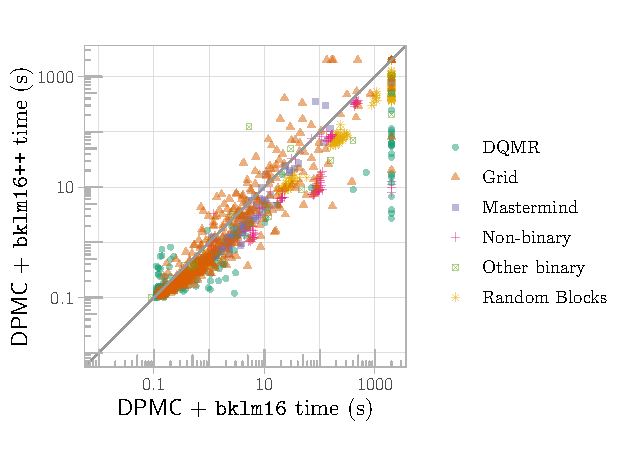
\includegraphics[width=\textwidth]{scatter2}
\end{frame}

\begin{frame}{First-Order Logic and Recursive Computations}
  \begin{example}[Counting \structure{$P\colon M \to N$} Injections]
    \begin{columns}
      \begin{column}{0.7\textwidth}
        \begin{block}{Input Formula}
          \begin{gather*}
            \forall x \in M\text{. }\exists y \in N\text{. }P(x, y) \\
            \forall x \in M\text{. }\forall y, z \in N\text{. }P(x, y) \land P(x, z) \Rightarrow y=z \\
            \forall w, x \in M\text{. }\forall y \in N\text{. }P(w, y) \land P(x, y) \Rightarrow w=x
          \end{gather*}
        \end{block}
      \end{column}
      \begin{column}{0.3\textwidth}
        \centering
        \begin{tikzpicture}[every node/.style={draw,ellipse},edge from parent/.style={draw,-latex},sibling distance=10mm,level distance=10mm]
          \node[fill=red!50] (dr) {}
          child {node {}
            child {node[fill=red!50] {}
              child {node {}
                child {node {}}
                child {node[fill=red!50] (ref) {}}
              }}};
          \draw[-latex, bend right,red] (ref) to (dr);
        \end{tikzpicture}
      \end{column}
    \end{columns}
    \begin{block}{Recursive Solution}
    \[
      f(m, n) =
      \begin{cases}
        1 & \text{if } m = 0 \text{ and } n = 0 \\
        0 & \text{if } m > 0 \text{ and } n = 0 \\
        f(m, n-1) + m \cdot f(m-1, n-1) & \text{otherwise.}
      \end{cases}
    \]
    \end{block}
  \end{example}
\end{frame}

% \begin{frame}{First-Order Knowledge Compilation}
%   \begin{block}{Workflow Before}
%     \begin{enumerate}
%       \item Compile the formula to a \alert{circuit}
%       \item Evaluate to get the answer
%     \end{enumerate}
%   \end{block}
%   \begin{block}{Workflow After}
%     \begin{enumerate}
%       \item Compile the formula to a \alert{graph}
%       \item Extract the definitions of functions
%       \item Simplify
%       \item Supplement with \alert{base cases}
%       \item Evaluate to get the answer
%     \end{enumerate}
%   \end{block}
% \end{frame}

\begin{frame}{Resulting Improvements to Counting Functions}
  Let \structure{$M$} and \structure{$N$} be two sets with cardinalities
  \structure{$|M| = m$} and \structure{$|N| = n$}.

  The new compilation rules enable \textsc{ForcLift} to efficiently count
  \structure{$M \to N$} functions such as:
  \begin{itemize}
    \item injections in \structure{$\Theta(mn)$} time
          \begin{itemize}
            \item best: \structure{$\Theta(m)$}
          \end{itemize}
    \item partial injections in \structure{$\Theta(mn)$} time
          \begin{itemize}
            \item best: \structure{$\Theta({\min\{\, m, n \,\}}^2)$}
          \end{itemize}
          \item bijections in \structure{$\Theta(m)$} time
          \begin{itemize}
            \item \alert{optimal!}
          \end{itemize}
  \end{itemize}
\end{frame}

\begin{frame}
  \vfill
  \centering
  \begin{beamercolorbox}[sep=8pt,center,shadow=true,rounded=true]{title}
    \usebeamerfont{title}Random-Instance Experiments\par%
  \end{beamercolorbox}
  \vfill
\end{frame}

\begin{frame}{A Constraint Model for (Probabilistic) Logic Programs}
  \begin{columns}
    \hspace*{-0.7cm}\begin{column}{0.75\textwidth}
      \begin{empheq}[left ={\color{color5}\empheqlbrace}]{equation}
        \begin{align*}
      \textcolor{probability}{0.2} \prob &\textcolor{predicate}{\mathtt{stress}}(\textcolor{variable}{\mathsf{P}}) \ifff \textcolor{predicate}{\mathtt{person}}(\textcolor{variable}{\mathsf{P}}). \\
      \textcolor{probability}{0.3} \prob &\textcolor{predicate}{\mathtt{influences}}(\textcolor{variable}{\mathsf{P}_1}, \textcolor{variable}{\mathsf{P}_2}) \ifff \textcolor{predicate}{\mathtt{friend}}(\textcolor{variable}{\mathsf{P}_1}, \textcolor{variable}{\mathsf{P}_2}). \\
      \textcolor{probability}{0.1} \prob &\textcolor{predicate}{\mathtt{cancer\_spont}}(\textcolor{variable}{\mathsf{P}}) \ifff \textcolor{predicate}{\mathtt{person}}(\textcolor{variable}{\mathsf{P}}). \\
      \textcolor{probability}{0.3} \prob &\textcolor{predicate}{\mathtt{cancer\_smoke}}(\textcolor{variable}{\mathsf{P}}) \ifff \textcolor{predicate}{\mathtt{person}}(\textcolor{variable}{\mathsf{P}}). \\
                                         &\textcolor{predicate}{\mathtt{smokes}}(\textcolor{variable}{\mathsf{X}}) \ifff \textcolor{predicate}{\mathtt{stress}}(\textcolor{variable}{\mathsf{X}}). \\
                                         &\textcolor{predicate}{\mathtt{smokes}}(\textcolor{variable}{\mathsf{X}}) \ifff \textcolor{predicate}{\mathtt{smokes}}(\textcolor{variable}{\mathsf{Y}}), \textcolor{predicate}{\mathtt{influences}}(\textcolor{variable}{\mathsf{Y}}, \textcolor{variable}{\mathsf{X}}). \\
                                         &\textcolor{predicate}{\mathtt{cancer}}(\textcolor{variable}{\mathsf{P}}) \ifff \textcolor{predicate}{\mathtt{cancer\_spont}}(\textcolor{variable}{\mathsf{P}}). \\
                                         &\textcolor{predicate}{\mathtt{cancer}}(\textcolor{variable}{\mathsf{P}}) \ifff \tikz \coordinate (start);\textcolor{predicate}{\mathtt{smokes}}(\textcolor{variable}{\mathsf{P}}), \textcolor{predicate}{\mathtt{cancer\_smoke}}(\textcolor{variable}{\mathsf{P}})\tikz \coordinate (end);. \\
                                         &\textcolor{predicate}{\mathtt{person}}(\textcolor{constant}{\mathit{mary}}). \\
                                         &\textcolor{predicate}{\mathtt{person}}(\textcolor{constant}{\mathit{albert}}). \\
                                         &\textcolor{predicate}{\mathtt{friend}}(\textcolor{constant}{\mathit{albert}}, \textcolor{constant}{\mathit{mary}}).
        \end{align*}
      \end{empheq}
    \end{column}
    \begin{column}{0.25\textwidth}
      \begin{itemize}
      \item[\textcolor{predicate}{\textbullet}] predicates, arities
      \item[\textcolor{variable}{\textbullet}] variables
      \item[\textcolor{constant}{\textbullet}] constants
      \item[\textcolor{probability}{\textbullet}] probabilities
      \item[\textcolor{color5}{\textbullet}] length
      \item[\textcolor{color6}{\textbullet}] complexity
      \end{itemize}
    \end{column}
  \end{columns}
  \begin{tikzpicture}[overlay]
    \draw [decorate,decoration={brace,amplitude=10pt,mirror},color=color6] (start) -- (end);
  \end{tikzpicture}
\end{frame}

\begin{frame}{\textsc{ProbLog} Inference Algorithms on Random Instances}
  \centering
  % Created by tikzDevice version 0.12.3 on 2020-05-15 17:19:15
% !TEX encoding = UTF-8 Unicode
\begin{tikzpicture}[x=1pt,y=1pt]
\definecolor{fillColor}{RGB}{255,255,255}
\path[use as bounding box,fill=fillColor,fill opacity=0.00] (0,0) rectangle (346.90,130.09);
\begin{scope}
\path[clip] (  0.00,  0.00) rectangle (346.90,130.09);
\definecolor{drawColor}{RGB}{255,255,255}
\definecolor{fillColor}{RGB}{255,255,255}

\path[draw=drawColor,line width= 0.6pt,line join=round,line cap=round,fill=fillColor] (  0.00,  0.00) rectangle (346.90,130.09);
\end{scope}
\begin{scope}
\path[clip] ( 31.71, 30.69) rectangle (146.09,108.01);
\definecolor{fillColor}{RGB}{255,255,255}

\path[fill=fillColor] ( 31.71, 30.69) rectangle (146.09,108.01);
\definecolor{drawColor}{gray}{0.92}

\path[draw=drawColor,line width= 0.3pt,line join=round] ( 31.71, 46.03) --
	(146.09, 46.03);

\path[draw=drawColor,line width= 0.3pt,line join=round] ( 31.71, 69.81) --
	(146.09, 69.81);

\path[draw=drawColor,line width= 0.3pt,line join=round] ( 31.71, 93.59) --
	(146.09, 93.59);

\path[draw=drawColor,line width= 0.3pt,line join=round] ( 49.77, 30.69) --
	( 49.77,108.01);

\path[draw=drawColor,line width= 0.3pt,line join=round] ( 75.80, 30.69) --
	( 75.80,108.01);

\path[draw=drawColor,line width= 0.3pt,line join=round] (101.84, 30.69) --
	(101.84,108.01);

\path[draw=drawColor,line width= 0.3pt,line join=round] (127.87, 30.69) --
	(127.87,108.01);

\path[draw=drawColor,line width= 0.6pt,line join=round] ( 31.71, 34.14) --
	(146.09, 34.14);

\path[draw=drawColor,line width= 0.6pt,line join=round] ( 31.71, 57.92) --
	(146.09, 57.92);

\path[draw=drawColor,line width= 0.6pt,line join=round] ( 31.71, 81.70) --
	(146.09, 81.70);

\path[draw=drawColor,line width= 0.6pt,line join=round] ( 31.71,105.48) --
	(146.09,105.48);

\path[draw=drawColor,line width= 0.6pt,line join=round] ( 36.75, 30.69) --
	( 36.75,108.01);

\path[draw=drawColor,line width= 0.6pt,line join=round] ( 62.79, 30.69) --
	( 62.79,108.01);

\path[draw=drawColor,line width= 0.6pt,line join=round] ( 88.82, 30.69) --
	( 88.82,108.01);

\path[draw=drawColor,line width= 0.6pt,line join=round] (114.85, 30.69) --
	(114.85,108.01);

\path[draw=drawColor,line width= 0.6pt,line join=round] (140.89, 30.69) --
	(140.89,108.01);
\definecolor{drawColor}{RGB}{27,158,119}

\path[draw=drawColor,line width= 0.6pt,line join=round] ( 36.91, 34.22) --
	( 37.07, 34.28) --
	( 37.38, 34.45) --
	( 37.80, 34.74) --
	( 38.00, 34.74) --
	( 39.25, 35.27) --
	( 44.64, 37.45) --
	( 44.80, 36.38) --
	( 45.11, 37.84) --
	( 47.17, 39.46) --
	( 52.37, 41.24) --
	( 52.53, 41.31) --
	( 52.84, 41.51) --
	( 60.26, 45.33) --
	( 60.58, 45.62) --
	( 67.99, 50.08) --
	( 68.15, 47.64) --
	( 68.31, 50.15) --
	( 68.46, 46.59) --
	( 69.09, 54.70) --
	( 76.04, 53.02) --
	( 83.77, 56.41) --
	( 91.50, 57.95) --
	( 99.23, 74.63) --
	( 99.55, 65.78) --
	(100.17, 64.84) --
	(130.63, 79.54) --
	(131.26, 78.48) --
	(140.89, 91.54);
\definecolor{drawColor}{RGB}{217,95,2}

\path[draw=drawColor,line width= 0.6pt,dash pattern=on 2pt off 2pt ,line join=round] ( 36.91, 34.20) --
	( 37.07, 34.26) --
	( 37.38, 34.41) --
	( 37.80, 34.70) --
	( 38.00, 34.68) --
	( 39.25, 35.23) --
	( 44.64, 37.74) --
	( 44.80, 37.05) --
	( 45.11, 37.14) --
	( 47.17, 39.19) --
	( 52.37, 42.35) --
	( 52.53, 40.98) --
	( 52.84, 41.86) --
	( 60.26, 44.75) --
	( 60.58, 45.01) --
	( 67.99, 48.70) --
	( 68.15, 46.51) --
	( 68.31, 47.05) --
	( 68.46, 47.32) --
	( 69.09, 49.64) --
	( 76.04, 52.22) --
	( 83.77, 55.11) --
	( 91.50, 58.33) --
	( 99.23, 75.16) --
	( 99.55, 59.59) --
	(100.17, 62.82) --
	(130.63, 75.24) --
	(131.26, 79.11) --
	(140.89, 88.23);
\definecolor{drawColor}{RGB}{117,112,179}

\path[draw=drawColor,line width= 0.6pt,dash pattern=on 4pt off 2pt ,line join=round] ( 36.91, 34.22) --
	( 37.07, 34.33) --
	( 37.38, 34.49) --
	( 37.80, 34.77) --
	( 38.00, 34.77) --
	( 39.25, 35.37) --
	( 44.64, 37.40) --
	( 44.80, 36.84) --
	( 45.11, 37.68) --
	( 47.17, 39.58) --
	( 52.37, 42.81) --
	( 52.53, 41.77) --
	( 52.84, 40.98) --
	( 60.26, 45.16) --
	( 60.58, 45.74) --
	( 67.99, 47.31) --
	( 68.15, 46.52) --
	( 68.31, 48.59) --
	( 68.46, 46.96) --
	( 69.09, 47.72) --
	( 76.04, 52.99) --
	( 83.77, 57.55) --
	( 91.50, 56.42) --
	( 99.23, 71.23) --
	( 99.55, 62.93) --
	(100.17, 67.49) --
	(130.63, 75.36) --
	(131.26, 79.09) --
	(140.89, 90.92);
\definecolor{drawColor}{RGB}{231,41,138}

\path[draw=drawColor,line width= 0.6pt,dash pattern=on 4pt off 4pt ,line join=round] ( 36.91, 34.22) --
	( 37.07, 34.29) --
	( 37.38, 34.48) --
	( 37.80, 34.79) --
	( 38.00, 34.74) --
	( 39.25, 35.45) --
	( 44.64, 37.64) --
	( 44.80, 37.18) --
	( 45.11, 37.98) --
	( 47.17, 40.20) --
	( 52.37, 44.88) --
	( 52.53, 42.06) --
	( 52.84, 40.35) --
	( 60.26, 45.65) --
	( 60.58, 47.25) --
	( 67.99, 51.25) --
	( 68.15, 51.16) --
	( 68.31, 51.25) --
	( 68.46, 52.79) --
	( 69.09, 51.87) --
	( 76.04, 54.08) --
	( 83.77, 57.97) --
	( 91.50, 61.03) --
	( 99.23, 76.47) --
	( 99.55, 65.20) --
	(100.17, 59.83) --
	(130.63, 84.66) --
	(131.26, 85.31) --
	(140.89, 99.29);
\definecolor{drawColor}{RGB}{102,166,30}

\path[draw=drawColor,line width= 0.6pt,dash pattern=on 1pt off 3pt ,line join=round] ( 36.91, 34.24) --
	( 37.07, 34.31) --
	( 37.38, 34.48) --
	( 37.80, 34.81) --
	( 38.00, 34.77) --
	( 39.25, 35.45) --
	( 44.64, 37.88) --
	( 44.80, 38.54) --
	( 45.11, 38.69) --
	( 47.17, 39.95) --
	( 52.37, 42.70) --
	( 52.53, 41.93) --
	( 52.84, 41.20) --
	( 60.26, 46.14) --
	( 60.58, 46.43) --
	( 67.99, 50.70) --
	( 68.15, 47.87) --
	( 68.31, 50.28) --
	( 68.46, 47.98) --
	( 69.09, 52.07) --
	( 76.04, 55.24) --
	( 83.77, 59.51) --
	( 91.50, 61.81) --
	( 99.23, 82.15) --
	( 99.55, 68.77) --
	(100.17, 67.98) --
	(130.63, 80.43) --
	(131.26, 80.51) --
	(140.89, 97.30);
\definecolor{drawColor}{RGB}{230,171,2}

\path[draw=drawColor,line width= 0.6pt,dash pattern=on 1pt off 3pt on 4pt off 3pt ,line join=round] ( 36.91, 34.20) --
	( 37.07, 34.32) --
	( 37.38, 34.47) --
	( 37.80, 34.80) --
	( 38.00, 34.78) --
	( 39.25, 35.44) --
	( 44.64, 37.83) --
	( 44.80, 36.07) --
	( 45.11, 38.73) --
	( 47.17, 40.20) --
	( 52.37, 44.23) --
	( 52.53, 43.29) --
	( 52.84, 40.97) --
	( 60.26, 46.70) --
	( 60.58, 47.28) --
	( 67.99, 50.76) --
	( 68.15, 52.81) --
	( 68.31, 51.86) --
	( 68.46, 53.84) --
	( 69.09, 51.03) --
	( 76.04, 54.08) --
	( 83.77, 59.44) --
	( 91.50, 63.01) --
	( 99.23, 79.72) --
	( 99.55, 66.18) --
	(100.17, 66.97) --
	(130.63, 83.22) --
	(131.26, 87.08) --
	(140.89, 98.99);
\definecolor{drawColor}{gray}{0.20}

\path[draw=drawColor,line width= 0.6pt,line join=round,line cap=round] ( 31.71, 30.69) rectangle (146.09,108.01);
\end{scope}
\begin{scope}
\path[clip] (151.59, 30.69) rectangle (265.96,108.01);
\definecolor{fillColor}{RGB}{255,255,255}

\path[fill=fillColor] (151.59, 30.69) rectangle (265.96,108.01);
\definecolor{drawColor}{gray}{0.92}

\path[draw=drawColor,line width= 0.3pt,line join=round] (151.59, 46.03) --
	(265.96, 46.03);

\path[draw=drawColor,line width= 0.3pt,line join=round] (151.59, 69.81) --
	(265.96, 69.81);

\path[draw=drawColor,line width= 0.3pt,line join=round] (151.59, 93.59) --
	(265.96, 93.59);

\path[draw=drawColor,line width= 0.3pt,line join=round] (169.78, 30.69) --
	(169.78,108.01);

\path[draw=drawColor,line width= 0.3pt,line join=round] (195.78, 30.69) --
	(195.78,108.01);

\path[draw=drawColor,line width= 0.3pt,line join=round] (221.77, 30.69) --
	(221.77,108.01);

\path[draw=drawColor,line width= 0.3pt,line join=round] (247.77, 30.69) --
	(247.77,108.01);

\path[draw=drawColor,line width= 0.6pt,line join=round] (151.59, 34.14) --
	(265.96, 34.14);

\path[draw=drawColor,line width= 0.6pt,line join=round] (151.59, 57.92) --
	(265.96, 57.92);

\path[draw=drawColor,line width= 0.6pt,line join=round] (151.59, 81.70) --
	(265.96, 81.70);

\path[draw=drawColor,line width= 0.6pt,line join=round] (151.59,105.48) --
	(265.96,105.48);

\path[draw=drawColor,line width= 0.6pt,line join=round] (156.79, 30.69) --
	(156.79,108.01);

\path[draw=drawColor,line width= 0.6pt,line join=round] (182.78, 30.69) --
	(182.78,108.01);

\path[draw=drawColor,line width= 0.6pt,line join=round] (208.77, 30.69) --
	(208.77,108.01);

\path[draw=drawColor,line width= 0.6pt,line join=round] (234.77, 30.69) --
	(234.77,108.01);

\path[draw=drawColor,line width= 0.6pt,line join=round] (260.76, 30.69) --
	(260.76,108.01);
\definecolor{drawColor}{RGB}{27,158,119}

\path[draw=drawColor,line width= 0.6pt,line join=round] (156.79, 87.17) --
	(160.50, 93.17) --
	(167.93, 93.97) --
	(171.64, 85.86) --
	(174.11, 95.63) --
	(186.49, 90.99) --
	(190.21, 86.16) --
	(201.35, 88.72) --
	(212.49, 93.71) --
	(216.20, 85.21) --
	(219.91, 88.26) --
	(226.10, 81.94) --
	(227.34, 84.46) --
	(231.05, 82.43) --
	(234.77, 92.42) --
	(238.48, 95.04) --
	(242.19, 93.76) --
	(253.34, 84.82) --
	(257.05, 89.64) --
	(260.76, 94.51);
\definecolor{drawColor}{RGB}{217,95,2}

\path[draw=drawColor,line width= 0.6pt,dash pattern=on 2pt off 2pt ,line join=round] (156.79, 81.98) --
	(160.50, 87.03) --
	(167.93, 90.51) --
	(171.64, 84.86) --
	(174.11, 90.95) --
	(186.49, 87.07) --
	(190.21, 82.10) --
	(201.35, 86.31) --
	(212.49, 91.58) --
	(216.20, 81.17) --
	(219.91, 86.92) --
	(226.10, 82.36) --
	(227.34, 81.20) --
	(231.05, 82.46) --
	(234.77, 88.61) --
	(238.48, 93.14) --
	(242.19, 91.31) --
	(253.34, 83.85) --
	(257.05, 86.37) --
	(260.76, 89.25);
\definecolor{drawColor}{RGB}{117,112,179}

\path[draw=drawColor,line width= 0.6pt,dash pattern=on 4pt off 2pt ,line join=round] (156.79, 88.97) --
	(160.50, 89.35) --
	(167.93, 92.54) --
	(171.64, 85.10) --
	(174.11, 93.89) --
	(186.49, 90.38) --
	(190.21, 87.37) --
	(201.35, 88.45) --
	(212.49, 94.07) --
	(216.20, 82.90) --
	(219.91, 88.35) --
	(226.10, 81.32) --
	(227.34, 84.81) --
	(231.05, 85.30) --
	(234.77, 90.02) --
	(238.48, 93.14) --
	(242.19, 94.41) --
	(253.34, 85.94) --
	(257.05, 89.62) --
	(260.76, 93.56);
\definecolor{drawColor}{RGB}{231,41,138}

\path[draw=drawColor,line width= 0.6pt,dash pattern=on 4pt off 4pt ,line join=round] (156.79, 95.74) --
	(160.50, 96.35) --
	(167.93,104.50) --
	(171.64, 94.79) --
	(174.11,102.91) --
	(186.49,101.65) --
	(190.21, 94.35) --
	(201.35, 98.68) --
	(212.49,103.55) --
	(216.20, 88.20) --
	(219.91, 97.47) --
	(226.10, 89.92) --
	(227.34, 91.22) --
	(231.05, 87.06) --
	(234.77, 98.75) --
	(238.48,102.58) --
	(242.19,102.50) --
	(253.34, 90.37) --
	(257.05, 96.15) --
	(260.76,100.82);
\definecolor{drawColor}{RGB}{102,166,30}

\path[draw=drawColor,line width= 0.6pt,dash pattern=on 1pt off 3pt ,line join=round] (156.79, 90.34) --
	(160.50,100.33) --
	(167.93, 97.34) --
	(171.64, 90.63) --
	(174.11, 99.99) --
	(186.49, 96.75) --
	(190.21, 91.32) --
	(201.35, 97.00) --
	(212.49,100.90) --
	(216.20, 88.11) --
	(219.91, 94.51) --
	(226.10, 92.66) --
	(227.34, 90.99) --
	(231.05, 92.19) --
	(234.77, 96.98) --
	(238.48, 99.26) --
	(242.19,100.29) --
	(253.34, 92.01) --
	(257.05, 93.41) --
	(260.76, 99.52);
\definecolor{drawColor}{RGB}{230,171,2}

\path[draw=drawColor,line width= 0.6pt,dash pattern=on 1pt off 3pt on 4pt off 3pt ,line join=round] (156.79, 90.96) --
	(160.50, 96.67) --
	(167.93,104.39) --
	(171.64, 90.59) --
	(174.11,102.58) --
	(186.49,100.48) --
	(190.21, 95.50) --
	(201.35, 97.48) --
	(212.49,103.31) --
	(216.20, 90.87) --
	(219.91, 97.96) --
	(226.10, 87.48) --
	(227.34, 91.85) --
	(231.05, 91.08) --
	(234.77, 98.02) --
	(238.48,100.29) --
	(242.19,102.81) --
	(253.34, 90.81) --
	(257.05, 95.58) --
	(260.76,101.07);
\definecolor{drawColor}{gray}{0.20}

\path[draw=drawColor,line width= 0.6pt,line join=round,line cap=round] (151.59, 30.69) rectangle (265.96,108.01);
\end{scope}
\begin{scope}
\path[clip] ( 31.71,108.01) rectangle (146.09,124.59);
\definecolor{drawColor}{gray}{0.20}
\definecolor{fillColor}{gray}{0.85}

\path[draw=drawColor,line width= 0.6pt,line join=round,line cap=round,fill=fillColor] ( 31.71,108.01) rectangle (146.09,124.59);
\definecolor{drawColor}{gray}{0.10}

\node[text=drawColor,anchor=base,inner sep=0pt, outer sep=0pt, scale=  0.88] at ( 88.90,113.27) {The number of facts ($\times 10^3$)};
\end{scope}
\begin{scope}
\path[clip] (151.59,108.01) rectangle (265.96,124.59);
\definecolor{drawColor}{gray}{0.20}
\definecolor{fillColor}{gray}{0.85}

\path[draw=drawColor,line width= 0.6pt,line join=round,line cap=round,fill=fillColor] (151.59,108.01) rectangle (265.96,124.59);
\definecolor{drawColor}{gray}{0.10}

\node[text=drawColor,anchor=base,inner sep=0pt, outer sep=0pt, scale=  0.88] at (208.77,113.27) {Proportion of independent pairs};
\end{scope}
\begin{scope}
\path[clip] (  0.00,  0.00) rectangle (346.90,130.09);
\definecolor{drawColor}{gray}{0.20}

\path[draw=drawColor,line width= 0.6pt,line join=round] ( 36.75, 27.94) --
	( 36.75, 30.69);

\path[draw=drawColor,line width= 0.6pt,line join=round] ( 62.79, 27.94) --
	( 62.79, 30.69);

\path[draw=drawColor,line width= 0.6pt,line join=round] ( 88.82, 27.94) --
	( 88.82, 30.69);

\path[draw=drawColor,line width= 0.6pt,line join=round] (114.85, 27.94) --
	(114.85, 30.69);

\path[draw=drawColor,line width= 0.6pt,line join=round] (140.89, 27.94) --
	(140.89, 30.69);
\end{scope}
\begin{scope}
\path[clip] (  0.00,  0.00) rectangle (346.90,130.09);
\definecolor{drawColor}{gray}{0.30}

\node[text=drawColor,anchor=base,inner sep=0pt, outer sep=0pt, scale=  0.88] at ( 36.75, 19.68) {0};

\node[text=drawColor,anchor=base,inner sep=0pt, outer sep=0pt, scale=  0.88] at ( 62.79, 19.68) {25};

\node[text=drawColor,anchor=base,inner sep=0pt, outer sep=0pt, scale=  0.88] at ( 88.82, 19.68) {50};

\node[text=drawColor,anchor=base,inner sep=0pt, outer sep=0pt, scale=  0.88] at (114.85, 19.68) {75};

\node[text=drawColor,anchor=base,inner sep=0pt, outer sep=0pt, scale=  0.88] at (140.89, 19.68) {100};
\end{scope}
\begin{scope}
\path[clip] (  0.00,  0.00) rectangle (346.90,130.09);
\definecolor{drawColor}{gray}{0.20}

\path[draw=drawColor,line width= 0.6pt,line join=round] (156.79, 27.94) --
	(156.79, 30.69);

\path[draw=drawColor,line width= 0.6pt,line join=round] (182.78, 27.94) --
	(182.78, 30.69);

\path[draw=drawColor,line width= 0.6pt,line join=round] (208.77, 27.94) --
	(208.77, 30.69);

\path[draw=drawColor,line width= 0.6pt,line join=round] (234.77, 27.94) --
	(234.77, 30.69);

\path[draw=drawColor,line width= 0.6pt,line join=round] (260.76, 27.94) --
	(260.76, 30.69);
\end{scope}
\begin{scope}
\path[clip] (  0.00,  0.00) rectangle (346.90,130.09);
\definecolor{drawColor}{gray}{0.30}

\node[text=drawColor,anchor=base,inner sep=0pt, outer sep=0pt, scale=  0.88] at (156.79, 19.68) {0};

\node[text=drawColor,anchor=base,inner sep=0pt, outer sep=0pt, scale=  0.88] at (182.78, 19.68) {0.25};

\node[text=drawColor,anchor=base,inner sep=0pt, outer sep=0pt, scale=  0.88] at (208.77, 19.68) {0.5};

\node[text=drawColor,anchor=base,inner sep=0pt, outer sep=0pt, scale=  0.88] at (234.77, 19.68) {0.75};

\node[text=drawColor,anchor=base,inner sep=0pt, outer sep=0pt, scale=  0.88] at (260.76, 19.68) {1};
\end{scope}
\begin{scope}
\path[clip] (  0.00,  0.00) rectangle (346.90,130.09);
\definecolor{drawColor}{gray}{0.30}

\node[text=drawColor,anchor=base east,inner sep=0pt, outer sep=0pt, scale=  0.88] at ( 26.76, 31.11) {0};

\node[text=drawColor,anchor=base east,inner sep=0pt, outer sep=0pt, scale=  0.88] at ( 26.76, 54.89) {10};

\node[text=drawColor,anchor=base east,inner sep=0pt, outer sep=0pt, scale=  0.88] at ( 26.76, 78.67) {20};

\node[text=drawColor,anchor=base east,inner sep=0pt, outer sep=0pt, scale=  0.88] at ( 26.76,102.45) {30};
\end{scope}
\begin{scope}
\path[clip] (  0.00,  0.00) rectangle (346.90,130.09);
\definecolor{drawColor}{gray}{0.20}

\path[draw=drawColor,line width= 0.6pt,line join=round] ( 28.96, 34.14) --
	( 31.71, 34.14);

\path[draw=drawColor,line width= 0.6pt,line join=round] ( 28.96, 57.92) --
	( 31.71, 57.92);

\path[draw=drawColor,line width= 0.6pt,line join=round] ( 28.96, 81.70) --
	( 31.71, 81.70);

\path[draw=drawColor,line width= 0.6pt,line join=round] ( 28.96,105.48) --
	( 31.71,105.48);
\end{scope}
\begin{scope}
\path[clip] (  0.00,  0.00) rectangle (346.90,130.09);
\definecolor{drawColor}{RGB}{0,0,0}

\node[text=drawColor,rotate= 90.00,anchor=base,inner sep=0pt, outer sep=0pt, scale=  1.10] at ( 13.08, 69.35) {Mean inference time (s)};
\end{scope}
\begin{scope}
\path[clip] (  0.00,  0.00) rectangle (346.90,130.09);
\definecolor{fillColor}{RGB}{255,255,255}

\path[fill=fillColor] (276.96, 12.88) rectangle (341.40,125.82);
\end{scope}
\begin{scope}
\path[clip] (  0.00,  0.00) rectangle (346.90,130.09);
\definecolor{drawColor}{RGB}{0,0,0}

\node[text=drawColor,anchor=base west,inner sep=0pt, outer sep=0pt, scale=  1.10] at (282.46,111.67) {Algorithm};
\end{scope}
\begin{scope}
\path[clip] (  0.00,  0.00) rectangle (346.90,130.09);
\definecolor{fillColor}{RGB}{255,255,255}

\path[fill=fillColor] (282.46, 90.65) rectangle (296.92,105.10);
\end{scope}
\begin{scope}
\path[clip] (  0.00,  0.00) rectangle (346.90,130.09);
\definecolor{drawColor}{RGB}{27,158,119}

\path[draw=drawColor,line width= 0.6pt,line join=round] (283.91, 97.88) -- (295.47, 97.88);
\end{scope}
\begin{scope}
\path[clip] (  0.00,  0.00) rectangle (346.90,130.09);
\definecolor{fillColor}{RGB}{255,255,255}

\path[fill=fillColor] (282.46, 76.20) rectangle (296.92, 90.65);
\end{scope}
\begin{scope}
\path[clip] (  0.00,  0.00) rectangle (346.90,130.09);
\definecolor{drawColor}{RGB}{217,95,2}

\path[draw=drawColor,line width= 0.6pt,dash pattern=on 2pt off 2pt ,line join=round] (283.91, 83.42) -- (295.47, 83.42);
\end{scope}
\begin{scope}
\path[clip] (  0.00,  0.00) rectangle (346.90,130.09);
\definecolor{fillColor}{RGB}{255,255,255}

\path[fill=fillColor] (282.46, 61.74) rectangle (296.92, 76.20);
\end{scope}
\begin{scope}
\path[clip] (  0.00,  0.00) rectangle (346.90,130.09);
\definecolor{drawColor}{RGB}{117,112,179}

\path[draw=drawColor,line width= 0.6pt,dash pattern=on 4pt off 2pt ,line join=round] (283.91, 68.97) -- (295.47, 68.97);
\end{scope}
\begin{scope}
\path[clip] (  0.00,  0.00) rectangle (346.90,130.09);
\definecolor{fillColor}{RGB}{255,255,255}

\path[fill=fillColor] (282.46, 47.29) rectangle (296.92, 61.74);
\end{scope}
\begin{scope}
\path[clip] (  0.00,  0.00) rectangle (346.90,130.09);
\definecolor{drawColor}{RGB}{231,41,138}

\path[draw=drawColor,line width= 0.6pt,dash pattern=on 4pt off 4pt ,line join=round] (283.91, 54.52) -- (295.47, 54.52);
\end{scope}
\begin{scope}
\path[clip] (  0.00,  0.00) rectangle (346.90,130.09);
\definecolor{fillColor}{RGB}{255,255,255}

\path[fill=fillColor] (282.46, 32.83) rectangle (296.92, 47.29);
\end{scope}
\begin{scope}
\path[clip] (  0.00,  0.00) rectangle (346.90,130.09);
\definecolor{drawColor}{RGB}{102,166,30}

\path[draw=drawColor,line width= 0.6pt,dash pattern=on 1pt off 3pt ,line join=round] (283.91, 40.06) -- (295.47, 40.06);
\end{scope}
\begin{scope}
\path[clip] (  0.00,  0.00) rectangle (346.90,130.09);
\definecolor{fillColor}{RGB}{255,255,255}

\path[fill=fillColor] (282.46, 18.38) rectangle (296.92, 32.83);
\end{scope}
\begin{scope}
\path[clip] (  0.00,  0.00) rectangle (346.90,130.09);
\definecolor{drawColor}{RGB}{230,171,2}

\path[draw=drawColor,line width= 0.6pt,dash pattern=on 1pt off 3pt on 4pt off 3pt ,line join=round] (283.91, 25.61) -- (295.47, 25.61);
\end{scope}
\begin{scope}
\path[clip] (  0.00,  0.00) rectangle (346.90,130.09);
\definecolor{drawColor}{RGB}{0,0,0}

\node[text=drawColor,anchor=base west,inner sep=0pt, outer sep=0pt, scale=  0.88] at (302.42, 94.85) {BDD};
\end{scope}
\begin{scope}
\path[clip] (  0.00,  0.00) rectangle (346.90,130.09);
\definecolor{drawColor}{RGB}{0,0,0}

\node[text=drawColor,anchor=base west,inner sep=0pt, outer sep=0pt, scale=  0.88] at (302.42, 80.39) {d-DNNF};
\end{scope}
\begin{scope}
\path[clip] (  0.00,  0.00) rectangle (346.90,130.09);
\definecolor{drawColor}{RGB}{0,0,0}

\node[text=drawColor,anchor=base west,inner sep=0pt, outer sep=0pt, scale=  0.88] at (302.42, 65.94) {K-Best};
\end{scope}
\begin{scope}
\path[clip] (  0.00,  0.00) rectangle (346.90,130.09);
\definecolor{drawColor}{RGB}{0,0,0}

\node[text=drawColor,anchor=base west,inner sep=0pt, outer sep=0pt, scale=  0.88] at (302.42, 51.49) {NNF};
\end{scope}
\begin{scope}
\path[clip] (  0.00,  0.00) rectangle (346.90,130.09);
\definecolor{drawColor}{RGB}{0,0,0}

\node[text=drawColor,anchor=base west,inner sep=0pt, outer sep=0pt, scale=  0.88] at (302.42, 37.03) {SDD};
\end{scope}
\begin{scope}
\path[clip] (  0.00,  0.00) rectangle (346.90,130.09);
\definecolor{drawColor}{RGB}{0,0,0}

\node[text=drawColor,anchor=base west,inner sep=0pt, outer sep=0pt, scale=  0.88] at (302.42, 22.58) {SDDX};
\end{scope}
\end{tikzpicture}

\end{frame}

\begin{frame}{Random WMC Instances}
  \begin{block}{Key Idea}
    Parameter \structure{$\rho \in [0, 1]$} biases the probability distribution
    towards adding variables that would introduce fewer new edges in the primal
    graph.
  \end{block}
  \begin{example}
    \begin{columns}
      \begin{column}{0.65\linewidth}
        Partially-constructed formula:
        \[
          (\neg x_{5} \lor x_{2} \lor x_{1}) \land (x_{5} \lor \alert{\mathord{?}} \lor \mathord{?}).
        \]
      \end{column}
      \begin{column}{0.25\linewidth}
        Its primal graph:

        \begin{tikzpicture}
          \node (a) at (0.5, 1) {$x_{1}$};
          \node (b) at (0, 0) {$x_{2}$};
          \node (c) at (1, 0) {\spot{$x_{5}$}};
          \node (d) at (2, 1) {$x_{3}$};
          \node (e) at (2, 0) {$x_{4}$};
          \draw (a) -- (b);
          \draw[blue,thick] (b) -- (c);
          \draw[blue,thick] (c) -- (a);
          \draw (current bounding box.north east) rectangle (current bounding box.south west);
        \end{tikzpicture}
      \end{column}
    \end{columns}

    Base probability of each variable being chosen:
    \[
      \frac{1 - \rho}{4}.
    \]

    Both \structure{$x_{1}$} and \structure{$x_{2}$} get a bonus probability of
    \structure{$\rho/2$} for each being the endpoint of \alert{one} out of
    the \alert{two} neighbourhood edges.
  \end{example}
\end{frame}

 \begin{frame}{How WMC Algorithms Scale w.r.t. Primal Treewidth}
  We fit the model \structure{$\ln t \sim \alpha w + \beta$}, i.e.,
  \structure{$t \sim e^{\beta}{(e^{\alpha})}^{w}$}, where \structure{$t$} is
  \alert{runtime}, and \structure{$w$} is \alert{primal treewidth}.

  \centering
  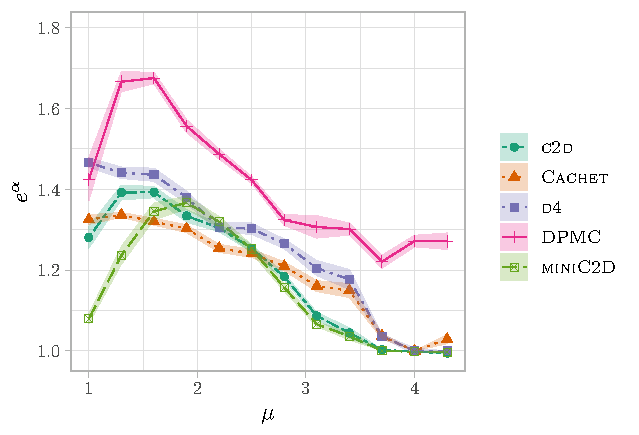
\includegraphics{linearbase.pdf}
\end{frame}

% Mention the applicability of WMC and the two main strands of my contributions
\begin{frame}{Summary}
  \begin{block}{What Have We Learned?}
    \begin{itemize}
      \item Pseudo-Boolean functions as an alternative to literal weights
      \item Cycles in graphs that encode recursive calls
      \item WMC is not always the bottleneck in probabilistic inference
      \item WMC algorithms based on algebraic decision diagrams are fundamentally different:
      \begin{itemize}
        \item they can supports non-literal weights
        \item their running time depends on the numerical values of weights
        \item they peak at higher density
        \item they scale worse w.r.t.\ primal treewidth
      \end{itemize}
    \end{itemize}
  \end{block}
  \begin{block}{Future Directions}
    \begin{itemize}
      \item PBP\@: new encodings, kernelization, pseudo-Boolean solvers
      \item WFOMC\@: full automation and new applications (e.g., in AI)
    \end{itemize}
  \end{block}
\end{frame}

% IMPORTANCE, ORIGINALITY, CORRECTNESS

% Originality:
% 1. Representations for WMC problems that go beyond the "CNF + literal weights" tradition (e.g., PBP)
% 2. Circuits with cycles + the 'recursive-algebraic' POV of WFOMC
% 3. Experimental studies of WMC algorithms on random instances with varying:
% a) application-specific parameters (e.g., predicate arities)
% b) parameters that determine the hardness of the problem (e.g., density and primal treewidth)

% Importance (why these things are important to study):
% What is the benefit for academic understanding, the general public, a specific avenue? Why this question in particular?
% 1. A simpler representation of a problem often leads to a faster solution. In my work, this is because ADDs are capable of representing more than just clauses.
% 2. Interpreting a circuit/graph as a collection of algebraically-defined functions highlights the kinds of computations that are not yet supported by WFOMC algorithms
% 3. Important observation: WMC is usually not the bottleneck of ProbLog inference
% 4. Important observation: ADD-based WMC algorithms are fundamentally different in that:
% a) their running time depends on the numerical values of weights
% b) they scale worse w.r.t. primal treewidth
% c) they peak at higher density

\end{document}
